\documentclass[11pt,oneside]{book}
\usepackage{fontspec}
\usepackage{xeCJK}
\setmainfont{Latin Modern Roman}
\setCJKmainfont[ItalicFont={Noto Serif CJK SC},BoldItalicFont={Noto Serif CJK SC Bold}]{Noto Serif CJK SC}
\setCJKsansfont{Noto Sans CJK SC}
\setCJKmonofont{Noto Sans Mono CJK SC}
\newfontfamily\proseunicodefont{DejaVu Serif}
\usepackage[margin=1in]{geometry}
\usepackage{microtype}
\usepackage{amsmath,amssymb,amsthm,mathtools,bm}
\usepackage{graphicx}
\usepackage{xcolor}
\usepackage{booktabs}
\usepackage{array}
\usepackage{longtable}
\usepackage{enumitem}
\usepackage{float}
\usepackage{caption}
\usepackage{hyperref}
\usepackage{fancyhdr}
\usepackage{tikz}
\usetikzlibrary{arrows.meta,positioning,calc,decorations.pathmorphing}

\hypersetup{
  colorlinks=true,
  linkcolor=blue!50!black,
  urlcolor=blue!50!black,
  citecolor=blue!50!black
}

\setlength{\parskip}{0.5em}
\setlength{\parindent}{0pt}
\setlist[itemize]{topsep=0.25em,itemsep=0.2em}
\setlist[enumerate]{topsep=0.25em,itemsep=0.2em}
\setlength{\headheight}{40pt}
\numberwithin{equation}{chapter}

\newtheorem{theorem}{定理}[chapter]
\newtheorem{proposition}[theorem]{命题}
\newtheorem{lemma}[theorem]{引理}
\newtheorem{corollary}[theorem]{推论}
\theoremstyle{definition}
\newtheorem{definition}[theorem]{定义}
\newtheorem{example}[theorem]{例}
\theoremstyle{remark}
\newtheorem{remark}[theorem]{注}

\providecommand{\ket}[1]{\left\lvert#1\right\rangle}
\providecommand{\bra}[1]{\left\langle#1\right\rvert}
\providecommand{\braket}[2]{\left\langle#1\,\middle|\,#2\right\rangle}
\providecommand{\expect}[1]{\left\langle#1\right\rangle}
\newcommand{\lectureoverview}[1]{\paragraph{概述。} #1}
\newenvironment{classroomqa}{%
  \par\medskip
  \begin{quote}\small
}{%
  \end{quote}
  \medskip
}
\newcommand{\audiencequestion}[1]{\noindent\textbf{听众提问。} #1\par\smallskip}
\newcommand{\classquestion}[1]{\noindent\textbf{课堂提问。} #1\par\smallskip}
\newcommand{\lecturerresponse}[1]{\noindent\textbf{回答。} #1\par}
\newcommand{\lecturetimestamp}[1]{\footnote{讲课时间： #1.}}
\newcommand{\lectureframe}[1]{\par\smallskip{\centering\footnotesize\itshape 讲课画面： #1.\par}}

\makeatletter
\newcommand{\course@headerfont}{\normalfont\small\itshape}
\newcommand{\course@pagefont}{\normalfont\small}
\newcommand{\course@headerraise}{14pt}
\newlength{\course@headerboxheight}
\setlength{\course@headerboxheight}{\dimexpr\headheight-\course@headerraise-9pt\relax}
\newcommand{\course@leftheadbox}[1]{%
  \raisebox{\course@headerraise}{%
    \parbox[t][\course@headerboxheight][t]{0.82\textwidth}{%
      \raggedright\course@headerfont\strut\MakeUppercase{#1}\strut%
    }%
  }%
}
\newcommand{\course@rightheadbox}[1]{%
  \raisebox{\course@headerraise}{%
    \parbox[t][\course@headerboxheight][t]{0.82\textwidth}{%
      \raggedleft\course@headerfont\strut\MakeUppercase{#1}\strut%
    }%
  }%
}
\renewcommand{\chaptermark}[1]{\markboth{\MakeUppercase{\chaptername\ \thechapter.\ #1}}{}}
\renewcommand{\sectionmark}[1]{\markright{\MakeUppercase{\thesection\hspace{0.4em}#1}}}
\fancyhf{}
\fancyhead[L]{\course@leftheadbox{\leftmark}}
\fancyhead[R]{\course@pagefont\thepage}
\renewcommand{\headrulewidth}{0.5pt}
\pagestyle{fancy}
\fancypagestyle{plain}{%
  \fancyhf{}
  \fancyhead[L]{\course@leftheadbox{\leftmark}}
  \fancyhead[R]{\course@pagefont\thepage}
  \renewcommand{\headrulewidth}{0.5pt}
}
\makeatother

\renewcommand{\contentsname}{目录}
\renewcommand{\chaptername}{章}
\renewcommand{\figurename}{图}
\renewcommand{\tablename}{表}
\renewcommand{\proofname}{证明}
\renewcommand{\bibname}{参考文献}
\emergencystretch=2em
\pdfstringdefDisableCommands{\def\proseunicodefont{}}

\graphicspath{{../../../generated_course_notes/core/statistical_mechanics/2013_spring_theoretical_minimum/figures/}{../../../generated_course_notes/core/statistical_mechanics/2013_spring_theoretical_minimum/assets/}}
\hypersetup{
  pdftitle={Statistical Mechanics: The Theoretical Minimum},
  pdfauthor={Leonard Susskind; companion notes edited by LazyingArt LLC with Video2Book},
  pdfsubject={Core track, 2013 Spring},
  pdfkeywords={Leonard Susskind, statistical mechanics, thermodynamics, Ising model, critical phenomena}
}
\begin{document}
\frontmatter
\hypersetup{pageanchor=false}
\begin{titlepage}
\thispagestyle{empty}
\begin{tikzpicture}[remember picture,overlay]
  \node[anchor=south west,inner sep=0] at (current page.south west) {%
    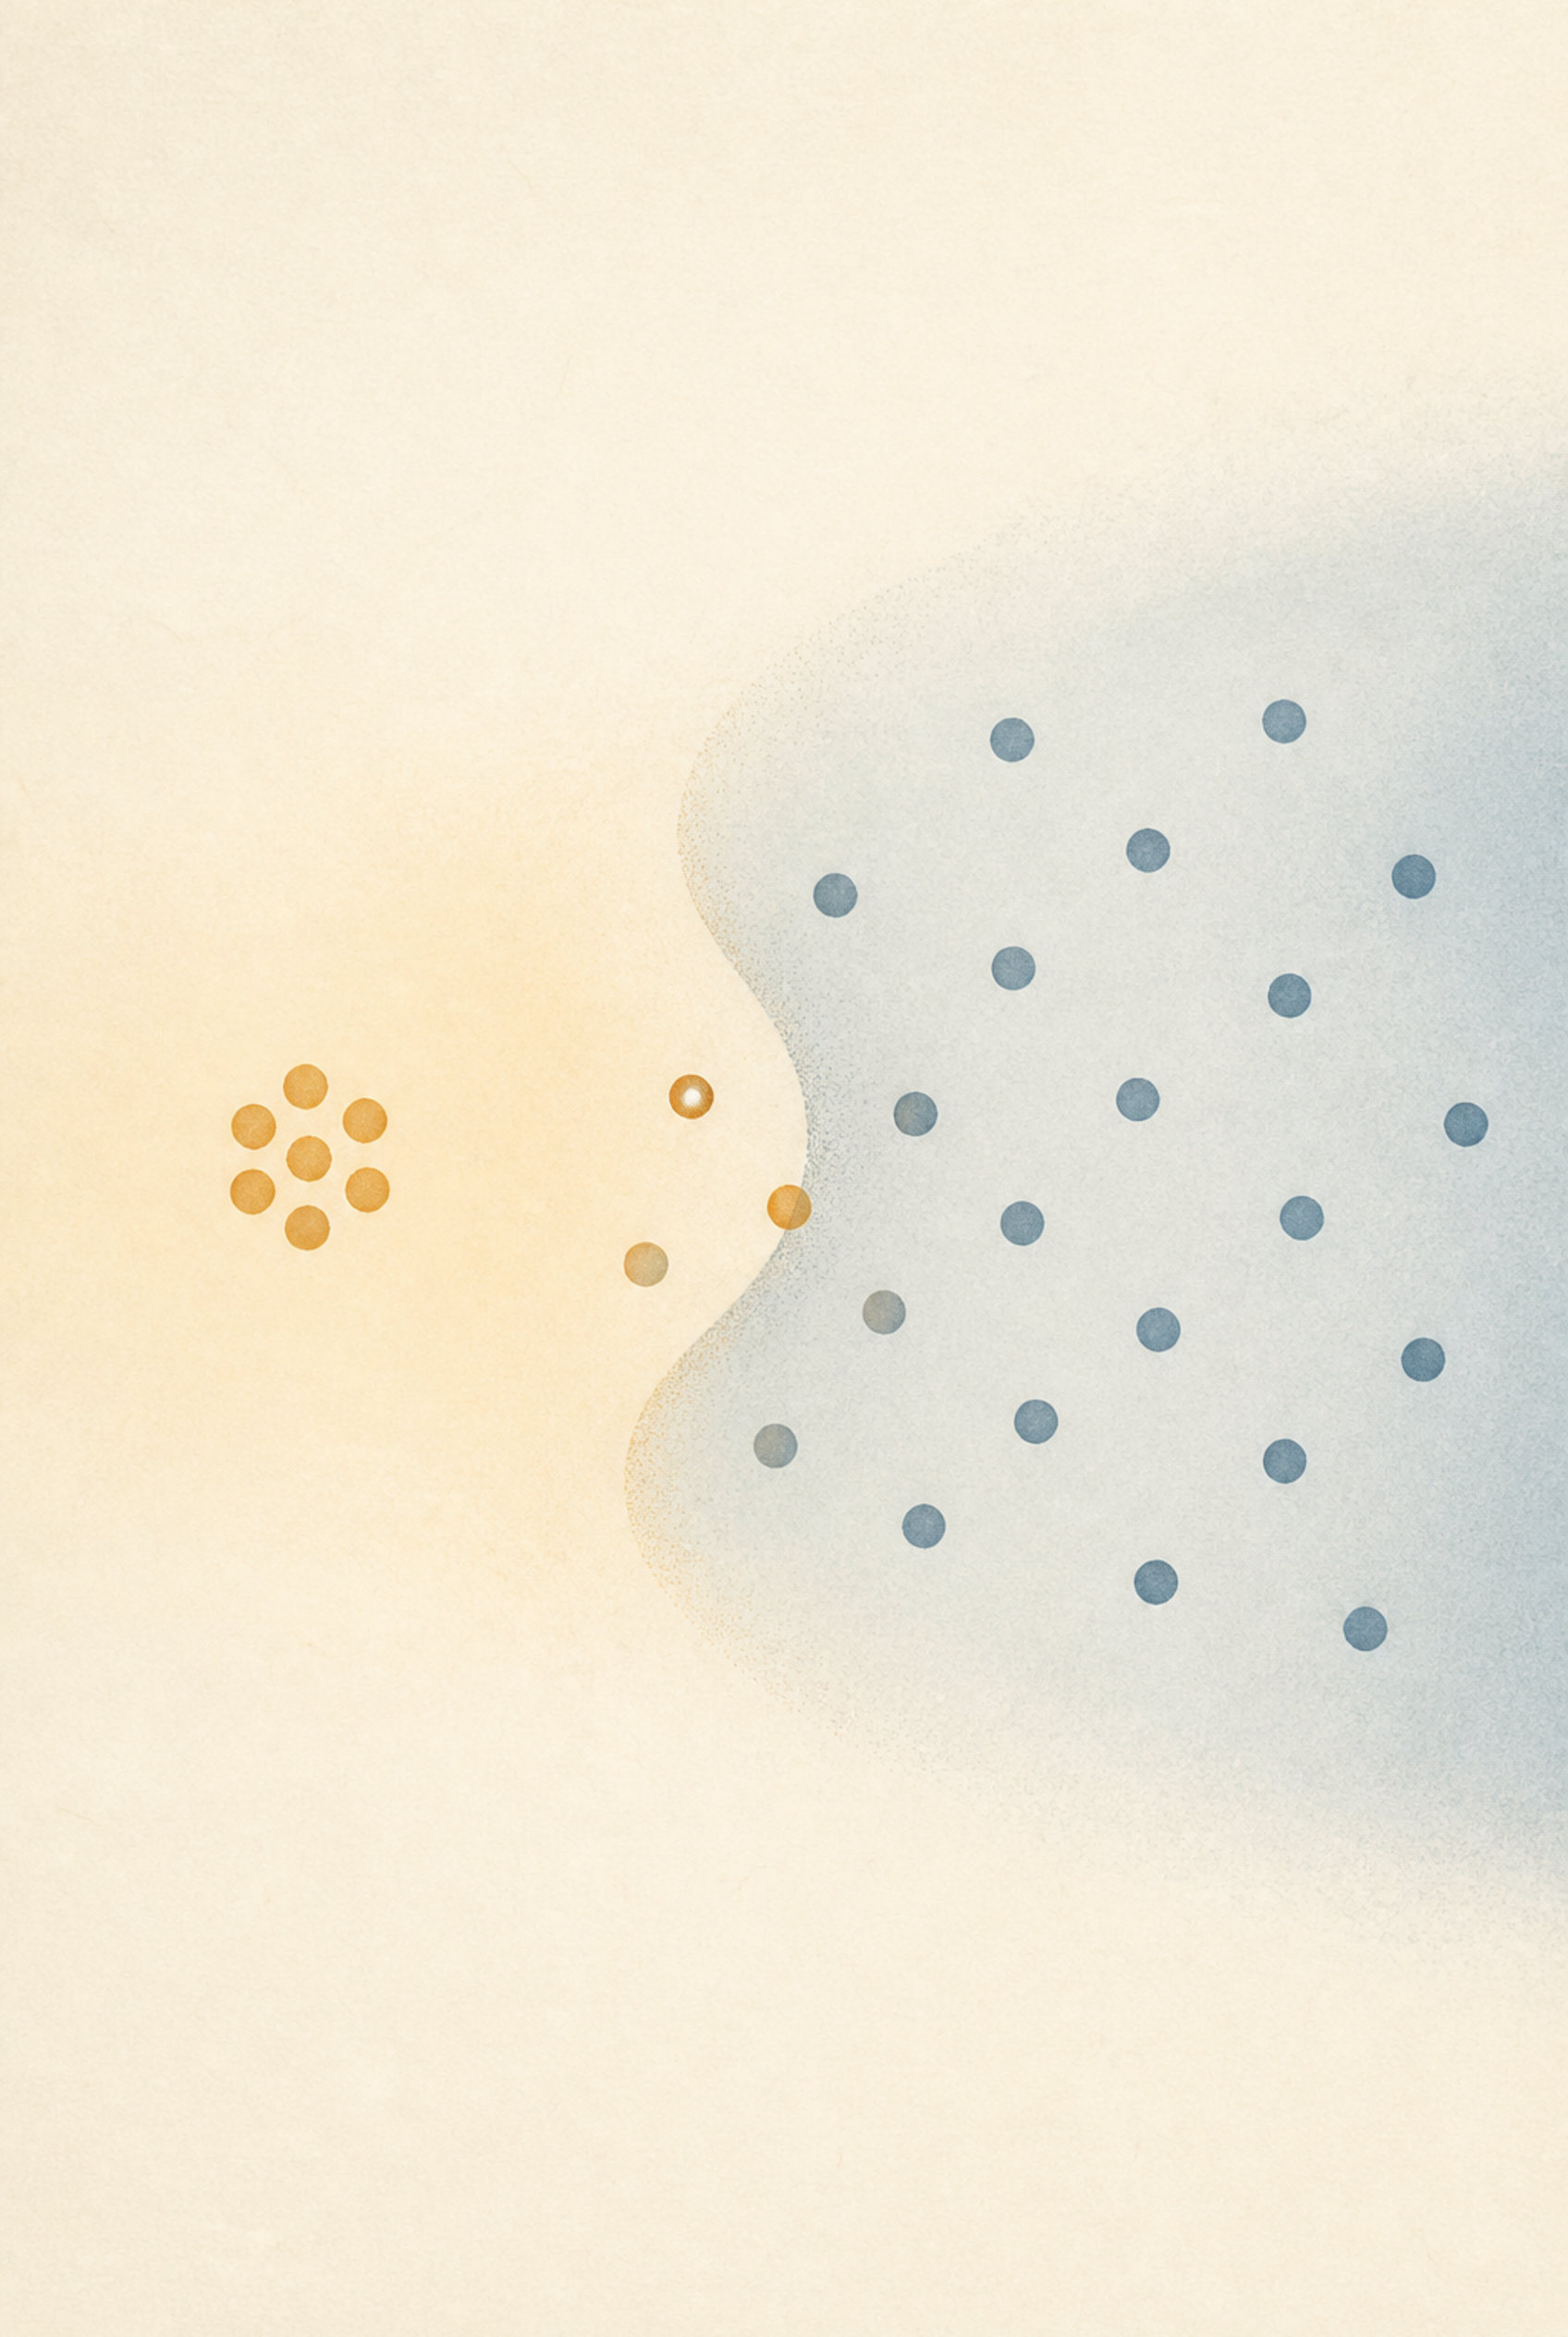
\includegraphics[width=\paperwidth,height=\paperheight,keepaspectratio=false]{../../../generated_course_notes/core/statistical_mechanics/2013_spring_theoretical_minimum/assets/cover-art.png}%
  };
  \node[
    anchor=north west,
    align=left,
    text width=0.78\paperwidth,
    fill=white,
    fill opacity=0.9,
    rounded corners=8pt,
    inner xsep=10pt,
    inner ysep=8pt
  ] at ([xshift=0.08\paperwidth,yshift=-0.06\paperheight]current page.north west) {%
    {\fontsize{30}{33}\selectfont\bfseries\color{black!88} 统计力学\\[0.85em]}
    {\large\color{black!72} 中文版 / 2013 spring theoretical minimum}
  };
  \node[
    anchor=south west,
    align=left,
    text width=0.68\paperwidth,
    fill=white,
    fill opacity=0.82,
    text opacity=1,
    rounded corners=6pt,
    inner sep=12pt
  ] at ([xshift=0.08\paperwidth,yshift=0.08\paperheight]current page.south west) {%
    {\normalsize\color{black!78} 原讲授：Leonard Susskind\\[0.35em]}
    {\small\color{black!72} 讲义辅助版本：\href{https://lazying.art}{LazyingArt LLC} / \href{https://github.com/lachlanchen/Video2Book}{Video2Book}.}
  };
\end{tikzpicture}
\mbox{}
\end{titlepage}
\hypersetup{pageanchor=true}

\chapter*{关于本讲义}
本独立编辑的配套讲义依据 Leonard Susskind 的 2013 年统计力学讲座整理而成。它们保留了讲座的讲解顺序、实质性的课堂交流、数学推导以及部分黑板记录。它们并非 Susskind 教授的原稿，也未经其审阅或认可。

本版本由 \href{https://lazying.art}{LazyingArt LLC} 使用开源 \href{https://github.com/lachlanchen/Video2Book}{Video2Book} 工作流程制作。完整的机器转录稿和字幕文件另行保存在代码库中，其中可能包含识别错误。
\clearpage
\tableofcontents
\mainmatter
\chapter{概率、信息与熵}

\lectureoverview{统计力学始于微观定律与不完全知识相遇之处。我们首先使概率变得精确，然后追问确定性运动本身如何赋予概率、守恒定律如何划分状态空间，以及为什么保信息的动力学自然地导向熵。第一定律和第零定律只有在这一结构就位之后才进入。}

\section{为什么需要统计力学？}

统计力学有时被描述为旧物理学。这种描述没有抓住要点。它既是前现代的，又是现代的，而且很可能在任何接替我们所知理论的后现代物理学中仍然有用。具体的模型来来去去；热力学第二定律却一再作为路标而存留下来。每当一种对自然的描述似乎凭空制造出秩序、从根本上抹除信息，或使一个封闭系统退化到不自然的简单状态时，第二定律就警告我们：有某种东西被遗漏了。

这门学科或许不如新发现的粒子那样引人注目，但它至少同样深刻，而且远为普遍。气体、液体、固体、辐射、黑洞、信息和量子场都需要统计推理。事实上，用来发现粒子的实验装置若没有它就无法被理解。这就是为什么一代又一代强有力的物理学家精通统计力学，即使他们的主要工作在其他领域：这门学科很有用，但它也异常优美。

要看清为什么需要它，先从力学所提供的理想情形开始。一个封闭系统要么是我们所考虑的整个宇宙，要么是一个被隔离得足够好、以致其环境不影响它的子系统。如果我们知道它的初始条件和它的演化定律，那么经典力学就提供完整的预测。量子力学修改了可被预测的内容，但它同样有一个精确定义的状态，以及一条预测该理论所允许的最大信息的定律。

原则上可预测与有用的理解之间存在严重的差别。一份列出这个房间里每个分子的位置和速度的清单会长得不可思议，几乎立刻就会改变，而且几乎回答不了我们真正关心的任何问题。因此，精确的微观定律可以同时是完全可预测的，又在实践上毫无用处。

统计力学就是应用于这种物理情形的概率论。当初始条件不被完全精确地知道时，当定律只被近似地知道时，当系统是开放的时，或者仅仅当微观变量的数目大到无法追踪时，它就成为必要的。这一切都不意味着预测薄弱。大数往往使统计预测变得异常锐利。

考虑一个孤立的气体盒子。我们无法预测每个分子的轨迹，然而少数宏观数据使我们能够高精度地预测压强、能量以及许多其他体量。仍然不确定的是涨落。在某个不可预测的时刻，一个小区域可能包含比平均更多的分子，而另一个区域包含更少。这样的事件位于概率分布的尾部：不太可能，但并非被禁止。我们可以计算这类涨落应当以多高的频率发生，而不必预测某一次具体发生的时刻。

抛硬币显示出同样的区别。在十亿次公平抛掷中，正面和反面的数目将接近相等。如果我们抛得足够频繁，一长串正面最终会出现，但概率论预测的是它的频率，而不是事先指定它的时刻。统计力学是为那些其元素太小、太多，或两者兼而有之的系统而设计的。

本课程将展开这些定律以及它们对物质的应用。这门学科值得反复学习：人们学会它，忘掉其中一部分，然后再一次学会它，并对哪些观念是根本的有了更深的感觉。我们从那个支配随后一切的观念开始。

\section{作为原始语言的概率}

概率为什么有效，并不是概率演算本身所能解释的。一个概率性预测可能在某一次试验中失败；这正是某个结果可能但不太可能的含义。该理论告诉我们例外是如何分布的。它并不消除例外。因此我们把概率当作一个原始概念，并陈述它所服从的规则。

\subsection{状态与归一化}

设\(i\)标记一个可能的结果或系统的一个可能状态。对于一枚硬币，\(i\)可以表示正面或反面。对于一颗骰子，它可以从\(1\)取到\(6\)。对于两颗骰子，一对指标记录两个面。我们从有限离散状态空间开始，
\begin{equation}
 i=1,\ldots,N,
\end{equation}
之后再过渡到无穷多个以及连续多个状态。

无知并不意味着系统没有状态。它意味着我们不知道系统处于哪个状态，因此我们为每种可能性赋予一个概率\(p_i\)。基本规则是
\begin{align}
 p_i &\geq 0, \label{eq:sm1-prob-positive}\\
 \sum_{i=1}^{N}p_i &=1. \label{eq:sm1-prob-normalization}
\end{align}
这些备选情形互斥且穷尽：其中恰好有一个发生。负概率在这里没有地位，而总和为一，因为某个允许的结果必定会发生。

\subsection{频率与大数定律}

概率通过重复试验与实验相联系。假设同一个实验进行了\(N_{\mathrm{trials}}\)次，并令\(N(i)\)为产生结果\(i\)的试验次数。那么频率解释为
\begin{equation}
 p_i=
 \lim_{N_{\mathrm{trials}}\to\infty}
 \frac{N(i)}{N_{\mathrm{trials}}}.
 \label{eq:sm1-frequency}
\end{equation}
这是一个通过理想极限表述的物理假设。没有实验室会进行无穷多次实验。其主张是，足够多的试验会使该比值稳定在足够接近\(p_i\)处，以满足预期的预测。有限样本会在极限值附近涨落。

\subsection{平均值}

现在为每个状态赋予一个数\(f(i)\)。它可以是能量、动量，或我们希望测量的任何其他量。其期望值为
\begin{equation}
 \langle f\rangle=\sum_i f(i)p_i.
 \label{eq:sm1-expectation}
\end{equation}
即使在量子力学之外，括号记号也很方便。用频率的语言，同一个平均值为
\begin{equation}
 \langle f\rangle
 =
 \lim_{N_{\mathrm{trials}}\to\infty}
 \frac{1}{N_{\mathrm{trials}}}
 \sum_i f(i)N(i).
 \label{eq:sm1-frequency-average}
\end{equation}

对于一枚硬币，定义
\begin{equation}
 f(\mathrm{H})=+1,
 \qquad
 f(\mathrm{T})=-1.
\end{equation}
如果正面和反面各有概率\(1/2\)，那么
\begin{equation}
 \langle f\rangle
 =(+1)\frac12+(-1)\frac12=0.
\end{equation}
平均值不必是一个可能的结果。硬币从不会落在零上；零概括了其两个可能取值的分布。

这段简短的插曲确定了本学科通篇使用的词汇：状态、概率、频率和期望值。

\section{赋予概率的三种方式}

\subsection{对称性}

为什么我们通常给硬币的两个面赋予相等的概率？第一个答案是对称性。将一枚近乎理想的硬币翻转会交换正面和反面，而不改变实验。于是没有物理理由偏向任一结果。真实的标记或瑕疵会引入微小的偏置，但对称模型刻画了预期的实验：
\begin{equation}
 p(\mathrm{H})=p(\mathrm{T})=\frac12.
\end{equation}

同样的论证给对称骰子的每个面赋予概率\(1/6\)。更一般地，由对称性相联系的构型被赋予相等的概率，除非某些额外信息破坏了该对称性。

\subsection{实验}

一颗形状不规则的骰子没有交换全部六个面的对称性。在这种情况下，仅靠对称性给不出答案。人们可能拥有一个更深入的力学模型来预测偏置，但若没有这样的模型，诚实的做法就是实验：多次投掷骰子，记录频率，等待它们稳定下来，并在后续预测中使用所得的概率表。

对称性和实验并不是相互竞争的定义。它们是关于一个概率分布的两种信息来源。统计力学将大量依赖对称性，但动力学提供了第三条途径。

\subsection{来自确定性运动的概率}

想象一个不规则物体，具有六种有颜色的构型。它按照确定的更新法则在固定的离散时间间隔改变状态：
\begin{equation}
 R\longrightarrow B\longrightarrow Y\longrightarrow G
 \longrightarrow O\longrightarrow P\longrightarrow R.
 \label{eq:sm1-six-cycle}
\end{equation}
该物体本身不必具有任何几何对称性。该法则只说明给定构型之后是哪个构型。

\begin{figure}[htbp]
\centering
\includegraphics[width=0.92\textwidth]{lecture_01_figure_02.png}
\caption{期望值公式留在左侧黑板上，而六个确定性颜色更新列在右侧。}
\lectureframe{00:26:28}
\end{figure}

当画成一个有向循环时，黑板上的列表更加清晰：
\begin{figure}[htbp]
\centering
\begin{tikzpicture}[
  >=Latex,
  state/.style={draw,circle,minimum size=8mm,inner sep=1pt}
]
\node[state] (R) at (90:2.2) {$R$};
\node[state] (B) at (30:2.2) {$B$};
\node[state] (Y) at (-30:2.2) {$Y$};
\node[state] (G) at (-90:2.2) {$G$};
\node[state] (O) at (-150:2.2) {$O$};
\node[state] (P) at (150:2.2) {$P$};
\draw[->] (R) -- (B);
\draw[->] (B) -- (Y);
\draw[->] (Y) -- (G);
\draw[->] (G) -- (O);
\draw[->] (O) -- (P);
\draw[->] (P) -- (R);
\end{tikzpicture}
\caption{一个单一的六状态轨道。每个周期内每个状态都被访问一次。}
\label{fig:sm1-six-cycle}
\end{figure}

假设我们不知道初始状态，并在一个未知时刻进行快照。由于每一步持续的时间相等，系统在每个颜色中度过一个周期的六分之一：
\begin{equation}
 p(R)=p(B)=p(Y)=p(G)=p(O)=p(P)=\frac16.
 \label{eq:sm1-uniform-cycle}
\end{equation}
这一相等并非来自物体的形状。它来自在各状态中度过的相等时间。

我们可以重新排列箭头，得到一种不同的微观法则，同时仍然形成一个六状态循环。具体顺序改变了，但快照概率仍为\(1/6\)，因为每个状态在每个周期中仍然出现一次。因此这一预测既不需要起点，也不需要具体顺序。它只需要轨道结构以及每次更新所对应的相等时间。

\begin{classroomqa}
\classquestion{如果物体并不对称，那么在什么意义上给每种颜色赋予概率\(1/6\)才是合理的？}
\lecturerresponse{这种赋值是动力学性的，而非几何性的。在一个六步轨道上未知相位处拍摄的快照，采样的是六个等长的时间槽。相关的等价性在于轨道上的位置之间，而不在于物体的各个面之间。如果停留时间不相等，概率也会不相等。
\lecturetimestamp{00:27:11--00:29:49}}
\end{classroomqa}

\section{不连通的循环与守恒量}

确定性定律不必把所有状态都放在同一条轨道上。考虑两个不连通的循环，
\begin{equation}
 R\longrightarrow B\longrightarrow G\longrightarrow R,
 \qquad
 P\longrightarrow Y\longrightarrow O\longrightarrow P.
 \label{eq:sm1-two-cycles}
\end{equation}
如果我们知道系统位于第一个循环上，那么
\begin{equation}
 \begin{aligned}
 p(R)=p(B)=p(G)&=\frac13,\\
 p(P)=p(Y)=p(O)&=0.
 \end{aligned}
\end{equation}
知道它位于第二个循环上则把这些赋值颠倒过来。

更一般的情形需要先验权重。把两个循环分别标记为\(+1\)和\(-1\)，并设它们的概率为\(p_+\)和\(p_-\)，且满足
\begin{equation}
 p_++p_-=1.
\end{equation}
于是
\begin{align}
 p(R)=p(B)=p(G)&=\frac{p_+}{3},\\
 p(P)=p(Y)=p(O)&=\frac{p_-}{3}.
 \label{eq:sm1-sector-weights}
\end{align}
因子\(1/3\)来自循环内部的运动。而数\(p_+\)和\(p_-\)则不然。它们必须来自额外的知识，也许是另一个实验，或是另一个选定初始扇区的系统。

标记\(+1\)和\(-1\)定义了一个守恒量：一旦系统从某个循环出发，更新定律绝不会把它带到另一个循环。人们可以把这个量称为能量，或者给它一个占位名称，比如\emph{zilch}。它的名称是次要的。守恒意味着状态空间被划分为动力学无法跨越的区域。

这些循环不必包含相同数目的状态。一个四态轨道和一个二态轨道仍然定义两个守恒扇区。等时采样于是在第一个扇区内给出\(1/4\)，在第二个扇区内给出\(1/2\)，每种情形都再乘以该扇区的先验概率。统计力学必须回答两个逻辑上彼此分离的问题：
\begin{enumerate}
\item 给定一个守恒扇区，动力学在其各状态中花费多少时间？
\item 应当给守恒扇区本身赋予什么概率？
\end{enumerate}

\begin{classroomqa}
\audiencequestion{我们是否假设一个守恒扇区内的所有状态都获得相同的概率？}
\lecturerresponse{对于这里展示的离散玩具定律，是的，因为每个状态持续相同的时间间隔，而且运动是确定性的。无知之处在于轨道的初始相位。具有毫秒级时间分辨的探测器无法分辨微秒级的更新，尽管足够快的快照仍然能够识别出被捕捉到的状态。在更一般的系统中，不相等的停留时间必须被显式地纳入。
\lecturetimestamp{00:36:16--00:37:17}}
\end{classroomqa}

\begin{classroomqa}
\audiencequestion{如果拍摄两次快照，而第一次识别出某一条循环，那么第二次是否应当识别出同一条循环？}
\lecturerresponse{是的。这正是守恒的含义。一旦测量确定了守恒量的值，未来的概率就可以以该值为条件，而另一个扇区中的状态获得概率零。
\lecturetimestamp{00:37:18--00:37:45}}
\end{classroomqa}

\subsection{两个系统之间共享的能量}

现在用能量替换那个抽象标记。一个孤立盒子是封闭系统，具有守恒的能量。两个孤立盒子有两个分别守恒的能量，因为它们不发生相互作用。用一条允许能量流动的狭窄通道把它们连接起来，则各自的能量可以改变，而总量保持固定。

\begin{figure}[htbp]
\centering
\includegraphics[width=0.92\textwidth]{lecture_01_figure_03.png}
\caption{两个子系统由一条狭窄通道连接，能量可以通过该通道。}
\lectureframe{00:39:19}
\end{figure}

\begin{figure}[htbp]
\centering
\begin{tikzpicture}[>=Latex]
\draw[thick,rounded corners=4pt] (-4,1.8) rectangle (-0.7,-1.5);
\draw[thick,rounded corners=4pt] (0.7,1.5) rectangle (4,-1.8);
\draw[thick] (-0.7,0.45) -- (0.7,0.45);
\draw[thick] (-0.7,-0.35) -- (0.7,-0.35);
\draw[<->,very thick] (-0.45,0.05) -- (0.45,0.05);
\node at (-2.35,0.15) {subsystem \(1\)};
\node at (2.35,-0.15) {subsystem \(2\)};
\node[above] at (0,0.5) {energy exchange};
\end{tikzpicture}
\caption{一旦连接被打开，只有\(E_1+E_2\)是守恒的。能量分配变成了一个概率问题。}
\label{fig:sm1-connected-systems}
\end{figure}

给定总能量，我们可以问子系统\(1\)具有\(E_1\)而子系统\(2\)具有剩余部分的概率是多少。相同的盒子平均而言应当具有相等的能量，但平均值并不是整个分布。因此，确定一个子系统的概率的一种方式，是把它嵌入一个更大的封闭系统中，而该系统的守恒律提供了缺失的信息。这一构造将在统计力学中反复出现。

\section{好定律、坏定律与负第一定律}

并非每一条确定性更新规则都可以作为基本定律。考虑映射
\begin{equation}
 \begin{aligned}
 R&\mapsto R,& B&\mapsto R,& Y&\mapsto R,\\
 G&\mapsto R,& O&\mapsto R,& P&\mapsto R.
 \end{aligned}
 \label{eq:sm1-all-to-red}
\end{equation}
它完美地预测未来：一步之后状态是红色。它在相反方向上失效。一旦系统是红色，就没有任何东西揭示它来自蓝色、黄色、绿色、橙色、紫色，还是红色自身。

\begin{figure}[htbp]
\centering
\begin{tikzpicture}[
  >=Latex,
  state/.style={draw,circle,minimum size=8mm,inner sep=1pt}
]
\node[state,fill=red!12] (R) at (0,0) {$R$};
\node[state] (B) at (-3,1.6) {$B$};
\node[state] (Y) at (-3,0) {$Y$};
\node[state] (G) at (-3,-1.6) {$G$};
\node[state] (O) at (3,1.6) {$O$};
\node[state] (P) at (3,-1.6) {$P$};
\draw[->] (B) -- (R);
\draw[->] (Y) -- (R);
\draw[->] (G) -- (R);
\draw[->] (O) -- (R);
\draw[->] (P) -- (R);
\draw[->,loop above] (R) to (R);
\end{tikzpicture}
\caption{一个多对一的定律预测下一个状态，却抹去了可能的过去状态之间的区别。}
\label{fig:sm1-bad-law}
\end{figure}

相比之下，闭合循环则保留记录。如果已知经过的时间，我们就能把状态向前或向后演化，即使已经过了成千上万个周期。定律保留了不同初始条件之间的区别。Susskind 把这一要求称为\emph{物理学第一定律之负}：信息在根本上不会丢失。

对于有限的离散状态空间，图示判据很简单：
\begin{quote}
一条好的定律中，每个状态都恰好有一条出射箭头和恰好一条入射箭头。
\end{quote}
出射箭头决定未来；入射箭头重建过去。在数学上，更新是状态的一个置换。

\subsection{摩擦只是一个表面上的反例}

连续情形下的对应物是刘维尔定理。摩擦似乎与它矛盾。把一块橡皮在桌面上滑动，无论橡皮从哪里开始，它最终都会停下来。一个示意性的阻力方程为
\begin{equation}
 m\ddot x=-\gamma\dot x,
 \qquad \gamma>0.
 \label{eq:sm1-drag}
\end{equation}
其速度按指数衰减。如果这就是一个密封房间中每个粒子的最底层定律，那么一切运动都会消失，温度会降到零，许多初始状态会坍缩到一个最终状态。能量守恒会失效，信息会消失，无序度会减小。这将是“一切都变红”的连续版本。

真实的摩擦并非如此。橡皮会加热桌面、自身以及周围环境。微观位置和动量记录了从可见运动中丢失的那些区别。摩擦是在未观测的自由度被省略之后，针对一个子系统所建立的有效方程；它并不是针对完整闭合系统的基本耗散定律。

\begin{classroomqa}
\classquestion{微分方程
\(m\ddot x=-\gamma\dot x\) 表示什么，为什么它不是基本的闭合系统定律？}
\lecturerresponse{它表示黏性阻力。仅凭它自身，它会把每个速度都驱向零，这会使气体无论初始温度如何都冷却到零。在实际的闭合描述中，失去的机械能和信息会进入微观自由度。只有在这些变量被消去之后，阻力方程才是可靠的。
\lecturetimestamp{00:44:40--00:48:56}}
\end{classroomqa}

\section{被占据状态与第一熵}

信息守恒有一个等价的概率表述。假设\(M\) 个状态中有 \(N\) 个被赋予相等的概率，
\begin{equation}
 p_i=
 \begin{cases}
 1/M, & i\text{ in the occupied set},\\
 0, & i\text{ outside it}.
 \end{cases}
 \label{eq:sm1-uniform-occupied}
\end{equation}
一个保持信息的更新可以重新洗牌哪些状态被占据，但它不能把它们合并。在之后的每个时刻，仍然有 \(M\) 个概率为 \(1/M\) 的状态。相比之下，那个坏的映射 \eqref{eq:sm1-all-to-red} 可以把许多被占据状态坍缩成一个。

数 \(M\) 衡量的是无知程度。如果 \(M=N\)，则每个状态都可能，我们的无知达到最大。如果 \(M=1\)，则微观状态被精确知道。因此熵的第一个定义是
\begin{equation}
 S=\log M.
 \label{eq:sm1-entropy-logm}
\end{equation}
它给出
\begin{equation}
 S_{\max}=\log N,
 \qquad
 S_{\min}=0.
\end{equation}
如果状态空间是无限的，则不一定存在有限的上界。

在这一展开中，熵出现在温度之前，甚至出现在能量守恒的正式陈述之前。在这个意义上，它更为基本。然而，它并不是仅由力学系统本身决定的性质。它同时依赖于系统以及表示已知信息的概率分布。同一个力学系统，可能被拥有不同信息的观察者赋予不同的熵。

在精确的微观演化下，被占据的状态只是被重新排列，因此这个细粒化熵是守恒的。在实践中，我们会丢失时间信息、丢弃关联，并且无法追踪数量巨大的变量。于是我们的概率分布会扩展到更多备选状态上，而赋予粗粒描述的熵会增加。我们的可用描述要丢失信息，并不需要方程本身破坏信息。

\begin{classroomqa}
\classquestion{一个具有 \(N\) 个状态的有限系统，其最大可能熵是多少？}
\lecturerresponse{它是 \(\log N\)，当所有 \(N\) 个状态等概率时达到。最小熵为零，当一个状态的概率为一时达到。因此，熵既衡量知识状态，也衡量可用的状态空间。
\lecturetimestamp{00:56:46--00:58:19}}
\end{classroomqa}

\section{连续相空间中的刘维尔流}

对于具有连续位置和动量的粒子，微观状态是相空间中的一个点。我们把坐标写作 \(q_a\)，把它们的共轭动量写作 \(p_a\)。当粒子很多时，会有数量极其巨大的轴；一幅带有一个 \(q\) 和一个 \(p\) 的二维图只是替代表示。相空间是偶数维的，因为每个坐标都有一个动量伙伴。

假设我们的知识由一个区域\(\Omega_0\)表示：概率密度在该区域内部均匀，在外部为零。例如，知道每个粒子都位于房间内会限制位置坐标，而对其速率的限制则约束动量坐标。

哈密顿演化将每个相空间点沿一条轨迹携带。邻近的点移动到邻近的点，被占据的区域像一块不可压缩流体一样流动：
\begin{figure}[htbp]
\centering
\begin{tikzpicture}[>=Latex,scale=0.95]
\draw[->] (-4.2,0) -- (4.3,0) node[right] {$q$};
\draw[->] (-3.7,-2.2) -- (-3.7,2.4) node[above] {$p$};
\draw[fill=blue!12,thick]
  (-3.0,-0.5) .. controls (-2.7,1.0) and (-1.3,1.2) .. (-0.9,0.1)
  .. controls (-0.6,-1.0) and (-2.2,-1.4) .. cycle;
\node at (-1.9,0.0) {$\Omega_0$};
\draw[->,very thick] (-0.3,0.2) -- (0.8,0.2);
\draw[fill=orange!15,thick]
  (1.2,-1.1) .. controls (1.5,0.3) and (2.3,1.8) .. (3.2,1.1)
  .. controls (3.6,0.7) and (2.8,-0.4) .. (2.5,-1.5)
  .. controls (2.1,-1.8) and (1.5,-1.6) .. cycle;
\node at (2.35,0.1) {$\Omega_t$};
\end{tikzpicture}
\caption{哈密顿流可以拉伸和剪切被占据的相空间区域，但它保持其体积不变。}
\label{fig:sm1-liouville-flow}
\end{figure}

刘维尔定理指出
\begin{equation}
 \operatorname{Vol}(\Omega_t)
 =
 \operatorname{Vol}(\Omega_0).
 \label{eq:sm1-liouville-volume}
\end{equation}
如果初始密度在\(\Omega_0\)上均匀，则输运后的密度在\(\Omega_t\)上均匀。这是保持被占据离散态的数量和权重不变的连续类比。

该定理还从几何上解决了摩擦疑难。仅看橡皮擦可见的动量，一团可能性似乎向\(p=0\)收缩。而在完整相空间中，这团可能性扩散到橡皮擦和桌子中分子的位置与动量中。一个投影可以收缩，而完整的高维体积保持不变。

\begin{classroomqa}
\classquestion{如果每条可见轨迹都趋于静止，被占据的相空间区域是否已经坍缩到轴\(p=0\)上？}
\lecturerresponse{仅在约化投影中如此。完整系统包含桌子、橡皮擦和环境的微观变量。当可见动量范围变窄时，分布通过这些隐藏方向扩散。刘维尔定理适用于完整的闭合相空间，而不适用于一组不完整的宏观变量。
\lecturetimestamp{01:04:37--01:06:29}}
\end{classroomqa}

\section{从负第一定律到第一定律}

\subsection{对第零定律的简要考察}

在陈述第一定律之前，先命名第零定律是有用的。热平衡尚未定义，因此目前该定律只是一个结构性陈述：
\begin{quote}
如果系统\(A\)与\(B\)处于热平衡，且\(B\)与\(C\)处于热平衡，那么\(A\)与\(C\)处于热平衡。
\end{quote}
这种传递性以后将使温度成为可能。目前我们暂且搁置它。

\subsection{能量守恒}

闭合系统的第一定律就是
\begin{equation}
 \frac{dE}{dt}=0.
 \label{eq:sm1-first-law}
\end{equation}
其紧凑形式掩盖了它的力量。能量是一个守恒量，而能量一词以后将获得更多的热力学内容。

如果一个闭合系统由两部分组成，且它们的能量是可加的，
\begin{equation}
 E=E_1+E_2,
\end{equation}
那么
\begin{equation}
 \frac{dE_1}{dt}+\frac{dE_2}{dt}=0,
 \qquad\text{or}\qquad
 \frac{dE_1}{dt}=-\frac{dE_2}{dt}.
 \label{eq:sm1-energy-exchange}
\end{equation}
第二种形式使交换变得明确：一个子系统失去的能量被另一个子系统获得。

可加性假设需要谨慎对待。两个引力粒子各自具有动能，但它们的相互作用贡献了一份属于这一对的势能。总能量是守恒的，尽管它不能精确地写成一个物体的能量加上另一个物体的能量。

热力学常常允许一种极好的可加近似，因为体能量随体积标度，而大块相邻部分之间的短程相互作用能主要随它们的接触面积标度。把一张大桌子分成若干块：每块的内部能量是体积效应，而相邻块之间的耦合是表面效应。对于大块而言，后者相对较小。方程
\eqref{eq:sm1-first-law}对闭合整体是精确的；子系统形式
\eqref{eq:sm1-energy-exchange}则假设相互作用能可忽略。

\begin{classroomqa}
\audiencequestion{归一化条件\(\sum_i p_i=1\)是否也假设所列结果是互斥的？}
\lecturerresponse{是的。状态标签的定义使得各备选结果不重叠：如果骰子处于黄色状态，它并不同时处于红色状态。在日常语言中颜色可以混合，但概率计算中使用的状态划分必须由互斥的备选结果组成。
\lecturetimestamp{01:12:14--01:12:55}}
\end{classroomqa}

\section{回到熵}

讲座现在明确回到未完成的事项。温度虽然为感官所熟悉，却是一个导出量。必须先确立熵和能量，才能干净地定义温度。

\subsection{一般概率分布}

特殊定义\(S=\log M\)适用于\(M\)个状态等概率且所有其他状态概率为零的情形。一般分布不必是矩形的。其权重可以在状态标签上平滑或不规则地变化。

\begin{figure}[htbp]
\centering
\includegraphics[width=0.92\textwidth]{lecture_01_figure_05.png}
\caption{在离散状态标签上绘制的概率分布。所需用于熵的特征是分布的展宽，而非精确的曲线。}
\lectureframe{01:14:40}
\end{figure}

\begin{figure}[htbp]
\centering
\resizebox{\linewidth}{!}{%
\begin{tikzpicture}[>=Latex,scale=0.93]
\draw[->] (-4.2,0) -- (4.4,0) node[right] {state label \(i\)};
\draw[->] (-4,0) -- (-4,3.2) node[above] {$p_i$};
\foreach \x in {-3.6,-3.1,...,3.6}
  \draw (\x,0.08) -- (\x,-0.08);
\draw[very thick]
  plot[smooth] coordinates {
  (-3.7,0.12) (-3.0,0.28) (-2.3,0.72) (-1.6,1.45)
  (-0.9,2.25) (-0.2,2.65) (0.5,2.28) (1.2,1.55)
  (1.9,0.88) (2.7,0.38) (3.5,0.14)};
\draw (-1.8,-0.18) -- (-1.8,-0.5);
\draw (1.8,-0.18) -- (1.8,-0.5);
\draw[<->] (-1.8,-0.46) -- (1.8,-0.46);
\node at (0,-0.82) {effective spread};
\end{tikzpicture}
}
\caption{窄分布比宽分布携带更少的不确定性。熵必须度量整个分布。}
\label{fig:sm1-probability-spread}
\end{figure}

一般定义为
\begin{equation}
 S=-\sum_i p_i\log p_i.
 \label{eq:sm1-shannon-entropy}
\end{equation}
利用\eqref{eq:sm1-expectation}，这即为
\begin{equation}
 S=-\langle\log p\rangle.
\end{equation}
负号补偿了当\(0<p_i<1\)时\(\log p_i<0\)这一事实。

\subsection{恢复均匀结果}

我们必须检验一般公式能重现第一个定义。对于未占据的状态，\(p_i=0\)，而\(\log p_i\)发散。其乘积具有定义良好的极限值
\begin{equation}
 \lim_{p\to0^+}p\log p=0.
 \label{eq:sm1-plogp-limit}
\end{equation}
因此概率为零的状态不贡献任何东西。

\begin{classroomqa}
\audiencequestion{如果\(p_i=0\)，该项真的消失吗？零的对数是负无穷。}
\lecturerresponse{该项由极限\(\lim_{p\to0^+}p\log p\)定义，其值为零。因子\(p\)趋于零的速度快于对数发散的速度。因此任意不可能的状态做出任意小的贡献，而完全不可能的状态不贡献任何东西。
\lecturetimestamp{01:18:27--01:19:46}}
\end{classroomqa}

对于\(M\)个被占据状态中的每一个，\(p_i=1/M\)。因此
\begin{align}
 S
 &=-\sum_{\mathrm{occupied}\ i}
 \frac1M\log\!\left(\frac1M\right)\\
 &=-M\frac1M\log\!\left(\frac1M\right)\\
 &=-\log\!\left(\frac1M\right)
 =\log M.
 \label{eq:sm1-entropy-check}
\end{align}
一般表达式与特殊表达式完全一致。更宽的分布给更多备选赋予可观的权重，因此具有更大的熵；更窄的分布具有更小的熵。

\begin{figure}[htbp]
\centering
\includegraphics[width=0.92\textwidth]{lecture_01_figure_06.png}
\caption{标记的宽度\(M\)强调了显著概率的展宽与熵之间的联系。}
\lectureframe{01:16:42}
\end{figure}

熵属于状态空间上的概率分布。它不是像单个微观态的能量或动量那样的裸可观测量。一个精确状态可以由集中在该状态上的分布表示，此时熵为零，但当知识状态改变时熵会改变。

\section{硬币、比特与显式计数}

设\(n\)为硬币的数量。微观构型的数目为
\begin{equation}
 N=2^n.
 \label{eq:sm1-coin-state-count}
\end{equation}
如果对硬币一无所知，所有\(2^n\)种构型等概率，且
\begin{equation}
 S_{\max}=\log(2^n)=n\log2.
 \label{eq:sm1-coin-max-entropy}
\end{equation}
熵对独立硬币的数目是可加的。

以\(2\)为底的对数时，一个完全未知的二态系统具有一比特的熵。以自然对数时，它具有熵\(\log2\)。单位是约定的；底层的序与可加性不变。

在另一极端，如果每枚硬币都已知，则恰好有一种构型概率为一：
\begin{equation}
 S=0.
\end{equation}
更多的知识意味着更少的熵。

现在假设\(n\)枚硬币中恰好有一枚是反面，其余都是正面，且反面的位置未知。有\(n\)种等可能的构型，对应反面每一种可能的位置，因此
\begin{equation}
 S=\log n.
 \label{eq:sm1-one-tail-entropy}
\end{equation}
这通常不是\(\log2\)的整数倍。比特是一种方便的单位，而非声称每个熵都以整比特为步长出现。

\begin{classroomqa}
\audiencequestion{\(\log2\)的出现仅仅是因为每枚硬币有两种可能状态吗？一个三态元素会给出\(\log3\)吗？}
\lecturerresponse{正是如此。一个具有\(k\)种可能状态的均匀未知元素贡献\(\log k\)。二进制开关在计算机中特别方便，因为物理开关自然地实现两个稳定状态，也因为二是最小的非平凡整数。
\lecturetimestamp{01:29:55--01:30:48}}
\end{classroomqa}

\begin{classroomqa}
\audiencequestion{对数以什么为底？}
\lecturerresponse{在这些物理公式中，\(\log\)表示自然对数。信息理论家常用底\(2\)，因此熵直接以比特度量。改变底会将每个熵乘以一个固定的换算因子，不改变任何物理结论。
\lecturetimestamp{01:30:49--01:32:06}}
\end{classroomqa}

\section{连续相空间中的熵}

回到经典相空间\(\Gamma\)。如果概率密度在体积为\(V_\Gamma\)的区域上均匀，而在外部为零，则计数\(M\)个等可能状态的类比为
\begin{equation}
 S=\log\!\left(\frac{V_\Gamma}{V_0}\right).
 \label{eq:sm1-continuous-uniform}
\end{equation}
这里\(V_\Gamma\)是坐标与动量的完整高维空间中的体积，而非普通空间体积。固定体积\(V_0\)是一个参考相空间元胞，使对数无量纲。令\(V_0=1\)即得黑板上使用的简写\(S=\log V_\Gamma\)。

对于一般的概率密度\(P(q,p)\)，离散求和变为相空间积分。归一化为
\begin{equation}
 \int_\Gamma d\Gamma\,P(q,p)=1,
 \label{eq:sm1-continuous-normalization}
\end{equation}
而熵为
\begin{equation}
 S=-\int_\Gamma d\Gamma\,
 P(q,p)\log\!\bigl[P(q,p)V_0\bigr].
 \label{eq:sm1-continuous-entropy}
\end{equation}
该密度是每个相空间单元的概率。从概念上讲，
\eqref{eq:sm1-continuous-entropy}仍然衡量概率分布的广泛程度；对于均匀的团块，它约化为以参考单元为单位测量的占据体积的对数。改变那个固定的单元会使每个连续熵平移同一个相加常数，而熵差保持不变。

\begin{classroomqa}
\audiencequestion{为什么坐标符号从\(x\)变成了\(q\)？}
\lecturerresponse{没有物理上的变化。经典力学通常用\(x\)或\(q\)表示坐标，用\(p\)表示共轭动量。符号的更换只是一时疏忽；相空间的构造是相同的。
\lecturetimestamp{01:37:10--01:37:39}}
\end{classroomqa}

温度和玻尔兹曼分布被有意推迟。接下来的任务将是定义热平衡，然后确定其概率分布。

\section{关于关联、可加性与信息的问题}

\subsection{关联意味着一次测量会改变另一个分布}

对独立硬币的完全无知会给每种构型赋予相等的概率。此时测量一枚硬币不会告诉我们关于任何其他硬币的任何信息。它们的分布保持不变。

单尾系综则不同。如果被测量的一枚硬币是反面，那么其他每一枚硬币都必定是正面。如果被测量的硬币是正面，那么唯一的那枚反面必定位于剩余的\(n-1\)枚硬币之中，因此每个剩余位置的条件概率为
\begin{equation}
\begin{aligned}
 p(&\text{tail at a specified remaining position}\\
   &\mid\text{measured head})=\frac{1}{n-1}.
\end{aligned}
 \label{eq:sm1-conditional-tail}
\end{equation}
这就是关联：得知一个变量会改变赋予另一个变量的概率分布。

\begin{classroomqa}
\audiencequestion{在熵的例子中是否假设了硬币之间的独立性？}
\lecturerresponse{只有当完全无知被表示为所有\(2^n\)种构型等概率时才是如此。在这种情况下，测量一枚硬币不会改变其他硬币的分布。单尾例子则是明确关联的：一次测量会更新其他地方的可能性。所述信息决定了正在使用的是哪一种概率分布。
\lecturetimestamp{01:38:43--01:41:58}}
\end{classroomqa}

不连通循环的例子具有相同的逻辑形式。测量守恒的\(+1\)或\(-1\)标签会把所有后续状态限制在一个扇区内。以守恒信息为条件会改变容许的分布。

对于无关联的系统，熵是可加的。如果
\begin{equation}
 p_{ij}=p_i^{(A)}p_j^{(B)},
\end{equation}
那么
\begin{align}
 S_{AB}
 &=-\sum_{i,j}p_i^{(A)}p_j^{(B)}
 \log\!\left[p_i^{(A)}p_j^{(B)}\right]\\
 &=S_A+S_B.
 \label{eq:sm1-entropy-additivity}
\end{align}
关联会阻止这种因式分解，并减小这一对系统的独立不确定性。

作为练习，设想一排二值变量，其中一个处于上态会使每个邻居有四分之一的可能处于下态。测量一个位置会立即改变对附近位置的已知情况。这样的分布是关联的，其熵不能通过把孤立的单点熵相加而不考虑这些关联来求得。

\subsection{玻尔兹曼、香农与量子不确定性}

\begin{classroomqa}
\audiencequestion{较早期的热力学熵与香农的信息论熵有何关系？}
\lecturerresponse{两者中出现相同的函数形式：
\(-\sum_i p_i\log p_i\)。香农通常使用以\(2\)为底的对数，而物理学家通常使用自然对数，并在熵以热力学单位表示时恢复玻尔兹曼常数。数学上的差别只是一个固定的换算因子，尽管提供概率的物理问题可能非常不同。
\lecturetimestamp{01:44:05--01:46:06}}
\end{classroomqa}

对于等概率的微观状态，热力学公式常写作
\begin{equation}
 S_{\mathrm{thermo}}=k_{\mathrm B}\log W,
 \label{eq:sm1-boltzmann-formula}
\end{equation}
其中\(W\)是可及微观状态数。在\(k_{\mathrm B}=1\)的单位下，这恰好就是\(S=\log W\)。玻尔兹曼常数在温度单位与能量单位之间进行换算；温度的自然的微观尺度就是能量。

\begin{classroomqa}
\audiencequestion{这个熵是否只是海森堡不确定性原理的另一种形式？}
\lecturerresponse{不是。这里的熵衡量的是可能状态上概率分布的不确定性。用量子语言来说，它是混合态的不确定性，而不是即使在纯态下也可能存在的内禀测量不确定性。这两个概念必须加以区分。
\lecturetimestamp{01:46:07--01:47:31}}
\end{classroomqa}

\section{已经确立的内容}

起点并不是定律中的随机性。确定性动力学，再加上对初始状态的不完全知识，已经产生了概率。单条轨道通过在每个状态中所花费的时间来赋予权重；互不连通的轨道揭示守恒量，并要求在各扇区之间引入先验权重。可容许的微观定律保持区分性，这在有限状态空间中意味着每个状态都有一条入箭头和一条出箭头，而在连续力学中则成为刘维尔定理。

这一结构首先给出
\begin{equation}
 S=\log M
\end{equation}
其中\(M\)个占据状态等概率，然后给出
\begin{equation}
 S=-\sum_i p_i\log p_i,
\end{equation}
并最终给出其相空间积分。熵记录的是一个概率分布，因而是一种知识状态。即使实用的粗粒化描述会丢失细粒度信息，微观定律仍保持它。

能量守恒提供了第一定律，而子系统能量的可加性要求相互作用能可以忽略。熵在一种平行条件下是可加的：子系统的概率必须不相关联。这两种可加性为下一步作好准备，在那里热平衡、温度和玻尔兹曼分布将把能量与概率联系起来。
\chapter{从熵与能量得到温度}

\lectureoverview{温度最初表现为将人的温度计单位换算为微观能量单位。在完成从热力学熵到无量纲统计熵的相应换算之后，我们用一族单参数概率分布描述平衡态。导数\(dE/dS\)于是定义了温度，而前两条定律说明了为什么温度差决定能量流动的方向。}

\section{换算因子与人的单位}

物理学中的许多常数都是换算因子。光速把距离换算为时间：
\begin{equation}
 t=\frac{x}{c}.
\end{equation}
如果距离和时间用相容的单位测量，就可以令\(c=1\)。没有任何物理效应消失；只是把两类测量放到了同一个共同的标度上。

玻尔兹曼常数具有同样的性质。它把在人的尺度温度计上读出的温度换算为能量。\emph{人的尺度}这个形容词很重要。选择这样的单位，是因为宏观仪器能够产生并分辨它们，而不是因为微观动力学特别挑中了它们。

摄氏度是通过把标准压强下水的凝固点与沸点之间的间隔分成一百份来确定的。开尔文使用大小相同的度，但把零点放在绝对零度处。选择不同的物质、不同的间隔或华氏度，会改变数值，但不会改变物理。

\begin{classroomqa}
\audiencequestion{华氏温标已经是十七世纪的构造了吗？}
\lecturerresponse{这里不需要精确的日期。要点在于，所有这类温标都是围绕人们能够制备和测量的温度设计的。它们的度的大小是约定的，而不是微观的。
\lecturetimestamp{00:01:34--00:01:50}}
\end{classroomqa}

在这些温标被创造出来的时代，实验还无法获得热的分子起源。一度的变化可以用宏观温度计观察到，而一个分子的能量却无法测量。因此，在任何人知道温度从根本上是一个能量标度之前，发明一个温度单位是很自然的。

\section{为什么温度具有能量的单位}

考虑稀薄单原子气体。稀薄意味着就目前的目的而言，分子之间的相互作用能可以忽略。在热平衡中，能量均分给每个平动二次自由度分配\(T_{\mathrm K}/2\)乘以玻尔兹曼常数。在三个空间维度中，
\begin{equation}
 \left\langle E_{\mathrm{kin}}\right\rangle
 =\frac{3}{2}k_{\mathrm B}T_{\mathrm K}.
 \label{eq:sm2-equipartition-kelvin}
\end{equation}
因子三计入沿\(x\)、\(y\)和\(z\)方向的运动。因子二分之一来自二次动能。

这个关系并非某种分子所特有。在处于平衡的氦与氧的混合物中，每个自由平动的粒子都具有相同的平均质心动能，尽管较重的粒子运动得更慢。由于
\begin{equation}
 E_{\mathrm{kin}}=\frac{1}{2}mv^2,
\end{equation}
相同的特征能量意味着\(v\propto m^{-1/2}\)。

同样的想法可以推到一个刻意极端的例子。把一个保龄球悬浮在流体中，让整个系统达到平衡。它的布朗平动自由度由与分子相同的能量标度支配。球的速度小得不可思议，因为它的质量大得不可思议，但温度比较的是能量标度，而不是速率。

在室温下，\(T_{\mathrm K}\)约为\(300\,\mathrm K\)，而一个微观自由度的能量以焦耳计则极小。因此换算因子极小：
\begin{equation}
 k_{\mathrm B}\simeq 1.38\times10^{-23}\,
 \mathrm{J\,K^{-1}}.
 \label{eq:sm2-boltzmann-value}
\end{equation}
它的尺度与阿伏伽德罗数之间的关系并非巧合，而是相互关联的：
\begin{equation}
 R=N_{\mathrm A}k_{\mathrm B}.
\end{equation}
气体常数\(R\)描述一摩尔，而\(k_{\mathrm B}\)描述每个微观组分相应的标度。

基本公式中反复出现组合
\(k_{\mathrm B}T_{\mathrm K}\)。因此更简洁的做法是定义
\begin{equation}
 T\equiv k_{\mathrm B}T_{\mathrm K}.
 \label{eq:sm2-energy-temperature}
\end{equation}
从现在起，\(T\)本身就具有能量的单位，而
\eqref{eq:sm2-equipartition-kelvin}变为
\begin{equation}
 \left\langle E_{\mathrm{kin}}\right\rangle=\frac{3}{2}T.
 \label{eq:sm2-equipartition-natural}
\end{equation}
如果能量以焦耳测量，温度就以焦耳测量。如果能量以电子伏测量，温度就以电子伏测量。并不存在一种自然界的新单位叫作温度单位。

\section{熵的两种约定}

同样的换算也出现在熵这一侧。宏观热力学是从对热机的分析中发展出来的。卡诺提供了决定性的热机推理；克劳修斯后来引入了热力学熵和符号\(S\)。在本书使用的记号中，把这个宏观量称为\(S_{\mathrm C}\)。它的单位是能量除以温度计温度，例如焦耳每开尔文。

统计熵是无量纲的。对于离散分布，
\begin{equation}
 S=-\sum_i p_i\log p_i.
 \label{eq:sm2-statistical-entropy}
\end{equation}
采用自然对数时，一个公平的二元备择具有熵 \(\log2\)；采用以2为底的对数时，同样的量称为一比特。这两种熵约定之间的关系为
\begin{equation}
 S=\frac{S_{\mathrm C}}{k_{\mathrm B}},
 \qquad
 S_{\mathrm C}=k_{\mathrm B}S.
 \label{eq:sm2-entropy-conversion}
\end{equation}
一个在 \(\mathrm{J\,K^{-1}}\) 中适中的宏观值对应于一个巨大的无量纲熵，因为它计数的信息分布在数量极其庞大的微观组分之中。

方程 \eqref{eq:sm2-energy-temperature} 和
\eqref{eq:sm2-entropy-conversion} 确立了贯穿全书的约定：
\[
 [T]=[\text{energy}],
 \qquad
 [S]=1.
\]
玻尔兹曼常数现在可以从工作公式中消失。它总是可以通过将 \(T\) 替换为 \(k_{\mathrm B}T_{\mathrm K}\) 并将 \(S\) 替换为 \(S_{\mathrm C}/k_{\mathrm B}\) 来恢复。

\begin{classroomqa}
\audiencequestion{除了因子 \(3/2\) 之外，新温度难道不就是以焦耳计量的能量吗？}
\lecturerresponse{是的，如果焦耳是所选择的能量单位。焦耳是MKS单位 \(\mathrm{kg\,m^2\,s^{-2}}\)。人们也可以改用电子伏特或任何其他能量单位；那么温度就必须用同一单位来表示。因子 \(3/2\) 属于理想气体这个例子，而不属于温度的定义。
\lecturetimestamp{00:15:49--00:16:45}}
\end{classroomqa}

\begin{classroomqa}
\audiencequestion{如果黑板上指定了开尔文，那么 \(k_{\mathrm B}\) 不就是一个确定的常数吗？}
\lecturerresponse{在温度和能量单位都被指定之后，它是确定的。把开尔文改为华氏度，或者把焦耳改为电子伏特，它的数值就会改变。这种对单位的依赖性正是换算因子的行为。
\lecturetimestamp{00:16:46--00:18:33}}
\end{classroomqa}

\begin{classroomqa}
\audiencequestion{玻尔兹曼常数的数值是由实验确定的吗？}
\lecturerresponse{是的。历史上，它的求值需要关于原子及其数密度的微观信息。玻尔兹曼在这些量被精确知道之前就理解了分子能量与温度之间的关系，正如牛顿在引力常数被精确测量之前就知道它的作用一样。
\lecturetimestamp{00:18:46--00:20:00}}
\end{classroomqa}

\section{平衡是一种统计状态}

单位换算仍然没有定义温度。触摸热的东西会给出有用的生物学直觉，但温度是由能量和熵构建出来的导出物理量。

想象一个系统与一个宏观条件固定的大环境接触。能量可以在它们之间传递。如果系统最初能量过多，它平均而言会失去能量；如果能量过少，它平均而言会获得能量。在热平衡中，微观交换仍在继续，但两个方向上都没有净的平均流动。

令 \(i\) 标记系统的一个精确微观状态，并令 \(E_i\) 为该状态的能量。平衡并不意味着系统冻结在一个状态中。它与环境的相互作用不断改变微观状态，因此我们为每一种可能性赋予一个概率 \(P_i\)。基本关系是
\begin{align}
 \sum_i P_i &=1,
 \label{eq:sm2-normalization}\\
 \sum_i P_iE_i &=\overline E,
 \label{eq:sm2-mean-energy}\\
 S&=-\sum_iP_i\log P_i.
 \label{eq:sm2-equilibrium-entropy}
\end{align}
\(\overline E\) 上的横线强调子系统的能量在涨落。一次测量可能给出一个值，下一次测量可能给出另一个值；重复测量会稳定到其平均值为 \eqref{eq:sm2-mean-energy} 的分布。

\begin{figure}[t]
\centering
\includegraphics[width=0.82\textwidth]{lecture_02_figure_02.png}
\caption{黑板上的归一化和平均能量：
\(\sum_iP(i)=1\) 和 \(\sum_iP(i)E(i)=\langle E\rangle\)。}
\lectureframe{00:24:10}
\end{figure}

\section{以平均能量标记的族}

平衡分布强烈依赖于平均能量。把一壶水放在炉子上，\(\overline E\) 上升；把它放在雪中，\(\overline E\) 下降。概率随之改变。因此，平衡不应被视为一个分布，而应被视为一个单参数族：
\begin{equation}
 P_i(\overline E).
 \label{eq:sm2-family}
\end{equation}
每一个成员都满足
\begin{align}
 \sum_iP_i(\overline E)&=1,
 \label{eq:sm2-family-normalization}\\
 \sum_iP_i(\overline E)E_i&=\overline E.
 \label{eq:sm2-family-mean}
\end{align}

\begin{figure}[t]
\centering
\includegraphics[width=0.88\textwidth]{lecture_02_figure_03.png}
\caption{向 \(P(i,\overline E)\) 的过渡。在引入分布族的同时，先前的归一化、平均能量和熵方程仍然可见。}
\lectureframe{00:26:29}
\end{figure}

对于示意图，按 \(E_i\) 递增的顺序排列状态。横轴于是既可以读作指标 \(i\)，也可以读作相应的能量。更高的平均能量将概率权重移向更靠右的状态。每条曲线都必须保持单位总面积。

\begin{figure}[t]
\centering
\includegraphics[width=0.88\textwidth]{lecture_02_figure_04.png}
\caption{若干示意性分布 \(P(i,\overline E)\)。权重更靠右的曲线具有更大的平均能量，而每条曲线都保持归一化。}
\lectureframe{00:28:40}
\end{figure}

\begin{figure}[t]
\centering
\begin{tikzpicture}[x=1cm,y=1cm]
\draw[->] (0,0) -- (7.4,0) node[right] {$E_i$};
\draw[->] (0,0) -- (0,3.25) node[above] {$P_i(\overline E)$};
\draw[thick,blue!70!black]
  plot[smooth] coordinates {(0,0) (0.35,1.6) (0.85,2.65) (1.45,1.45)
  (2.2,0.35) (3.0,0)};
\draw[thick,teal!70!black]
  plot[smooth] coordinates {(0,0) (0.7,0.7) (1.5,1.7) (2.5,2.0)
  (3.7,0.8) (4.8,0)};
\draw[thick,orange!80!black]
  plot[smooth] coordinates {(0,0) (1.3,0.3) (2.7,0.9) (4.3,1.45)
  (5.8,0.85) (7.0,0)};
\node[blue!70!black] at (1.0,2.95) {\(\overline E_1\)};
\node[teal!70!black] at (2.75,2.3) {\(\overline E_2\)};
\node[orange!80!black] at (5.2,1.7) {\(\overline E_3\)};
\node at (4.9,2.85) {\(\overline E_1<\overline E_2<\overline E_3\)};
\end{tikzpicture}
\caption{黑板草图的清晰版本。这些曲线不必具有这些精确形状；这里只用到归一化以及它们平均能量的有序性。}
\end{figure}

\begin{classroomqa}
\audiencequestion{这个记号是循环定义吗？平均能量由分布计算得到，而分布又用平均能量来标记。}
\lecturerresponse{先从经验上选定的单参数平衡分布族开始。该族的每个成员都有一个平均能量。如果不同的成员具有不同的平均值，那么这个平均值就可以用作命名该族的参数。这个记号目前还没有推导出该分布族；玻尔兹曼分布稍后将提供这一推导。
\lecturetimestamp{00:28:35--00:29:44}}
\end{classroomqa}

\begin{classroomqa}
\audiencequestion{为什么说平均能量而不是总能量？}
\lecturerresponse{子系统正在与热浴交换能量，例如气体容器周围具有透热壁的大气。它的瞬时能量会涨落。多次测量会产生一个分布，而\(\overline E\)就是这些结果的平均值。由子系统加热浴组成的更大封闭系统的能量可能仍然是固定的。
\lecturetimestamp{00:29:46--00:30:56}}
\end{classroomqa}

\begin{classroomqa}
\audiencequestion{不同的微观状态可以具有相同的能量吗？不同的分布可以具有相同的平均能量吗？}
\lecturerresponse{两者都是可能的。仅凭平均能量约束就允许许多分布，因此特殊的单参数平衡族需要额外的物理论证。它的来源及其玻尔兹曼形式将在后面推导。不同微观状态具有相同能量是另一个问题，称为简并。
\lecturetimestamp{00:30:58--00:32:22}}
\end{classroomqa}

\subsection{状态标签、简并与关联}

有几个容易被混淆的区别必须分开处理。

第一，许多概率分布可以具有相同的平均能量。单参数平衡族并不是仅由平均能量约束得到的。它是由平衡化所选出的特定族；其形式稍后将被认定为玻尔兹曼分布。

第二，几个不同的微观状态可以具有相同的能量。这称为简并。黑板上的讨论暂时忽略精确简并，以便状态可以按能量明确排序。当系统具有对称性时，简并实际上很常见，但它不会造成概念上的问题：保留状态标签\(i\)，允许\(E_i\)取重复值，并对所有状态求和。

第三，关联不是简并的另一个说法。关联涉及两个随机量的联合分布，并追问知道其中一个是否会改变另一个的概率。在一个微观状态列表中互斥的标签\(i\)和\(j\)本身并不是正在计算其关联的两个随机变量。

\begin{classroomqa}
\audiencequestion{这个构造是否假设不同的\(i\)态是独立的？如果其中两个态是关联的，又会怎样？}
\lecturerresponse{一个状态标签是单个微观随机变量的一个可能取值。独立性和关联性需要两个联合分布的变量，因此这一术语并不直接适用于此列表中的两个备选标签。不同状态具有相同能量反而是关于简并的问题。
\lecturetimestamp{00:32:23--00:33:22}}
\end{classroomqa}

\begin{classroomqa}
\audiencequestion{如果两个不同的状态具有完全相同的能量，会怎样？}
\lecturerresponse{那就是简并。对于当前的图，我们采用简化假设：没有两个能量重合，并按能量递增对状态排序。后面的概率公式并不需要这一假设；简并态只需分别计数。
\lecturetimestamp{00:33:23--00:34:04}}
\end{classroomqa}

\begin{classroomqa}
\audiencequestion{指标\(i\)的含义是任意的吗？}
\lecturerresponse{微观状态本身并不是任意的：每个状态都指定了精确描述所需的全部位置、动量或其他数据。它们的名称是任意的，因此为了作图，我们按能量递增的顺序选择标签。
\lecturetimestamp{00:34:06--00:35:15}}
\end{classroomqa}

\section{熵成为能量的函数}

平衡族的每个成员都有一个熵。将\eqref{eq:sm2-family}代入\eqref{eq:sm2-equilibrium-entropy}得到
\begin{equation}
 S(\overline E)
 =-\sum_iP_i(\overline E)\log P_i(\overline E).
 \label{eq:sm2-entropy-energy}
\end{equation}
这并不是所有物理系统共有的一个普适函数。它取决于系统的能谱及其平衡族。然而，一旦指定了该族，能量和熵就联系在一起：在该族中移动会同时改变两者。

普通系统通常随着平均能量升高而将概率分散到更多状态上，因此\(S\)通常随\(\overline E\)升高。目前我们假设这种关系是光滑且局部可逆的。例外情况很重要，但简单情形已经揭示了我们所需的定义。

\section{定义温度的导数}

提出一个具体的问题：为了使熵增加一个二元选择，平均能量必须改变多少？以自然对数单位计，该熵增量为\(\log2\)。

对于光滑族中的相邻成员，
\begin{equation}
 dE=\frac{dE}{dS}\,dS.
 \label{eq:sm2-differential-identity}
\end{equation}
此时该方程只是链式法则。然而，其系数恰好具有温度所要求的量纲和物理作用。

\begin{definition}
以能量为单位的温度为
\begin{equation}
 T\equiv\frac{dE}{dS}.
 \label{eq:sm2-temperature-definition}
\end{equation}
等价地，
\begin{equation}
 dE=T\,dS,
 \qquad
 dS=\frac{1}{T}\,dE.
 \label{eq:sm2-fundamental-differentials}
\end{equation}
\end{definition}

对于一个比特的足够小的变化，
\begin{equation}
 \Delta E\simeq T\log2.
 \label{eq:sm2-one-bit-energy}
\end{equation}
聚焦于一个比特只是使导数变得具体可感的一种方式。任何小的熵变都遵循相同的局部关系。

\begin{classroomqa}
\audiencequestion{既然熵被写成\(S(E)\)，那么\(dS/dE\)难道不是更自然的导数吗？}
\lecturerresponse{当该关系局部可逆时，两种导数包含相同的信息：
\[
 \frac{dE}{dS}=\left(\frac{dS}{dE}\right)^{-1}.
\]
温度按惯例是\(dE/dS\)，而逆温度是\(dS/dE=1/T\)。
\lecturetimestamp{00:40:24--00:40:54}}
\end{classroomqa}

这里只有一个热力学变量在变化，因此普通导数就足够了。当体积、粒子数、磁化强度或其他变量被允许变化时，就必须使用偏导数并说明哪些量保持固定。当前的定义是那个更一般的热力学几何的一变量切片。

\subsection{为什么玻尔兹曼常数会消去}

简要回到温度计单位。使用
\[
 T=k_{\mathrm B}T_{\mathrm K},
 \qquad
 S=\frac{S_{\mathrm C}}{k_{\mathrm B}},
\]
基本关系变为
\begin{align}
 dE
 &=\bigl(k_{\mathrm B}T_{\mathrm K}\bigr)
   d\left(\frac{S_{\mathrm C}}{k_{\mathrm B}}\right)\\
 &=T_{\mathrm K}\,dS_{\mathrm C}.
 \label{eq:sm2-carnot-form}
\end{align}
一个\(k_{\mathrm B}\)因子通过温度进入，而其倒数因子通过熵进入。它们相互消去。这就是为什么传统热力学教材可以在不显示玻尔兹曼常数的情况下写出\eqref{eq:sm2-carnot-form}。

\begin{classroomqa}
\audiencequestion{\(S(E)\)必须可逆吗？}
\lecturerresponse{并非总是如此。对于此处所考虑范围内的普通系统，增加能量通常会拓宽平衡分布并增加熵，因此\(S(E)\)是单调的且\(T>0\)。具有有界谱的系统可以提供反例，包括熵随能量减小且统计温度为负的区域。我们暂时将这些情形搁置一旁。
\lecturetimestamp{00:44:30--00:45:57}}
\end{classroomqa}

\section{从抽象导数到热与冷}

导数的定义是普适的，但仍然抽象。我们想要恢复那个熟悉的陈述：能量从较热的物体流向较冷的物体。触摸热表面时的疼痛是生物学的；颜色和发射的辐射取决于光的性质。统计定义也应该对理想气体有意义，即使忽略辐射也是如此。

\begin{classroomqa}
\audiencequestion{热物体发出的光能否提供温度的基本定义？}
\lecturerresponse{辐射是一种有用的温度计，但它引入了光的物理学。统计力学必须为一盒气体之类的系统定义温度，而不能依赖光学性质。能量交换的方向是更一般的判据。
\lecturetimestamp{00:46:42--00:47:20}}
\end{classroomqa}

准备两个系统\(A\)和\(B\)，各自最初处于自身的平衡态，温度分别为\(T_A\)和\(T_B\)。它们最初彼此隔离。然后通过一个弱热接触将它们连接起来：\emph{细管}允许少量能量来回通过，而不破坏任一子系统的身份。

\begin{figure}[t]
\centering
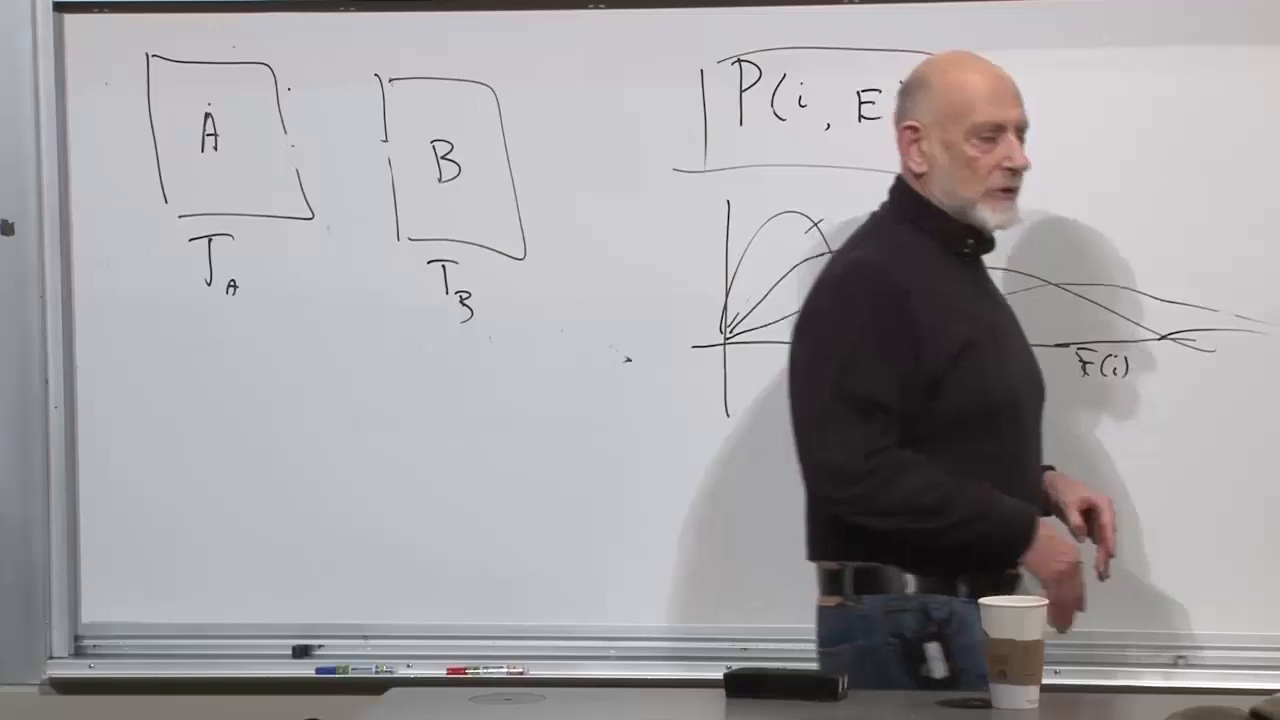
\includegraphics[width=0.88\textwidth]{lecture_02_figure_05.png}
\caption{分别制备的系统\(A\)和\(B\)，以温度\(T_A\)和\(T_B\)标记，就在考虑弱热接触之前。}
\lectureframe{00:48:55}
\end{figure}

\begin{figure}[t]
\centering
\begin{tikzpicture}[>=Stealth]
\draw[rounded corners,thick,fill=blue!6] (0,0) rectangle (2.6,2.4);
\draw[rounded corners,thick,fill=orange!8] (5.4,0) rectangle (8,2.4);
\draw[thick] (2.6,1.35) -- (5.4,1.35);
\draw[thick] (2.6,1.05) -- (5.4,1.05);
\draw[<->,very thick] (3.15,1.2) -- (4.85,1.2)
  node[midway,above] {\(\delta E\)};
\node at (1.3,1.45) {\Large \(A\)};
\node at (6.7,1.45) {\Large \(B\)};
\node at (1.3,0.65) {\(T_A,S_A,E_A\)};
\node at (6.7,0.65) {\(T_B,S_B,E_B\)};
\node at (4,0.35) {\small weak thermal contact};
\end{tikzpicture}
\caption{能量通过弱接触涨落，而组合系统保持隔离。}
\end{figure}

假设，不失一般性，
\begin{equation}
 T_B>T_A.
 \label{eq:sm2-temperature-order}
\end{equation}
经验表明\(B\)应当失去能量，而\(A\)应当获得能量。三个事实将这一预期转化为计算。

\subsection{熵的可加性}

对于两个弱耦合的子系统，其微观选择独立组合，联合可能性的数目相乘：
\[
 W_{AB}=W_AW_B.
\]
熵是对数，因此
\begin{equation}
 S_{\mathrm{tot}}=S_A+S_B.
 \label{eq:sm2-entropy-additivity}
\end{equation}
同样的结果可以直接从乘积分布的香农熵得到。

\begin{classroomqa}
\classquestion{为什么组合系统的熵会相加？}
\lecturerresponse{因为底层可能性的数目相乘，而熵取对数：
\(\log(W_AW_B)=\log W_A+\log W_B\)。弱相互作用正是允许子系统描述和这种领头可加形式的原因。
\lecturetimestamp{00:51:06--00:52:03}}
\end{classroomqa}

\subsection{第一定律和第二定律}

复合系统是孤立的，因此内部交换的能量守恒：
\begin{equation}
 dE_A+dE_B=0,
 \qquad
 dE_B=-dE_A.
 \label{eq:sm2-first-law}
\end{equation}
这就是本实验中的第一定律。

这里把第二定律当作一个公设，稍后再作更深入的说明。
当相连的两个系统向新的平衡态弛豫时，
\begin{equation}
 dS_{\mathrm{tot}}=dS_A+dS_B\geq0.
 \label{eq:sm2-second-law}
\end{equation}
严格不等式描述的是偏离平衡态的自发弛豫；
在平衡态下，对于可逆的一阶变分，等号成立。

最后，温度的定义适用于每个子系统：
\begin{equation}
 dE_A=T_A\,dS_A,
 \qquad
 dE_B=T_B\,dS_B.
 \label{eq:sm2-two-temperatures}
\end{equation}

\begin{figure}[H]
\centering
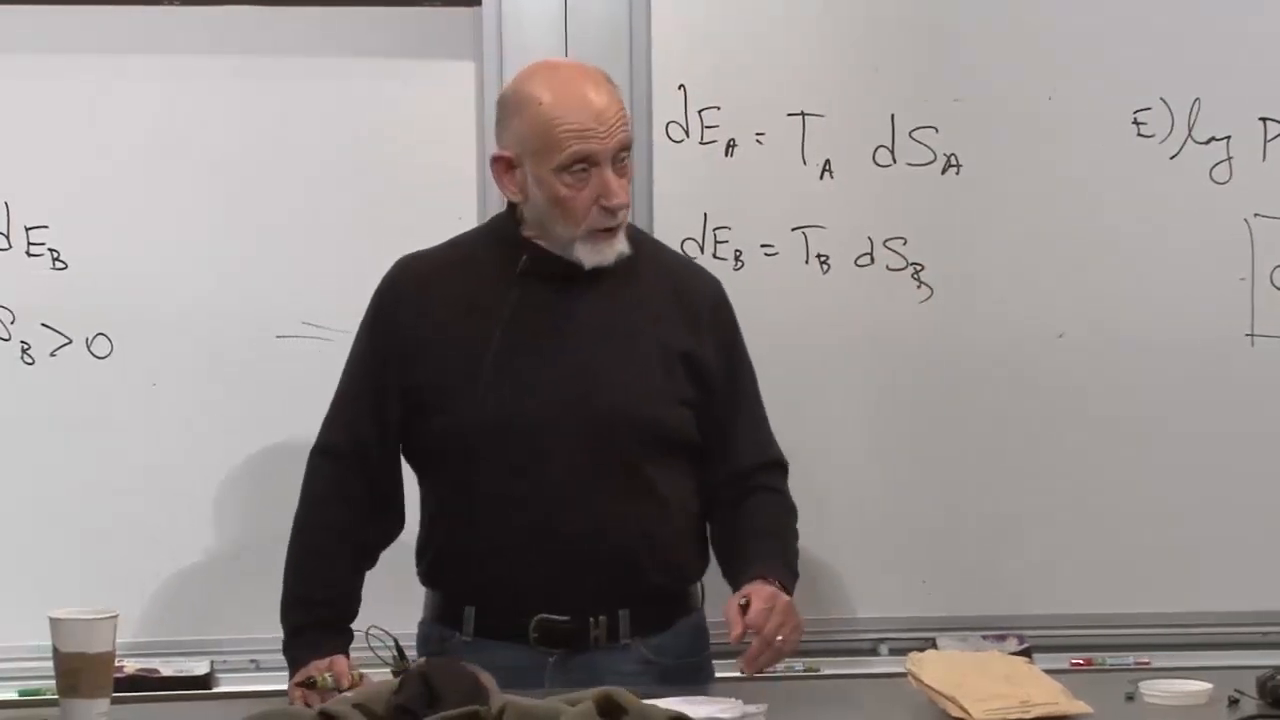
\includegraphics[width=0.88\textwidth]{lecture_02_figure_06.png}
\caption{黑板论证结束时给出的两个子系统关系式
\(dE_A=T_A\,dS_A\) 和 \(dE_B=T_B\,dS_B\)。}
\lectureframe{00:54:00}
\end{figure}

\subsection{能量流动的符号}

这些方程已经确定了净传递的方向。将
\(dS_A=dE_A/T_A\)、\(dS_B=dE_B/T_B\) 和
\eqref{eq:sm2-first-law} 代入 \eqref{eq:sm2-second-law}：
\begin{align}
 dS_{\mathrm{tot}}
 &=\frac{dE_A}{T_A}+\frac{dE_B}{T_B}\\
 &=dE_A\left(\frac{1}{T_A}-\frac{1}{T_B}\right)\geq0.
 \label{eq:sm2-flow-sign}
\end{align}
如果 \(T_B>T_A>0\)，那么
\[
 \frac{1}{T_A}-\frac{1}{T_B}>0.
\]
因此方程 \eqref{eq:sm2-flow-sign} 要求
\[
 dE_A>0,
 \qquad
 dE_B<0.
\]
较冷的系统 \(A\) 获得能量，较热的系统 \(B\) 失去能量。
当 \(T_A=T_B\) 时，一阶熵变不提供任何优先方向，微观交换相互抵消，净流动为零。于是，
抽象的导数 \(T=dE/dS\) 再现了热与冷的操作区分。
\chapter{多重度、熵与约束平衡}

\lectureoverview{一旦概率分布的各状态带有能量，它就成为一个热力学对象。我们首先把熵增与平衡化联系起来，并利用\(dE=T\,dS\)导出热流的方向。随后，我们将一个系统替换为大量复制品构成的大集合，对与每一组占据数相对应的排列方式进行计数，并证明这一多重度的对数等于\(N\)乘以熵。因此，平衡是一个受约束的最大熵问题。拉格朗日乘子提供了求解该问题所需的方法。}

\section{三个基本量}

设\(i\)标记系统可用的离散状态。就目前而言，离散性是有用的，因为它使我们能够在不引入相空间测度的情况下对状态进行计数。若状态\(i\)的概率为\(P_i\)，则
\begin{equation}
 \sum_i P_i=1.
 \label{eq:sm3-normalization}
\end{equation}
若该状态的能量为\(E_i\)，则平均能量为
\begin{equation}
 \overline E=\sum_iP_iE_i.
 \label{eq:sm3-mean-energy}
\end{equation}
\emph{平均}一词很重要。系统在任何单个微观状态中都不必具有值\(\overline E\)；它是各可能值按概率加权的平均值。

\begin{classroomqa}
\classquestion{这里概率与统计之间是否存在有用的区分？}
\lecturerresponse{概率为可能的结果提供模型，而统计通常从观测数据出发，追问能从中推断出什么。当前的计算使用的是概率分布，尽管同样的平均值自然会出现在统计数据中。课堂上这一非正式的交流对这两个词处理得比较随意，因为这一区分并不影响后续的物理。
\lecturetimestamp{00:01:39--00:02:21}}
\end{classroomqa}

该分布的熵为
\begin{equation}
 S[P]=-\sum_iP_i\log P_i.
 \label{eq:sm3-entropy}
\end{equation}
此表达式非负。每个非零概率都满足\(0<P_i\leq1\)，因此\(\log P_i\leq0\)，而当\(P_i\to0\)时，适用通常的极限值\(P_i\log P_i\to0\)。

\begin{figure}[t]
\centering
\includegraphics[width=0.88\textwidth]{lecture_03_figure_02.png}
\caption{开场的板书将熵、归一化和平均能量公式连同定性的一族平衡分布汇集在一起。}
\lectureframe{00:06:44}
\end{figure}

\section{作为一族分布的平衡}

上一讲给我们留下了一族单参数的平衡分布。人们可以用温度来标记这一族分布，但目前用平均能量\(\overline E\)来标记它更为有用。在最低可能能量处，分布集中在一个基态上：
\[
 P_i=\delta_{i0}.
\]
此时状态没有任何不确定性，且\(S=0\)。随着平衡分布扩展到更多能级上，其平均能量和熵都增大。

这是关于热学族分布的陈述，而不是关于一切可以设想出来的分布的陈述。任意一族分布可能在向更大能量移动的同时变得更窄。将要导出的平衡分布在通常的正温度区域内不会如此。沿着这一族分布，
\begin{equation}
 \frac{dS}{d\overline E}>0.
 \label{eq:sm3-positive-temperature-branch}
\end{equation}
具有有界谱的系统也可以有使该导数为负的分支。这些负温度区域是真实存在的，但在当前的论证中我们将其搁置一旁。

热平衡不仅仅意味着微观上的静止。分子继续运动、碰撞并交换能量。变得定常的是宏观描述：分布不再表现出净漂移，系统的各个分离部分不再维持净能量流。

\section{统计语言中的热力学定律}

第一定律是能量守恒。第二定律说，一个孤立宏观系统的热力学熵不会减少：
\begin{equation}
 \Delta S_{\mathrm{tot}}\geq0.
 \label{eq:sm3-second-law}
\end{equation}
等号描述的是平衡或理想的可逆变化；自发弛豫通常给出严格增加。

在概率图像中，弛豫倾向于将权重散布到我们仍然区分的那些宏观备选情形上。这一陈述需要讲座中强调的限定：我们是在\emph{粗粒化}。精确的哈密顿演化保持细粒化的相空间熵不变。宏观熵之所以增长，是因为我们不再追踪微观的关联和细节。丢失这类信息会拓宽约化描述。相反，自发的变窄则意味着我们在没有进行测量的情况下获得了微观信息。

第零定律断言系统能够达到热平衡，并且平衡具有传递性。如果\(A\)与\(B\)处于平衡，而\(B\)与\(C\)处于平衡，那么\(A\)与\(C\)处于平衡。温度提供了使这种传递性变得显然的数值：
\[
 T_A=T_B,\qquad T_B=T_C
 \quad\Longrightarrow\quad
 T_A=T_C.
\]
在非平衡时，能量从温度较高的子系统流向温度较低的子系统。当温度相等时，净流动停止。现在我们从温度的熵定义出发推导这一操作性陈述。

\section{为什么能量从热流向冷}

考虑两个弱耦合的子系统\(A\)和\(B\)。每个子系统内部都处于平衡，但它们的温度不同。选择标记使得
\begin{equation}
 T_B>T_A>0.
 \label{eq:sm3-temperature-order}
\end{equation}
在一次小交换过程中，组合能量的守恒给出
\begin{equation}
 dE_A+dE_B=0.
 \label{eq:sm3-energy-conservation}
\end{equation}
第二定律给出
\begin{equation}
 dS_A+dS_B\geq0.
 \label{eq:sm3-entropy-change}
\end{equation}
对于每个内部平衡的子系统，温度由下式定义
\begin{equation}
 dE_X=T_X\,dS_X,
 \qquad X=A,B.
 \label{eq:sm3-temperature-differential}
\end{equation}
代入\eqref{eq:sm3-energy-conservation}得到
\begin{equation}
 T_A\,dS_A+T_B\,dS_B=0,
\end{equation}
因而
\begin{equation}
 dS_B=-\frac{T_A}{T_B}\,dS_A.
 \label{eq:sm3-dsb}
\end{equation}
将此结果代入\eqref{eq:sm3-entropy-change}，
\begin{align}
 dS_{\mathrm{tot}}
 &=dS_A-\frac{T_A}{T_B}dS_A\\
 &=\frac{T_B-T_A}{T_B}\,dS_A\geq0.
 \label{eq:sm3-flow-entropy}
\end{align}
因为\(T_B-T_A>0\)且\(T_B>0\)，自发交换要求
\[
 dS_A>0.
\]
于是方程\eqref{eq:sm3-temperature-differential}给出
\begin{equation}
 dE_A=T_A\,dS_A>0,
 \qquad
 dE_B=-dE_A<0.
 \label{eq:sm3-hot-to-cold}
\end{equation}
能量已从\(B\)，即较热的子系统，流向\(A\)，即较冷的子系统。这里热量仅仅是传输中的能量。流动持续到\(T_A=T_B\)，此时一阶熵变不再偏向任何一个方向。

同样的结果可以写成一行：
\begin{equation}
 dS_{\mathrm{tot}}
 =dE_A\left(\frac{1}{T_A}-\frac{1}{T_B}\right)\geq0.
 \label{eq:sm3-compact-flow}
\end{equation}
逆温度差的符号决定了\(dE_A\)的符号。这种紧凑形式以后将自然地与正则系综相契合。

\begin{classroomqa}
\audiencequestion{这个论证是否假设\(A\)和\(B\)各自已经处于内部平衡？}
\lecturerresponse{是的。指定单一的\(T_A\)或\(T_B\)就作出了这一假设。如果某个子系统内部未达到平衡，就把它分成更小的区域，并在能够定义温度的每个局部应用该论证。整体的弛豫则由这些区域之间的交换组合而成。
\lecturetimestamp{00:24:38--00:25:22}}
\end{classroomqa}

\section{什么算作一个态？}

在询问平衡概率之前，我们必须知道标记\(i\)意味着什么。微观态是底层物理定律所允许的对系统的最完整描述。在经典力学中，人们设想所有粒子的位置和动量。在量子力学中，态则是一个完整的量子态；不确定性原理阻止同时精确指定每一个经典位置和动量。

对于有限盒子中的量子系统，相关的态计数可以是离散的。经典统计力学在适当的极限下出现，此时对密集分布的量子态求和变为相空间积分。这一取极限的过程还引入了使连续熵无量纲化所需的相空间元胞；它并非仅仅通过把求和号换成积分号就能得到。

\begin{classroomqa}
\audiencequestion{对于气体，是否应当把一个态想象为每个分子的位置和动量？}
\lecturerresponse{这是正确的经典图像。更一般地说，一个态意味着在物理定律约束下原则上能够知道的关于系统的一切。量子力学改变了这种最大描述的形式，并使有限体积下的计数变为离散的。从量子求和恢复经典积分是一个真正的取极限论证，而不是一行替换。
\lecturetimestamp{00:25:31--00:27:38}}
\end{classroomqa}

\section{由复制品构成的热浴}

现在无法回避这个困难的问题：在平衡建立之后，什么决定了\(P_i\)？

将子系统与一个非常大的热浴接触。能量可以来回传递，但热浴具有如此多的自由度，以至于少量能量的转移几乎不改变其温度。一种特别方便的热浴由子系统自身的许多弱耦合复制品组成。一个复制品是所研究的系统；其余复制品构成它的环境。

这种构造常常对应一个真实的宏观系统。将一个大体上近乎均匀的物体分成许多相似的元胞。每个元胞是一个子系统，而其余元胞充当它的热浴。用\(N\)表示复制品的总数。课堂演示使用九个复制品和三种有颜色的态标记，但计数与这些具体数字无关。

设\(n_i\)为处于态\(i\)的复制品数目。这些就是\emph{占据数}。可能的能级可以有无限多个，但在有限总能量下，大多数非常高的能级的占据数可以忽略或为零。

第一个约束条件就是复制品的数目：
\begin{equation}
 \sum_i n_i=N.
 \label{eq:sm3-number-constraint}
\end{equation}
第二个是总能量：
\begin{equation}
 \sum_i n_iE_i=N\overline E.
 \label{eq:sm3-total-energy-constraint}
\end{equation}
右端是广延量。若复制品的数目加倍而它们的统计状态保持不变，则总能量加倍，而每个复制品的平均能量仍为\(\overline E\)。

\begin{classroomqa}
\audiencequestion{复制品构造是否也必须满足一个能量约束？}
\lecturerresponse{是的。占据数之和必须等于\(N\)，而它们的能量加权和必须等于固定的总能量\(N\overline E\)。这正是之后将限制熵最大值的两个约束条件。
\lecturetimestamp{00:37:12--00:39:54}}
\end{classroomqa}

随机选取的一个复制品占据态\(i\)的概率就是它的相对频率：
\begin{equation}
 P_i=\frac{n_i}{N},
 \qquad
 n_i=NP_i.
 \label{eq:sm3-frequency-probability}
\end{equation}

\begin{figure}[t]
\centering
\includegraphics[width=0.82\textwidth]{lecture_03_figure_03.png}
\caption{能级图像以及将概率等同于占据分数\(P_i=n_i/N\)。}
\lectureframe{00:41:40}
\end{figure}

\begin{classroomqa}
\audiencequestion{黑板上的记号\(N(i)\)是否意在区别于\(n_i\)？}
\lecturerresponse{不是。两者都表示态\(i\)的占据数。我们一致地使用\(n_i\)，而将大写\(N\)保留给复制品的总数。
\lecturetimestamp{00:41:28--00:41:33}}
\end{classroomqa}

将\eqref{eq:sm3-number-constraint}和\eqref{eq:sm3-total-energy-constraint}除以\(N\)，就重新得到概率约束条件：
\begin{equation}
 \sum_iP_i=1,
 \qquad
 \sum_iP_iE_i=\overline E.
 \label{eq:sm3-probability-constraints}
\end{equation}
因此，系综频率解释重现了我们开始时所用的方程。

\section{一种占据模式的 multiplicity}

固定一组占据数\(\{n_i\}\)。将\(N\)个可区分复制品分配到各态，有多少种分配方式恰好实现该组占据数？答案是多项式系数
\begin{equation}
 C(\{n_i\})=\frac{N!}{\prod_i n_i!}.
 \label{eq:sm3-multiplicity}
\end{equation}
为看清分母，首先将全部\(N\)个带标记的复制品排成\(N!\)种顺序。对占据同一态的\(n_i\)个复制品进行置换不会产生新的占据分配，因此对每个态都要除以\(n_i!\)。

\begin{figure}[t]
\centering
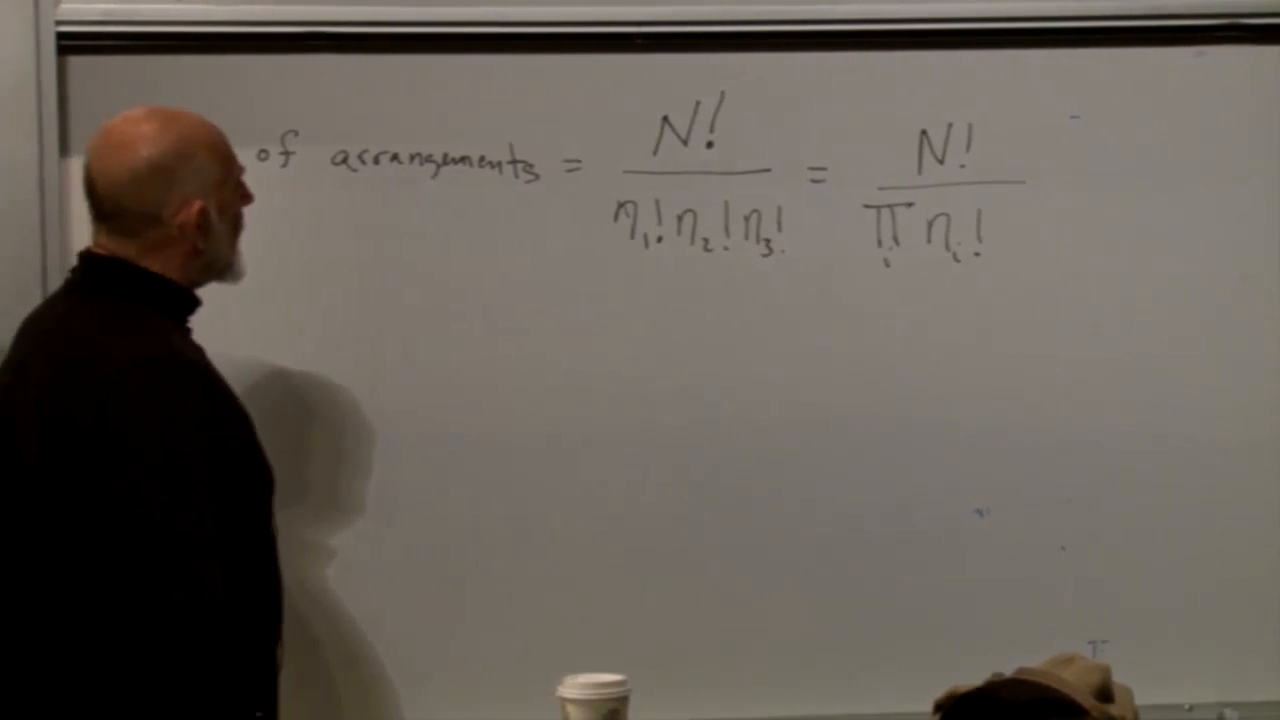
\includegraphics[width=0.88\textwidth]{lecture_03_figure_04.png}
\caption{黑板上写出的多项式 multiplicity
\(C=N!/\prod_i n_i!\)。}
\lectureframe{00:46:55}
\end{figure}

未被占据的能级不会造成问题，因为\(0!=1\)。如果所有复制品都占据一个态，那么
\[
 C=\frac{N!}{N!}=1,
\]
正如预期。如果三个复制品占据三个不同的指定态，那么
\[
 C=\frac{3!}{1!\,1!\,1!}=6.
\]
当两个复制品占据两个指定态时，该公式给出两种分配：交换哪个带标记的复制品占据哪个态。

\begin{classroomqa}
\audiencequestion{是否可能有不止一组占据数满足这两个约束条件？}
\lecturerresponse{通常有许多组都满足。方程
\eqref{eq:sm3-multiplicity}首先对某一固定组\(\{n_i\}\)计算排列数，此时尚未判定它是否满足约束条件。下一阶段则比较所有与约束相容的组，并找出其中 multiplicity 最大的那一组。
\lecturetimestamp{00:48:07--00:48:43}}
\end{classroomqa}

统计假设是：与孤立装置相容的微观分配被对称地对待。因此，由更多分配实现的一种宏观占据模式就更可能。对于大的\(N\)，关于分数\(n_i/N\)的分布会变得尖锐地集中。平衡分数就是在\eqref{eq:sm3-number-constraint}和
\eqref{eq:sm3-total-energy-constraint}的约束下使\(C\)最大的那些值。

\section{斯特林近似}

早在\(N\)达到宏观值之前，阶乘就已经变得极其巨大，因此我们改用它们的对数。从
\begin{equation}
 \log N!=\sum_{x=1}^{N}\log x.
 \label{eq:sm3-log-factorial-sum}
\end{equation}
开始。对于大的\(N\)，该和式可用\(\log x\)下方的面积来近似：
\begin{align}
 \log N!
 &\simeq\int_1^N\log x\,dx\\
 &=\left[x\log x-x\right]_1^N\\
 &=N\log N-N+1.
 \label{eq:sm3-stirling-integral}
\end{align}
原函数立即可由
\[
 \frac{d}{dx}(x\log x-x)=\log x.
\]
得到。在领先的广延阶下，可以略去加性常数：
\begin{equation}
 \log N!\simeq N\log N-N.
 \label{eq:sm3-stirling-log}
\end{equation}
取指数便得到讲座中所用的简化形式，
\begin{equation}
 N!\simeq N^N e^{-N}.
 \label{eq:sm3-stirling-simple}
\end{equation}

\begin{figure}[t]
\centering
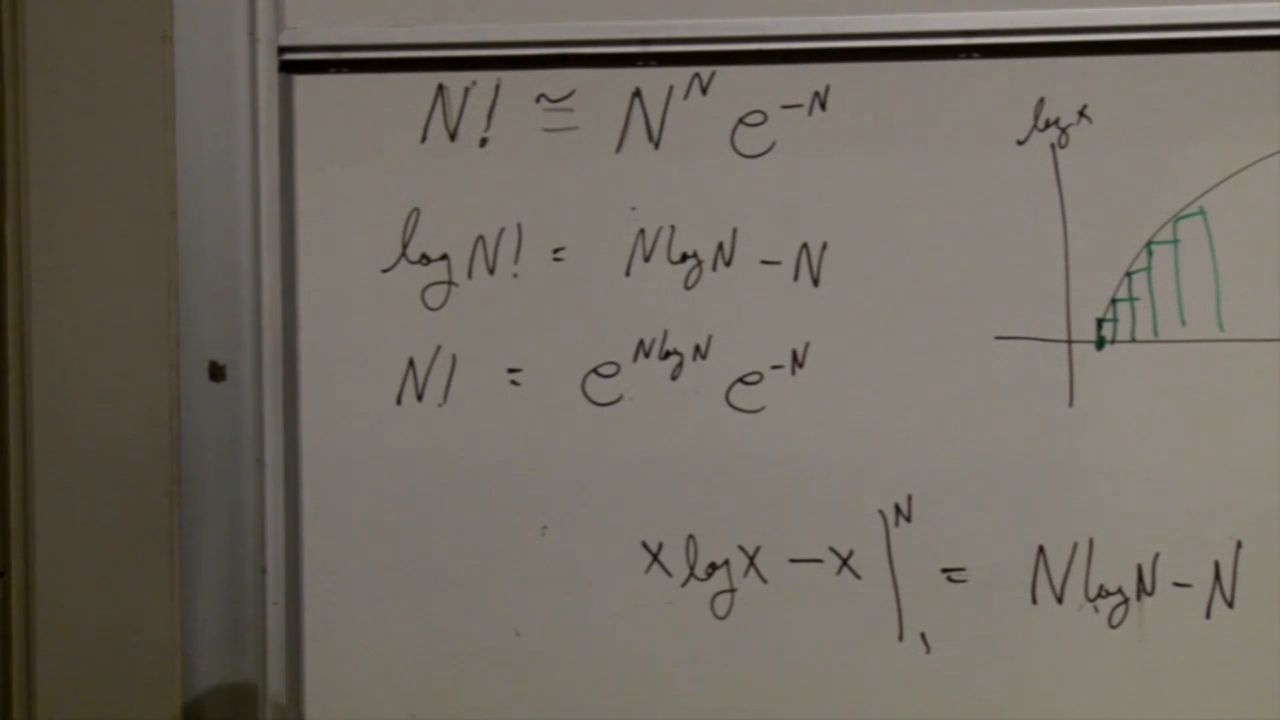
\includegraphics[width=0.88\textwidth]{lecture_03_figure_05.png}
\caption{领先的斯特林近似，以及通过将\(\log x\)的和式替换为积分而得到的推导。}
\lectureframe{01:03:45}
\end{figure}

\begin{classroomqa}
\audiencequestion{在下限处计算\(x\log x-x\)是否会留下一个额外的\(+1\)？}
\lecturerresponse{是的。方程\eqref{eq:sm3-stirling-integral}包含那个常数。当\(N\to\infty\)时，与正比于\(N\)的项相比，它可以忽略不计，这就是领先公式略去它的原因。和式本身必须从\(x=1\)开始；\(\log0\)没有定义。
\lecturetimestamp{01:04:12--01:04:35}}
\end{classroomqa}

\begin{classroomqa}
\audiencequestion{是否还缺少一个正比于\(\sqrt{N}\)的因子？}
\lecturerresponse{是的。更精确的渐近公式是
\[
 N!\sim\sqrt{2\pi N}\left(\frac{N}{e}\right)^N.
\]
它的对数只增加\(\tfrac12\log(2\pi N)\)，与\(N\log N-N\)相比是次广延的。它对于精确的有限\(N\)概率很重要，但对于宏观系统的领先熵计算并不重要。
\lecturetimestamp{01:04:35--01:05:40}}
\end{classroomqa}

在\eqref{eq:sm3-multiplicity}的分母中，也必须谨慎使用斯特林近似。在热力学极限下，具有非零极限概率的状态满足\(n_i=NP_i\)，因此它们的占据数随\(N\)增长。占据数极小或趋于零的状态可以通过有限能量截断来处理，然后再通过取极限恢复。被省略的次领头项不影响领头的广延熵。

\section{多重性的对数即熵}

对分子以及所有宏观上被占据的分母因子应用\eqref{eq:sm3-stirling-simple}：
\begin{equation}
 C\simeq
 \frac{N^Ne^{-N}}
 {\prod_i n_i^{\,n_i}e^{-n_i}}.
 \label{eq:sm3-c-stirling}
\end{equation}
由于\(\sum_i n_i=N\)，领头的指数因子相消：
\begin{equation}
 C\simeq\frac{N^N}{\prod_i n_i^{\,n_i}}.
 \label{eq:sm3-c-leading}
\end{equation}
对对数求极大比对乘积求极大更容易，而对数是单调的，所以两个极大值出现在同一占据模式上：
\begin{equation}
 \log C=N\log N-\sum_i n_i\log n_i.
 \label{eq:sm3-logc-occupations}
\end{equation}
现在代入\(n_i=NP_i\)：
\begin{align}
 \log C
 &=N\log N-\sum_iNP_i\log(NP_i)\\
 &=N\log N-N\sum_iP_i\log N
   -N\sum_iP_i\log P_i\\
 &=-N\sum_iP_i\log P_i,
 \label{eq:sm3-logc-entropy-derivation}
\end{align}
其中归一化使两个\(N\log N\)项相消。因此，在\(N\)的领头阶下，
\begin{equation}
 \boxed{\log C=NS}.
 \label{eq:sm3-logc-ns}
\end{equation}

\begin{figure}[t]
\centering
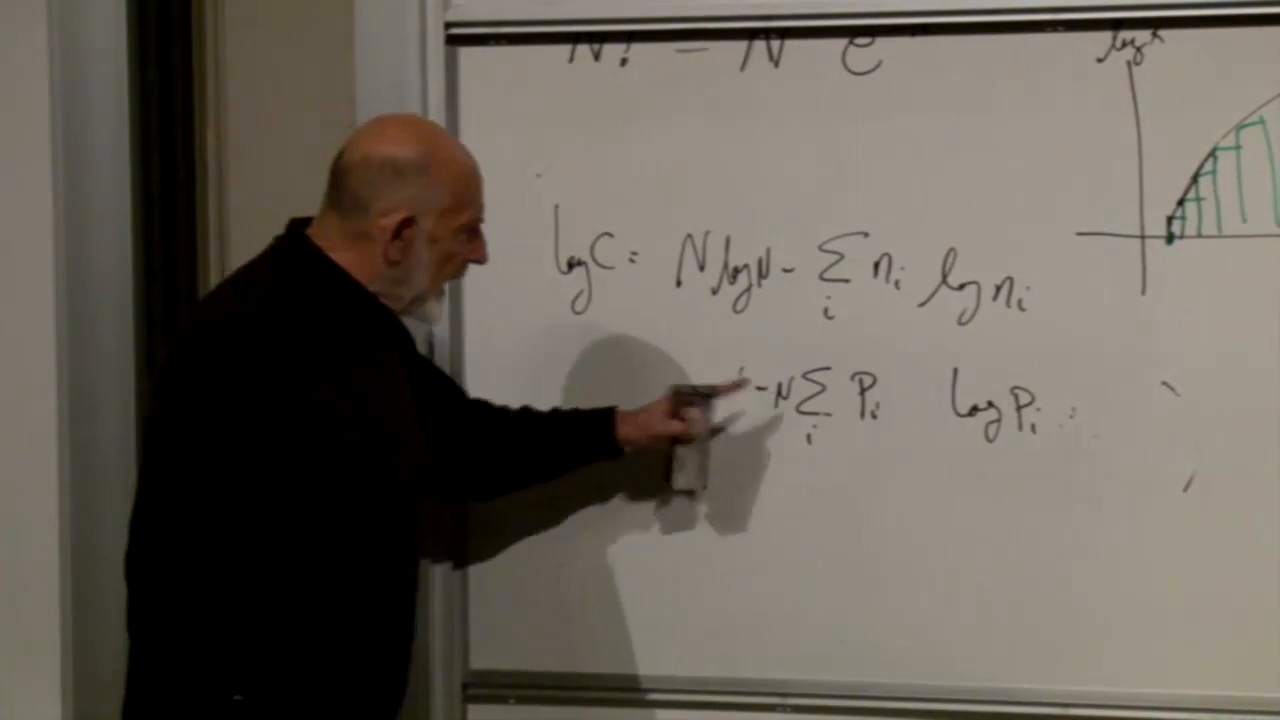
\includegraphics[width=0.88\textwidth]{lecture_03_figure_06.png}
\caption{将\(\log C=N\log N-\sum_i n_i\log n_i\)与\(-N\sum_iP_i\log P_i=NS\)联系起来的板书计算。}
\lectureframe{01:16:10}
\end{figure}

这一关系是本章的概念核心。熵并非强加于计数问题之上的一个无关量。它是每个复本的 multiplicity，以对数方式度量。因此，在领头阶下，最大化微观排列数等同于最大化一个复本的熵。

\begin{classroomqa}
\audiencequestion{当所有占据数都相等时，多重性难道不是最大吗？}
\lecturerresponse{当没有状态被区分，且只在一个有限状态集上施加\(\sum_i n_i=N\)时，它是均匀的。固定能量的约束改变了答案，因为\(E_i\)的值不同。相等的占据数一般无法产生指定的平均能量。
\lecturetimestamp{01:17:07--01:18:20}}
\end{classroomqa}

\begin{classroomqa}
\audiencequestion{大写\(N\)很大，但为什么可以对分母中的每一个\(n_i\)都应用斯特林近似？}
\lecturerresponse{对于每个具有非零极限概率的状态，\(n_i=NP_i\)正比于\(N\)增长。可以先保留一个有限能量范围，在其中取大\(N\)极限，然后再扩大该范围。稀疏的尾部状态需要单独的有限修正，但它们不改变领头的广延熵。
\lecturetimestamp{01:18:23--01:19:28}}
\end{classroomqa}

\begin{classroomqa}
\audiencequestion{这个大的\(N\)近似就是前面所说的粗粒化吗？}
\lecturerresponse{不是。热力学极限控制的是大占据数和渐近计数。粗粒化是微观分辨率的丢失或有意丢弃。它们是不同的操作，尽管在宏观统计力学中两者都经常被使用。
\lecturetimestamp{01:19:29--01:19:46}}
\end{classroomqa}

\begin{classroomqa}
\audiencequestion{既然\(\log C=N\log N-\sum_i n_i\log n_i\)，第二项难道不应该被最小化而不是最大化吗？}
\lecturerresponse{是的；在\(N\)固定的情况下，最大化\(\log C\)等价于最小化\(\sum_i n_i\log n_i\)。代入\(n_i=NP_i\)后，固定的\(N\log N\)项相消，剩下的就是\(-N\sum_iP_i\log P_i=NS\)。因此，同一操作更自然地描述为最大化正熵\(S\)。
\lecturetimestamp{01:19:48--01:20:55}}
\end{classroomqa}

\begin{classroomqa}
\audiencequestion{为什么不直接利用对称性令所有\(n_i\)相等，从而立即完成论证？}
\lecturerresponse{这种捷径忽略了能量标签。归一化约束对称地对待各状态，但\(\sum_iP_iE_i=\overline E\)并非如此：不同能量的状态贡献不同。能量约束正是非均匀平衡分布进入之处。
\lecturetimestamp{01:21:15--01:21:41}}
\end{classroomqa}

\section{最大熵问题}

现在我们可以毫无歧义地陈述统计力学规则。改变概率\(P_i\)并最大化
\begin{equation}
 S[P]=-\sum_iP_i\log P_i
 \label{eq:sm3-maximize-entropy}
\end{equation}
受约束于
\begin{equation}
 \sum_iP_i=1,
 \qquad
 \sum_iP_iE_i=\overline E.
 \label{eq:sm3-maxent-constraints}
\end{equation}
使该式最大的概率给出大复本系综中尖锐偏好的占据分数。占据数会涨落，但它们的相对偏差随\(N\)增大而缩小，因此比值\(n_i/N\)成为定义良好的热力学概率。

\begin{classroomqa}
\audiencequestion{\(E_i\)是固定的状态能量，而约束使用的是另外给定的总能量吗？}
\lecturerresponse{是的。谱\(\{E_i\}\)属于子系统。完整的复本集合具有固定的总能量，但能量不断在复本之间转移。将该总量除以\(N\)固定的是一个复本的平均能量\(\overline E\)，而不是它在每个微观实现中的能量。
\lecturetimestamp{01:26:12--01:27:07}}
\end{classroomqa}

这个问题容易陈述，但尚未解决。它是一个带有两个约束的极值问题，因此还需要一个数学工具。

\section{拉格朗日乘子}

对于无约束函数 \(F(x_1,x_2,\ldots)\)，驻点满足
\begin{equation}
 \frac{\partial F}{\partial x_i}=0
 \qquad\text{for every }i.
 \label{eq:sm3-unconstrained-stationary}
\end{equation}
现在再要求
\begin{equation}
 G(x_1,x_2,\ldots)=0.
 \label{eq:sm3-one-constraint}
\end{equation}

\begin{classroomqa}
\audiencequestion{如果图中坐标是 \(x\)
和 \(y\)，那么 \(x\) 是什么意思？}
\lecturerresponse{这里 \(x\) 是整个坐标向量
\((x_1,x_2,\ldots)\) 的简写。在二维图中，它的分量就是
\(x\) 和 \(y\)。之后这些分量将是概率
\(P_1,P_2,\ldots\)。
\lecturetimestamp{01:30:12--01:30:20}}
\end{classroomqa}

从几何上看，等值线 \(F=\text{constant}\) 构成一幅等高线图，
而 \(G=0\) 是系统被允许在其上运动的曲线。约束极值出现在
\(F\) 的某条等值线与约束曲线相切之处。在该点，梯度平行：
\begin{equation}
 \nabla F=-\lambda\nabla G
 \label{eq:sm3-parallel-gradients}
\end{equation}
其中 \(\lambda\) 是某个数。

\begin{figure}[t]
\centering
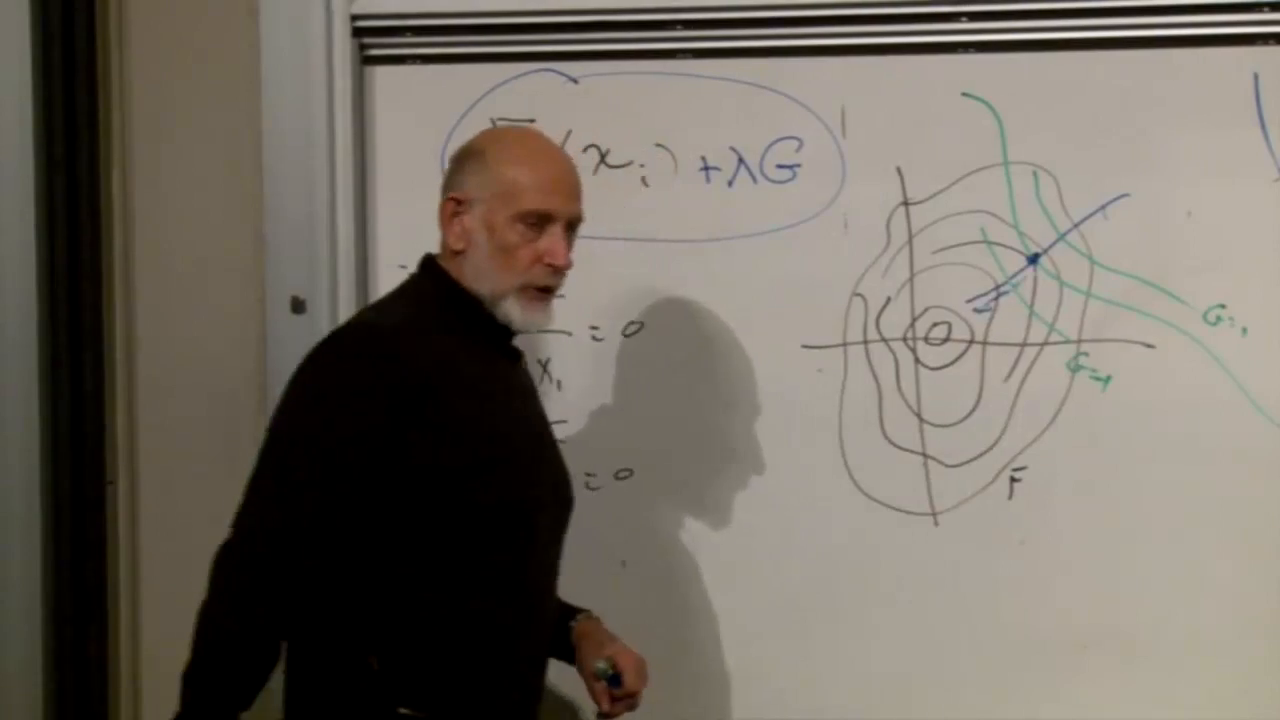
\includegraphics[width=0.88\textwidth]{lecture_03_figure_07.png}
\caption{黑板上的等高线几何以及增广函数
\(F'=F+\lambda G\)。约束极值出现在相切处。}
\lectureframe{01:37:10}
\end{figure}

方程 \eqref{eq:sm3-parallel-gradients} 可以通过定义
增广函数
\begin{equation}
 F'=F+\lambda G
 \label{eq:sm3-augmented-function}
\end{equation}
并要求普通驻点条件得到：
\begin{equation}
 \frac{\partial F'}{\partial x_i}=0.
 \label{eq:sm3-augmented-stationarity}
\end{equation}
乘子 \(\lambda\) 起初未知。这并不会使系统欠定，因为原约束 \(G=0\) 提供了一个
额外方程。

\begin{classroomqa}
\classquestion{为什么加上一个正比于 \(G\) 的项会使
约束点成为驻点？}
\lecturerresponse{在约束极值处，沿 \(G=0\) 的切向运动
已经不产生 \(F\) 的一阶变化。唯一剩余的斜率垂直于约束。由于 \(\nabla G\) 指向同一个法向，
适当的 \(\lambda\) 会将其抵消：
\(\nabla F+\lambda\nabla G=0\)。
\lecturetimestamp{01:35:06--01:35:32}}
\end{classroomqa}

\section{一个二变量例子}

最小化
\begin{equation}
 F(x,y)=\frac{x^2+y^2}{2}
 \label{eq:sm3-example-f}
\end{equation}
受约束于
\begin{equation}
 x+y=1.
 \label{eq:sm3-example-constraint}
\end{equation}
将约束写成 \(G=x+y-1=0\) 并构造
\begin{equation}
 F'=\frac{x^2+y^2}{2}+\lambda(x+y-1).
 \label{eq:sm3-example-augmented}
\end{equation}
驻点方程为
\begin{align}
 \frac{\partial F'}{\partial x}&=x+\lambda=0,\\
 \frac{\partial F'}{\partial y}&=y+\lambda=0.
 \label{eq:sm3-example-derivatives}
\end{align}
因此 \(x=y=-\lambda\)。剩下的方程就是约束，
\[
 x+y=-2\lambda=1,
\]
所以
\begin{equation}
 \lambda=-\frac12,
 \qquad
 x=y=\frac12.
 \label{eq:sm3-example-solution}
\end{equation}
点 \((1/2,1/2)\) 是以原点为圆心的最小圆与直线 \(x+y=1\) 相切之处。

\begin{figure}[t]
\centering
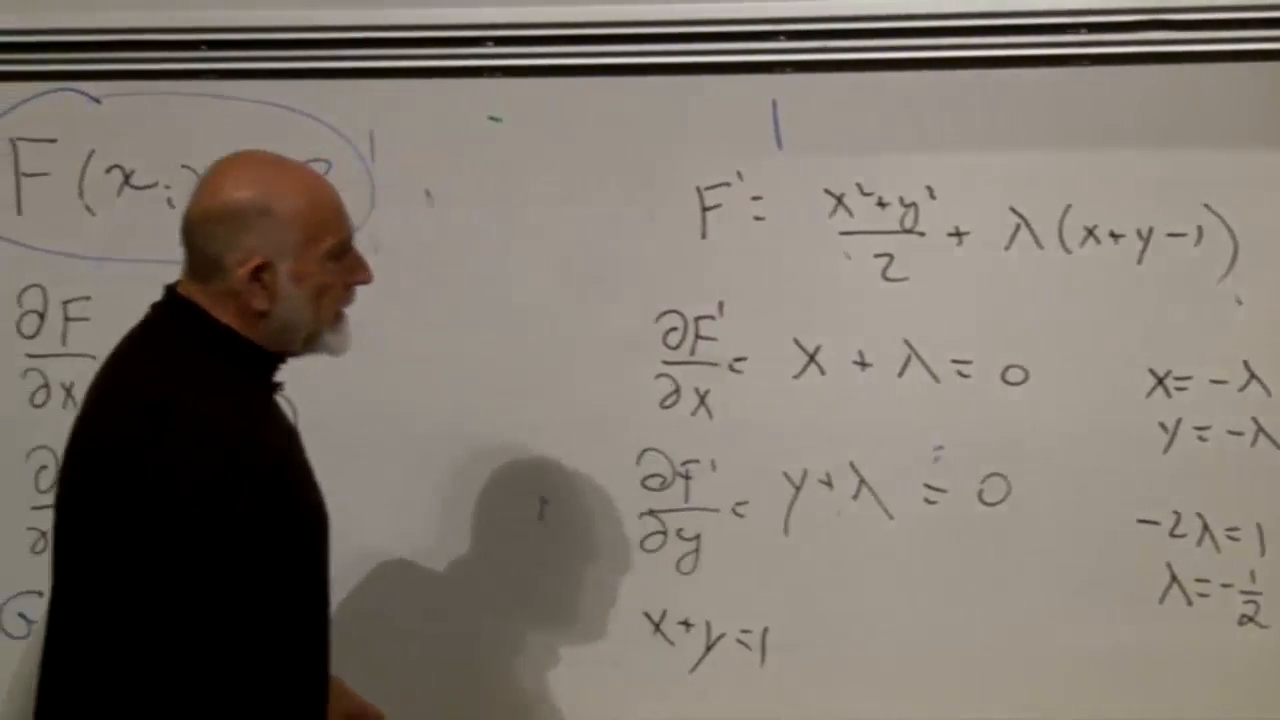
\includegraphics[width=0.88\textwidth]{lecture_03_figure_08.png}
\caption{为最小化 \((x^2+y^2)/2\) 且受约束于 \(x+y=1\) 而完成的拉格朗日乘子计算。}
\lectureframe{01:44:10}
\end{figure}

有多个约束时，为每个约束引入一个乘子：
\begin{equation}
 F'=F+\lambda_1G_1+\lambda_2G_2+\cdots.
 \label{eq:sm3-many-multipliers}
\end{equation}
然后求解
\begin{equation}
 \begin{aligned}
 \frac{\partial F'}{\partial x_i}&=0
 &&\text{for every }i,\\
 G_a&=0
 &&\text{for every constraint }a.
 \end{aligned}
 \label{eq:sm3-many-equations}
\end{equation}
本讲提出一个刻意人为的练习题：在施加两个独立线性约束（例如 \(x+y=1\) 和 \(z+x=1\)）的同时，求 \(x,y,z\) 的二次函数的极值。其目的不是那个具体答案，而是这条规则：每个约束都同时带来一个乘子和一个方程。

\section{为下一讲准备好的问题}

对于统计力学，坐标是概率
\(\{P_i\}\)，要最大化的函数是熵，约束是归一化和固定平均能量。定义
\begin{align}
 S[P]&=-\sum_iP_i\log P_i,\\
 G_1[P]&=\sum_iP_i-1,\\
 G_2[P]&=\sum_iP_iE_i-\overline E.
 \label{eq:sm3-final-functions}
\end{align}
因此增广熵可以写成
\begin{equation}
 \Phi[P]
 =S[P]+\alpha G_1[P]+\beta G_2[P].
 \label{eq:sm3-final-augmented}
\end{equation}
要求解的方程是
\begin{equation}
 \frac{\partial\Phi}{\partial P_i}=0
 \quad\text{for every }i,
 \qquad
 G_1=0,
 \qquad
 G_2=0.
 \label{eq:sm3-final-problem}
\end{equation}

\begin{figure}[H]
\centering
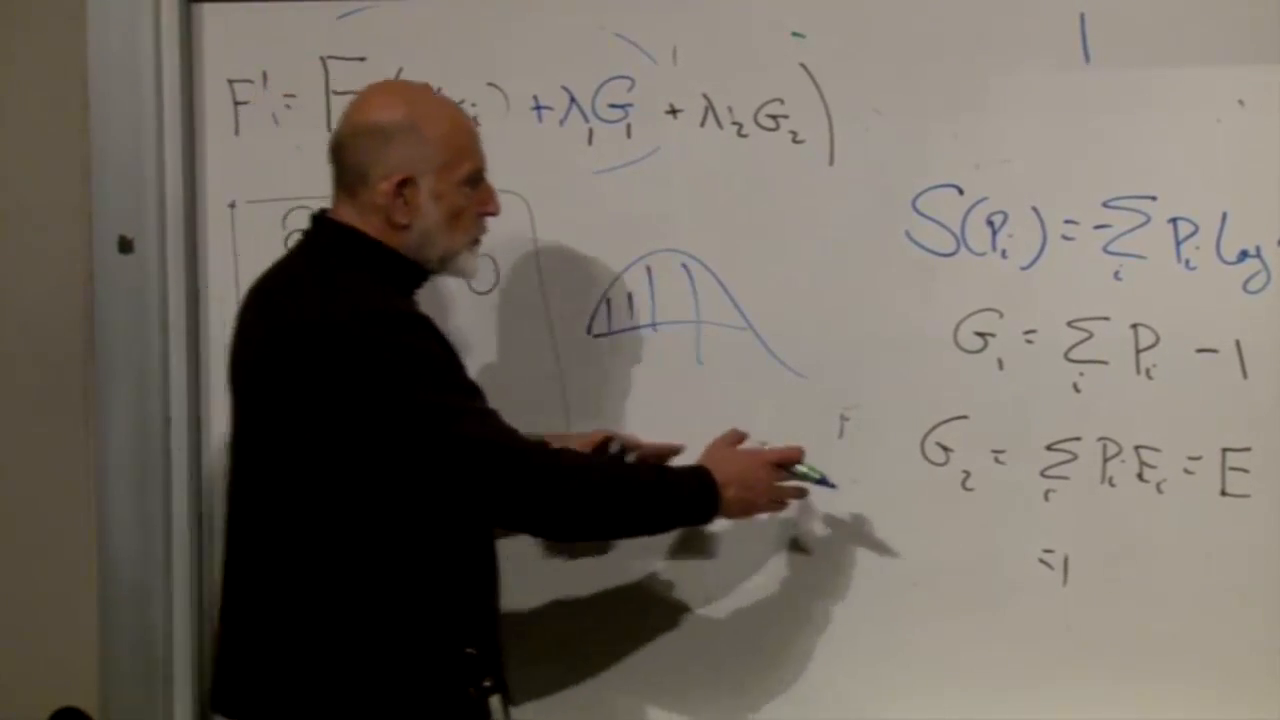
\includegraphics[width=0.88\textwidth]{lecture_03_figure_09.png}
\caption{收尾板书：作为概率函数的熵，连同归一化和固定平均能量。}
\lectureframe{01:53:05}
\end{figure}

至此，问题已经完全提出。求解
\eqref{eq:sm3-final-problem} 会给出平衡分布。与能量共轭的乘子将成为逆温度
\(\beta=1/T\)，具体取决于 \eqref{eq:sm3-final-augmented} 中所选的符号约定。下一讲将进行该微分运算并得到玻尔兹曼权重。

\chapter{玻尔兹曼权重、配分函数与理想气体}

\lectureoverview{我们通过在固定归一化和固定平均能量的条件下最大化熵，推导出平衡概率分布。随后，配分函数通过微分给出平均能量、熵和温度。理想气体提供了第一个完整例子，接着是引力推广以及能量涨落的预告。}

\section{约束熵问题}

从大量\(\mathcal N\)个相同、相互作用极弱的同一子系统的复本开始。若\(n_i\)个复本占据第\(i\)个态，则
\begin{equation}
 p_i=\frac{n_i}{\mathcal N},
 \qquad
 \sum_i p_i=1.
 \label{eq:sm4-occupation-probability}
\end{equation}
上一讲的多项式计数给出每个复本的熵，
\begin{equation}
 S[p]=-\sum_i p_i\log p_i.
 \label{eq:sm4-entropy}
\end{equation}
值得将其视为所有变量\(p_1,p_2,\ldots\)的普通函数。正是其简单的可加形式使计算成为可能。

复本集合具有固定的总能量\(\mathcal N E\)，其中\(E\)是每个复本的平均能量。因此第二个约束为
\begin{equation}
 \sum_i p_iE_i=E.
 \label{eq:sm4-energy-constraint}
\end{equation}
能级\(E_i\)属于该子系统；右侧的数\(E\)是它们的概率加权平均值。在\eqref{eq:sm4-occupation-probability}和\eqref{eq:sm4-energy-constraint}的约束下最大化\eqref{eq:sm4-entropy}，选出压倒性最可能的占据分数。

为方便起见，最小化\(-S=\sum_i p_i\log p_i\)。为每个约束引入一个拉格朗日乘子：
\begin{equation}
 \begin{aligned}
 \Phi[p;\alpha,\beta]
 &=\sum_i p_i\log p_i\\
 &\quad+\alpha\left(\sum_i p_i-1\right)\\
 &\quad+\beta\left(\sum_i p_iE_i-E\right).
 \end{aligned}
 \label{eq:sm4-augmented-functional}
\end{equation}
名称\(\alpha\)和\(\beta\)尚不是物理假设。在此阶段，它们只是为强制施加两个约束所需的两个数。

\begin{classroomqa}
\audiencequestion{增广函数也是\(\alpha\)和\(\beta\)的函数吗？}
\lecturerresponse{是的。对\(\alpha\)和\(\beta\)变分可恢复这两个约束。然而，对于当前的计算，我们保持这些乘子固定，并对概率\(p_i\)变分。它们的值随后由归一化和给定的平均能量确定。
\lecturetimestamp{00:09:32--00:09:49}}
\end{classroomqa}

\begin{figure}[t]
\centering
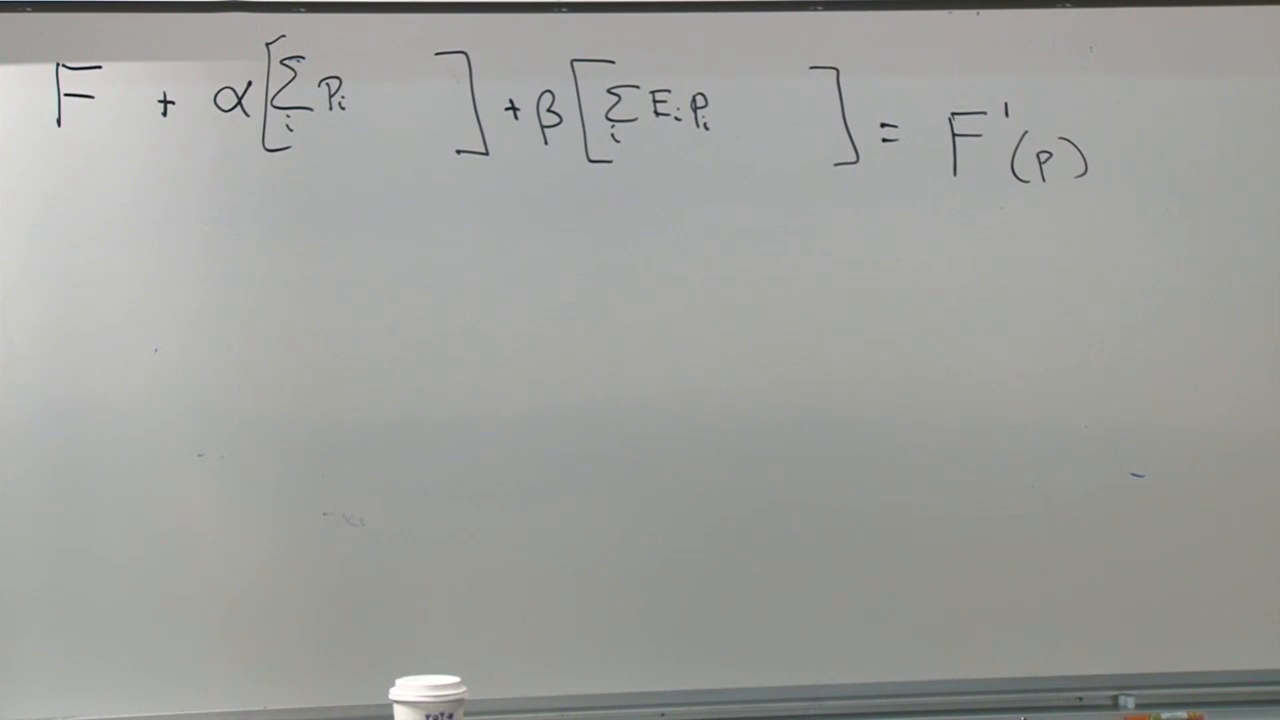
\includegraphics[width=0.92\textwidth]{lecture_04_figure_02.png}
\caption{在概率变分下为常数的项被略去后的增广熵泛函。}
\lectureframe{00:10:56}
\end{figure}

对某个概率求导时，项\(-\alpha\)和\(-\beta E\)不贡献任何东西。这就是黑板上可见的简写泛函。它们仍然是\eqref{eq:sm4-augmented-functional}的一部分；只是对这个特定的导数而言变得无关紧要。

\section{玻尔兹曼分布}

任选一个概率。本讲选择\(p_7\)，部分是因为\(1\)看起来太特殊，而\(7\)是个幸运数字。这个选择无关紧要。所需的微积分仅为
\begin{equation}
 \frac{d}{dp_i}\bigl(p_i\log p_i\bigr)=\log p_i+1.
\end{equation}
因此
\begin{equation}
 \frac{\partial\Phi}{\partial p_i}
 =\log p_i+1+\alpha+\beta E_i=0.
 \label{eq:sm4-stationarity}
\end{equation}
解出\(p_i\)，
\begin{align}
 \log p_i&=-(1+\alpha)-\beta E_i,\\
 p_i&=e^{-(1+\alpha)}e^{-\beta E_i}.
\end{align}
第一个因子与态标号无关。将其写为\(1/Z\)：
\begin{equation}
 p_i=\frac{e^{-\beta E_i}}{Z}.
 \label{eq:sm4-boltzmann-weight}
\end{equation}

这是第一个突如其来的收获。一个常规的约束导数产生了指数定律。相对概率满足
\begin{equation}
 \frac{p_i}{p_j}=e^{-\beta(E_i-E_j)}.
 \label{eq:sm4-relative-weight}
\end{equation}
乘子\(\beta\)控制概率随能量下降的快慢。大的正\(\beta\)使分布集中在最低能级附近；小的正\(\beta\)将可观的权重散布到能谱中更高的位置。我们已经可以看出，改变\(\beta\)会改变平均能量，尽管它与逆温度的等同仍有待证明。

\section{归一化与配分函数}

归一化确定了与态无关的因子：
\begin{equation}
 1=\sum_i p_i
 =\frac{1}{Z}\sum_i e^{-\beta E_i},
\end{equation}
所以
\begin{equation}
 Z(\beta)=\sum_i e^{-\beta E_i}.
 \label{eq:sm4-partition-function}
\end{equation}
这就是正则配分函数。它最初作为归一化常数出现，但这一描述严重低估了它的作用。一旦\(Z(\beta)\)已知，热力学量便可由其导数得到。

\eqref{eq:sm4-partition-function}中的能级是输入量。它们来自系统的力学以及固定的外部条件：盒子的体积和形状、磁场或电场，以及任何其他控制参数。改变控制参数会改变能谱，从而改变\(Z\)。对于当前的计算，这些参数以及集合\(\{E_i\}\)都保持固定。

\begin{classroomqa}
\audiencequestion{指数草图的坐标轴究竟代表什么？纵坐标是某个特定的\(p_i\)吗？}
\lecturerresponse{所绘制的高度是赋予某个能级的概率，而水平方向的排序既可以读作态标号\(i\)，也可以更物理地读作能量\(E_i\)。每个态都有固定的能量。大的\(\beta\)使概率随该能量急剧下降；在\(\beta=0\)附近，权重在可及能级上几乎平坦。
\lecturetimestamp{00:19:39--00:20:09}}
\end{classroomqa}

\section{隐藏在配分函数中的平均能量}

第二个约束条件确定\(\beta\)：
\begin{equation}
 E=\sum_i p_iE_i
 =\frac{1}{Z}\sum_i E_i e^{-\beta E_i}.
 \label{eq:sm4-mean-energy}
\end{equation}
与其重新计算这个加权求和，不如对
\eqref{eq:sm4-partition-function}求导：
\begin{equation}
 \frac{dZ}{d\beta}
 =-\sum_i E_i e^{-\beta E_i}.
\end{equation}
与\eqref{eq:sm4-mean-energy}比较可得
\begin{equation}
 E(\beta)
 =-\frac{1}{Z}\frac{dZ}{d\beta}
 =-\frac{d\log Z}{d\beta}.
 \label{eq:sm4-energy-logz}
\end{equation}
取自然对数，因为它的导数正好给出因子
\(1/Z\)。

\begin{figure}[t]
\centering
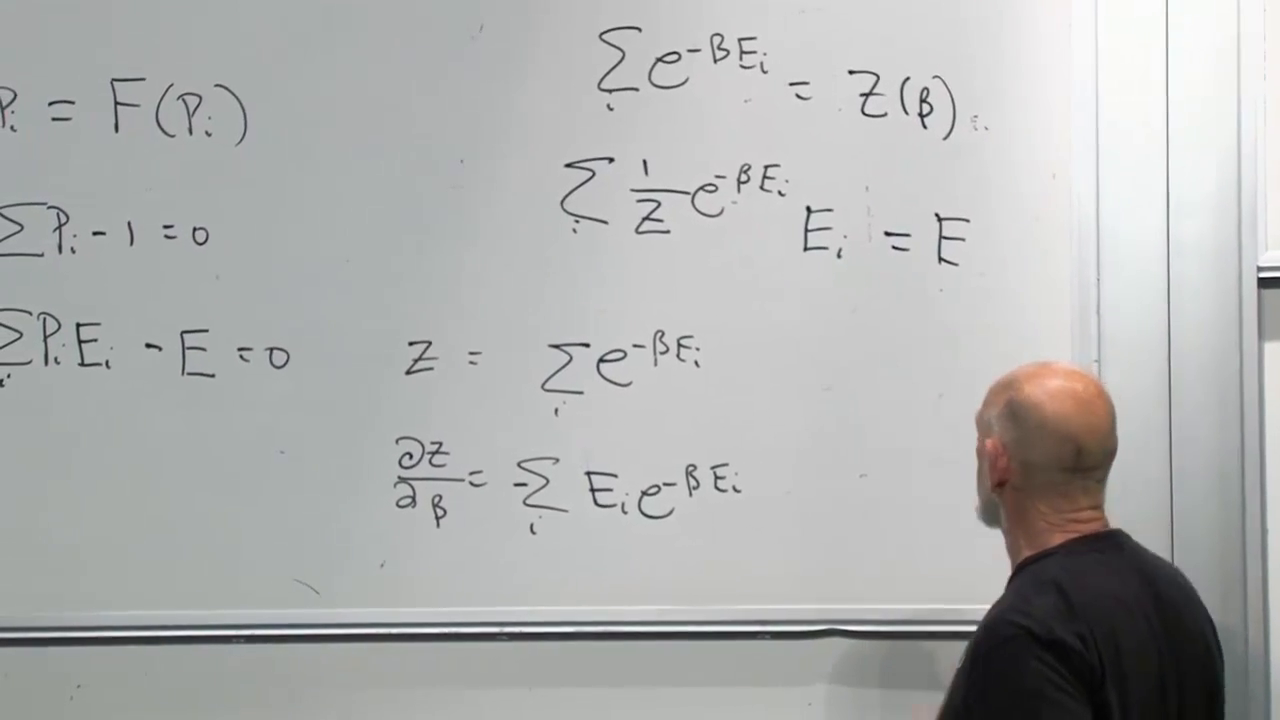
\includegraphics[width=0.82\textwidth]{lecture_04_figure_03.png}
\caption{归一化条件、平均能量约束以及配分函数的导数一同出现在黑板上。}
\lectureframe{00:26:24}
\end{figure}

\begin{classroomqa}
\audiencequestion{黑板下方的方程是关于\(Z\)的新方程，还是由它上方的定义得到的？}
\lecturerresponse{它是对定义
\(Z=\sum_i e^{-\beta E_i}\)求导得到的。求导会带下
\(-E_i\)。再将结果除以\(Z\)，就重现了定义平均能量的那个加权求和。
\lecturetimestamp{00:25:58--00:26:37}}
\end{classroomqa}

\begin{classroomqa}
\audiencequestion{
\(dZ/d\beta=-E Z\)是否使\(Z\)成为微分算子的本征函数？}
\lecturerresponse{并非通常意义上的本征函数。本征值方程应当是一个常数乘以\(Z\)，而这里
\(E=E(\beta)\)。这个方程告诉我们平均能量作为
\(\beta\)的函数；它不是一个固定本征值问题。
\lecturetimestamp{00:28:49--00:29:43}}
\end{classroomqa}

\eqref{eq:sm4-energy-logz}的简洁性具有欺骗性。能谱可能很复杂，计算\(Z\)也可能很困难，但一旦求出这个单一函数，平均能量只需一次求导即可得到。这种模式在统计力学中反复出现：以正确的顺序施加基本运算，就能得到直接猜测会很困难的结果。

\begin{classroomqa}
\audiencequestion{\(E\)是所有复本的总能量，还是每个盒子的平均能量？}
\lecturerresponse{它是一个盒子的平均能量。复本集合的总能量为\(\mathcal N E\)。之后，当系统本身被选为一个包含\(N\)个气体粒子的完整盒子时，\(E\)将表示整个气体样本的能量。
\lecturetimestamp{00:30:55--00:31:10}}
\end{classroomqa}

\begin{classroomqa}
\audiencequestion{我们可以对
\(\sum_i e^{-\beta E_i}\)逐项取对数吗？}
\lecturerresponse{不可以。对数把乘积变成求和，而不是把求和变成对数之和：
\[
 \log\!\left(\sum_i e^{-\beta E_i}\right)
 \ne \sum_i\log\!\left(e^{-\beta E_i}\right).
\]
这一区别在之后会变得有用，那时独立子系统的配分函数会相乘。
\lecturetimestamp{00:31:10--00:31:58}}
\end{classroomqa}

\section{什么固定，什么允许变化？}

同一组公式中存在若干层次的变量，课堂讨论有意将它们区分开来。

\begin{itemize}
 \item 概率\(p_i\)是原始的未知量。
 \item 一旦系统及其控制参数给定，能级\(E_i\)就是固定的。
 \item 乘子\(\alpha\)已被吸收到归一化
 \(Z=e^{1+\alpha}\)中。
 \item 对于给定的平均能量\(E\)，约束条件确定一个数
 \(\beta\)。然而，在一族平衡态中，既可以使用
 \(E=E(\beta)\)，也可以使用\(\beta=\beta(E)\)。
\end{itemize}

\begin{classroomqa}
\audiencequestion{如果乘子是数，为什么\(\beta\)和
\(E\)现在被当作变量处理？}
\lecturerresponse{对于单个约束问题，它们确实是数。但我们可以比较许多具有相同能谱和不同给定平均能量的平衡问题。在这一族中，\(\beta\)随
\(E\)变化。固定\(E\)就确定\(\beta\)；固定\(\beta\)就确定
\(E\)。这是同一关系的两种读法。
\lecturetimestamp{00:31:58--00:33:27}}
\end{classroomqa}

\begin{classroomqa}
\audiencequestion{\(\alpha\)消失了吗？}
\lecturerresponse{消失的只是它的名字。定义
\(e^{-(1+\alpha)}=1/Z\)把它吸收到\(Z\)中。同时保留\(\alpha\)
和\(Z\)会把同一个归一化参数计算两次。
\lecturetimestamp{00:33:29--00:33:49}}
\end{classroomqa}

能量不必是唯一的守恒量。如果总动量、粒子数、角动量或其他量受到约束，它的期望值就会获得自己的乘子。这种扩展改变了系综，但不改变方法。

\begin{classroomqa}
\audiencequestion{只固定平均能量是否对系统作了过多假设？}
\lecturerresponse{它假设在当前问题中不需要以其他守恒量为条件。例如，如果总动量也被固定，那就再加一个约束和另一个拉格朗日乘子。相比之下，体积、形状和外场在这里是控制参数：它们被固定，并决定能级本身。
\lecturetimestamp{00:33:51--00:35:50}}
\end{classroomqa}

\begin{classroomqa}
\audiencequestion{\(\alpha\)是否应作为能量的另一个自变量出现，而\(Z\)是否依赖于能级\(E_i\)？}
\lecturerresponse{\(\alpha\)已经包含在\(Z\)中，因此它不是独立的自变量。配分函数当然既依赖于固定的谱，也依赖于\(\beta\)。改变控制参数会改变\(E_i\)，从而改变\(Z\)；在当前的\(\beta\)导数运算中，谱保持固定。
\lecturetimestamp{00:35:52--00:37:10}}
\end{classroomqa}

\begin{classroomqa}
\audiencequestion{我们是在改变各个能级\(E_i\)，还是在改变平均能量\(E\)？}
\lecturerresponse{各个能级保持固定。平均能量发生变化，是因为概率发生了变化。因此，这一族由\(E\)参数化，或等价地由\(\beta\)参数化，而始终使用同一组能级\(\{E_i\}\)。
\lecturetimestamp{00:37:12--00:39:04}}
\end{classroomqa}

实际上，温度往往比气体的总能量容易测量得多。我们可以插入温度计；称量相对论质量差并援引\(E=mc^2\)虽然正确，却毫无帮助。为了使\(\beta\)具有可操作性，我们现在必须把它与温度的热力学定义联系起来。

\section{温度之前的熵}

从逻辑上说，熵在先。将玻尔兹曼概率代入\eqref{eq:sm4-entropy}：
\begin{equation}
 \log p_i=-\beta E_i-\log Z.
\end{equation}
于是
\begin{align}
 S
 &=-\sum_i p_i\log p_i\\
 &=\beta\sum_i p_iE_i+\log Z\sum_i p_i\\
 &=\beta E+\log Z.
 \label{eq:sm4-entropy-logz}
\end{align}
归一化求和提供了最后的因子一。这也是亥姆霍兹自由能的最初迹象，因为之后在\(k_B=1\)的单位制下，\(F_{\mathrm H}=-T\log Z\)。

\begin{classroomqa}
\audiencequestion{第一项中的因子\(1/Z\)到哪里去了？}
\lecturerresponse{它已经是\(p_i\)的一部分。求和\(\sum_i p_iE_i\)包含完整的归一化概率，并且按定义就是平均能量\(E\)。
\lecturetimestamp{00:43:19--00:43:26}}
\end{classroomqa}

\begin{classroomqa}
\audiencequestion{\(S=\beta E+\log Z\)中是否应该有一个负号？}
\lecturerresponse{不。熵以一个负号开头，而\(\log p_i=-\beta E_i-\log Z\)还包含另外两个负号。它们产生\eqref{eq:sm4-entropy-logz}中显示的两个正项。
\lecturetimestamp{00:45:53--00:46:03}}
\end{classroomqa}

温度在热力学上由
\begin{equation}
 dE=T\,dS,
 \qquad
 \frac{1}{T}=\frac{dS}{dE},
 \label{eq:sm4-temperature-definition}
\end{equation}
定义，其中所有其他控制参数保持固定。直接对\eqref{eq:sm4-entropy-logz}关于\(E\)求导的第一次尝试很快就会变得杂乱，因为\(\beta\)也依赖于\(E\)。取全微分更简洁：
\begin{align}
 dS
 &=\beta\,dE+E\,d\beta
   +\frac{d\log Z}{d\beta}\,d\beta\\
 &=\beta\,dE+E\,d\beta-E\,d\beta\\
 &=\beta\,dE.
 \label{eq:sm4-entropy-differential}
\end{align}
消去利用了\eqref{eq:sm4-energy-logz}。将\eqref{eq:sm4-entropy-differential}与\eqref{eq:sm4-temperature-definition}比较，得到
\begin{equation}
 T=\frac{1}{\beta},
 \qquad
 \beta=\frac{1}{T}.
 \label{eq:sm4-beta-temperature}
\end{equation}

\begin{figure}[t]
\centering
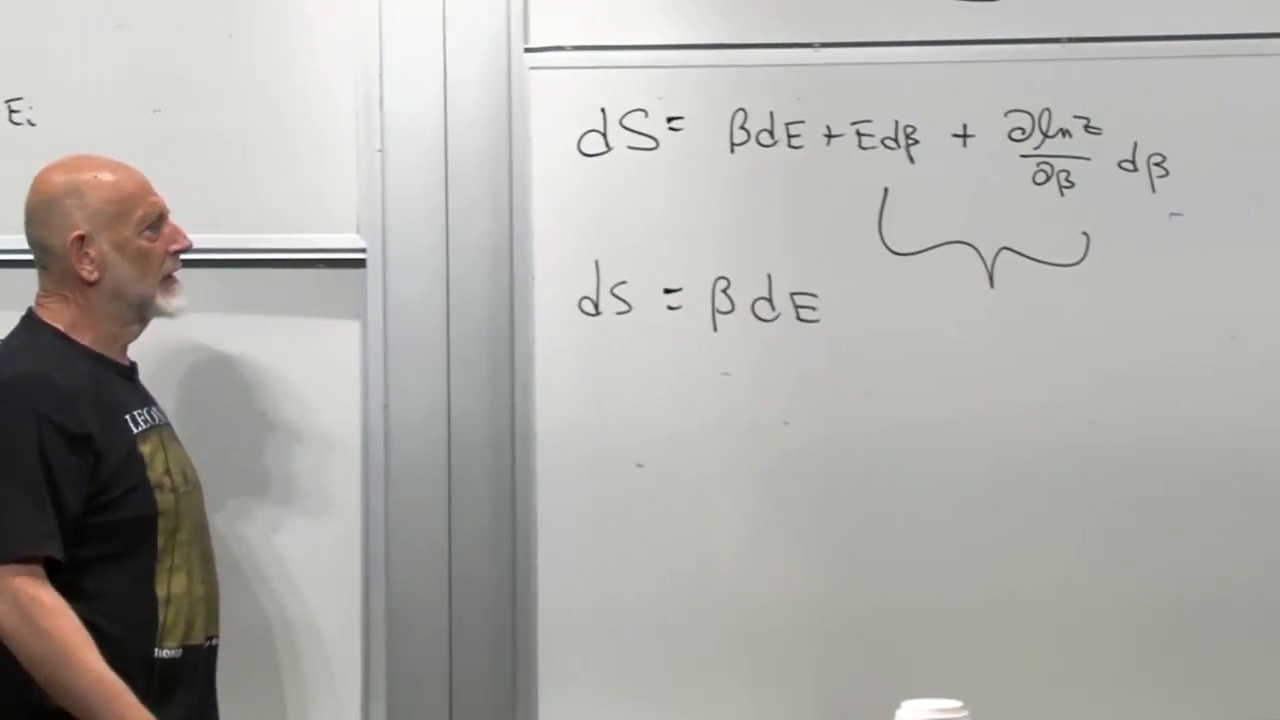
\includegraphics[width=0.82\textwidth]{lecture_04_figure_04.png}
\caption{两个\(d\beta\)项相消，剩下\(dS=\beta\,dE\)。}
\lectureframe{00:50:48}
\end{figure}

\begin{classroomqa}
\audiencequestion{这种相消是否错误地假设了\(\log Z\)与能量或温度无关？}
\lecturerresponse{不。对于固定的谱，只有一个独立的热力学参数。我们可以写出\(Z=Z(\beta)\)，然后沿平衡族将\(\beta=\beta(E)\)视为函数。全微分保留了完整的\(d\beta\)依赖关系，而恒等式\(d\log Z/d\beta=-E\)正是使相消成立的原因。
\lecturetimestamp{00:52:04--00:52:44}}
\end{classroomqa}

在大部分计算中，温度以能量单位计量，因此\(k_B=1\)。恢复实验室单位后，
\begin{equation}
 \beta=\frac{1}{k_B T_{\mathrm K}},
 \label{eq:sm4-beta-laboratory}
\end{equation}
其中\(T_{\mathrm K}\)是以开尔文表示的绝对温度。通常方便地写出\(T_{\mathrm e}=k_BT_{\mathrm K}\)，然后使用\(\beta=1/T_{\mathrm e}\)。

\begin{classroomqa}
\audiencequestion{对于一定体积的气体，系统是一个分子还是整个集合？}
\lecturerresponse{这取决于系统如何定义。这里系统将是整箱气体，因此\(E\)是其所有分子的能量。对于足够稀薄的理想气体，一个分子也可以被视为一个子系统，因为粒子之间不发生相互作用；下面的因子化将展示这两种描述之间的关系。
\lecturetimestamp{00:53:32--00:54:49}}
\end{classroomqa}

现在可以汇总正则系综的各个恒等式：
\begin{align}
 p_i&=\frac{e^{-\beta E_i}}{Z},&
 Z(\beta)&=\sum_i e^{-\beta E_i},\label{eq:sm4-canonical-pair}\\
 E&=-\frac{d\log Z}{d\beta},&
 S&=\beta E+\log Z,&
 T&=\frac{1}{\beta}.
 \label{eq:sm4-canonical-identities}
\end{align}

\section{经典理想气体}

取\(N\)个质量为\(m\)的全同点粒子，置于体积为\(V\)的盒子中。当粒子之间的相互作用可以忽略时，气体是理想的。这可能是一个好的近似，因为力很弱，或者因为气体足够稀薄，近距离相遇很少发生。

一个经典微观态由所有位置和动量指定：
\begin{equation}
 (\bm q_1,\ldots,\bm q_N;\bm p_1,\ldots,\bm p_N).
\end{equation}
有\(3N\)个位置坐标和\(3N\)个动量坐标，因此该状态是\(6N\)维相空间中的一个点。在没有相互作用的情况下，哈密顿量为
\begin{equation}
 H(\bm p)=\sum_{a=1}^{N}\frac{\bm p_a^2}{2m}
 =\sum_{\mu=1}^{3N}\frac{p_\mu^2}{2m}.
 \label{eq:sm4-ideal-hamiltonian}
\end{equation}

\begin{classroomqa}
\audiencequestion{有\(3N\)个粒子吗？对所有动量分量求和是否会重复计算状态？}
\lecturerresponse{有\(N\)个粒子和\(3N\)个动量分量。\eqref{eq:sm4-ideal-hamiltonian}中的求和对每个分量包含一个二次项。相空间积分随后对每个独立分量恰好积分一次，因此该乘积不会导致重复计数。
\lecturetimestamp{01:02:29--01:04:04}}
\end{classroomqa}

对于连续经典相空间，态求和变为
\begin{equation}
 Z_N
 =\frac{1}{N!\,h^{3N}}
 \int_{V^N}d^{3N}q
 \int_{\mathbb R^{3N}}d^{3N}p\,
 e^{-\beta H(\bm p)}.
 \label{eq:sm4-classical-partition}
\end{equation}
讲座聚焦于积分，并写出不带相空间单元\(h^{3N}\)的同一表达式。将其恢复使\(Z_N\)无量纲，并记录了经典态计数的量子起源。由于\(h\)与\(\beta\)无关，它不改变下文所用的能量导数。

位置积分是直接的。哈密顿量与位置无关，每个粒子可以位于盒子中的任何位置：
\begin{equation}
 \int_{V^N}d^{3N}q=V^N.
\end{equation}
动量积分分解为\(3N\)个相同的一维高斯积分：
\begin{equation}
 Z_N
 =\frac{V^N}{N!\,h^{3N}}
 \left[
  \int_{-\infty}^{\infty}dp\,
  e^{-\beta p^2/(2m)}
 \right]^{3N}.
 \label{eq:sm4-factorized-gas}
\end{equation}

因子\(1/N!\)标识了仅因相同粒子的置换而不同的构型。对于固定\(N\)和\(V\)下的平均能量，它只对\(\log Z_N\)贡献一个与\(\beta\)无关的常数，因此在\(-\partial/\partial\beta\)下消失。但它并非在每个问题中都可随意丢弃：与\(h^{3N}\)一起，它对于无量纲配分函数、广延熵和一致化学势是必不可少的。

现在令
\begin{equation}
 x=\sqrt{\frac{\beta}{2m}}\,p,
 \qquad
 dp=\sqrt{\frac{2m}{\beta}}\,dx.
\end{equation}
高斯积分变为
\begin{align}
 \int_{-\infty}^{\infty}dp\,e^{-\beta p^2/(2m)}
 &=
 \sqrt{\frac{2m}{\beta}}
 \int_{-\infty}^{\infty}dx\,e^{-x^2}\\
 &=\sqrt{\frac{2\pi m}{\beta}}.
 \label{eq:sm4-gaussian}
\end{align}

\begin{figure}[t]
\centering
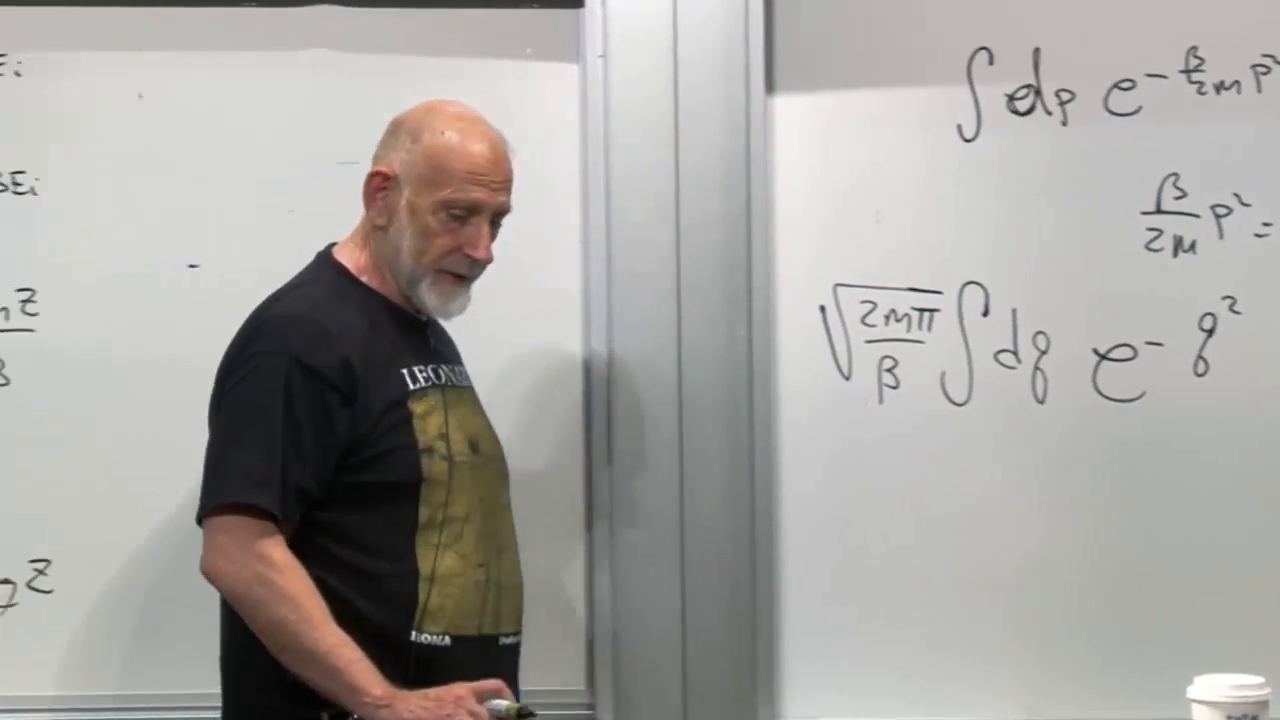
\includegraphics[width=0.82\textwidth]{lecture_04_figure_05.png}
\caption{通过一次重标度，动量积分被化为标准高斯积分。}
\lectureframe{01:13:12}
\end{figure}

代入\eqref{eq:sm4-factorized-gas}得到
\begin{equation}
 Z_N
 =\frac{V^N}{N!\,h^{3N}}
 \left(\frac{2\pi m}{\beta}\right)^{3N/2}.
 \label{eq:sm4-ideal-partition}
\end{equation}

\begin{figure}[t]
\centering
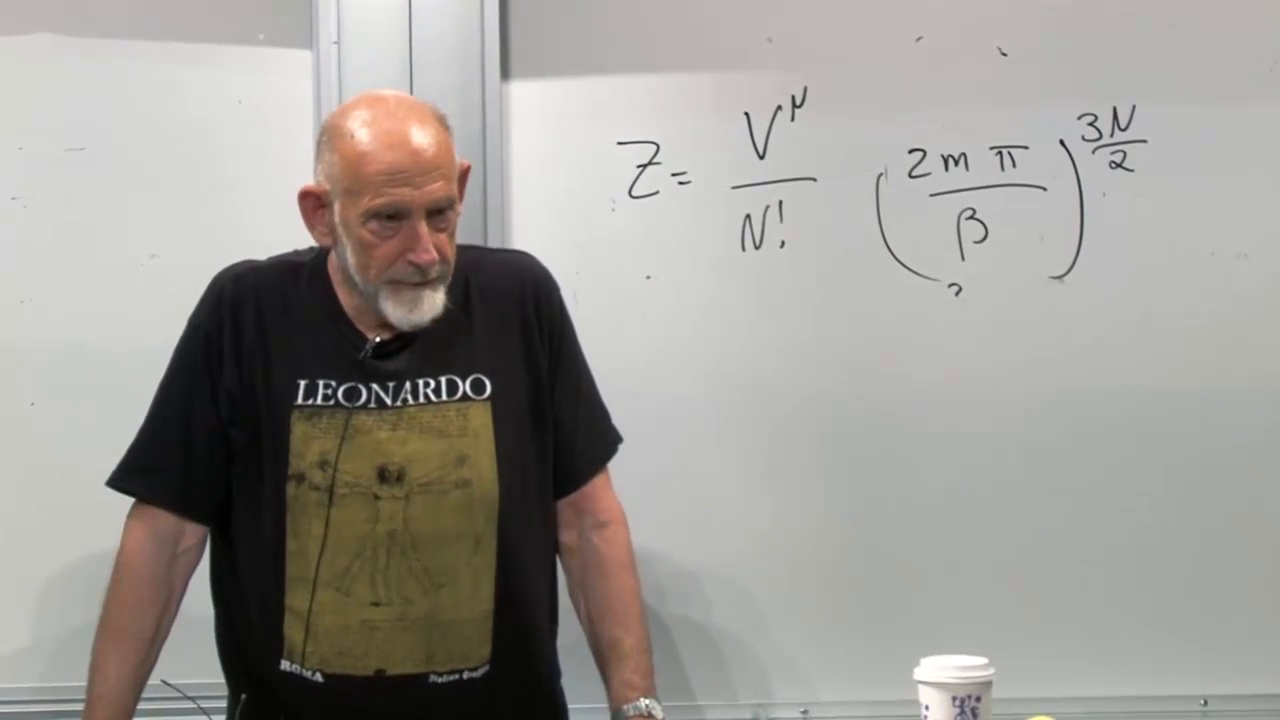
\includegraphics[width=0.78\textwidth]{lecture_04_figure_06.png}
\caption{黑板上完成的理想气体配分函数。相空间单元\(h^{3N}\)在\eqref{eq:sm4-ideal-partition}中被恢复。}
\lectureframe{01:14:38}
\end{figure}

用热德布罗意波长将同一结果打包是有用的
\begin{equation}
 \lambda_T=\frac{h}{\sqrt{2\pi mT}}
 \qquad (k_B=1).
\end{equation}
于是
\begin{equation}
 Z_N=\frac{1}{N!}\left(\frac{V}{\lambda_T^3}\right)^N.
 \label{eq:sm4-thermal-wavelength-form}
\end{equation}

对于宏观的\(N\)，斯特林公式给出
\begin{equation}
 N!\simeq N^Ne^{-N}\sqrt{2\pi N}.
\end{equation}
只保留主导指数依赖并定义\(\rho=N/V\)，
\begin{equation}
 \frac{V^N}{N!}
 \simeq
 \frac{1}{\sqrt{2\pi N}}
 \left(\frac{e}{\rho}\right)^N.
 \label{eq:sm4-density-rewrite}
\end{equation}
这是讲座中简洁的密度重写。平方根因子在\(\log Z_N\)中是次主导的，但这里将其显示出来，而不是悄悄丢弃。

\begin{classroomqa}
\audiencequestion{如果\(1/N!\)与\(\beta\)无关，它是否完全不起作用？}
\lecturerresponse{对于当前固定\(N\)和\(V\)下的平均能量导数，它不起作用，因为它对\(\log Z_N\)添加了一个与\(\beta\)无关的常数。它对于绝对熵和粒子数变化确实有影响。有限的导数陈述与更广泛的态计数陈述不应混淆。
\lecturetimestamp{01:27:01--01:27:51}}
\end{classroomqa}

\section{能量与均分}

乘积难以求导；对数将它们变为求和。由\eqref{eq:sm4-ideal-partition}，
\begin{equation}
 \log Z_N
 =-\frac{3N}{2}\log\beta+\text{\(\beta\)-independent terms}.
 \label{eq:sm4-log-ideal-partition}
\end{equation}
因此
\begin{equation}
 E
 =-\frac{\partial\log Z_N}{\partial\beta}
 =\frac{3N}{2\beta}
 =\frac{3N}{2}T.
 \label{eq:sm4-ideal-energy}
\end{equation}
每个粒子的能量为
\begin{equation}
 \frac{E}{N}=\frac{3}{2}T
 \qquad (k_B=1),
\end{equation}
或者，用实验室单位表示，
\begin{equation}
 \frac{E}{N}=\frac{3}{2}k_BT_{\mathrm K}.
 \label{eq:sm4-ideal-energy-lab}
\end{equation}

\begin{figure}[t]
\centering
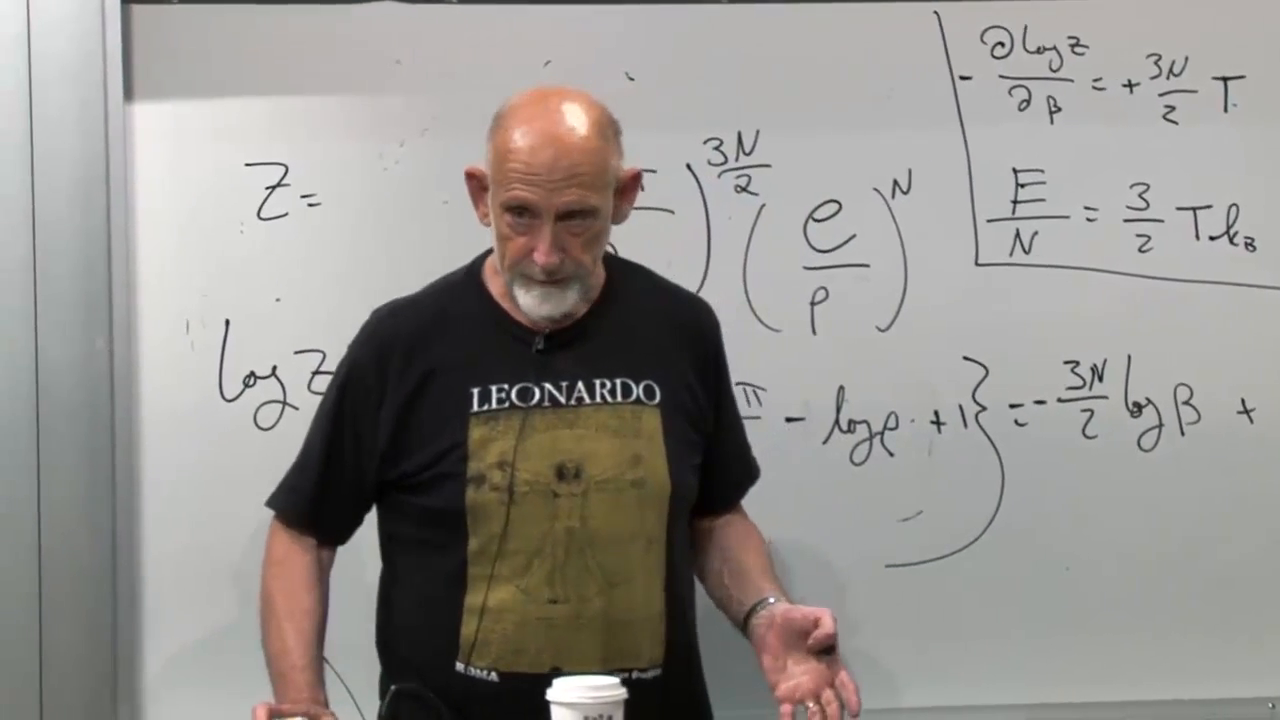
\includegraphics[width=0.84\textwidth]{lecture_04_figure_07.png}
\caption{只有\(-3N\log\beta/2\)项对理想气体能量有贡献，给出\(E/N=3T/2\)。}
\lectureframe{01:25:28}
\end{figure}

\begin{classroomqa}
\audiencequestion{玻尔兹曼常数如何进入能量公式？}
\lecturerresponse{理论家的温度\(T\)是一种能量。要使用开尔文，将其替换为\(k_BT_{\mathrm K}\)，得到\(E/N=3k_BT_{\mathrm K}/2\)。\(k_B\)的小数值将看似宏观的数值温度转换为单个分子的微观能量尺度。
\lecturetimestamp{01:24:58--01:26:01}}
\end{classroomqa}

3来自空间的三个方向。1/2来自每个高斯积分对\(1/\beta\)的平方根依赖。每个独立的二次动量坐标对平均能量贡献
\begin{equation}
 \frac{1}{2}T
\end{equation}
在\(d\)个空间维度中，同样的论证给出\(E/N=dT/2\)。这是均分定理的首次出现。

讲座末尾布置的熵计算由\(S=\beta E+\log Z_N\)得出。使用斯特林近似，
\begin{equation}
 \frac{S}{N}
 \simeq
 \log\!\left[
  \frac{V}{N}
  \left(\frac{2\pi mT}{h^2}\right)^{3/2}
 \right]
 +\frac{5}{2},
 \label{eq:sm4-sackur-tetrode}
\end{equation}
直到次主导的有限\(N\)修正。恢复\(k_B\)将右侧乘以\(k_B\)，并将\(T\)替换为\(k_BT_{\mathrm K}\)。结果清楚地表明，为什么从能量中消失的归一化因子对于熵是不可或缺的。

\section{将气体置于引力场中}

关于把盒子放在中子星上的问题引出了引力推广。在直面中子星之前，先考虑普通房间中的均匀场 \(g\)。取 \(y=0\) 位于底面积为 \(A\)、高度为 \(L\) 的盒子底部。哈密顿量变为
\begin{equation}
 H=\sum_{a=1}^{N}
 \left(\frac{\bm p_a^2}{2m}+mgy_a\right).
 \label{eq:sm4-gravity-hamiltonian}
\end{equation}
水平方向的坐标积分仍然给出 \(A^N\)，而每个竖直坐标贡献
\begin{equation}
 I_y(L)
 =\int_0^Ldy\,e^{-\beta mgy}
 =\frac{1-e^{-\beta mgL}}{\beta mg}.
 \label{eq:sm4-finite-height-integral}
\end{equation}

\begin{classroomqa}
\audiencequestion{竖直方向的积分真的应该积到无穷远，还是只积到盒子的顶部？}
\lecturerresponse{对于有限高的盒子，它必须从 \(0\) 积到盒子的高度 \(L\)，如 \eqref{eq:sm4-finite-height-integral} 所示。把上限取为无穷远是后来的简化，它模拟的是表面上方的大气，而不是有限的房间。
\lecturetimestamp{01:30:25--01:31:32}}
\end{classroomqa}

因此，完整的有限高度配分函数为
\begin{equation}
 Z_N(L)
 =
 \frac{1}{N!\,h^{3N}}
 \left[
  A\,
  \frac{1-e^{-\beta mgL}}{\beta mg}
  \left(\frac{2\pi m}{\beta}\right)^{3/2}
 \right]^N.
 \label{eq:sm4-gravity-partition-finite}
\end{equation}
竖直方向的因子依赖于 \(\beta\)，所以它必定对能量有贡献。确实，
\begin{equation}
 \langle U\rangle
 =N\left[
  \frac{1}{\beta}
  -\frac{mgL}{e^{\beta mgL}-1}
 \right].
 \label{eq:sm4-finite-gravity-energy}
\end{equation}
这就补完了讲座最初留作繁琐计算的那一小段积分。

对于无限高的大气，\(L\to\infty\)，并且
\begin{equation}
 I_y(\infty)=\frac{1}{\beta mg}.
\end{equation}
配分函数变为
\begin{equation}
 Z_N^{(\infty)}
 =
 \frac{1}{N!\,h^{3N}}
 \left[
  \frac{A}{\beta mg}
  \left(\frac{2\pi m}{\beta}\right)^{3/2}
 \right]^N.
 \label{eq:sm4-gravity-partition-infinite}
\end{equation}
其依赖于 \(\beta\) 的对数为
\begin{equation}
 \log Z_N^{(\infty)}
 =-\frac{3N}{2}\log\beta-N\log\beta+\mathrm{const}.
\end{equation}
第一项给出动能 \(3NT/2\)；第二项给出平均引力势能 \(NT\)。因此，对于这个理想化的无界大气，
\begin{equation}
 E_{\mathrm{tot}}=\frac{5N}{2}T
\end{equation}

\begin{figure}[t]
\centering
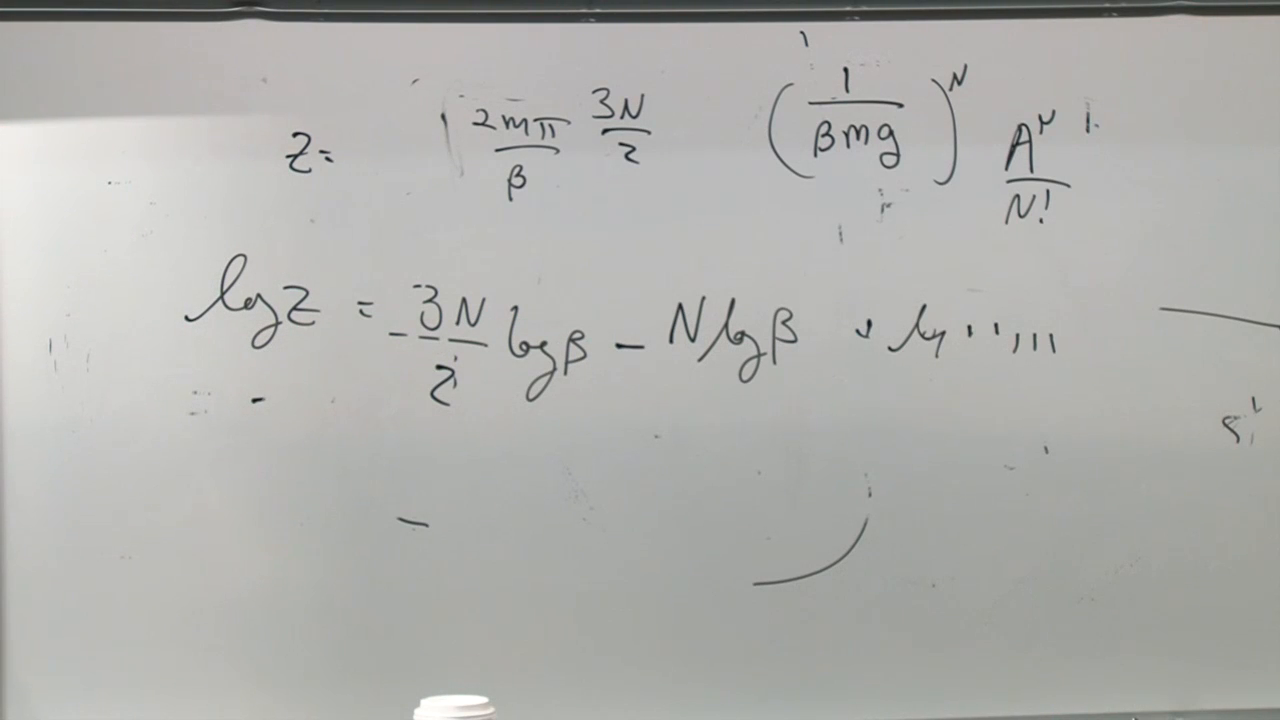
\includegraphics[width=0.83\textwidth]{lecture_04_figure_08.png}
\caption{无限大气配分函数把 \(-N\log\beta\) 加到 \(\log Z\) 上，这就是平均势能的来源。}
\lectureframe{01:36:38}
\end{figure}

\begin{classroomqa}
\audiencequestion{非常强的引力场是否需要另一个拉格朗日乘子？}
\lecturerresponse{并不仅仅因为场强就需要。引力改变哈密顿量，从而改变能级或相空间权重。同一个能量乘子 \(\beta\) 仍然保留。中子星会带来额外的物理复杂性，但第一步修改仍然是把引力势能放入 \(H\)。
\lecturetimestamp{01:27:58--01:29:24}}
\end{classroomqa}

\section{结尾的三个问题}

\begin{classroomqa}
\audiencequestion{哪一个方程是玻尔兹曼分布，它关于平衡断言了什么？}
\lecturerresponse{该分布为
\[
 p_i=\frac{e^{-\beta E_i}}{Z}.
\]
它是在归一化和固定平均能量的约束下具有最大熵的分布。平均能量必须由同一组概率计算，而归一化仍然必须被强制满足，尽管它在最终公式中看起来几乎是自动成立的。
\lecturetimestamp{01:38:14--01:38:45}}
\end{classroomqa}

这套程序可能显得机械：写出配分函数，取对数，然后求导。然而由此得到的方程仍然不断令人惊讶。熟悉会让人知道哪种简单操作应当接在哪种操作之后，但这并不会使这门学科变得不那么奇妙。

\begin{classroomqa}
\audiencequestion{这些熵的思想能应用于坍缩的恒星或黑洞吗？当物质占据更小的区域时，熵怎么能增加？}
\lecturerresponse{恒星之所以困难，主要是因为其物质细节很复杂。黑洞有一个更干净的基准：在给定的宏观约束下，它的贝肯斯坦--霍金熵是极限引力熵。坍缩可以使熵增加，直到达到那个黑洞值；要进一步增加它，就需要改变可用的能量或尺度。
\lecturetimestamp{01:39:29--01:40:36}}
\end{classroomqa}

\begin{classroomqa}
\audiencequestion{配分函数也能计算能量的涨落吗？}
\lecturerresponse{能。一阶导数给出平均能量，二阶导数给出其方差：
\begin{align*}
 \frac{\partial^2\log Z}{\partial\beta^2}
 &=\langle E^2\rangle-\langle E\rangle^2\\
 &=\operatorname{Var}(E).
\end{align*}
以能量单位表示，它与热容的关系为 \(\operatorname{Var}(E)=T^2C_V\)。以实验室单位表示，
\(\operatorname{Var}(E)=k_BT_{\mathrm K}^2C_V\)。这个涨落关系就是下一次计算。
\lecturetimestamp{01:40:37--01:41:53}}
\end{classroomqa}

涨落把统计力学与纯粹连续的热力学描述区分开来。对它们的系统研究尤其与吉布斯和爱因斯坦相关，它揭示了光滑宏观定律背后的有限微观组分。下一讲就从这里开始。
\chapter{压强、自由能与能量涨落}

\lectureoverview{我们不假设分子撞击器壁的动理学图像，而是从配分函数导出压强。一个几何引理把绝热导数化为固定温度下的导数，亥姆霍兹自由能提供了通向\(\log Z\)的桥梁，理想气体定律则作为第一个应用随之得出。随后我们用同一个配分函数导出平衡能量涨落及其与热容的关系。}

\section{让数学来检验直觉}

热力学有着一种奇特的名声。它的微积分是初等的，然而选择对什么求导、把什么固定住却可能极为微妙。我们的问题是有意收窄的：计算理想气体的压强。然而，通往这一答案的路径被设计得足够普遍，以便适用于那些熟悉的分子图像不再可靠的情形。

动理学的说法很容易讲。分子撞击器壁，并使其动量的法向分量反向。单位时间内传递的动量给出力，而单位面积上的力给出压强。我们已经知道，三维中每个分子的平均动能为
\begin{equation}
 \left\langle \frac{p^2}{2m}\right\rangle=\frac{3}{2}T
 \qquad (k_B=1).
 \label{eq:sm5-mean-kinetic-energy}
\end{equation}
在速度分布各向同性的情况下，人们可以估计碰撞率、每次碰撞中的动量转移以及由此产生的压强。

但器壁本身似乎破坏了各向同性。为什么紧邻边界的分子应当与内部深处的分子具有相同的速率和方向分布？在平衡态下，就此处相关的精度而言，它们确实如此，但这一结论应当从统计力学得出，而不是作为直觉偷偷塞进计算之中。分子之间的碰撞使动理论论证更加不透明。无相互作用气体之所以容易，恰恰因为它是一个异常简单的系统。

物理学中有些时候，最稳妥的做法是暂时压制图像，让数学来驾驭。人们先确定待求的量，操纵一般关系，然后等待一个可辨认的公式出现。直觉在最后回归，但那时是数学在检验直觉，而不是反过来。热力学的乐趣就在于这一过程中涌现出的令人惊讶的关系。

所需的关系是一个状态方程，
\begin{equation}
 P=P(T,V,N),
 \label{eq:sm5-equation-of-state-target}
\end{equation}
其中\(N\)是物质的量，\(T\)是温度，\(V\)是体积。一个令人满意的推导应当在粒子相互作用时，或者当物质是液体、等离子体或固体时，仍然说得通。只有配分函数的最终求值才会专门化到理想气体。

\section{熵与亥姆霍兹自由能}

首先取回后面将要用到的正则公式。对于以\(i\)标记的微观态，
\begin{equation}
 \begin{aligned}
 S&=-\sum_i p_i\log p_i,\\
 p_i&=\frac{e^{-\beta E_i}}{Z},\\
 Z&=\sum_i e^{-\beta E_i}.
 \end{aligned}
 \label{eq:sm5-canonical-definitions}
\end{equation}
概率的对数为
\begin{equation}
 \log p_i=-\beta E_i-\log Z.
 \label{eq:sm5-log-probability}
\end{equation}
代入熵的表达式得到
\begin{align}
 S
 &=-\sum_i p_i\log p_i \notag\\
 &=\beta\sum_i p_iE_i+\log Z\sum_i p_i \notag\\
 &=\beta E+\log Z.
 \label{eq:sm5-entropy-log-z}
\end{align}
这里\(E=\sum_i p_iE_i\)是平均能量。

\begin{classroomqa}
\audiencequestion{为什么第二项只给出\(\log Z\)，而不是态数乘以\(\log Z\)？}
\lecturerresponse{被求和的系数是\(p_i\)，而不是\(1\)。归一化给出\(\sum_i p_i=1\)。等价地，分子\(\sum_i e^{-\beta E_i}=Z\)与分母中的\(Z\)相消。态数在这一步中从未出现。
\lecturetimestamp{00:14:25--00:14:55}}
\end{classroomqa}

在本讲大部分内容所用的能量单位下，
\(\beta=1/T\)。将\eqref{eq:sm5-entropy-log-z}乘以\(T\)并重新整理，得到
\begin{equation}
 E-TS=-T\log Z.
 \label{eq:sm5-helmholtz-identity}
\end{equation}
左边的组合出现得如此频繁，值得给它一个名字：
\begin{equation}
 A\equiv E-TS,
 \qquad
 A=-T\log Z.
 \label{eq:sm5-helmholtz-definition}
\end{equation}
它就是亥姆霍兹自由能。此刻这个名字不如这个恒等式本身重要；当把压强转化为配分函数的导数时，我们将需要这个恒等式。

\begin{figure}[t]
\centering
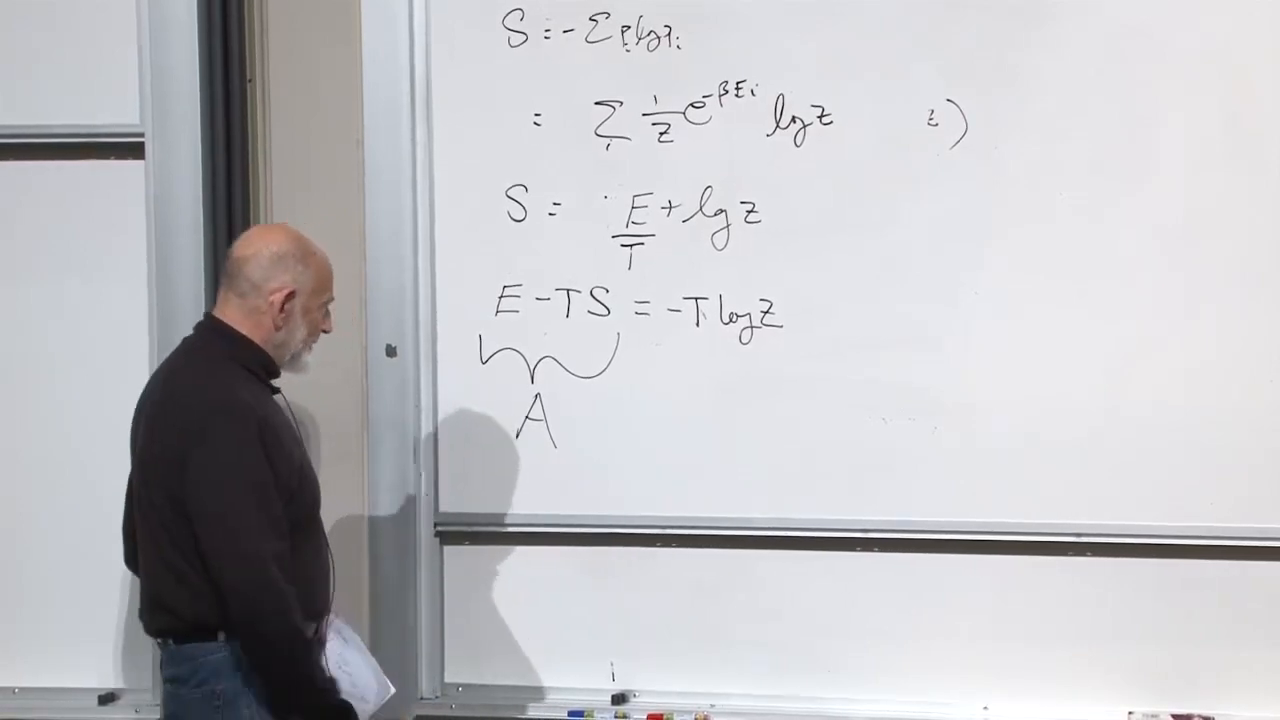
\includegraphics[width=0.90\textwidth]{lecture_05_figure_03.png}
\caption{正则熵关系被重新整理为
\(A=E-TS=-T\log Z\)。}
\lectureframe{00:16:50}
\end{figure}

\section{控制参量及其响应}

控制参量是实验者可以从外部改变的宏观量。移动活塞改变体积，而无需操纵单个分子。外加电场和磁场是另外的例子。在更一般的系综中，粒子数也可以被允许改变。

热力学变量自然地成共轭对出现。体积是当前问题中的控制参量，压强是它的响应。我们改变\(V\)；压强告诉我们系统在能量上如何抵抗这一改变。稍后，能量的导数将使这种配对变得精确。

\begin{classroomqa}
\audiencequestion{压力本身能否被视为控制参量？}
\lecturerresponse{人们可以设计一个固定外部压力的实验，但在本文所用的构造中，活塞位置固定体积，而内部压力是响应量。压力与体积是共轭变量；其中哪一个被控制取决于系综和装置。
\lecturetimestamp{00:19:22--00:20:01}}
\end{classroomqa}

\begin{classroomqa}
\audiencequestion{是否假定所有分子都相同，还是该论证仅限于气体？}
\lecturerresponse{热力学论证不需要这样的限制。圆筒中可以含有多种组分、液体，甚至正在被压缩的固体。只有在一般压力公式建立之后，理想气体配分函数才会成为一个特殊应用。
\lecturetimestamp{00:20:02--00:20:39}}
\end{classroomqa}

\begin{classroomqa}
\audiencequestion{物质的量能否作为另一种外部操作而改变？}
\lecturerresponse{可以。粒子数也是一种可能的控制参量。对它作动力学处理会引出其自身的共轭变量，即化学势。对于今晚的计算，\(N\)保持固定。
\lecturetimestamp{00:20:39--00:20:57}}
\end{classroomqa}

\begin{classroomqa}
\audiencequestion{液态水和蒸汽能否同时处于平衡？}
\lecturerresponse{在共存温度和压力下，它们可以。重力可能使液体位于蒸气下方，但两相仍可共享同一温度并保持热平衡。同一套一般统计力学框架仍然适用。
\lecturetimestamp{00:20:59--00:21:36}}
\end{classroomqa}

对于接下来的论证，把能量和熵视为两个可独立调节变量的依赖函数：
\begin{equation}
 E=E(T,V),
 \qquad
 S=S(T,V).
 \label{eq:sm5-dependent-functions}
\end{equation}
温度和体积给出热力学状态空间上的坐标。能量和熵为该空间中的每一个平衡点赋予数值。

\section{定熵导数}

我们最终需要的导数并不寻常：
\[
 \left(\frac{\partial E}{\partial V}\right)_S.
\]
尽管\(T\)和\(V\)是独立坐标，这个导数要求我们在约束依赖函数\(S(T,V)\)保持恒定的同时改变\(V\)。它是沿\((T,V)\)平面中一条曲线的导数，而不是沿坐标轴的导数。

\begin{classroomqa}
\audiencequestion{如果后面要用到导数\(dT/dV\)，那么\(T\)和\(V\)怎么还能是独立的？}
\lecturerresponse{在整个状态空间上，它们是独立的。一旦施加约束\(S(T,V)=\mathrm{constant}\)，允许的状态就位于一条一维等值线上。沿该等值线，\(T\)成为\(V\)的函数，其斜率\(dT/dV\)有良好定义。
\lecturetimestamp{01:01:18--01:02:09}}
\end{classroomqa}

\begin{lemma}
若\(E(T,V)\)和\(S(T,V)\)可微，则在\((\partial S/\partial T)_V\neq0\)处，
\begin{equation}
 \left(\frac{\partial E}{\partial V}\right)_S
 =
 \left(\frac{\partial E}{\partial V}\right)_T
 -
 \left(\frac{\partial E}{\partial S}\right)_V
 \left(\frac{\partial S}{\partial V}\right)_T.
 \label{eq:sm5-calculus-lemma}
\end{equation}
\end{lemma}

\begin{proof}
对于任意无穷小位移，
\begin{equation}
 dE=
 \left(\frac{\partial E}{\partial V}\right)_T dV
 +
 \left(\frac{\partial E}{\partial T}\right)_V dT.
 \label{eq:sm5-total-differential-e}
\end{equation}
在固定\(V\)时，链式法则允许把\(S\)用作中间变量：
\begin{equation}
 \left(\frac{\partial E}{\partial T}\right)_V
 =
 \left(\frac{\partial E}{\partial S}\right)_V
 \left(\frac{\partial S}{\partial T}\right)_V.
 \label{eq:sm5-chain-rule-e-s-t}
\end{equation}

现在把位移限制在\(S\)为常数的等值线上。沿该等值线，
\begin{equation}
 0=dS=
 \left(\frac{\partial S}{\partial V}\right)_T dV
 +
 \left(\frac{\partial S}{\partial T}\right)_V dT.
 \label{eq:sm5-constant-entropy-differential}
\end{equation}
解出等值线斜率，得到
\begin{equation}
 \left(\frac{dT}{dV}\right)_S
 =
 -
 \frac{\left(\frac{\partial S}{\partial V}\right)_T}
 {\left(\frac{\partial S}{\partial T}\right)_V}.
 \label{eq:sm5-entropy-contour-slope}
\end{equation}
用\(dV\)除\eqref{eq:sm5-total-differential-e}，使用
\eqref{eq:sm5-chain-rule-e-s-t}，并代入
\eqref{eq:sm5-entropy-contour-slope}：
\begin{align}
 \left(\frac{\partial E}{\partial V}\right)_S
 &=
 \left(\frac{\partial E}{\partial V}\right)_T
 +
 \left(\frac{\partial E}{\partial S}\right)_V
 \left(\frac{\partial S}{\partial T}\right)_V
 \left(\frac{dT}{dV}\right)_S \notag\\
 &=
 \left(\frac{\partial E}{\partial V}\right)_T
 -
 \left(\frac{\partial E}{\partial S}\right)_V
 \left(\frac{\partial S}{\partial V}\right)_T.
\end{align}
因子\((\partial S/\partial T)_V\)已经消去，从而证明了该结果。
\end{proof}

\begin{figure}[t]
\centering
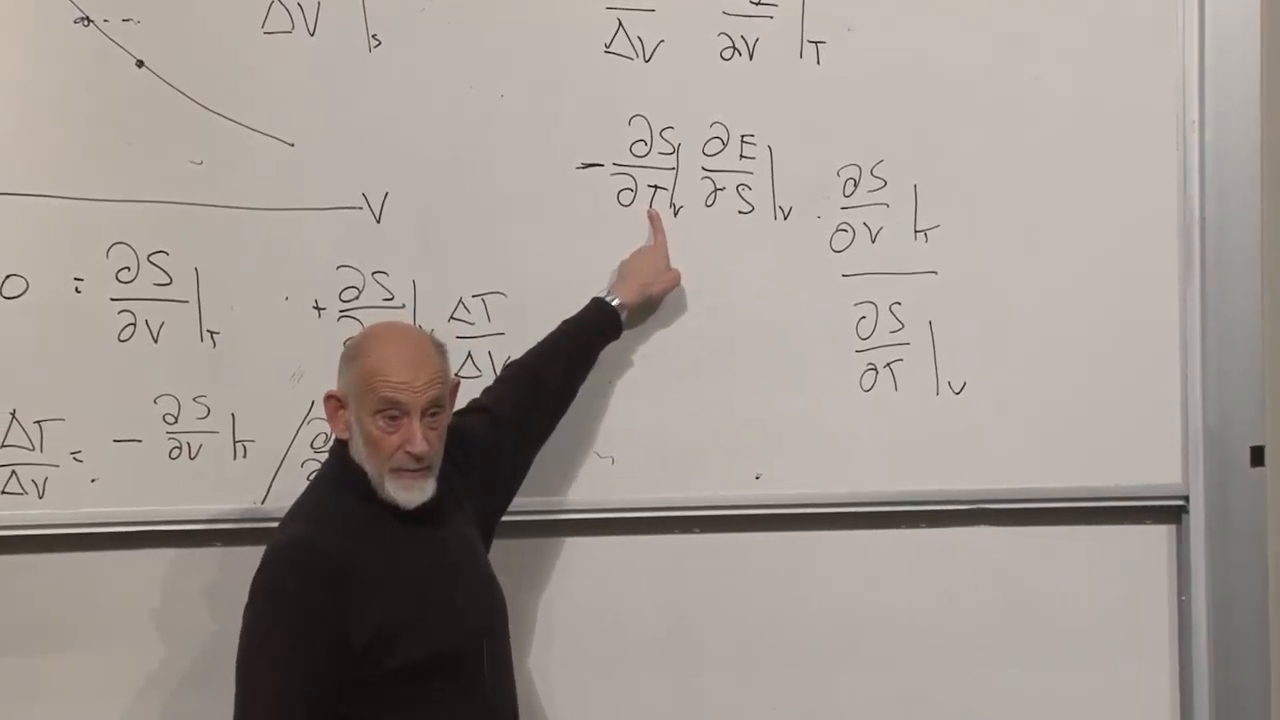
\includegraphics[width=0.90\textwidth]{lecture_05_figure_04.png}
\caption{完成导数引理的定熵等值线计算中的消去。}
\lectureframe{00:36:10}
\end{figure}

几何图像并非装饰。它解释了为什么一个看似奇怪的固定\(S\)导数可以用独立坐标\(T\)和\(V\)下的普通偏导数来求值。在构造过程中写出\(\delta E/\delta V\)，有助于提醒我们这些符号表示沿指定路径的小变化之比。

\begin{classroomqa}
\audiencequestion{\(dE\)的展开是否只是偏导数的普通定义？}
\lecturerresponse{是的。全微分中没有任何特殊之处。唯一额外的要素是随后限制到等值线\(dS=0\)，这决定了\(dT\)与\(dV\)之间的关系。
\lecturetimestamp{00:29:26--00:29:32}}
\end{classroomqa}

\begin{classroomqa}
\audiencequestion{消去是否要求\((\partial S/\partial T)_V\)非零？}
\lecturerresponse{是的。对于普通稳定系统，
\[
 \left(\frac{\partial S}{\partial T}\right)_V
 =\frac{C_V}{T}>0,
\]
所以该除法是合法的。例外点需要另行处理。在哈密顿量固定时，升高温度会加宽正则能量分布，通常增大熵；降低温度则使其变窄。这就是单调性论证在物理上正确的方向。
\lecturetimestamp{00:36:50--00:37:47}}
\end{classroomqa}

\section{活塞功与绝热条件}

现在我们来赋予这个导数物理意义。考虑一个横截面积为\(\mathcal A\)的活塞。如果它向外移动\(dx\)，那么
\begin{equation}
 dV=\mathcal A\,dx.
 \label{eq:sm5-piston-volume}
\end{equation}
气体对活塞施加力\(P\mathcal A\)，因此气体所做的功为
\begin{equation}
 \delta W_{\mathrm{by}}=P\mathcal A\,dx=P\,dV.
 \label{eq:sm5-piston-work}
\end{equation}
如果没有热量进入气体，能量守恒给出
\begin{equation}
 dE=-P\,dV.
 \label{eq:sm5-adiabatic-work}
\end{equation}
符号具有物理意义：在膨胀过程中，气体提升或加速活塞，而自身的能量减少。

\begin{figure}[t]
\centering
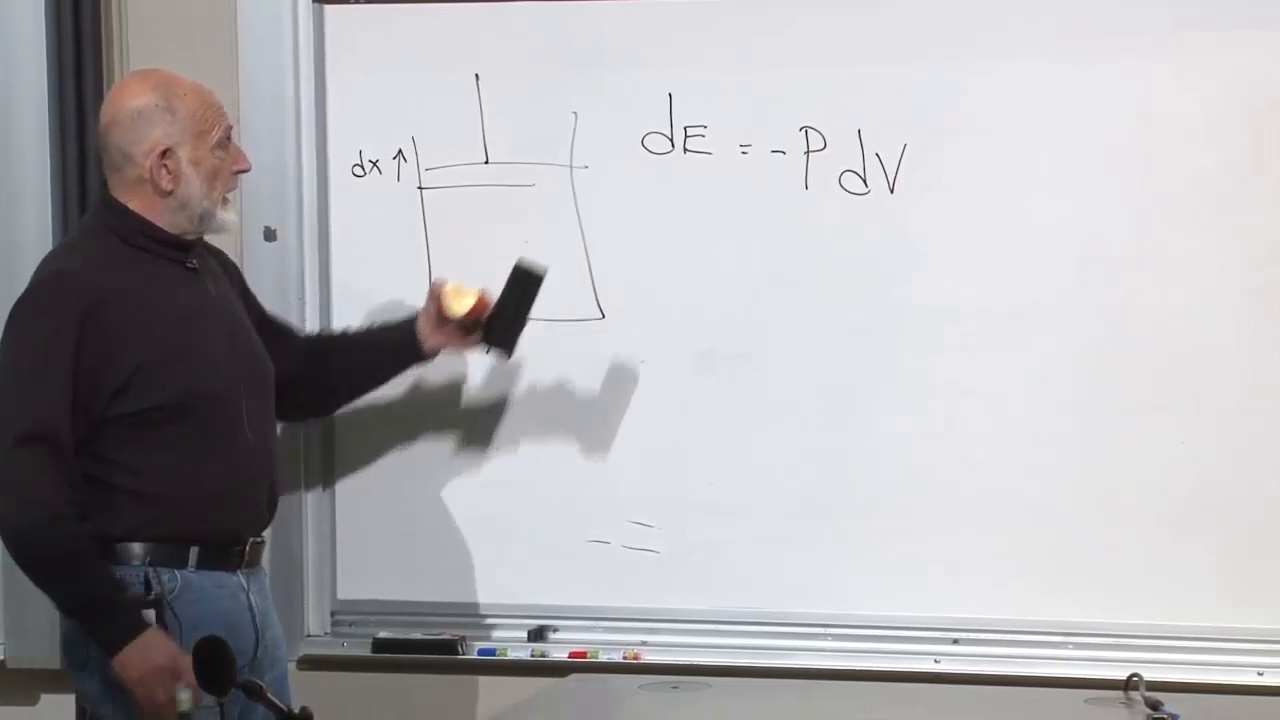
\includegraphics[width=0.90\textwidth]{lecture_05_figure_05.png}
\caption{活塞几何与已完成的功关系\(dE=-P\,dV\)。}
\lectureframe{00:43:10}
\end{figure}

两个限定条件至关重要。活塞必须移动得足够慢，使系统始终任意接近平衡态，并且器壁必须绝热，使能量不以热的形式供给。快速拉动可能快到在运动过程中没有任何分子能够追上后退的活塞。快速压缩会激发冲击波。这两种过程都不能用一系列平衡态来表示。

\emph{绝热}一词有时用于表示无热传递，有时用于表示缓慢变化。在此处所需的可逆过程中，两种含义都涉及：变化是准静态的且热绝缘的。在这些条件下，它也是等熵的。

\begin{classroomqa}
\audiencequestion{为什么绝热变化保持熵不变？}
\lecturerresponse{从量子力学角度考察系统。其多体能级依赖于体积。当\(V\)缓慢变化时，绝热定理将每个被占据的能级连续地变为其后继能级，而不发生能级标号之间的跃迁。能量\(E_i(V)\)发生移动，但占据概率\(p_i\)保持不变。由于
\(S=-\sum_i p_i\log p_i\)依赖于这些概率，熵保持不变。热交换或不可逆运动会使这一结论失效。
\lecturetimestamp{00:43:37--00:49:15}}
\end{classroomqa}

\begin{figure}[t]
\centering
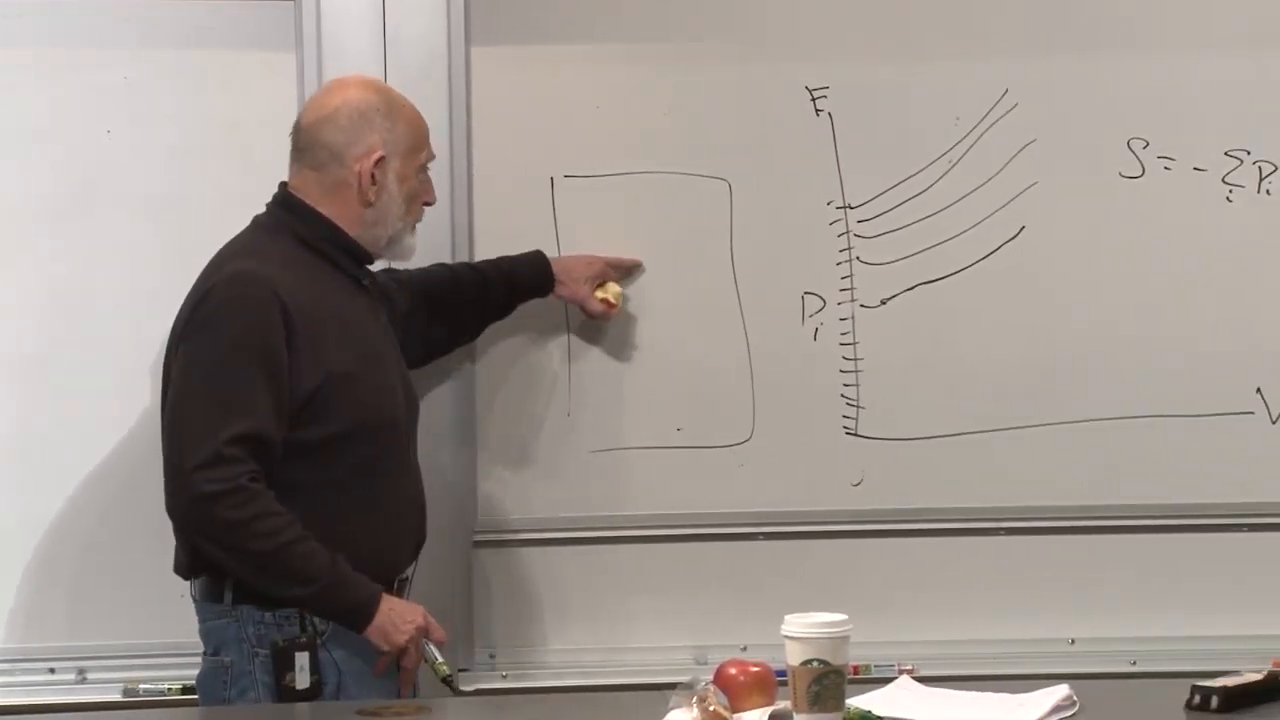
\includegraphics[width=0.90\textwidth]{lecture_05_figure_06.png}
\caption{多体能级随体积移动，而其占据概率保持其能级标号。}
\lectureframe{00:48:50}
\end{figure}

方程\eqref{eq:sm5-adiabatic-work}沿这条等熵路径求值，将压强确定为
\begin{equation}
 P=-\left(\frac{\partial E}{\partial V}\right)_S.
 \label{eq:sm5-pressure-fixed-entropy}
\end{equation}
这就是压强与体积之间的共轭关系。

\begin{classroomqa}
\audiencequestion{如果改为快速移动活塞会发生什么？}
\lecturerresponse{系统离开平衡态，其详细动力学变得重要。突然压缩会产生冲击波。在理想的自由膨胀中，活塞可以在任何分子撞击它之前后退，因此不做功，即使体积发生变化，能量也保持不变。气体随后弛豫到具有增加熵的平衡态。这类过程不能用
\eqref{eq:sm5-pressure-fixed-entropy}中的单一平衡导数来描述。
\lecturetimestamp{00:58:30--01:01:15}}
\end{classroomqa}

\begin{classroomqa}
\audiencequestion{什么定量条件决定一个变化是否缓慢？}
\lecturerresponse{外部变化时间必须远长于相关的内部弛豫时间。对于气体，在宏观变化期间应发生许多分子碰撞和许多器壁撞击。精确的时间尺度取决于材料和几何形状，而准静态极限本身是普遍的。
\lecturetimestamp{01:02:09--01:03:20}}
\end{classroomqa}

\section{从绝热能量到配分函数}

物理公式\eqref{eq:sm5-pressure-fixed-entropy}还不是容易计算的形式。正则系综统计力学自然地给出温度的函数，因为\(T\)直接出现在玻尔兹曼权重中。微积分引理将难以处理的固定熵导数转化为那种计算语言：
\begin{align}
 P
 &=
 -\left(\frac{\partial E}{\partial V}\right)_T
 +
 \left(\frac{\partial E}{\partial S}\right)_V
 \left(\frac{\partial S}{\partial V}\right)_T.
 \label{eq:sm5-pressure-lemma-substitution}
\end{align}
在固定体积下，第一定律给出\(dE=T\,dS\)，因此
\begin{equation}
 \left(\frac{\partial E}{\partial S}\right)_V=T.
 \label{eq:sm5-e-s-temperature}
\end{equation}
于是
\begin{equation}
 P=
 -\left(\frac{\partial E}{\partial V}\right)_T
 +
 T\left(\frac{\partial S}{\partial V}\right)_T.
 \label{eq:sm5-pressure-fixed-temperature-pieces}
\end{equation}

\begin{classroomqa}
\audiencequestion{压强公式中的负号从何而来？}
\lecturerresponse{它起源于气体所做的功：
\(dE=-P\,dV\)在绝热膨胀过程中。微积分引理本身在其两项之间有一个负号；
\(P=-(\partial E/\partial V)_S\)中的整体负号将两者都反转，产生
\eqref{eq:sm5-pressure-fixed-temperature-pieces}。
\lecturetimestamp{00:52:40--00:53:14}}
\end{classroomqa}

由于\(T\)在两个导数中都保持固定，
\begin{align}
 P
 &=
 -\left(\frac{\partial}{\partial V}(E-TS)\right)_T \notag\\
 &=
 -\left(\frac{\partial A}{\partial V}\right)_T.
 \label{eq:sm5-pressure-free-energy}
\end{align}
最后代入\(A=-T\log Z\)：
\begin{equation}
 \boxed{
 P=
 T\left(\frac{\partial\log Z}{\partial V}\right)_T
 }.
 \label{eq:sm5-pressure-log-z}
\end{equation}

\begin{figure}[t]
\centering
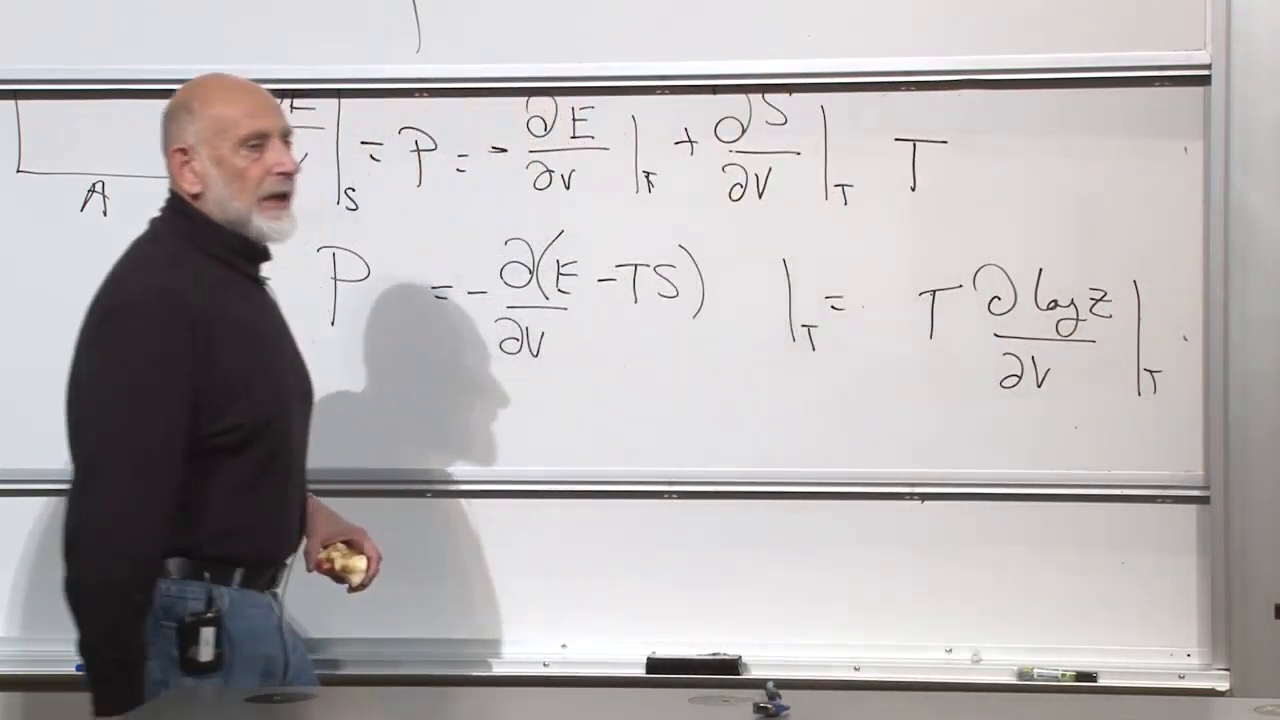
\includegraphics[width=0.90\textwidth]{lecture_05_figure_07.png}
\caption{对宗量的固定温度压缩：
\(P=-(\partial A/\partial V)_T
=T(\partial\log Z/\partial V)_T\)。}
\lectureframe{00:55:55}
\end{figure}

\eqref{eq:sm5-pressure-log-z}中没有任何内容假设理想气体。如果能够为相互作用的流体、等离子体或固体计算出配分函数，同一个导数就给出其压强。更一般地，每个外部控制参数都有一个共轭响应，通过对适当的热力学势求导得到。配分函数将许多这样的响应打包在一起：对\(\log Z\)关于\(\beta\)求导给出能量，而对其关于体积求导给出压强。

\section{理想气体状态方程}

现在才专门考虑\(N\)个无相互作用粒子。保留经典相空间归一化，
\begin{equation}
 Z_N=
 \frac{1}{N!h^{3N}}
 \int d^{3N}q\,d^{3N}p\,
 \exp\!\left[
 -\beta\sum_{a=1}^{N}\frac{\mathbf p_a^2}{2m}
 \right].
 \label{eq:sm5-ideal-gas-partition-integral}
\end{equation}
这里有\(3N\)个位置坐标和\(3N\)个动量坐标。哈密顿量不依赖于位置，因此每个粒子贡献一个容器体积因子：
\begin{equation}
 Z_N=
 \frac{V^N}{N!h^{3N}}I_p(\beta),
 \label{eq:sm5-ideal-gas-factorization}
\end{equation}
其中整个动量积分\(I_p(\beta)\)与\(V\)无关。

\begin{classroomqa}
\audiencequestion{为什么有\(3N\)个位置积分和\(3N\)个动量积分？}
\lecturerresponse{\(N\)个粒子中的每一个都有三个空间坐标和三个共轭动量分量。相空间每一半中的计数都是\(3N\)，而不是\(N\)个粒子加上另外\(3N\)个粒子。
\lecturetimestamp{01:04:19--01:04:28}}
\end{classroomqa}

取对数将体积依赖性分离出来：
\begin{equation}
 \log Z_N
 =
 N\log V-\log N!-3N\log h+\log I_p(\beta).
 \label{eq:sm5-log-ideal-gas-partition}
\end{equation}
因子\(1/N!\)、\(h^{-3N}\)和\(I_p(\beta)\)都与体积无关。它们对绝对熵和其他问题有影响，但对这个特定的导数没有影响。因此
\begin{equation}
 \left(\frac{\partial\log Z_N}{\partial V}\right)_T
 =\frac{N}{V}.
 \label{eq:sm5-log-z-volume-derivative}
\end{equation}
方程\eqref{eq:sm5-pressure-log-z}立即给出
\begin{equation}
 P=\frac{NT}{V},
 \qquad
 \boxed{PV=NT}.
 \label{eq:sm5-ideal-gas-law}
\end{equation}

\begin{classroomqa}
\audiencequestion{\(N\)是否仍然计入用于推导玻尔兹曼分布的复制品？}
\lecturerresponse{不。复制品构造是先前推导中的一种计数手段，现在已不再存在。这里\(N\)是这一个气体样本中的物理粒子数。
\lecturetimestamp{01:07:38--01:08:05}}
\end{classroomqa}

定义数密度
\begin{equation}
 \rho=\frac{N}{V}
 \label{eq:sm5-number-density}
\end{equation}
得到等价形式
\begin{equation}
 P=\rho T.
 \label{eq:sm5-density-equation-of-state}
\end{equation}

\begin{classroomqa}
\audiencequestion{密度形式应该通过除以\(N\)还是除以\(V\)来得到？}
\lecturerresponse{将\(PV=NT\)除以\(V\)：
\(P=(N/V)T=\rho T\)。这里\(\rho\)是数密度，不是质量密度。
\lecturetimestamp{01:08:45--01:09:16}}
\end{classroomqa}

\begin{figure}[t]
\centering
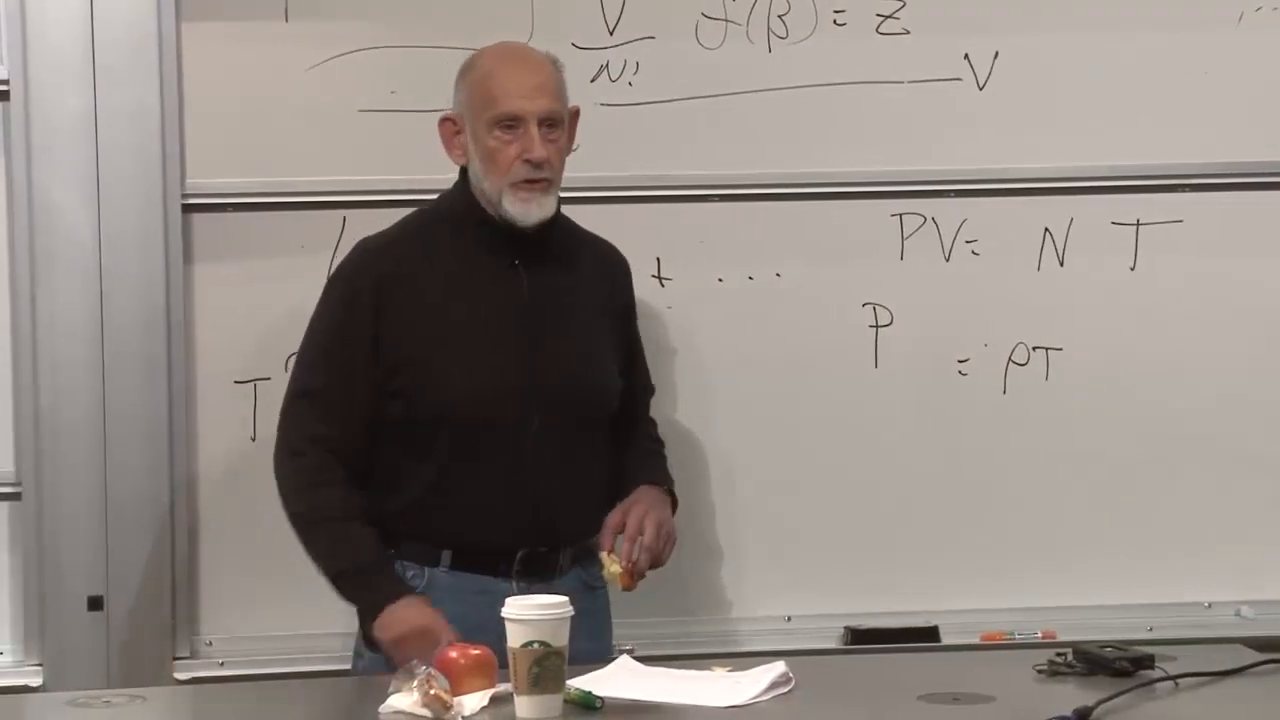
\includegraphics[width=0.90\textwidth]{lecture_05_figure_08.png}
\caption{\(\log Z\)的体积导数以及由此得到的理想气体状态方程\(PV=NT\)，或\(P=\rho T\)。}
\lectureframe{01:09:25}
\end{figure}

恢复实验室温度\(T_K\)，
\begin{equation}
 PV=Nk_BT_K.
 \label{eq:sm5-ideal-gas-law-laboratory}
\end{equation}
这个熟悉的结果与动理学直觉一致，但它的推导现在建立在一个远远超出自由气体的框架之上。

\section{第二个收获：平衡涨落}

压强计算已经完成，但还有一个承诺过的问题：还能从配分函数中提取什么？考虑一个与热浴热接触的系统。它的能量并不固定。能量进入和离开，因此重复测量会在正则平均值附近涨落。

\begin{classroomqa}
\audiencequestion{我们现在能计算之前承诺的涨落吗？}
\lecturerresponse{能。额外的时间允许对同一原理进行第二次演示：\(Z\)的导数编码了可测量的热力学信息。
\lecturetimestamp{01:10:37--01:10:50}}
\end{classroomqa}

\subsection{方差与标准差}

对于随机变量\(x\)，其中\(\langle x\rangle=0\)，分布宽度的一种度量是\(\langle x^2\rangle\)。对于一般分布，将变量平移其均值：
\begin{equation}
 \delta x=x-\langle x\rangle.
 \label{eq:sm5-centered-variable}
\end{equation}
它的均值为零，
\begin{equation}
 \langle\delta x\rangle
 =
 \langle x\rangle-\langle x\rangle=0,
 \label{eq:sm5-centered-mean}
\end{equation}
其均方为
\begin{align}
 (\Delta x)^2
 &\equiv
 \left\langle\left(x-\langle x\rangle\right)^2\right\rangle \notag\\
 &=
 \langle x^2\rangle
 -2\langle x\rangle^2
 +\langle x\rangle^2 \notag\\
 &=
 \langle x^2\rangle-\langle x\rangle^2.
 \label{eq:sm5-variance}
\end{align}
这就是方差。它的正平方根\(\Delta x\)是标准差。

\begin{classroomqa}
\audiencequestion{为什么
\(x-\langle x\rangle\)的平均值恰好为零？}
\lecturerresponse{平均是线性的，而\(\langle x\rangle\)已经是一个数。因此
\(\langle x-\langle x\rangle\rangle
=\langle x\rangle-\langle x\rangle=0\)。
\lecturetimestamp{01:14:02--01:14:22}}
\end{classroomqa}

\begin{classroomqa}
\audiencequestion{平方涨落、方差、均方根宽度和标准差之间有什么区别？}
\lecturerresponse{方差是
\((\Delta x)^2=\langle x^2\rangle-\langle x\rangle^2\)。
标准差是它的平方根，\(\Delta x\)。对于零均值变量，标准差也是它的均方根值。
\lecturetimestamp{01:16:39--01:18:38}}
\end{classroomqa}

\begin{figure}[t]
\centering
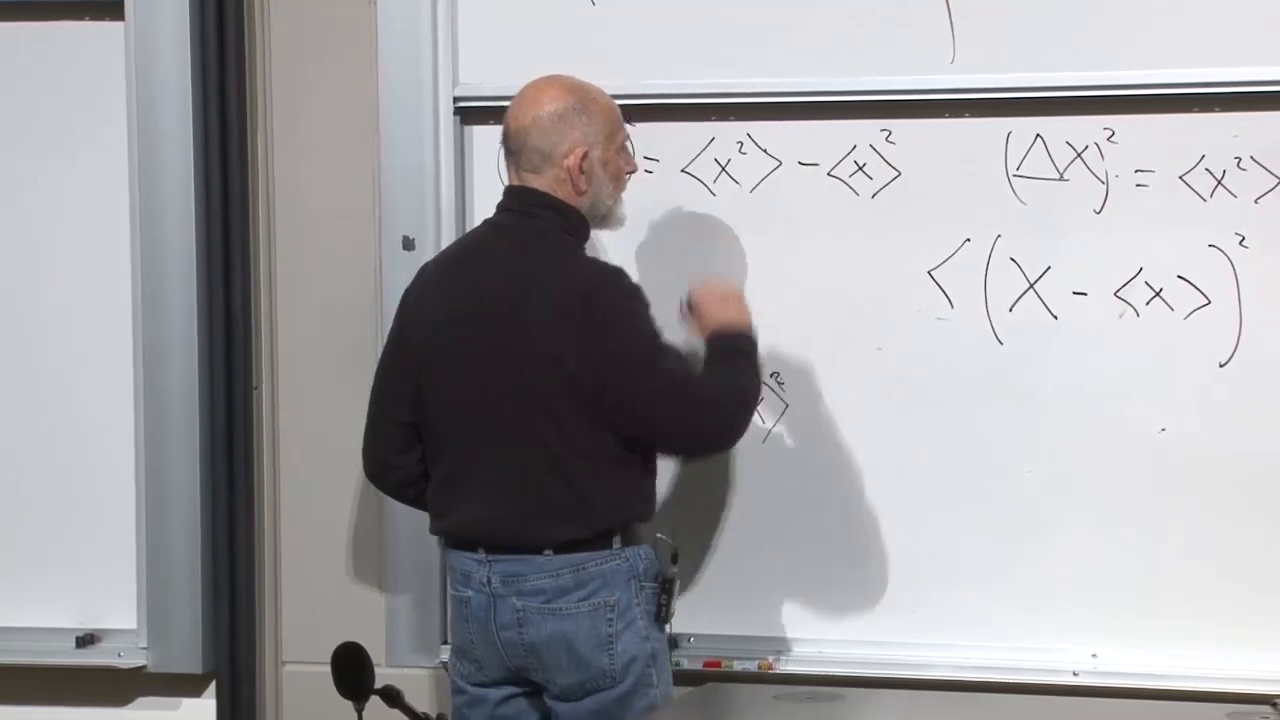
\includegraphics[width=0.90\textwidth]{lecture_05_figure_09.png}
\caption{平移后的变量以及产生\((\Delta x)^2=\langle x^2\rangle-\langle x\rangle^2\)的展开。}
\lectureframe{01:17:20}
\end{figure}

\subsection{由配分函数得到的能量矩}

对于正则系综，
\begin{align}
 \langle E\rangle
 &=
 \frac{1}{Z}\sum_i E_i e^{-\beta E_i} \notag\\
 &=
 -\frac{1}{Z}\frac{\partial Z}{\partial\beta}
 =
 -\frac{\partial\log Z}{\partial\beta}.
 \label{eq:sm5-mean-energy-from-z}
\end{align}
乘以一个\(E_i\)因子由一个负\(\beta\)导数产生。二阶导数生成\(E_i^2\)：
\begin{equation}
 \langle E^2\rangle
 =
 \frac{1}{Z}\sum_i E_i^2e^{-\beta E_i}
 =
 \frac{1}{Z}\frac{\partial^2 Z}{\partial\beta^2}.
 \label{eq:sm5-second-energy-moment}
\end{equation}
因此能量方差为
\begin{align}
 (\Delta E)^2
 &=
 \langle E^2\rangle-\langle E\rangle^2 \notag\\
 &=
 \frac{1}{Z}\frac{\partial^2Z}{\partial\beta^2}
 -
 \frac{1}{Z^2}
 \left(\frac{\partial Z}{\partial\beta}\right)^2 \notag\\
 &=
 \frac{\partial^2\log Z}{\partial\beta^2}
 =
 -\frac{\partial\langle E\rangle}{\partial\beta}.
 \label{eq:sm5-energy-variance-beta}
\end{align}
再一次，一个看起来复杂的可观测量变成了\(\log Z\)的导数。

\begin{figure}[t]
\centering
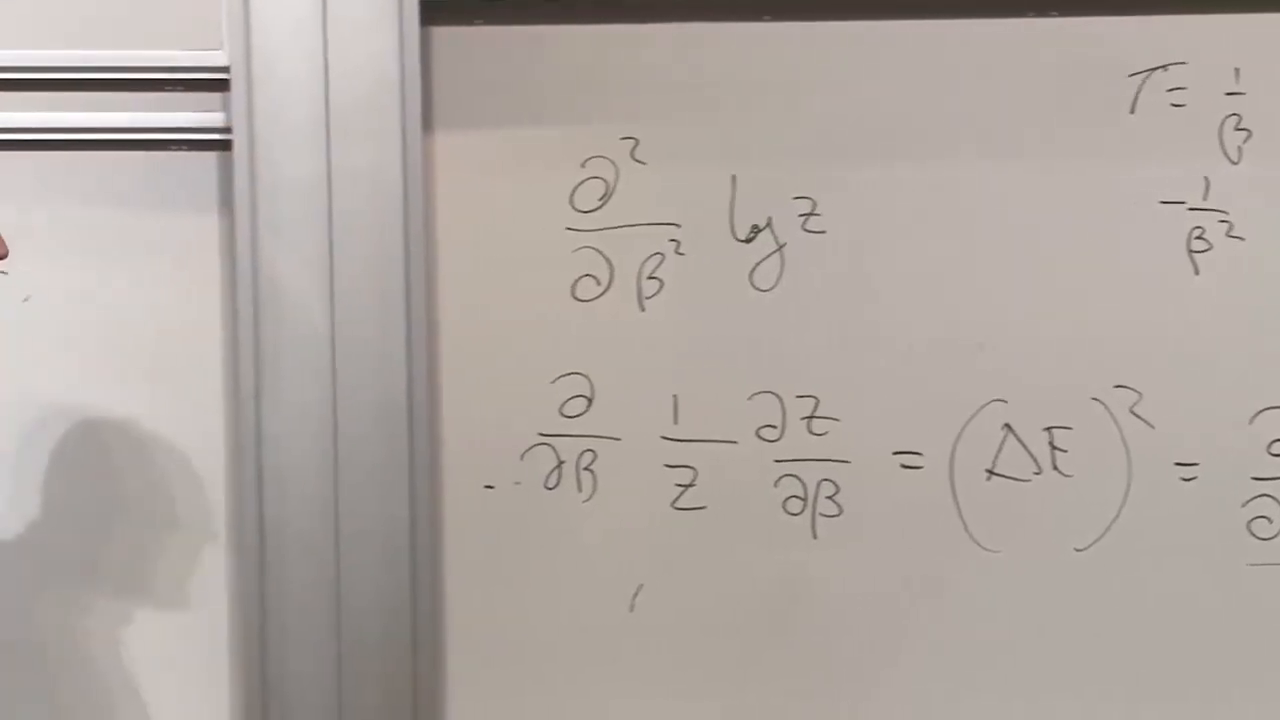
\includegraphics[width=0.90\textwidth]{lecture_05_figure_10.png}
\caption{\(\log Z\)的二阶\(\beta\)导数被等同于能量方差。}
\lectureframe{01:29:00}
\end{figure}

\subsection{热容与涨落的大小}

在讲义单位中\(T=1/\beta\)，所以
\begin{equation}
 -\frac{\partial}{\partial\beta}
 =
 T^2\frac{\partial}{\partial T}.
 \label{eq:sm5-beta-temperature-derivative}
\end{equation}
在固定体积下，定义整个样本的热容为
\begin{equation}
 C_V\equiv
 \left(\frac{\partial\langle E\rangle}{\partial T}\right)_V.
 \label{eq:sm5-heat-capacity}
\end{equation}
方程\eqref{eq:sm5-energy-variance-beta}变为
\begin{equation}
 \boxed{(\Delta E)^2=T^2C_V}
 \qquad (k_B=1).
 \label{eq:sm5-energy-fluctuation-lecture-units}
\end{equation}
对于实验室温度\(T_K\)，其中
\(\beta=(k_BT_K)^{-1}\)，
\begin{equation}
 \boxed{(\Delta E)^2=k_BT_K^2C_V}.
 \label{eq:sm5-energy-fluctuation-laboratory}
\end{equation}

\begin{figure}[t]
\centering
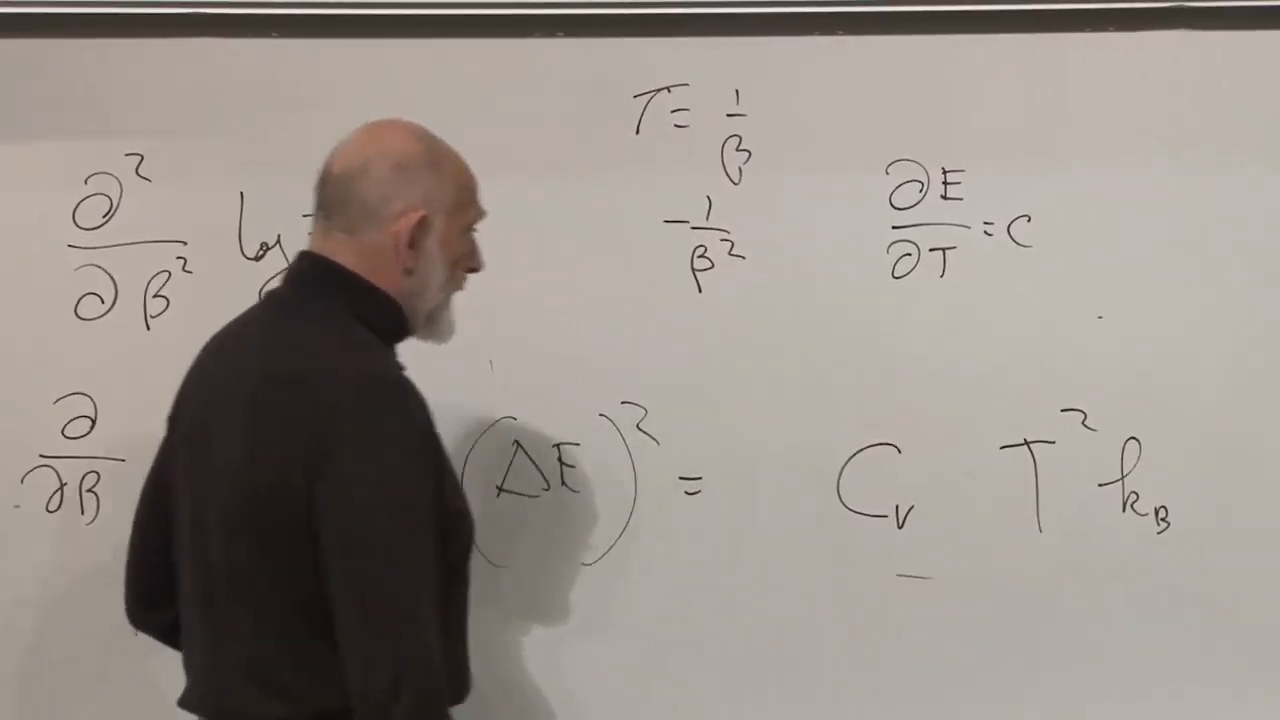
\includegraphics[width=0.90\textwidth]{lecture_05_figure_11.png}
\caption{从\(\beta\)导数到定容热容的转换，其中恢复了\(k_B\)因子。}
\lectureframe{01:31:10}
\end{figure}

\begin{classroomqa}
\audiencequestion{该导数必须指定固定体积而非固定压强吗？}
\lecturerresponse{是的。这一正则推导保持哈密顿量的外部控制参数固定，其中包括\(V\)。所得的量是\(C_V\)。定压系综允许体积和功发生涨落，并需要相应的热力学势；不能简单地在\eqref{eq:sm5-energy-fluctuation-laboratory}中把\(C_V\)替换为\(C_P\)。
\lecturetimestamp{01:29:01--01:29:28; 01:32:50--01:33:21}}
\end{classroomqa}

\begin{classroomqa}
\audiencequestion{\(C_V\)是材料常数吗？}
\lecturerresponse{一般而言不是。它可能依赖于温度、体积、相和组成。此外，这里的\(C_V\)是整个样品的热容，是广延量。只有除以质量、粒子数或物质的量之后，才得到比热。
\lecturetimestamp{01:31:47--01:32:21; 01:33:23--01:34:55}}
\end{classroomqa}

对于普通的广延物质，\(C_V\)正比于\(N\)，因此\((\Delta E)^2\)正比于\(N\)，而\(\Delta E\)正比于\(\sqrt{N}\)。平均能量本身正比于\(N\)。因此
\begin{equation}
 \frac{\Delta E}{\langle E\rangle}\sim\frac{1}{\sqrt{N}}.
 \label{eq:sm5-relative-fluctuation-scaling}
\end{equation}
宏观相对涨落极小，而微观样品则直接显示出这些涨落。\(k_B\)出现在\eqref{eq:sm5-energy-fluctuation-laboratory}中，标志着热力学可观测量与分子离散性之间的这种联系；等价地说，它把宏观单位与阿伏伽德罗尺度的计数联系起来。

压强和涨落现在已从同一个对象中涌现出来：
\[
 P=T\left(\frac{\partial\log Z}{\partial V}\right)_T,
 \qquad
 (\Delta E)^2=\frac{\partial^2\log Z}{\partial\beta^2}.
\]
这就是核心教训。一旦确定了正确的约束，配分函数就不仅仅是对概率进行归一化。它的导数组织起系统可测量的热力学。
\chapter{弱相互作用、维里修正与非恰当微分}

\lectureoverview{我们首先讨论测量与温度的操作性含义，然后追问当短程相互作用被微弱地开启时，稀薄气体如何偏离理想气体定律。配分函数给出能量与压强的首批相互作用修正，并确定其适用范围。最后的数学插曲借助恰当微分、闭合回路以及一个具体的理想气体检验，把态函数与路径依赖的热和功区分开来。}

\section{仪器实际测量的是什么}

没有任何实验室装置能直接伸入自然之中并报告一个抽象的数学变量。弹簧秤报告的是伸长量；温度计报告的是液柱高度。我们之所以把前者称为力的测量、把后者称为温度的测量，只是因为已经在可见响应与所需量之间建立起了一种可重复的关系。

这种关系有其有限的适用范围。弹簧只有在保持弹性时才服从胡克定律，而足够大的力最终会使其变形或断裂。更一般地，若一个光滑的读数\(R\)依赖于物理变量\(X\)，则在选定的工作点附近有
\begin{equation}
 \Delta R \simeq
 \left.\frac{dR}{dX}\right|_{X_0}\Delta X.
 \label{eq:sm6-local-linear-response}
\end{equation}
即使完整的响应曲线是非线性的，读数的小变化也与目标变量的小变化成正比。这种局部线性化正是校准的通常逻辑。

读数还可能依赖于干扰变量。弹簧可能对温度或压强有微弱的响应。温度计中水银柱的高度可能通过重力而随取向变化，也可能受玻璃性质或材料缓慢变化的影响。测量方案并不证明这些依赖关系不存在；它只是把它们固定住，或表明它们在所需尺度上可以忽略。

\begin{classroomqa}
\audiencequestion{局部引力场，或者温度计被拿持的方向，会不会改变读数？}
\lecturerresponse{原则上会。如果取向有可观的影响，那么竖直拿持温度计这一指令就成为该仪器定义的一部分。在地球表面附近，引力场足够稳定，剩余的变化通常可以忽略。
\lecturetimestamp{00:04:08--00:05:00}}
\end{classroomqa}

\begin{classroomqa}
\audiencequestion{老化或化学变化会不会缓慢地改变校准？}
\lecturerresponse{有可能。对于普通测量而言，水银和玻璃足够惰性，而在极其漫长的时间尺度上的变化与实验无关。校准始终是关于指定仪器、范围、方案和持续时间的陈述。
\lecturetimestamp{00:05:03--00:06:11}}
\end{classroomqa}

对于摄氏温度计，两个可重复的参考状态提供了一个方便的标度。若\(h_f\)和\(h_b\)分别是水在凝固点和沸点时的液柱高度，则在响应近似线性的范围内有
\begin{equation}
 T_{\mathrm C}=100\,\frac{h-h_f}{h_b-h_f}.
 \label{eq:sm6-celsius-calibration}
\end{equation}
在凝固点取\(T_{\mathrm C}=0\)是一种约定。它并不是热能为零的状态，正如冬日里华氏零度并非绝对零度。

\begin{figure}[t]
\centering
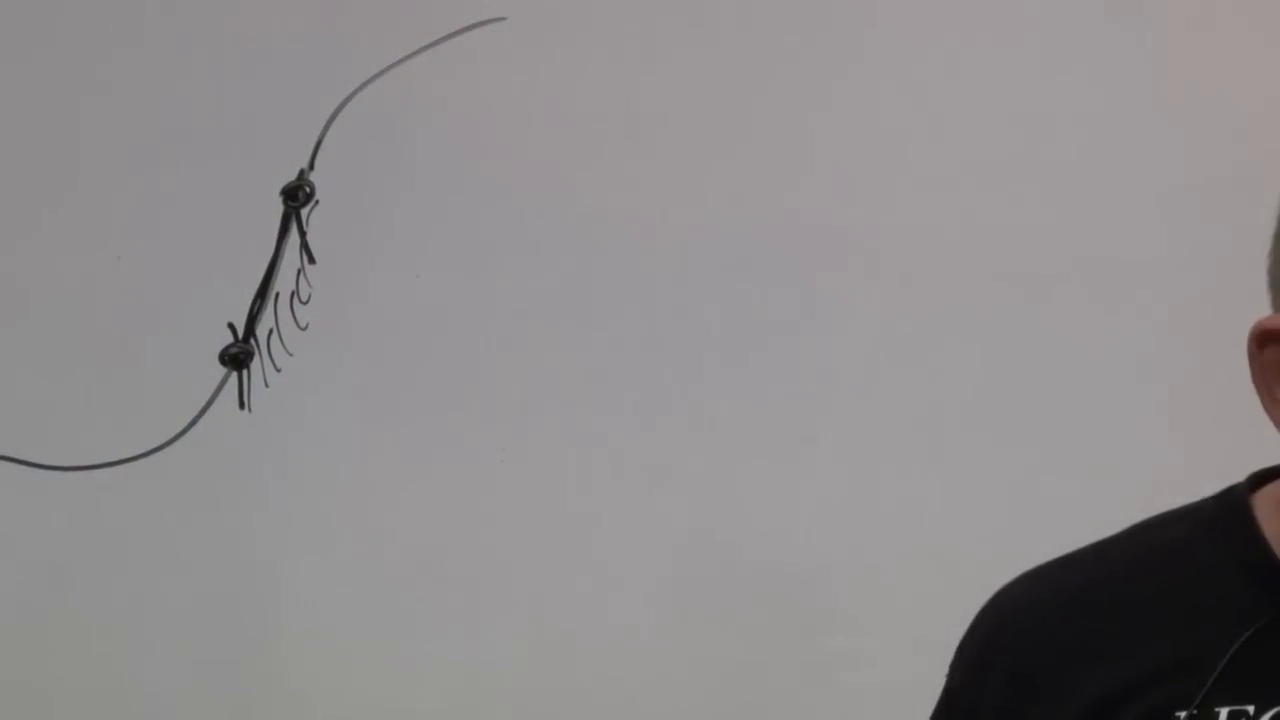
\includegraphics[width=0.90\textwidth]{lecture_06_figure_03.png}
\caption{一个光滑但非线性的温度计响应，其中标出了一段短区间用于线性校准。}
\lectureframe{00:07:55}
\end{figure}

\section{平衡与作为能量标度的温度}

只有当温度计与附近介质达到热平衡之后，温度计测量的才是其环境的温度。在此之前，它的读数只是在朝着平衡变化。实用的检验很简单：等到读数不再变化为止。这条规则的简单性掩盖了决定等待时间的那些物理过程。

\begin{classroomqa}
\audiencequestion{达到平衡是否只涉及球泡周围的一层边界层，又应当等待多久？}
\lecturerresponse{能量必须穿过玻璃并与周围介质交换，因此时间取决于温度计、其热导率以及介质。紧邻的环境还必须能代表一个均匀的平衡态。在实验上，当读数不再漂移时，就认为可以接受。
\lecturetimestamp{00:08:45--00:10:13}}
\end{classroomqa}

在这一等待时间中，温度与密度扮演着不同的角色。非常稀薄的气体可以非常热：其中为数不多的分子可能带有很大的动能。然而这些分子很少撞击温度计，因此达到平衡可能很慢。在保持温度不变的情况下把密度降低一百倍或一千倍，并不会降低分子的能量标度；它降低的是该能量被传递给仪器的速率。

\begin{classroomqa}
\audiencequestion{房间里的辐射温度可以不同于空气的温度吗？}
\lecturerresponse{可以。物质与辐射只有在彼此处于热平衡时才共享同一个温度。中性空气与照明房间中大部分光学辐射的耦合很弱，因此光子布居不必是处于空气温度下的平衡黑体场。
\lecturetimestamp{00:11:26--00:12:20}}
\end{classroomqa}

一旦建立平衡，温度最好被视为一种能量标度。我们继续使用\(k_B=1\)的单位制，因此\(T\)本身具有能量的量纲。对于单原子理想气体，
\begin{equation}
 E_0=\frac{3}{2}NT.
 \label{eq:sm6-ideal-energy}
\end{equation}
每个分子的热能由\(T\)固定；相应的速率仍然依赖于分子质量。

\section{开启弱相互作用}

\begin{classroomqa}
\audiencequestion{在什么条件下理想气体近似会失效，并且这种失效能否用数学方式展示？}
\lecturerresponse{从已求解的非相互作用气体出发，开启一个小的相互作用。按该变化量展开，计算第一阶修正，并将其与理想项比较。当修正不再小时，该近似失效。
\lecturetimestamp{00:12:25--00:14:40}}
\end{classroomqa}

这是标准的微扰策略。如果一个问题在\(\lambda=0\)时可解，就引入耦合\(\lambda\)，写出
\begin{equation}
 F(\lambda)=F(0)+\lambda F_1+\lambda^2F_2+\cdots,
 \label{eq:sm6-perturbative-template}
\end{equation}
并追问所保留的每一项是否都小于前一项。这里的参考问题是理想气体。物理上的小量来自稀薄的样品、比平均间距短的相互作用程，以及足够弱、使第一阶相互作用项有用的势。高密度或长程力可能使该近似失效，即使任何一次相遇看起来都很温和。

设\(x_i\in\mathbb R^3\)和\(p_i\in\mathbb R^3\)分别为分子\(i\)的位置和动量。对于质量为\(m\)的全同分子，取
\begin{equation}
 H(X,P)=
 \sum_{i=1}^{N}\frac{p_i^2}{2m}
 +\sum_{i<j}u\!\left(|x_i-x_j|\right),
 \label{eq:sm6-interacting-hamiltonian}
\end{equation}
其中\(X=(x_1,\ldots,x_N)\)，\(P=(p_1,\ldots,p_N)\)。限制条件\(i<j\)排除了自身配对，并且只将\((i,j)\)计数一次：
\begin{equation}
 \sum_{i<j}1=\binom{N}{2}=\frac{N(N-1)}{2}.
 \label{eq:sm6-pair-count}
\end{equation}

\begin{classroomqa}
\audiencequestion{为什么不分别对两个粒子标签独立求和？}
\lecturerresponse{对\((3,7)\)与对\((7,3)\)是同一个物理对，而且粒子不会与自身配对。将求和限制在\(i<j\)同时强制了这两个事实。质量符号保留为\(m\)，而\(i,j\)用于标记粒子，以避免当\(m\)被同时用于这两种用途时可能出现的记号冲突。
\lecturetimestamp{00:17:52--00:19:12}}
\end{classroomqa}

将总构型势写为
\begin{equation}
 U(X)=\sum_{i<j}u\!\left(|x_i-x_j|\right).
 \label{eq:sm6-total-potential}
\end{equation}
假定相互作用具有平移不变性且为短程：当\(r\)与分子长度相比很大时，\(u(r)\)变得可忽略。

\section{积分后的对强度}

只有弱对势的一个积分进入第一阶修正：
\begin{equation}
 U_0\equiv\int_{\mathbb R^3}d^3r\,u(r).
 \label{eq:sm6-u0-definition}
\end{equation}
其单位是能量乘以体积。它把相互作用的典型强度与该相互作用可观的体积结合起来。

\begin{figure}[t]
\centering
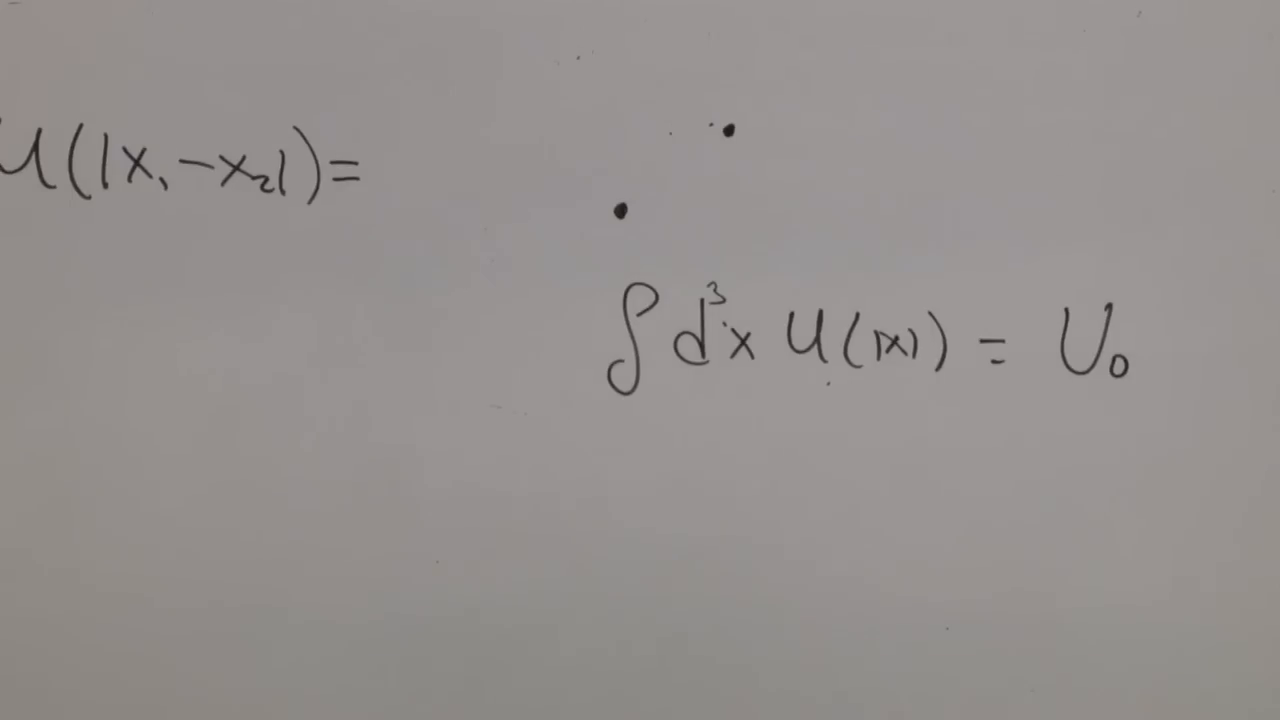
\includegraphics[width=0.90\textwidth]{lecture_06_figure_04.png}
\caption{短程对势被压缩为积分强度\(U_0=\int d^3r\,u(r)\)。}
\lectureframe{00:25:15}
\end{figure}

为了看清\(U_0\)为何有用，考虑一个对：
\begin{equation}
 I_2=\int_V d^3x_1\,d^3x_2\,
 u\!\left(|x_1-x_2|\right).
 \label{eq:sm6-two-particle-integral}
\end{equation}
引入相对坐标\(r=x_2-x_1\)。远离边界时，相对积分给出\(U_0\)，而该对的共同位置则遍历整个容器。因此
\begin{equation}
 I_2=V U_0+\text{surface corrections}.
 \label{eq:sm6-pair-integral-vu0}
\end{equation}
修正来自距壁面一个相互作用程内的粒子，此时相对坐标邻域的一部分位于盒子之外。其相对重要性按表面积与体积之比标度，并在宏观极限下消失。

\begin{classroomqa}
\audiencequestion{\(U_0\)指的是某个选定的对，并且是否让一个粒子与另一个粒子保持固定间距？}
\lecturerresponse{它指的是任意一个对所遵循的共同相互作用规律。将第一个粒子固定，对第二个粒子的所有相对位置积分。在此积分过程中间距并不固定。只有附近的相互作用区域有可观贡献，从而产生\(U_0\)。
\lecturetimestamp{00:26:03--00:27:33}}
\end{classroomqa}

\begin{classroomqa}
\audiencequestion{为什么第二个位置积分给出整个容器的体积，而第一个不给出？}
\lecturerresponse{在相对构型被积分成\(U_0\)之后，整个对可以在样品中平移。这种共同平移提供了大因子\(V\)。相互作用邻域是一个分子尺度的体积，已经包含在\(U_0\)之内，而不是另一个等于容器体积的因子。
\lecturetimestamp{00:27:48--00:29:21}}
\end{classroomqa}

\begin{classroomqa}
\audiencequestion{这个值会不会依赖于固定的是哪个点，尤其是在壁面附近？}
\lecturerresponse{平移不变性使得体相值与固定点无关。在壁面附近，积分会略有不同，因为有些邻近位置不可用。只有分子厚度的表面层受到影响，因此当盒子是宏观尺度时，误差可以忽略。
\lecturetimestamp{00:29:24--00:31:22}}
\end{classroomqa}

\begin{classroomqa}
\audiencequestion{结果是不是对每一个两粒子构型积分后的势能，为什么它只正比于一个大的体积？}
\lecturerresponse{是的。它的单位是能量乘以体积的平方，因为\(V U_0\)包含一个容器体积和一个分子相互作用体积。其中只有前者随样品尺寸增大。
\lecturetimestamp{00:31:31--00:32:04}}
\end{classroomqa}

\begin{classroomqa}
\audiencequestion{选择在固定体积下面积最小的球，会改变体相答案吗？}
\lecturerresponse{它只改变很小的边界修正。对于任何普通的宏观形状，距表面一个分子距离内的粒子数与体相中的粒子数相比可以忽略。只有当容器本身接近分子尺度时，表面才变得重要。
\lecturetimestamp{00:32:04--00:33:58}}
\end{classroomqa}

\begin{classroomqa}
\audiencequestion{用势代替粒子轨迹，是否就把碰撞省略掉了？}
\lecturerresponse{没有。力是势的导数，正是它产生碰撞。平衡态统计力学并不要求我们逐一追踪这些碰撞；它们的效果被编码在能量中，因而也编码在玻尔兹曼权重中。
\lecturetimestamp{00:33:59--00:35:29}}
\end{classroomqa}

\begin{classroomqa}
\audiencequestion{保留对力而不保留真正的三体相互作用，会损失什么？}
\lecturerresponse{微观能量可以包含真正的三体项，而对势的高阶项也会产生多粒子关联。然而在稀薄气体中，指定的三个粒子占据同一个分子邻域的可能性远小于两个粒子。因此对效应给出第一阶密度修正；更高的集团项以更高阶的密度幂次进入。
\lecturetimestamp{00:35:29--00:38:14}}
\end{classroomqa}

\section{自动运行下的配分函数}

统计方法的优势现在显现出来了。一旦哈密顿量给定，就无需猜测壁面附近或碰撞过程中的详细速度分布。我们写出正则配分函数并遵循其代数运算：
\begin{equation}
\begin{aligned}
 Z&=
 \frac{1}{N!h^{3N}}
 \int d^{3N}P\,d^{3N}X\\
 &\qquad{}\times e^{-\beta K(P)}e^{-\beta U(X)},\\
 K(P)&=\sum_i\frac{p_i^2}{2m}.
\end{aligned}
 \label{eq:sm6-full-partition-function}
\end{equation}
因子\(h^{3N}\)使经典相空间测度无量纲化，而\(N!\)消除了全同粒子的置换重复计数。

\begin{figure}[t]
\centering
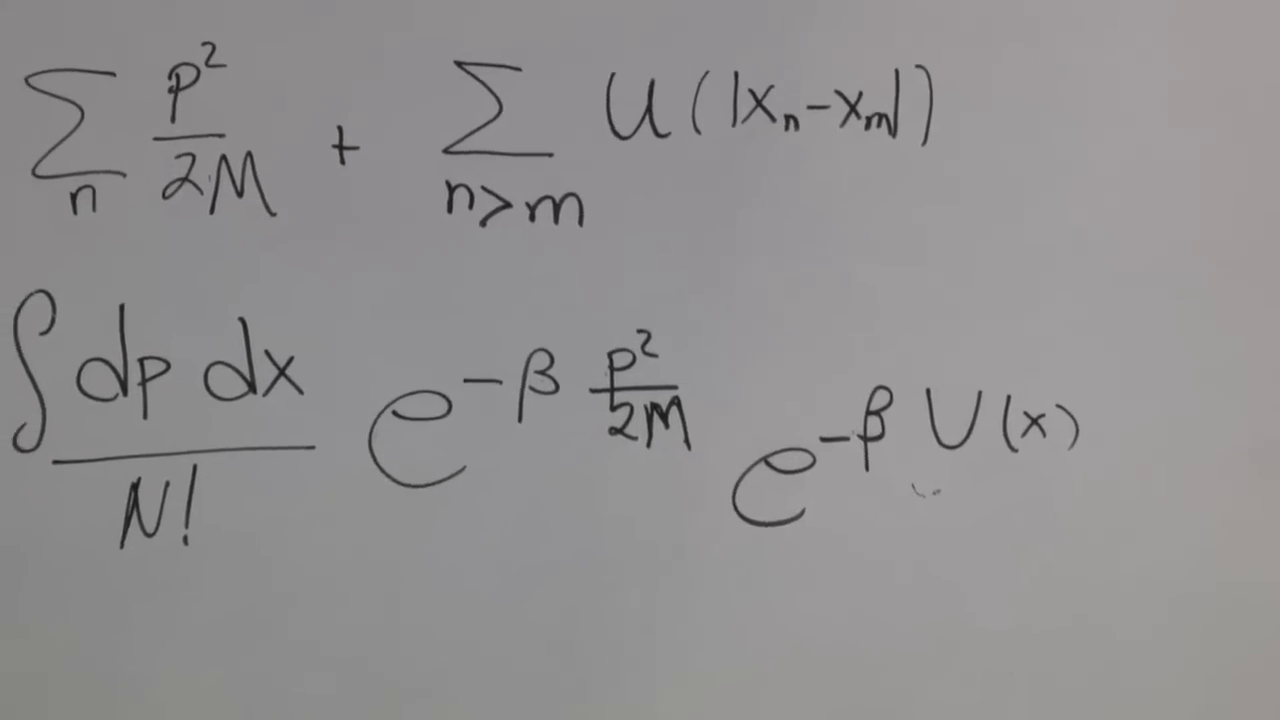
\includegraphics[width=0.90\textwidth]{lecture_06_figure_05.png}
\caption{多粒子能量以及配分函数中相应的动能因子和构型因子。}
\lectureframe{00:40:35}
\end{figure}

动量与位置分离。将构型积分乘以并除以\(V^N\)，即可分离出理想气体结果：
\begin{align}
 Z
 &=\left[
 \frac{V^N}{N!h^{3N}}
 \int d^{3N}P\,e^{-\beta K(P)}
 \right] \notag\\
 &\quad\times\left[
 \frac{1}{V^N}
 \int d^{3N}X\,e^{-\beta U(X)}
 \right] \notag\\
 &\equiv Z_0\,C(\beta,V,N).
 \label{eq:sm6-z-factorization}
\end{align}
熟悉的高斯因子为
\begin{equation}
 \int d^{3N}P\,e^{-\beta K(P)}
 =\left(\frac{2\pi m}{\beta}\right)^{3N/2}.
 \label{eq:sm6-gaussian-factor}
\end{equation}

\begin{figure}[t]
\centering
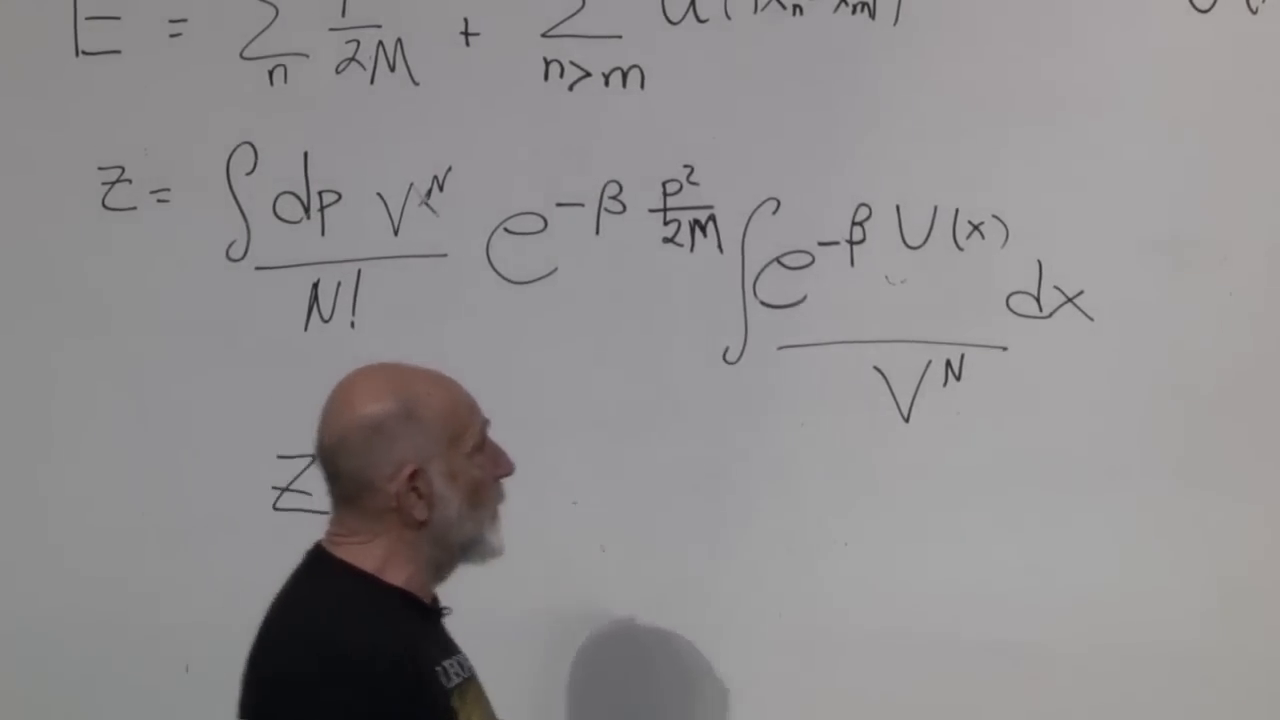
\includegraphics[width=0.90\textwidth]{lecture_06_figure_06.png}
\caption{从归一化构型因子中分离出的理想气体配分函数。}
\lectureframe{00:43:45}
\end{figure}

因子\(N!\)不影响归一化比值\(C\)，也不影响下文所用的特定固定\(N\)导数，但它并非可以从整体热力学中省略：它对于正确的状态计数和广延熵是必不可少的。

到相互作用的一阶，
\begin{equation}
 e^{-\beta U(X)}
 =1-\beta U(X)+O(U^2).
 \label{eq:sm6-boltzmann-expansion}
\end{equation}
因此，
\begin{align}
 C
 &=
 1-\frac{\beta}{V^N}
 \sum_{i<j}
 \int d^{3N}X\,u(|x_i-x_j|)
 +O(U^2) \notag\\
 &=
 1-\frac{\beta}{V^N}
 \frac{N(N-1)}{2}
 V^{N-2}(V U_0)+O(U^2) \notag\\
 &=
 1-\beta\frac{N(N-1)}{2V}U_0+O(U^2).
 \label{eq:sm6-configurational-correction}
\end{align}
每一对都有相同的\emph{积分}，而不是相同的瞬时间距或势能。剩余的\(N-2\)个位置积分各贡献一个\(V\)因子。

\begin{figure}[t]
\centering
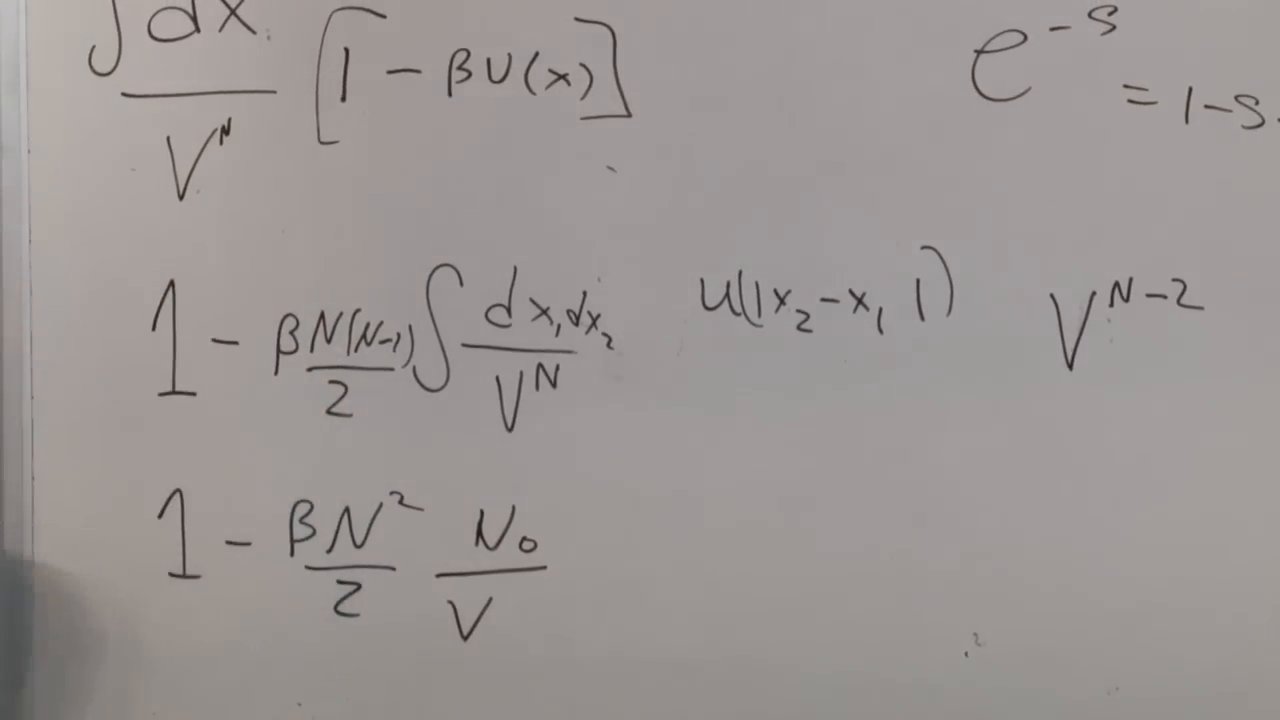
\includegraphics[width=0.90\textwidth]{lecture_06_figure_07.png}
\caption{对计数、旁观者坐标体积以及第一阶构型修正\(1-\beta N^2U_0/(2V)\)。}
\lectureframe{00:53:40}
\end{figure}

\begin{classroomqa}
\audiencequestion{领头项\(1\)是否假设势在零间距处为零？}
\lecturerresponse{不是。它是指数级数中的零阶项，与\(u(0)\)的值无关。势出现在下一项\(-\beta U(X)\)中。
\lecturetimestamp{00:46:19--00:46:48}}
\end{classroomqa}

\begin{classroomqa}
\audiencequestion{如果不同的对有不同的间距，为什么每一对都可以用同一个表达式代替？}
\lecturerresponse{并不是把它们的逐点值等同起来。每一项都在同一个完整构型空间上积分，而粒子标签并不区分这一对和那一对。这些积分具有相同的形式和相同的值。
\lecturetimestamp{00:50:00--00:51:07}}
\end{classroomqa}

\begin{classroomqa}
\audiencequestion{配对数究竟是\(N(N-1)/2\)还是
\(N(N+1)/2\)？}
\lecturerresponse{是\(N(N-1)/2\)：选定一个粒子后，只有\(N-1\)个不同的伙伴，而除以二则去除了反向的排序。对于宏观的\(N\)，将\(N(N-1)\)替换为\(N^2\)只改变一个相对的\(1/N\)修正。
\lecturetimestamp{00:48:33--00:49:56}}
\end{classroomqa}

由于\(\log(1-x)=-x-x^2/2-x^3/3-\cdots\)不是交错级数，一阶对数项为
\begin{equation}
 \log Z
 =
 \log Z_0
 -\beta\frac{N(N-1)}{2V}U_0
 +O(U^2).
 \label{eq:sm6-logz-correction}
\end{equation}
在\(N\)很大时，我们可以将\(N(N-1)\)替换为\(N^2\)，此时不需要有限\(N\)的区分。

\begin{remark}
受控的低密度表述使用Mayer函数
\(f(r)=e^{-\beta u(r)}-1\)以及第二维里系数
\begin{equation}
 B_2(T)=-\frac{1}{2}\int d^3r\,f(r).
 \label{eq:sm6-second-virial}
\end{equation}
对于弱势，\(f(r)\simeq-\beta u(r)\)，因此
\(B_2\simeq\beta U_0/2\)，从而重新得到下面的结果。对于硬排斥核心，这一形式是必需的，因为直接展开\(e^{-\beta u}\)并不成立。
\end{remark}

\section{能量、压强以及修正的含义}

\(Z\)的对数之所以有用，是因为它的导数是可以测量的。假设微观势与温度无关，
\begin{align}
 E
 &=-\left(\frac{\partial\log Z}{\partial\beta}\right)_{V,N} \notag\\
 &=
 \frac{3}{2}NT
 +\frac{N(N-1)}{2V}U_0+O(U^2) \notag\\
 &\simeq
 N\left(\frac{3}{2}T+\frac{1}{2}\rho U_0\right),
 \qquad
 \rho=\frac{N}{V}.
 \label{eq:sm6-energy-correction}
\end{align}
表面上非广延的\(N^2\)伴随着\(1/V\)。在固定密度下，\(N^2/V=N\rho\)，因此总能量仍然与系统的尺度成正比。每个粒子的额外能量与密度成正比，因为一个被选定的分子只有在另一个分子位于附近时才会获得对能量。

\begin{figure}[t]
\centering
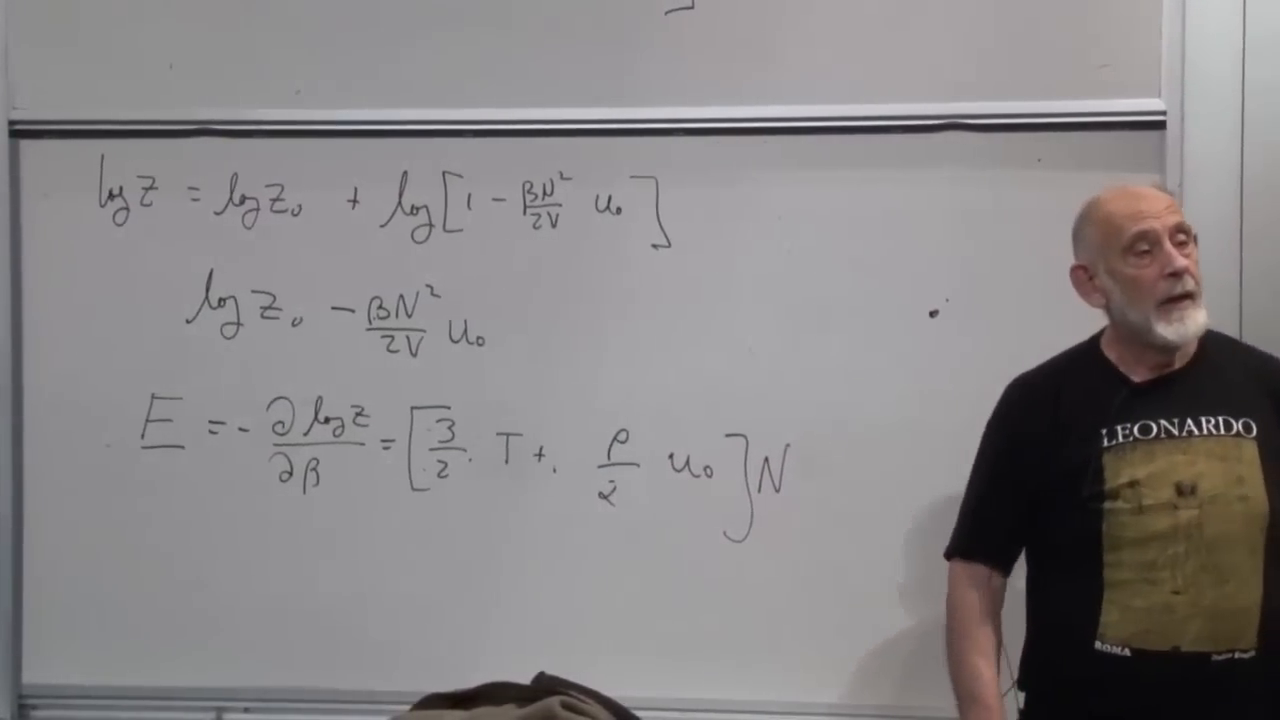
\includegraphics[width=0.90\textwidth]{lecture_06_figure_08.png}
\caption{第一项相互作用修正被重新组织为广延能量\(N[3T/2+\rho U_0/2]\)。}
\lectureframe{01:03:25}
\end{figure}

压强更容易测量。利用上一章的结果，
\begin{equation}
 P=T\left(\frac{\partial\log Z}{\partial V}\right)_{T,N},
 \label{eq:sm6-pressure-from-z}
\end{equation}
我们得到
\begin{align}
 P
 &=
 \frac{NT}{V}
 +T\frac{\partial}{\partial V}
 \left(-\beta\frac{N(N-1)}{2V}U_0\right)
 +O(U^2) \notag\\
 &=
 \rho T+\frac{1}{2}\rho^2U_0
 +O\!\left(\frac{\rho U_0}{N},U^2\right).
 \label{eq:sm6-pressure-correction}
\end{align}

\begin{figure}[t]
\centering
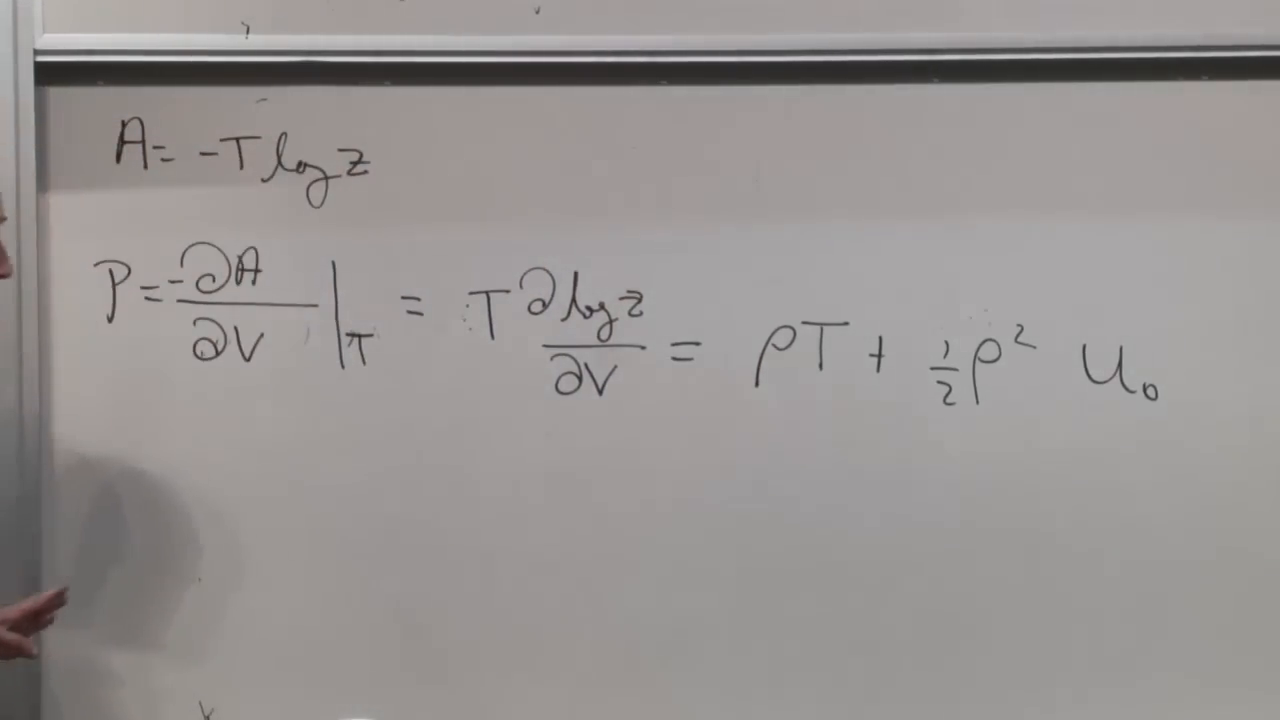
\includegraphics[width=0.90\textwidth]{lecture_06_figure_09.png}
\caption{由Helmholtz导数得到的压强，包含第一个二次密度修正。}
\lectureframe{01:09:50}
\end{figure}

\begin{classroomqa}
\audiencequestion{为什么\(\rho^2\)，而不是另一个幂次，才是自然的第一项修正？}
\lecturerresponse{理想项要求有一个粒子出现在一个小区域内，因此按\(\rho\)标度。相互作用则要求有两个粒子占据同一个分子邻域，其概率按\(\rho^2\)标度。因子\(1/2\)正是那个配对计数因子，它防止\((i,j)\)和\((j,i)\)被分别计数。
\lecturetimestamp{01:24:27--01:26:00}}
\end{classroomqa}

在固定温度下，可以改变\(V\)，测量\(\rho=N/V\)，并绘制压强。理想定律是线性项。\(P(\rho)\)的曲率揭示了第一项相互作用修正。在这个弱势近似内，该修正没有显式的温度依赖，因为\eqref{eq:sm6-pressure-from-z}中的因子\(T\)与\(\beta=1/T\)相消。

\begin{classroomqa}
\audiencequestion{密度可以增大到多大，才必须包含三体效应？}
\lecturerresponse{密度计数表明，下一个维里项与\(\rho^3\)成正比，但仅凭\(U_0\)无法推断其系数。它来自对相互作用的关联乘积的贡献，以及如果存在的话，真正的三体力。必须计算下一个集团系数，并将其与\(\rho^2\)项比较；不应把猜测的公式提升为结果。
\lecturetimestamp{01:10:50--01:13:38}}
\end{classroomqa}

当修正的幅度很小时，理想气体项占主导：
\begin{equation}
 \begin{aligned}
 \frac{1}{2}\rho^2|U_0|&\ll \rho T,\\
 |\rho U_0|&\ll T
 \qquad\text{(parametrically)}.
 \end{aligned}
 \label{eq:sm6-ideal-validity}
\end{equation}
第二个不等式的两边都是能量。量\(\rho U_0\)是每个粒子的相互作用能量尺度，而\(T\)是动能尺度。普通的稀薄室温气体远处于这一区域内；只有当分子邻域被占据得足够频繁，使相互作用足以与热运动相竞争时，才会出现显著的偏离。

\begin{classroomqa}
\audiencequestion{这个判据能对房间里的空气进行估计吗？}
\lecturerresponse{将\(U_0\)估计为分子相互作用能乘以分子体积，再乘以数密度，并将结果与\(k_BT\)比较。粗略的分子数值表明，在普通室内空气中相互作用尺度要小得多。需要相当大的压缩，分子才会频繁地挤入彼此的相互作用范围。
\lecturetimestamp{01:16:24--01:18:54}}
\end{classroomqa}

\begin{classroomqa}
\audiencequestion{\(U_0\)可以取两种符号吗？}
\lecturerresponse{可以。正的积分相互作用在这个近似中是净排斥的，并使压强高于\(\rho T\)。负的则是净吸引的，并使其降低。这个符号检验是对\eqref{eq:sm6-pressure-correction}的一个直接的物理检查。
\lecturetimestamp{01:18:56--01:20:29}}
\end{classroomqa}

\begin{figure}[t]
\centering
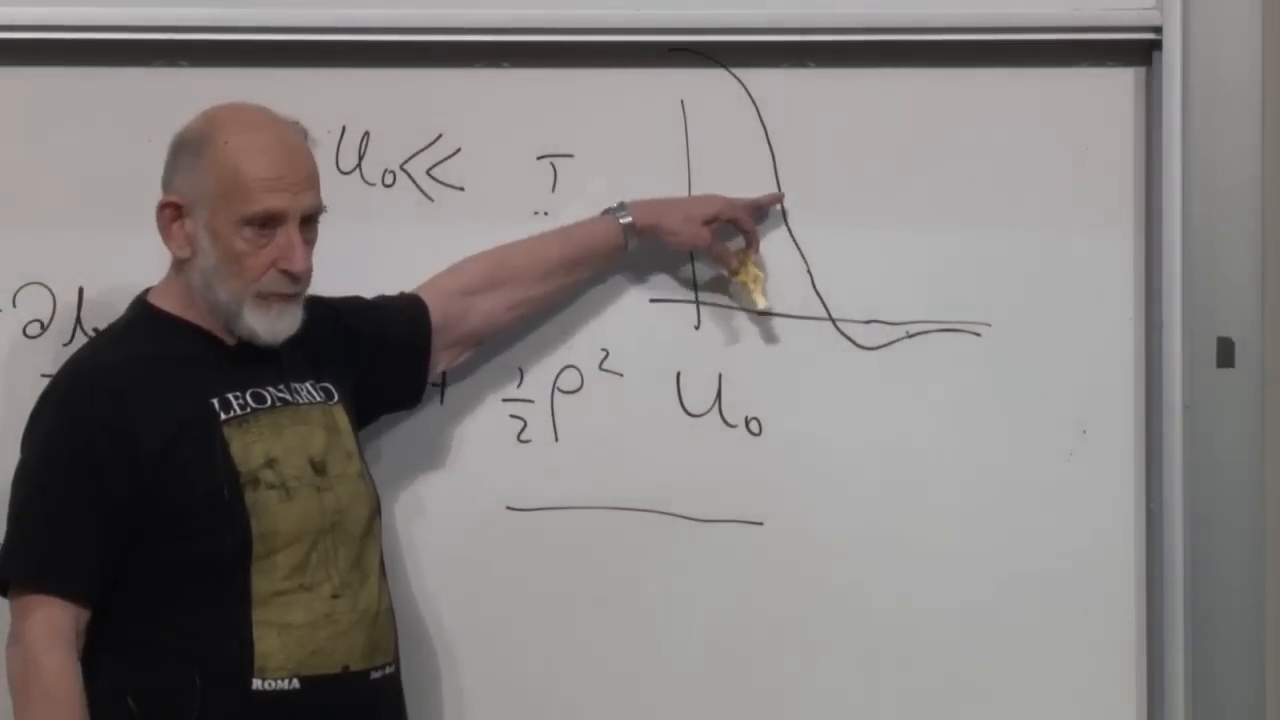
\includegraphics[width=0.90\textwidth]{lecture_06_figure_10.png}
\caption{定性的排斥和吸引对势曲线，旁边是压强公式，其修正跟随\(U_0\)的符号。}
\lectureframe{01:21:30}
\end{figure}

\begin{classroomqa}
\audiencequestion{静电斥力、引力或真实的分子力能否被纳入这一计算？}
\lecturerresponse{微观势来自原子物理、分子物理或量子物理的输入。中性分子通常表现出陡峭的短程排斥核心和较长的吸引性范德瓦尔斯尾部，常以12--6势示意性地表示。对于这样的硬核，应使用完整的Mayer函数公式。引力则不同：它是长程的，其空间积分不以所需的方式收敛，此处所用的通常短程热力学极限失效。
\lecturetimestamp{01:20:40--01:23:03}}
\end{classroomqa}

这一计算体现了一种有用的分工。微观物理提供\(u(r)\)。统计力学将该能量转化为\(Z\)，\(Z\)的导数给出宏观可观测量，而物理推理则检验其符号、密度标度、广延性和适用范围。只有在正确的能量和近似被选定之后，形式操作才是机械性的。

\section{恰当微分与路径依赖性}

现在我们更换数学语言。在\emph{恰当微分}这一说法中，恰当并不意味着数值上精确。它指的是一个一次形式是某个真正的标量函数的微分。

设\(f(x,y)\)为某片地形中某点上方的高度。一个微小位移使其改变
\begin{equation}
 df=
 \frac{\partial f}{\partial x}\,dx+
 \frac{\partial f}{\partial y}\,dy
 =f_x\,dx+f_y\,dy.
 \label{eq:sm6-total-differential}
\end{equation}
假设我们只是被给定了
\begin{equation}
 \omega=F_x(x,y)\,dx+F_y(x,y)\,dy.
 \label{eq:sm6-one-form}
\end{equation}
是否存在一个标量\(f\)满足\(\omega=df\)？混合偏导的相等要求
\begin{equation}
 \frac{\partial F_y}{\partial x}
 =
 \frac{\partial F_x}{\partial y}.
 \label{eq:sm6-exactness-condition}
\end{equation}
在单连通区域上，这个零旋度条件也是充分的。分量\((F_x,F_y)\)于是构成\(f\)的梯度。

\begin{figure}[t]
\centering
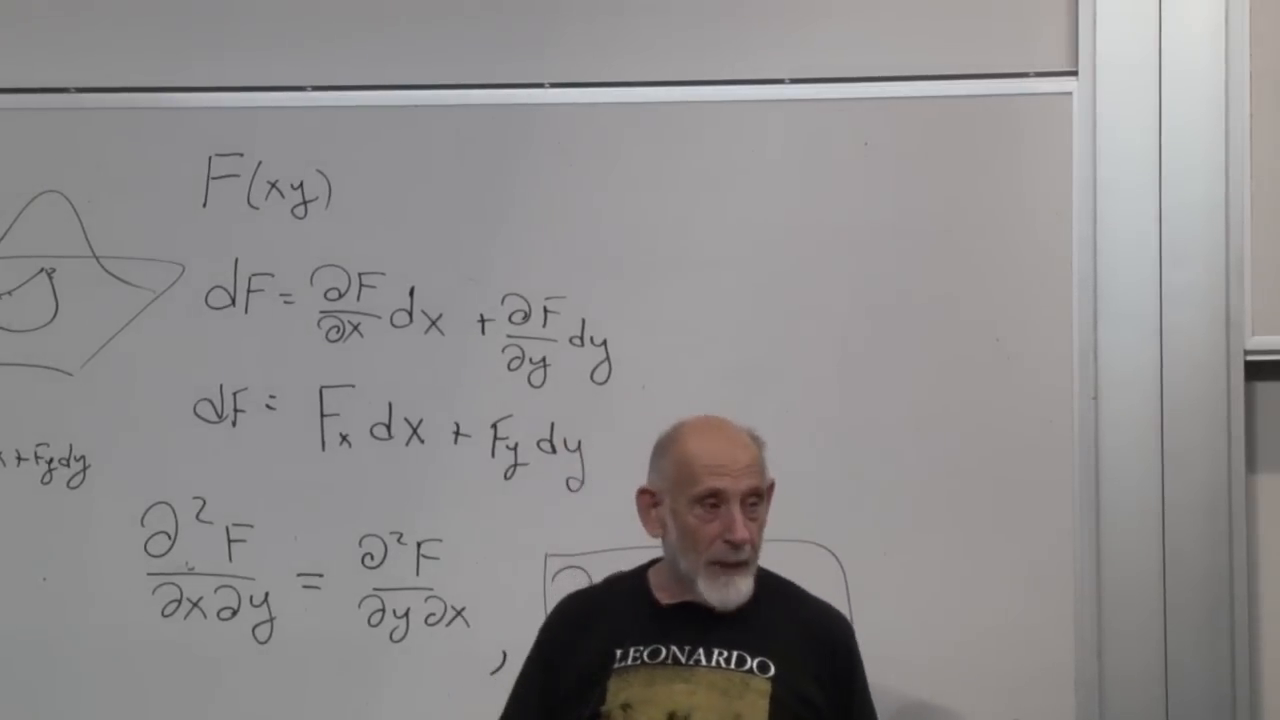
\includegraphics[width=0.90\textwidth]{lecture_06_figure_11.png}
\caption{高度作为标量函数、其微分，以及恰当性的混合偏导条件。}
\lectureframe{01:34:30}
\end{figure}

同一条件还有积分含义。若\(\omega=df\)，则
\begin{equation}
 \int_{\gamma:1\to2}\omega=f(2)-f(1)
 \label{eq:sm6-path-independent-integral}
\end{equation}
仅依赖于端点，而不依赖于路径\(\gamma\)。特别地，
\begin{equation}
 \oint_\gamma\omega=0
 \label{eq:sm6-closed-loop-zero}
\end{equation}
对每一条可收缩的闭合回路成立。

高度具有这一性质。沿平坦道路或翻越山丘在同两点之间行驶，高度的净变化相同。燃料消耗则不然。多山路线与平坦路线通常消耗不同的量，而一次闭合行程并不会恢复已燃烧的燃料。在扩展的状态描述中，剩余燃料量当然是一个定义明确的量，但它不是汽车位置\((x,y)\)单独的函数；它携带着路线的记忆。疲劳提供了同类的类比：下坡一般并不能消除上坡带来的疲劳。

\begin{classroomqa}
\audiencequestion{恰当性与保守力是同一概念吗？它与曲率有关吗？}
\lecturerresponse{旋度为零的力场是局部保守的，并允许存在势，因此这一语言密切相关。平行移动和曲率也将闭合回路的变化与局部几何数据联系起来，但那是一个更广泛的课题。这里只需要初等的陈述：零旋度意味着局部路径无关性，并带有通常关于区域的整体条件。
\lecturetimestamp{01:39:22--01:41:07}}
\end{classroomqa}

两个例子使这一检验具体化。首先取
\begin{equation}
 F_x=y,\qquad F_y=x.
 \label{eq:sm6-exact-example}
\end{equation}
两个交叉导数都等于\(1\)，确实
\begin{equation}
 \omega=y\,dx+x\,dy=d(xy).
 \label{eq:sm6-exact-example-potential}
\end{equation}
现在改变一个符号：
\begin{equation}
 F_x=y,\qquad F_y=-x.
 \label{eq:sm6-inexact-example}
\end{equation}
于是
\begin{equation}
 \frac{\partial F_x}{\partial y}=1,
 \qquad
 \frac{\partial F_y}{\partial x}=-1,
 \label{eq:sm6-inexact-cross-derivatives}
\end{equation}
因此不存在标量\(f(x,y)\)以这两个分量作为其梯度。

\begin{figure}[t]
\centering
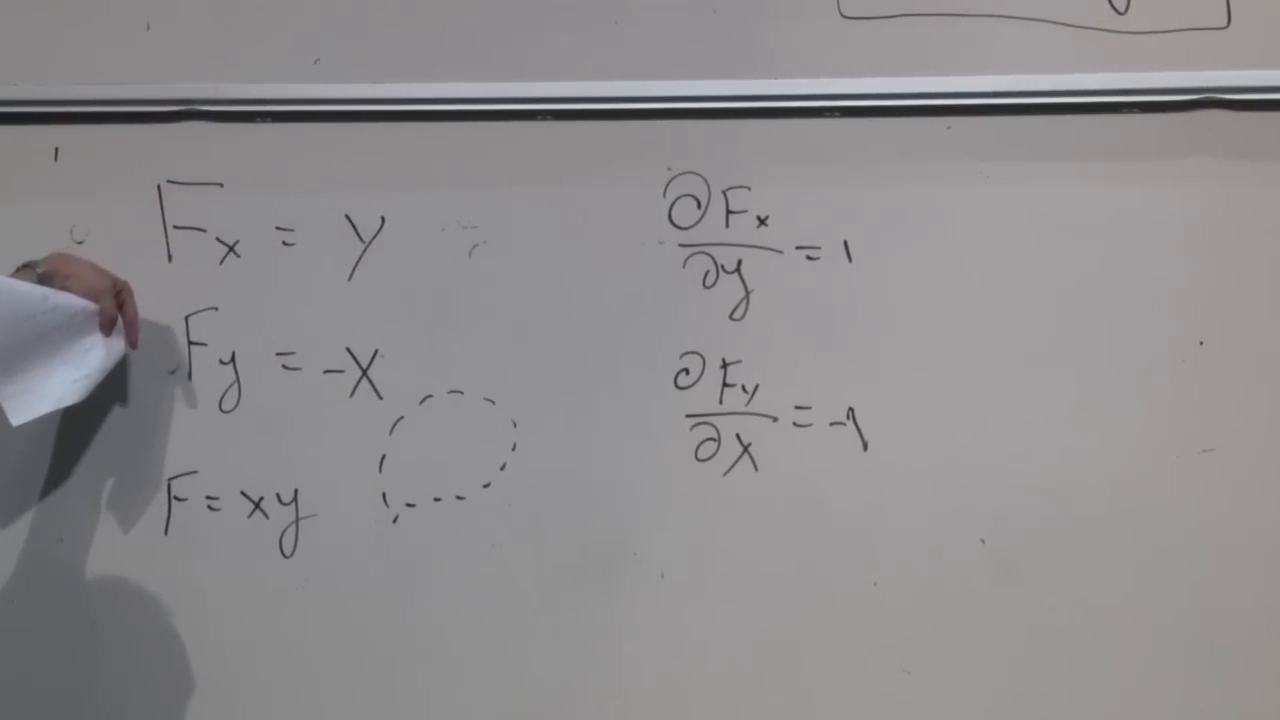
\includegraphics[width=0.90\textwidth]{lecture_06_figure_12.png}
\caption{一个由\(f=xy\)生成的恰当例子，以及一个交叉导数为\(1\)和\(-1\)的非恰当例子。}
\lectureframe{01:44:50}
\end{figure}

\section{热量与功不是态函数}

对于粒子数固定的简单可压缩系统，两个独立的平衡变量决定状态。我们可以使用\((T,V)\)、\((E,V)\)，或者，尤其对于基本关系而言自然地使用\((S,V)\)。因此
\begin{equation}
 E=E(S,V),
 \end{equation}
其恰当微分为
\begin{equation}
 dE=
 \left(\frac{\partial E}{\partial S}\right)_V dS+
 \left(\frac{\partial E}{\partial V}\right)_S dV
 =T\,dS-P\,dV.
 \label{eq:sm6-fundamental-relation}
\end{equation}

\begin{classroomqa}
\audiencequestion{绝热是指缓慢、绝热绝缘、可逆，还是等熵？}
\lecturerresponse{这一术语在不同语境中用法不同。对于此处考虑的平衡路径，变化是准静态且热绝缘的，因此是可逆且等熵的。仅仅绝缘的不可逆过程仍可产生熵，而量子绝热定理则强调参数的缓慢变化。
\lecturetimestamp{01:47:13--01:47:54}}
\end{classroomqa}

在熵固定时，膨胀使气体能量变化
\(-P\,dV\)。在体积固定时，可逆传热使其变化
\(T\,dS\)。因此，将下式写出是有用的：
\begin{equation}
 \begin{aligned}
 \delta W_{\mathrm{on}}&=-P\,dV,
 &\delta Q_{\mathrm{rev}}&=T\,dS,\\
 dE&=\delta Q_{\mathrm{rev}}+\delta W_{\mathrm{on}}.&&
 \end{aligned}
 \label{eq:sm6-first-law-increments}
\end{equation}
符号\(\delta\)而非\(d\)，预示着热和功是路径增量，而不是状态函数的微分。

\begin{figure}[t]
\centering
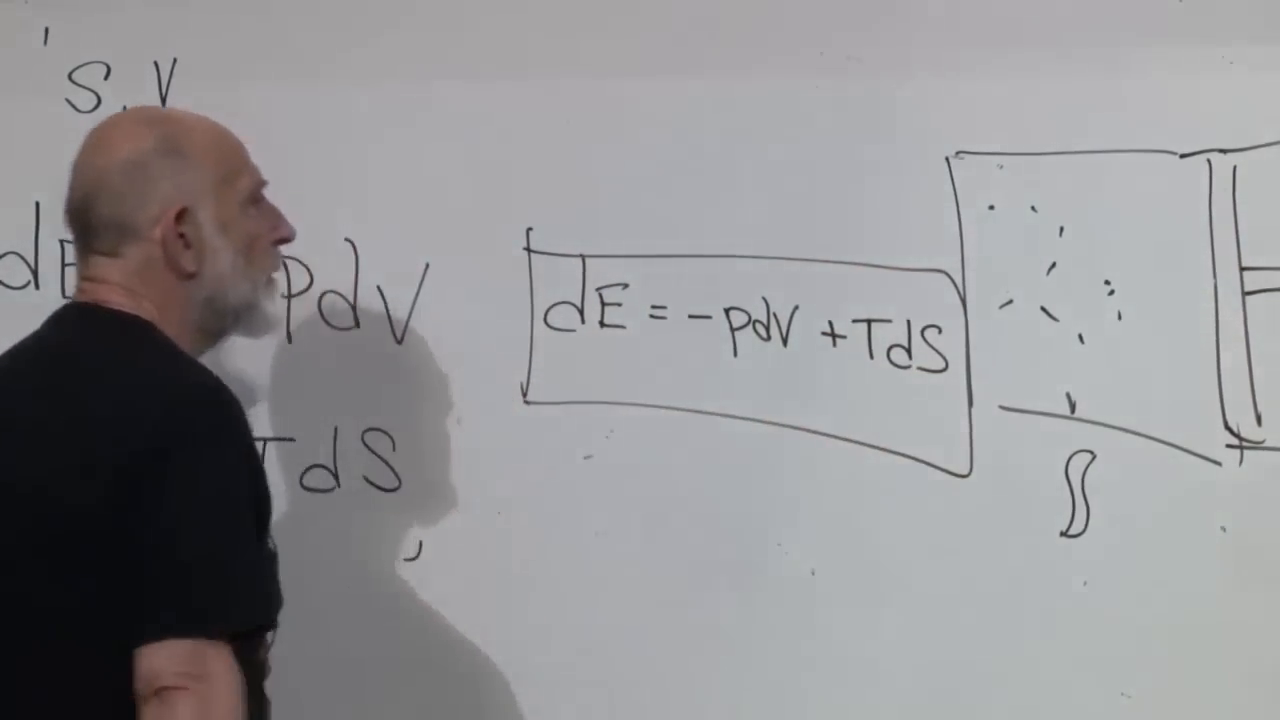
\includegraphics[width=0.90\textwidth]{lecture_06_figure_13.png}
\caption{活塞系统的第一定律：
\(dE=-P\,dV+T\,dS\)。}
\lectureframe{01:50:28}
\end{figure}

\begin{classroomqa}
\audiencequestion{\(-P\,dV\)表示对气体做的功还是气体做的功？}
\lecturerresponse{按照
\eqref{eq:sm6-first-law-increments}中的约定，它是对气体做的功。在膨胀过程中\(dV>0\)，气体对活塞做正功，因此对气体做的功为负，气体失去能量。这两种描述大小相等、方向相反。
\lecturetimestamp{01:51:23--01:52:27}}
\end{classroomqa}

等式\(\delta Q_{\mathrm{rev}}=T\,dS\)绝不能原封不动地推广到任意不可逆加热。一般而言，
\begin{equation}
 dS=\frac{\delta Q}{T_{\mathrm{boundary}}}+dS_{\mathrm{prod}},
 \qquad dS_{\mathrm{prod}}\ge 0.
 \label{eq:sm6-entropy-production}
\end{equation}
下面关于全微分的论证针对准静态平衡路径，对于这些路径，可逆关系是恰当的关系。

\begin{classroomqa}
\audiencequestion{在态空间论证中，是否假定所有路径都经过平衡态？}
\lecturerresponse{是的。这些操作进行得足够缓慢，使得\(P\)、\(T\)、\(E\)、\(S\)和\(V\)沿路径始终保持良好定义。热和功的路径依赖性并不要求系统被驱离平衡态很远。
\lecturetimestamp{01:54:30--01:54:39}}
\end{classroomqa}

要检验热是否为全微分，以\((E,V)\)为坐标并重新整理第一定律：
\begin{equation}
 \delta Q_{\mathrm{rev}}=dE+P(E,V)\,dV.
 \label{eq:sm6-heat-one-form}
\end{equation}
如果存在状态函数\(Q(E,V)\)满足\(dQ=\delta Q_{\mathrm{rev}}\)，则其偏导数必须为
\begin{equation}
 \left(\frac{\partial Q}{\partial E}\right)_V=1,
 \qquad
 \left(\frac{\partial Q}{\partial V}\right)_E=P.
 \label{eq:sm6-hypothetical-heat-derivatives}
\end{equation}
于是混合导数相等将要求
\begin{equation}
 \begin{aligned}
 \frac{\partial}{\partial V}
 \left(\frac{\partial Q}{\partial E}\right)_V
 &=\frac{\partial}{\partial E}
 \left(\frac{\partial Q}{\partial V}\right)_E,\\
 0&=\left(\frac{\partial P}{\partial E}\right)_V.
 \end{aligned}
 \label{eq:sm6-heat-exactness-requirement}
\end{equation}

\begin{classroomqa}
\audiencequestion{这与用于\(F_x\,dx+F_y\,dy\)的旋度检验完全相同吗？}
\lecturerresponse{是的。\(dE\)和\(dV\)的系数分别是\(1\)和
\(P(E,V)\)。它们的交叉导数分别是\(0\)和
\((\partial P/\partial E)_V\)。只有当这些导数一致时，热才是全微分。
\lecturetimestamp{01:54:39--01:54:52}}
\end{classroomqa}

\begin{figure}[t]
\centering
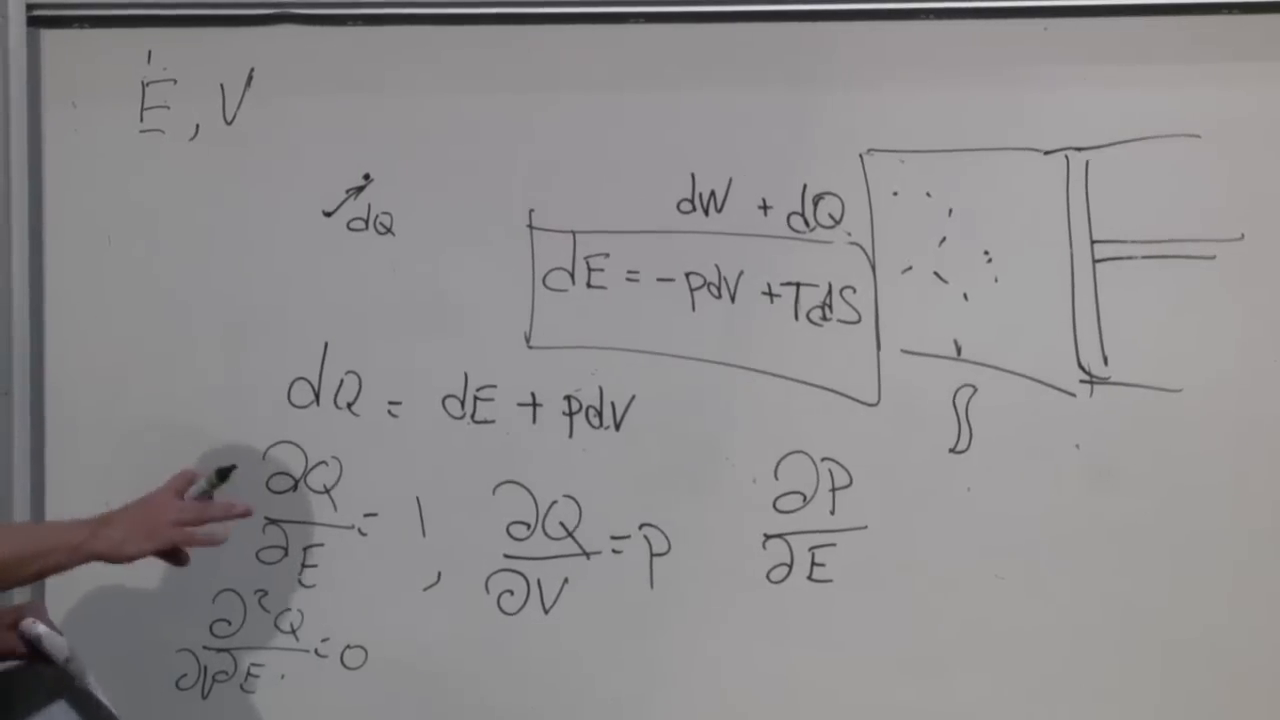
\includegraphics[width=0.90\textwidth]{lecture_06_figure_14.png}
\caption{热的一形式\(dE+P\,dV\)，以及若它是某个状态函数的微分则所需的混合导数。}
\lectureframe{01:58:10}
\end{figure}

这一要求从物理上就已经不可信：在体积固定时向气体添加能量通常会改变其压强。理想气体提供了一个直接的计算：
\begin{equation}
 PV=NT,
 \qquad
 E=\frac{3}{2}NT
 \quad\Longrightarrow\quad
 P=\frac{2E}{3V}.
 \label{eq:sm6-ideal-pressure-energy}
\end{equation}
因此
\begin{equation}
 \left(\frac{\partial P}{\partial E}\right)_V
 =\frac{2}{3V}\ne0.
 \label{eq:sm6-heat-curl-fails}
\end{equation}
旋度检验失败：\(\delta Q_{\mathrm{rev}}\)不是全微分。功的增量\(\delta W_{\mathrm{on}}=-P\,dV\)出于同样的原因也失败。

\begin{figure}[t]
\centering
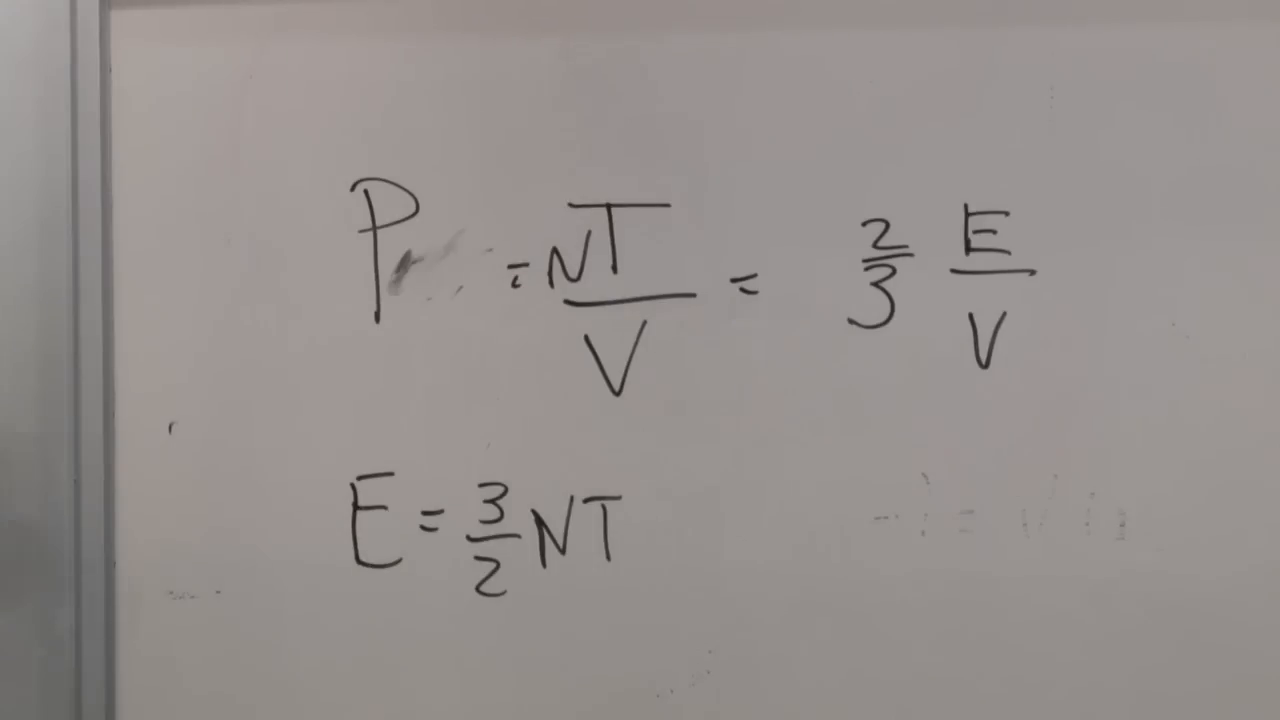
\includegraphics[width=0.90\textwidth]{lecture_06_figure_15.png}
\caption{将理想气体关系合并为
\(P=2E/(3V)\)。}
\lectureframe{02:00:00}
\end{figure}

\begin{figure}[H]
\centering
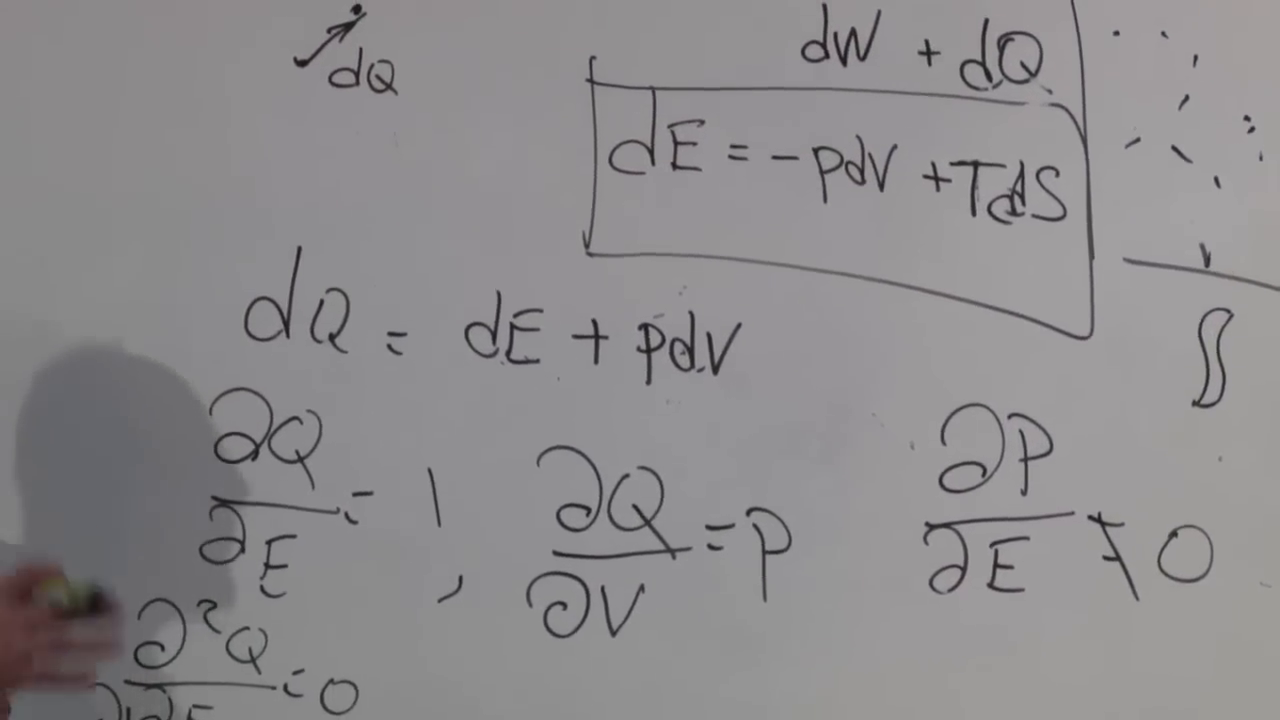
\includegraphics[width=0.90\textwidth]{lecture_06_figure_16.png}
\caption{完整的论证：因为
\((\partial P/\partial E)_V\ne0\)，热的一形式不可能是全微分。}
\lectureframe{02:00:35}
\end{figure}

对于封闭的平衡循环，
\begin{equation}
 \oint dE=0,
 \qquad
 \oint\delta Q_{\mathrm{rev}}
 =-\oint\delta W_{\mathrm{on}}.
 \label{eq:sm6-cycle-balance}
\end{equation}
系统回到相同的能量，但热和功不必分别消失。它们的值取决于在态空间中所走的路径。这就是为什么循环热机能够吸收热并输出净功，即使其工作物质回到初始热力学状态。

\begin{classroomqa}
\audiencequestion{这种路径依赖性与热机效率、滞后和记忆有关吗？}
\lecturerresponse{热机循环直接利用它：循环的热输入与净功输出相平衡，而状态函数\(E\)回到其初始值。滞后和记忆也涉及路径依赖性，尽管它们通常需要额外的内部变量或非平衡物理。目前的结论更为狭窄，并且已经对可逆平衡路径成立：热和功是转移量，而不是储存在热力学状态中的属性。
\lecturetimestamp{02:02:21--02:03:17}}
\end{classroomqa}

论证的两个部分现在汇合了。只有当其控制条件和平衡条件被指定后，测量才有意义。只有当其小参数和失效判据被指定后，近似才有意义。只有当其微分通过路径无关性检验后，热力学量才是状态函数。在每一种情形中，严谨的数学并不取代物理解释；它确切地告诉我们这种解释在何处是合理的。
\chapter{声音、量子振子与第二定律}

\lectureoverview{第二定律是最终目标，但有两个具体计算为其铺路。声速检验热力学导数如何变成可观测的运动。谐振子随后揭示经典能量均分在刚性自由度上的失效，并展示量子力学如何逐个激活模式。我们最后回到可逆微观动力学与熵增之间的表面冲突，利用相空间流、粗粒化、混沌和回归，把第二定律表述为一条压倒性地可能的定律，而不是一条毫无例外的力学禁令。}

\section{关于第二定律的一个承诺}

核心问题容易陈述，却难以解释。牛顿方程是可逆的：如果某个微观历史被允许，那么时间反演的历史也被允许。然而第二定律说宏观过程有一个优选方向，其特征是熵通常增加。我们会谈到这一张力，但不是立刻。最好先看到统计力学产生具体信息，然后在一个初等计算中遇到那个迫使经典物理让位于量子物理的历史谜题。

第一个例子是数值性的，而且刻意粗糙：估计稀薄气体中的声速。第二个在其假设范围内是精确的：计算热浴中谐振子的平均能量。振子将引导我们从能量均分走向量子化能级，从一个模式走向无穷多个模式，最后回到多粒子系统忘记其初始状态意味着什么这一问题。

\section{声速的分子尺度}

想象稀薄气体中有一个小的过密区域。它之所以扩散，是因为分子离开拥挤区域，所以其传播速度应与分子速度相当。能量均分给出一个分子的动能，
\begin{equation}
 \frac{3}{2}k_B T
 =\frac{1}{2}m\expect{v^2},
 \qquad
 \expect{v^2}=\frac{3k_B T}{m}.
 \label{eq:sm7-molecular-speed}
\end{equation}
这里温度从绝对零度起量，并且由于我们想要实验室单位，\(k_B\) 已被恢复。这个论证只是一个尺度估计：分子的均方根速度本身并不是集体声波的速度。

更系统的推导考虑一小块气体。相对两面上的压力不等会施加一个净力，而其加速度与质量密度成反比。结果具有如下形式
\begin{equation}
 c_s^2=
 \left(\frac{\partial P}{\partial \rho_m}\right)_{\cal C},
 \qquad
 \rho_m=m\rho,
 \label{eq:sm7-sound-general}
\end{equation}
其中 \(\rho\) 是数密度，下标 \({\cal C}\) 指明扰动所遵循的热力学条件。板书计算使用
\begin{equation}
 P=\rho k_B T
 \quad\Longrightarrow\quad
 \frac{1}{m}
 \left(\frac{\partial P}{\partial\rho}\right)_T
 =\frac{k_B T}{m}.
 \label{eq:sm7-sound-isothermal}
\end{equation}
这是等温声速估计。它与 \eqref{eq:sm7-molecular-speed} 相差一个因子 \(3\)（在速度平方中），或者说在速度中相差 \(\sqrt{3}\)。

\begin{figure}[t]
\centering
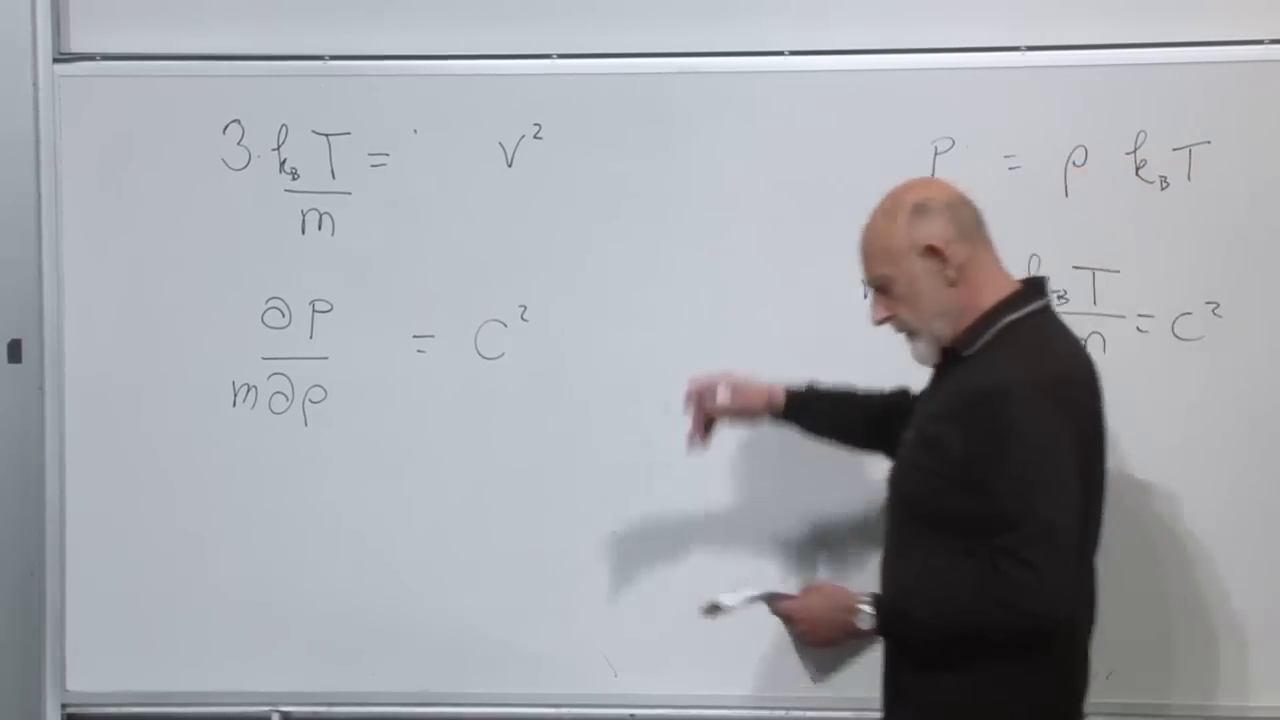
\includegraphics[width=0.90\textwidth]{lecture_07_figure_02.png}
\caption{分子速度估计、压力导数以及理想气体代换一起展示。}
\lectureframe{00:08:55}
\end{figure}

有一个重要的修正。小振幅声波压缩和稀疏气体的速度通常快于热量在相邻气体元之间流动的速度。因此局部运动近似为绝热的，而不是等温的：
\begin{equation}
 c_s^2=
 \left(\frac{\partial P}{\partial\rho_m}\right)_S.
 \label{eq:sm7-sound-adiabatic}
\end{equation}
对于绝热指数为 \(\gamma\) 的理想气体，
\begin{equation}
 P\rho_m^{-\gamma}=\text{constant},
 \qquad
 c_s^2=\gamma\frac{P}{\rho_m}
       =\gamma\frac{k_B T}{m}.
 \label{eq:sm7-sound-ideal-adiabatic}
\end{equation}
对于室温下的双原子空气，\(\gamma\simeq 7/5\)。因此，固定温度的计算是有用的初步估计，而绝热导数提供了物理上恰当的修正。

使用粗略值
\begin{equation}
\begin{aligned}
 k_B&\simeq1.3\times10^{-23}\ {\rm J\,K^{-1}},
 &T&\simeq300\ {\rm K},\\
 m_{\rm air}&\simeq4\times10^{-26}\ {\rm kg}.&&
\end{aligned}
 \label{eq:sm7-air-data}
\end{equation}
分子估计约为 \(500\ {\rm m\,s^{-1}}\)。这里的温度必须是开尔文绝对温度，而不是像华氏度那样的偏移标度。熟悉的声速约为 \(300\ {\rm m\,s^{-1}}\)，而绝热理想气体公式在室温下给出约 \(340\ {\rm m\,s^{-1}}\)。因此，粗略计算找到了正确的物理尺度。

\begin{figure}[t]
\centering
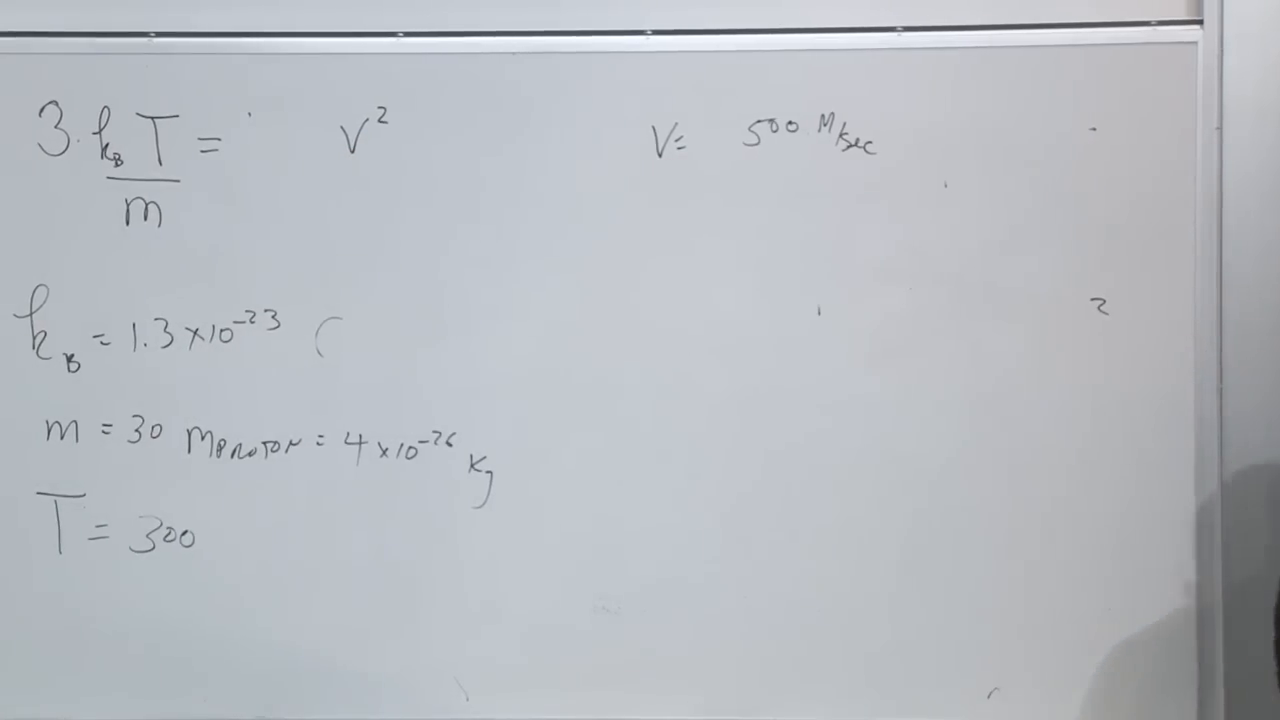
\includegraphics[width=0.90\textwidth]{lecture_07_figure_03.png}
\caption{使用玻尔兹曼常数、接近 \(30\) 个质子质量的有效分子质量以及 \(T\simeq300\ {\rm K}\) 对室温空气所作的估计。}
\lectureframe{00:10:55}
\end{figure}

早在有微观解释可用之前，人们就可以通过测量压力随密度的变化来确定声速。统计论证补充了一个引人注目的解释：由此得到的宏观速度由单个分子的热速度决定。

\begin{classroomqa}
\audiencequestion{分子质量中是否应当计入中子，而氮的数值\(14\)是否只计质子？}
\lecturerresponse{所引用的原子量已经计入了质子和中子。分子氮含有两个原子，其原子量约为\(14\)，因此其质量约为\(28\)个质子质量；对于这一估算，将\(28\)取整为\(30\)已经足够。
\lecturetimestamp{00:10:58--00:11:16}}
\end{classroomqa}

\begin{classroomqa}
\audiencequestion{因子\(3\)来自三个平动方向，而声波沿一个方向传播。这是否应当去掉因子\(3\)？}
\lecturerresponse{它正确地提醒我们，不应把三维的分子均方根速率与一维的传播速率等同起来。开头的论证只是一个数量级图像。一个受控的答案来自压强导数，并结合适用于该波的热力学条件。
\lecturetimestamp{00:11:12--00:12:00}}
\end{classroomqa}

\begin{classroomqa}
\audiencequestion{该导数是否假定了波传播过程中温度保持不变？}
\lecturerresponse{所展示的理想气体代换确实如此。对于极小的扰动，固定温度是一个合理的临时估计；标准的改进是，普通声波近似为绝热的，这会把等温导数替换为\(\left(\partial P/\partial\rho_m\right)_S\)。
\lecturetimestamp{00:12:59--00:14:01}}
\end{classroomqa}

\begin{classroomqa}
\audiencequestion{如果压强和密度的变化都很小，是否就使它们的导数很小？}
\lecturerresponse{不。导数是在无穷小极限下两个小变化量之比。\(\delta P\)和\(\delta\rho\)都可以很小，而\(\delta P/\delta\rho\)仍保持有限，并决定波速。
\lecturetimestamp{00:14:03--00:14:23}}
\end{classroomqa}

\begin{classroomqa}
\audiencequestion{当气体被压缩时，声速是否应当升高，就像从气体过渡到液体或固体时那样？}
\lecturerresponse{是的。导数是在所考虑的状态下求值的，而\(P(\rho,T)\)不必保持线性。当分子被挤压得彼此靠近时，状态方程变为非理想的，\(\partial P/\partial\rho\)可以显著增大。
\lecturetimestamp{00:14:25--00:15:13}}
\end{classroomqa}

\begin{classroomqa}
\audiencequestion{数值\(500\ {\rm m\,s^{-1}}\)能否在任意压强下使用？}
\lecturerresponse{不能。它属于低密度范围，在该范围内理想气体方程是有用的近似。一旦密度的更高次幂进入\(P(\rho,T)\)，导数、从而声速就依赖于压强和密度。
\lecturetimestamp{00:15:14--00:16:29}}
\end{classroomqa}

\begin{classroomqa}
\audiencequestion{随着密度增大，声波以大致分子速率传播的原始图像是否也会失效？}
\lecturerresponse{很可能。该图像是为稀薄气体量身定制的。在高密度下，集体相互作用变得越来越重要，这正是状态方程导数成为更一般描述的原因。
\lecturetimestamp{00:16:32--00:16:53}}
\end{classroomqa}

\begin{classroomqa}
\audiencequestion{为什么氮分子质量写成大约\(30\)个质子质量，而不是\(28\)？}
\lecturerresponse{只需要与估算相称的数值精度，因此将\(28\)取整为\(30\)。将原来的\(500\ {\rm m\,s^{-1}}\)估计值除以\(\sqrt{3}\simeq1.7\)也使其接近\(300\ {\rm m\,s^{-1}}\)，尽管绝热导数是计算修正的受控方法。
\lecturetimestamp{00:16:54--00:17:27}}
\end{classroomqa}

\section{热浴中的一个经典振子}

现在我们用一个谐振子代替自由平动的分子，并把其他一切视为热浴。弹簧上的质量块是最直接的图像，但该模型要广泛得多。电磁腔模会振荡；晶体中的原子会振荡；几乎任何稍微偏离平衡的稳定系统，在最低阶上都作简谐运动。

以\(x\)为偏离平衡的位移，动量为\(p\)，质量为\(m\)，弹簧常数为\(\kappa\)，哈密顿量为
\begin{equation}
 H(x,p)=\frac{p^2}{2m}+\frac{\kappa x^2}{2},
 \qquad
 \omega=\sqrt{\frac{\kappa}{m}}.
 \label{eq:sm7-classical-hamiltonian}
\end{equation}
热浴固定\(T\)，从这一点起我们再次使用\(k_B=1\)，因此\(\beta=1/T\)。与室温平衡的振子温度接近\(300\ {\rm K}\)；浸入液氦中的振子温度只有几开尔文。一个假想的弹簧若放在太阳中心，就不会作为弹簧存活下来，但这个例子清楚地说明了环境的作用。玻尔兹曼权重因子分解为：
\begin{equation}
 e^{-\beta H}
 =e^{-\beta p^2/(2m)}
  e^{-\beta\kappa x^2/2}.
 \label{eq:sm7-factorized-weight}
\end{equation}

\begin{figure}[t]
\centering
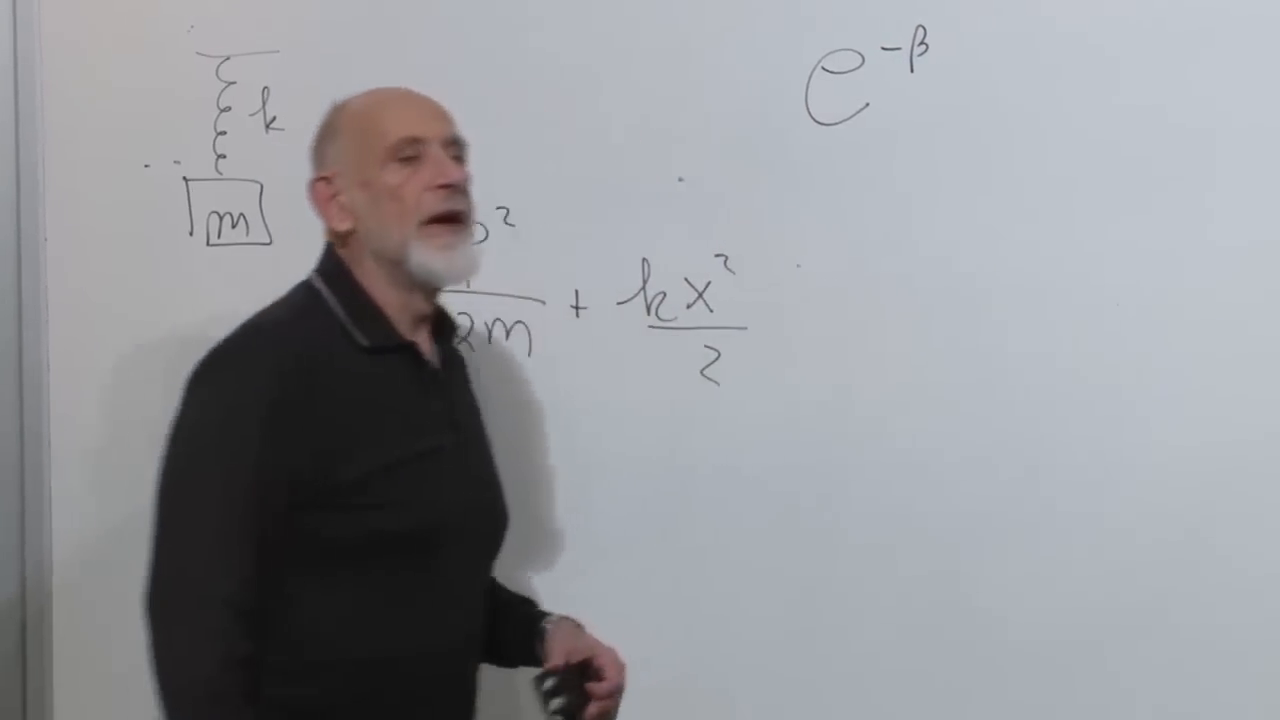
\includegraphics[width=0.90\textwidth]{lecture_07_figure_04.png}
\caption{弹簧-质量振子及其动能加势能的哈密顿量。}
\lectureframe{00:20:55}
\end{figure}

与自由气体不同，位置积分并不仅仅给出容器体积。恢复势对每个位移进行加权：
\begin{equation}
 Z_{\rm cl}
 =\frac{1}{h}\int_{-\infty}^{\infty}dp
             \int_{-\infty}^{\infty}dx\,
 e^{-\beta p^2/(2m)}
 e^{-\beta\kappa x^2/2}.
 \label{eq:sm7-classical-z}
\end{equation}
因子\(1/h\)使一维经典配分函数无量纲。它在板书计算中被略去，因为它与\(\beta\)无关，不可能影响平均能量。

\begin{figure}[t]
\centering
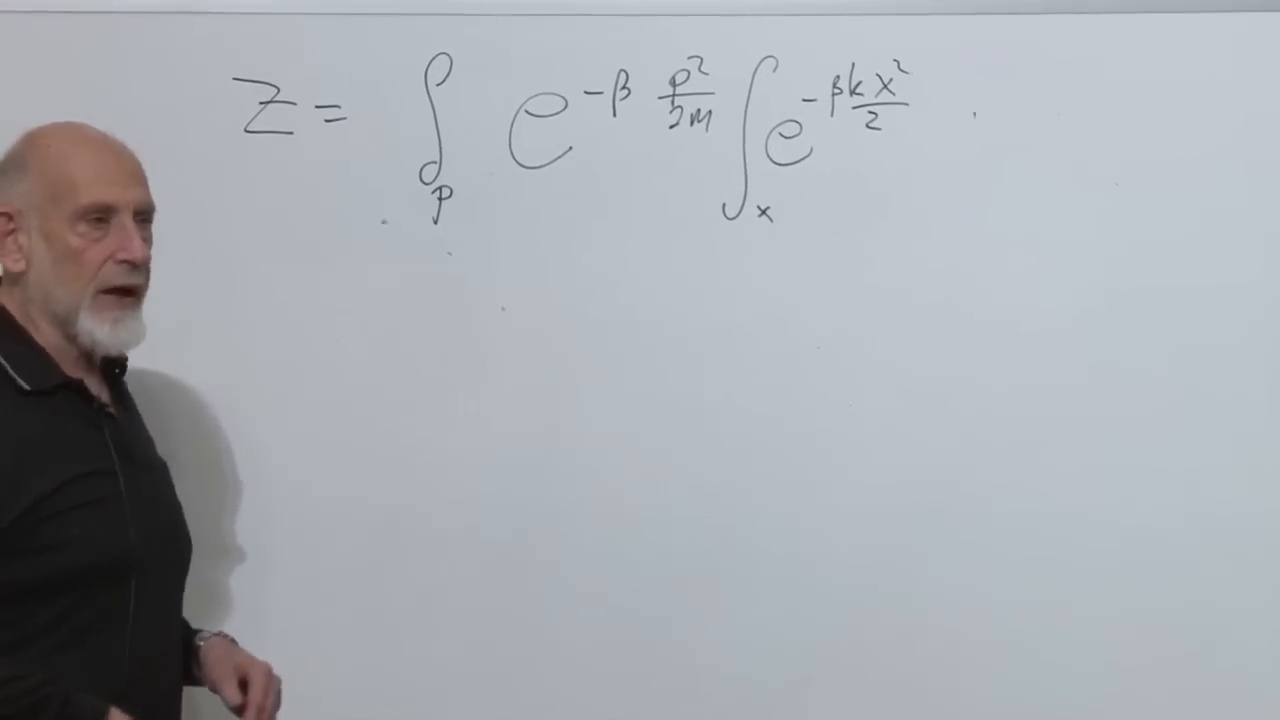
\includegraphics[width=0.90\textwidth]{lecture_07_figure_05.png}
\caption{经典振子配分函数分解为其动量与位移的高斯积分。}
\lectureframe{00:22:55}
\end{figure}

对于动量积分，令
\begin{equation}
 q=\sqrt{\frac{\beta}{2m}}\,p,
 \qquad
 dp=\sqrt{\frac{2m}{\beta}}\,dq.
 \label{eq:sm7-p-gaussian-substitution}
\end{equation}
对于位置积分，令
\begin{equation}
 y=\sqrt{\frac{\beta\kappa}{2}}\,x,
 \qquad
 dx=\sqrt{\frac{2}{\beta\kappa}}\,dy.
 \label{eq:sm7-x-gaussian-substitution}
\end{equation}
由于\(\int_{-\infty}^{\infty}e^{-u^2}\,du=\sqrt{\pi}\)，板书上所用的未归一化相空间积分为
\begin{equation}
 \int dp\,dx\,e^{-\beta H}
 =\frac{2\pi}{\beta}\sqrt{\frac{m}{\kappa}}
 =\frac{2\pi}{\beta\omega}.
 \label{eq:sm7-classical-z-unnormalized}
\end{equation}
恢复相空间元胞后，
\begin{equation}
 Z_{\rm cl}=\frac{2\pi}{h\beta\omega}
           =\frac{1}{\beta\hbar\omega}.
 \label{eq:sm7-classical-z-normalized}
\end{equation}

只有\(\beta\)依赖关系对能量有影响：
\begin{equation}
 \begin{aligned}
 \log Z_{\rm cl}&=\text{constant}-\log\beta,\\
 \expect{H}
 &=-\frac{\partial\log Z_{\rm cl}}{\partial\beta}\\
 &=\frac{1}{\beta}=T.
 \end{aligned}
 \label{eq:sm7-classical-energy}
\end{equation}

\begin{figure}[t]
\centering
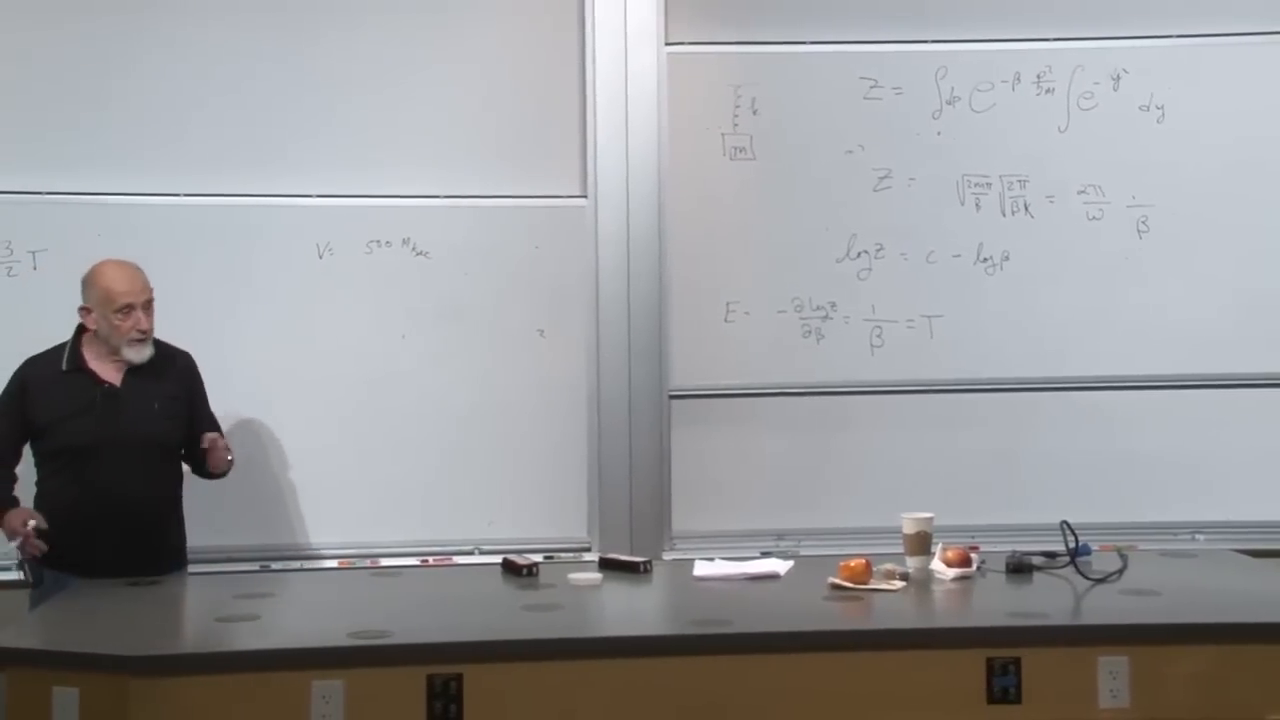
\includegraphics[width=0.90\textwidth]{lecture_07_figure_06.png}
\caption{右侧黑板上的完整经典推导链：高斯因子化、\(Z\propto(\beta\omega)^{-1}\)以及\(\expect{H}=1/\beta=T\)。}
\lectureframe{00:30:15}
\end{figure}

没有因子\(3\)，因为这是一个空间振子。也不存在剩余的因子\(1/2\)，因为有两个独立的二次项。每个高斯积分贡献\(T/2\)：
\begin{equation}
 \expect{K}=\frac{T}{2},
 \qquad
 \expect{U}=\frac{T}{2},
 \qquad
 \expect{H}=T.
 \label{eq:sm7-equipartition-oscillator}
\end{equation}
这是能量均分最实用的形式：经典哈密顿量中每一个独立的二次项都贡献\(T/2\)。

答案与\(m\)和\(\kappa\)都无关。运动本身确实依赖于这些参数：
\begin{equation}
 \expect{p^2}=mT,
 \qquad
 \expect{x^2}=\frac{T}{\kappa},
 \qquad
 \expect{\dot{x}^2}=\frac{T}{m}.
 \label{eq:sm7-classical-fluctuations}
\end{equation}
因此较重的质量运动得更慢，较硬的弹簧振幅更小，尽管平均能量仍为\(T\)。当\(\kappa\)被取得极大时，这就变得令人不安。硬得无法运动的弹簧应当看起来像冻结的约束，然而经典能量均分仍然赋予它能量\(T\)。

\begin{classroomqa}
\audiencequestion{当\(\kappa\to\infty\)时，配分函数趋于零。它的对数怎么还能使用？}
\lecturerresponse{保持\(\kappa\)有限但任意大。它对\(\log Z\)的贡献是可加的且与\(\beta\)无关，因此对\(\beta\)求导仍然给出\(T\)。这种极限下的不适感是真实的：经典计算内部自洽，但它遗漏了自然界对于极硬振子所必需的一个特征。
\lecturetimestamp{00:34:01--00:34:54}}
\end{classroomqa}

\begin{classroomqa}
\audiencequestion{理想气体配分函数需要一个\(N!\)。这里是否应有类似的阶乘？}
\lecturerresponse{没有。我们研究的是一个指定的振子，而不是对\(N\)个全同粒子进行排列。对于许多独立的标记模式，配分函数相乘。不可区分性因子属于另一个计数问题。
\lecturetimestamp{00:35:03--00:35:40}}
\end{classroomqa}

\section{为什么经典能量均分是一场危机}

真实分子并非无结构的点。双原子分子包含一个可以振动的键，因而有一个内部振子。朴素的经典计数即使在常温下也会给该模式分配额外的热能。在一个刻意简化的示意性计数中，激活一个振动振子会把\(3T/2\)的能量推向\(5T/2\)。精确的热容记账还必须包括转动自由度，并区分能量与其对温度的导数。决定性的实验事实更简单：刚性内部模式在低温下并未像经典能量均分所要求的那样作出贡献。

人们可以否认分子具有内部结构，但这是荒谬的；或者承认经典力学缺少一个要素。这个要素就是量子力学。我们只需要它极少的一部分：谐振子具有等间距的能级。

\section{量子振子}

首先移动能量原点，将激发谱写为
\begin{equation}
 E_n^{\rm exc}=n\hbar\omega,
 \qquad n=0,1,2,\ldots.
 \label{eq:sm7-shifted-spectrum}
\end{equation}
配分函数现在是一个真正的求和，而不是相空间积分：
\begin{align}
 Z_{\rm exc}
 &=\sum_{n=0}^{\infty}e^{-\beta n\hbar\omega} \notag\\
 &=1+x+x^2+\cdots
  =\frac{1}{1-x},
 \qquad x=e^{-\beta\hbar\omega}, \notag\\
 &=\frac{1}{1-e^{-\beta\hbar\omega}}.
 \label{eq:sm7-quantum-z}
\end{align}

\begin{figure}[t]
\centering
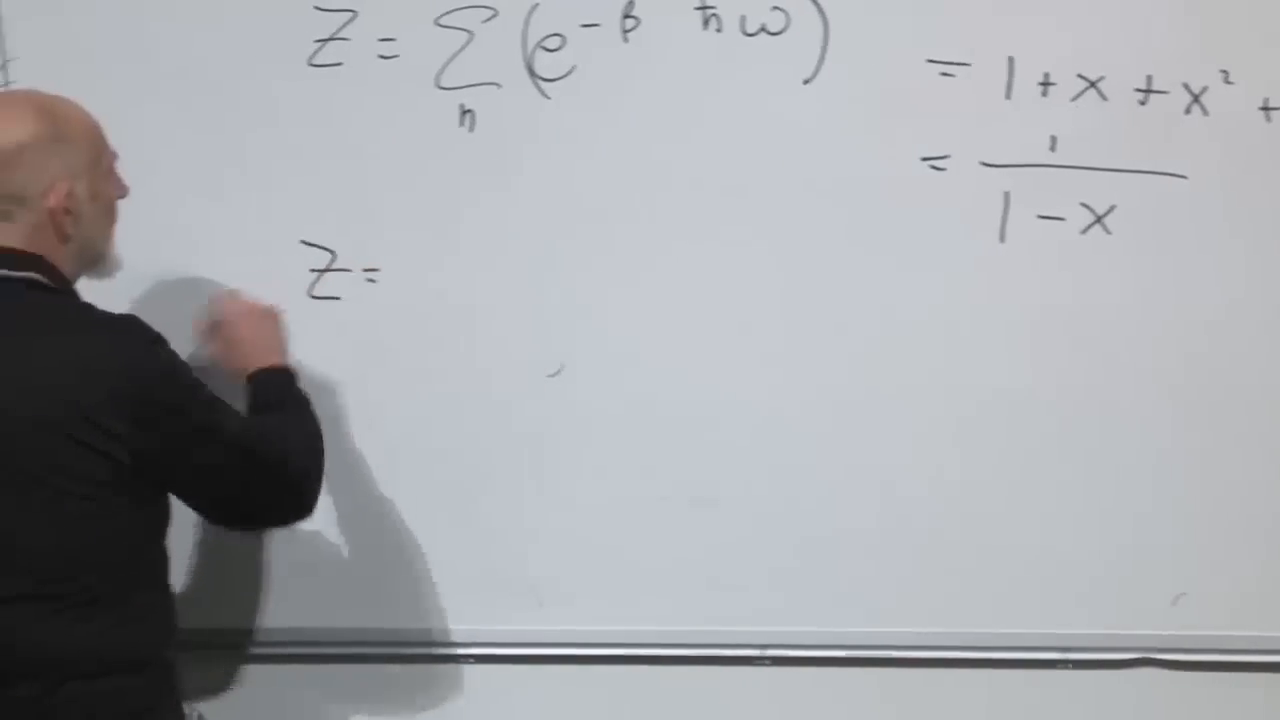
\includegraphics[width=0.90\textwidth]{lecture_07_figure_07.png}
\caption{等间距能级以及量子振子配分函数的几何级数求值。}
\lectureframe{00:42:05}
\end{figure}

求导给出平均激发能量：
\begin{align}
 E_{\rm exc}
 &=-\frac{\partial\log Z_{\rm exc}}{\partial\beta}
  =-\frac{1}{Z_{\rm exc}}
    \frac{\partial Z_{\rm exc}}{\partial\beta}
 \notag\\
 &=\hbar\omega\,
   \frac{e^{-\beta\hbar\omega}}
        {1-e^{-\beta\hbar\omega}}
  =\frac{\hbar\omega}{e^{\beta\hbar\omega}-1}.
 \label{eq:sm7-quantum-energy}
\end{align}

\begin{figure}[t]
\centering
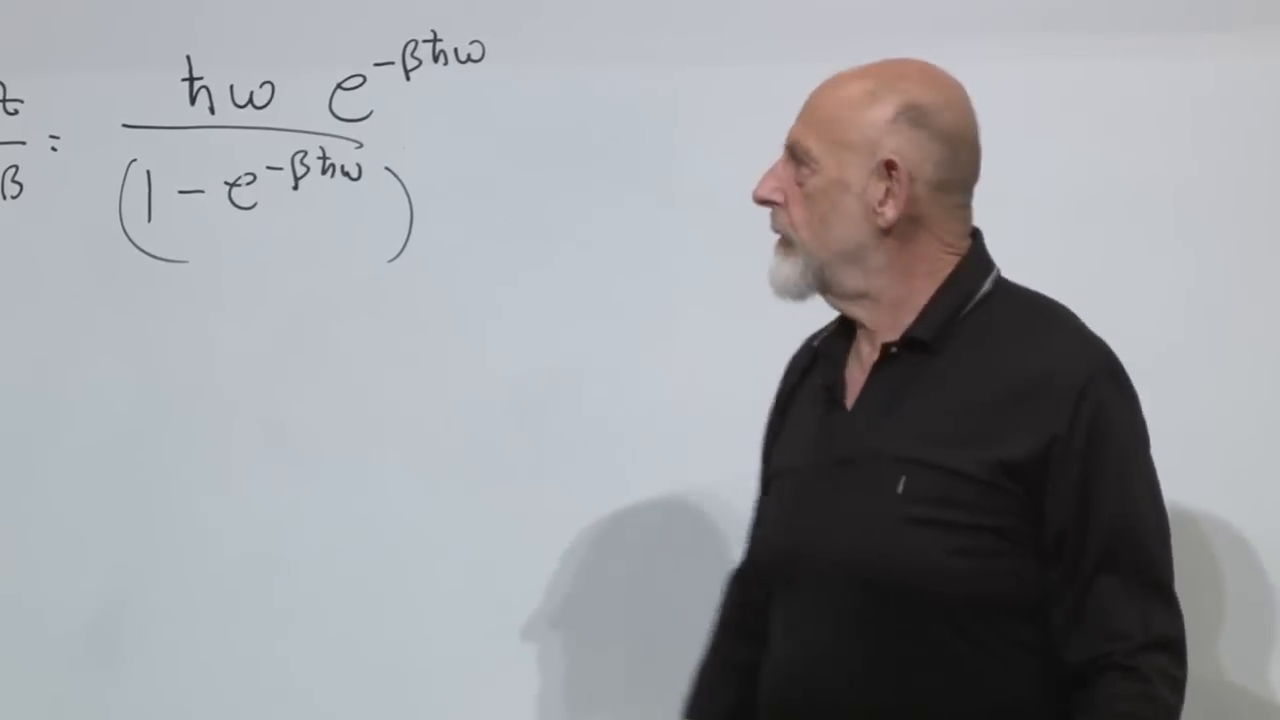
\includegraphics[width=0.90\textwidth]{lecture_07_figure_08.png}
\caption{由量子配分函数的\(\beta\)导数得到的热激发能量。}
\lectureframe{00:46:05}
\end{figure}

\subsection{高温}

当\(\beta\hbar\omega\ll1\)时，
\begin{equation}
 e^{-\beta\hbar\omega}
 =1-\beta\hbar\omega
  +O\!\left((\beta\hbar\omega)^2\right).
 \label{eq:sm7-high-t-expansion}
\end{equation}
\eqref{eq:sm7-quantum-energy}的分子趋于\(\hbar\omega\)，而分母在领头阶为\(\beta\hbar\omega\)。因此
\begin{equation}
 E_{\rm exc}\simeq\frac{1}{\beta}=T.
 \label{eq:sm7-high-t-energy}
\end{equation}
当许多能级间距都落在热能之内时，量子答案恢复经典能量均分。

\subsection{低温}

当 \(\beta\hbar\omega\gg1\) 时，指数项极小：
\begin{equation}
 E_{\rm exc}
 \simeq\hbar\omega e^{-\beta\hbar\omega}.
 \label{eq:sm7-low-t-energy}
\end{equation}
振子的热激发受到指数抑制。在平移后的约定中它几乎为零；物理上的零点能将在下文恢复。

\begin{figure}[t]
\centering
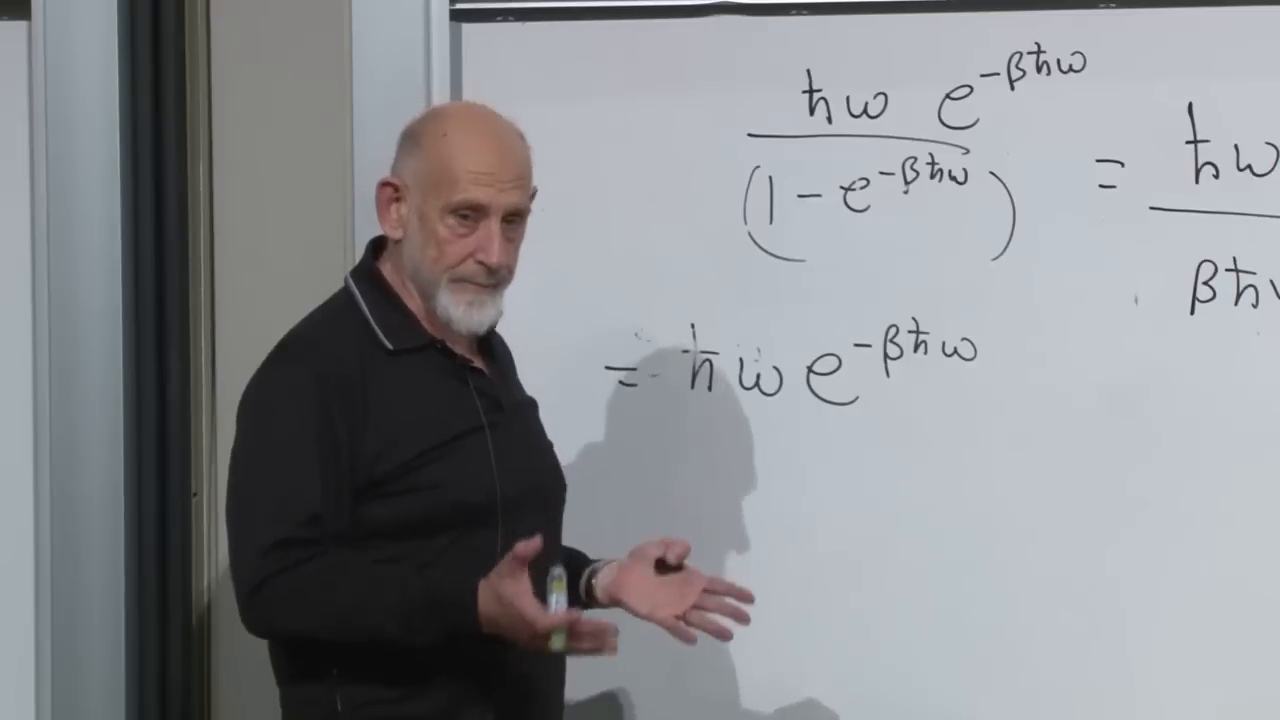
\includegraphics[width=0.90\textwidth]{lecture_07_figure_09.png}
\caption{低温展开：第一热激发受到 \(e^{-\beta\hbar\omega}\) 的抑制。}
\lectureframe{00:51:55}
\end{figure}

交叉发生在
\begin{equation}
 \beta\hbar\omega\sim1,
 \qquad\text{or equivalently}\qquad
 T\sim\hbar\omega.
 \label{eq:sm7-crossover}
\end{equation}
这一条件有直接的含义。经典能量均分给出振子能量 \(T\)。当该尺度低于一个能级间距时，量子效应便不可避免。因此
\begin{equation}
\begin{aligned}
 \hbar\omega\gg T&:\quad \text{frozen and quantum},\\
 \hbar\omega\ll T&:\quad \text{active and classical}.
\end{aligned}
 \label{eq:sm7-regimes}
\end{equation}
更硬的弹簧有更大的 \(\omega=\sqrt{\kappa/m}\)，因此需要更高的温度才能表现为经典行为。

\section{加热物质时自由度显现}

在低温下，双原子分子在热学上可以像一个点粒子，因为其刚性键振动被冻结。当 \(T\) 升高越过 \(\hbar\omega\) 时，振动模式被激活。转动模式可能在更低的尺度上激活；更高的温度会揭示更多内部运动，并最终使原子电离。加热并非仅仅向一份固定的模式清单中注入更多能量。它揭示出在较低温度下不可见的自由度。

一个假想的嵌套分子能更清楚地说明这一点。两个原子由一根刚性弹簧连接，而其中一个看似原子的部分本身又是一对由更硬弹簧连接的原子。在低 \(T\) 下，两种结构都看起来像点。在第一个阈值处，外层振动出现；在第二个阈值处，内部结构出现。系统的复杂性随着能量尺度被逐级揭示。

\begin{classroomqa}
\audiencequestion{一旦振子已处于经典区域，继续加热会使弹簧变紧还是改变其频率？}
\lecturerresponse{不会。弹簧常数和频率保持不变。更高的温度产生更大的典型动量和振幅，因而能量更大。刚度决定经典定律从哪个温度开始，而不是弹簧随温度变紧。
\lecturetimestamp{01:03:17--01:05:11}}
\end{classroomqa}

\subsection{晶体与爱因斯坦的比热}

晶体包含大量振动模式。经典能量均分给每个活跃振子分配 \(T\) 量级的能量，因此高估了低温热容。爱因斯坦的 1907 模型以量子力学方式处理晶体振动，并说明了为什么在热能未达到其能级间距之前这些振动会受到抑制。更精确的固态模型允许模式频率有一个分布，但冻结原理在爱因斯坦的计算中已经存在。

\begin{classroomqa}
\audiencequestion{这是爱因斯坦获得诺贝尔奖的工作吗？它是否只在量子力学建立之后才出现？}
\lecturerresponse{不是。诺贝尔奖的授奖说明涉及光电效应。比热模型发表于 1907，远在量子力学完整基础被理解之前。爱因斯坦接受并发展了关键的量子思想，尽管他后来反对成熟理论的某些方面。
\lecturetimestamp{00:58:38--01:03:16}}
\end{classroomqa}

\begin{classroomqa}
\audiencequestion{经典统计力学把对离散态的求和替换为对位置和动量的看似均匀的积分。是什么为这种态计数提供了依据？}
\lecturerresponse{最终的依据来自量子力学。在高温极限下，
\[
 Z_{\rm exc}\simeq\frac{1}{\beta\hbar\omega},
\]
这恰好与无量纲的经典结果 \eqref{eq:sm7-classical-z-normalized} 相符。当能级间距无法分辨时，相空间中的量子胞元就变成经典相空间测度。
\lecturetimestamp{00:59:38--01:03:06}}
\end{classroomqa}

\subsection{一根弦包含无穷多个振子}

小提琴弦或吉他弦分解为简正模式：基频、更高次谐波，以及越来越短的波长。数学上有无穷多个振子模式。如果经典能量均分给每一个模式分配能量 \(T\)，那么处于热平衡的弦将具有无穷大的能量。量子力学阻止了这种灾难。最短波长的模式具有最高频率，在任何有限温度下都保持冻结；随着 \(T\) 升高，越来越多的模式被激活。同样的逻辑后来将成为黑体辐射的基础。

\begin{figure}[t]
\centering
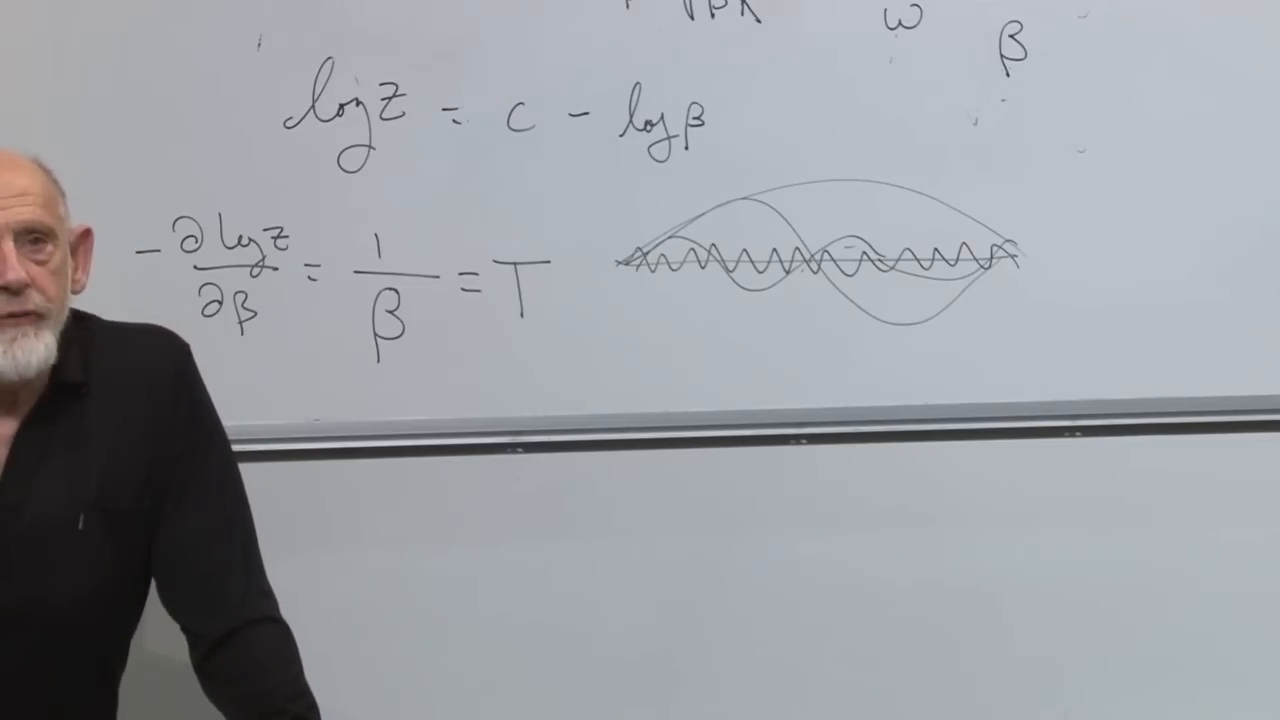
\includegraphics[width=0.90\textwidth]{lecture_07_figure_10.png}
\caption{叠加在弦上的若干简正模式，说明为什么连续弦是无穷多个谐振子的集合。}
\lectureframe{01:09:30}
\end{figure}

\begin{classroomqa}
\audiencequestion{量子到经典的过渡能否被直接观测到，加热又能否逆转低温行为？}
\lecturerresponse{能。晶体比热的温度依赖性使振动模式的冻结以及随后的激活变得可以明确测量。
\lecturetimestamp{01:09:11--01:10:13}}
\end{classroomqa}

\begin{classroomqa}
\audiencequestion{对于许多振子，我们是否对每个模式重复单振子配分函数？}
\lecturerresponse{对于独立模式，
\[
\begin{aligned}
 Z_{\rm tot}&=\prod_j Z_j,&
 \log Z_{\rm tot}&=\sum_j\log Z_j,\\
 E_{\rm tot}&=\sum_j E_j.&&
\end{aligned}
\]
满足\(\hbar\omega_j\gg T\)的模式对热贡献呈指数级小；低于该阈值的模式则有可观贡献。
\lecturetimestamp{01:10:14--01:11:00}}
\end{classroomqa}

\begin{classroomqa}
\audiencequestion{振子的零点能\(\hbar\omega/2\)怎么了？}
\lecturerresponse{物理能级为
\[
 E_n=\left(n+\frac12\right)\hbar\omega.
\]
因此
\[
 \begin{aligned}
 Z_{\rm phys}
 &=e^{-\beta\hbar\omega/2}Z_{\rm exc},\\
 E_{\rm phys}
 &=\frac{\hbar\omega}{2}
  +\frac{\hbar\omega}{e^{\beta\hbar\omega}-1}.
 \end{aligned}
\]
这一共同平移不改变能级概率、熵、热容或热激发能，但它确实使绝对平均能量平移了\(\hbar\omega/2\)。\(Z\)中的乘性因子依赖于\(\beta\)，因此当需要绝对能量时，不能将其丢弃。
\lecturetimestamp{01:11:08--01:11:37}}
\end{classroomqa}

\section{作为可逆性谜题的第二定律}

现在我们可以回到之前承诺要讨论的问题。第二定律说，普通的宏观演化是不可逆的，并且熵倾向于增加。微观的哈密顿演化是可逆的。一个对精确状态的可逆映射，如何能产生关于宏观状态的不可逆定律？

用高维相空间中的一个点来表示系统，
\[
 \Gamma=(q_1,\ldots,q_N,p_1,\ldots,p_N).
\]
我们的知识通常不是一个精确的点。假设它是紧致区域\(A\)上的均匀概率密度，其体积为\(\Omega_A\)：
\begin{equation}
 f(\Gamma)=
 \begin{cases}
  1/\Omega_A,&\Gamma\in A,\\
  0,&\Gamma\notin A.
 \end{cases}
 \label{eq:sm7-uniform-blob}
\end{equation}
在\(k_B=1\)的单位制下，其细粒化吉布斯熵为
\begin{equation}
 S_{\rm fine}
 =-\int d\Gamma\,f\log f
 =\log\Omega_A.
 \label{eq:sm7-blob-entropy}
\end{equation}
区域越小意味着信息越多、熵越低。这确定了符号：不确定性增加会扩大被占据的区域并提高\(\log\Omega_A\)。

\begin{figure}[t]
\centering
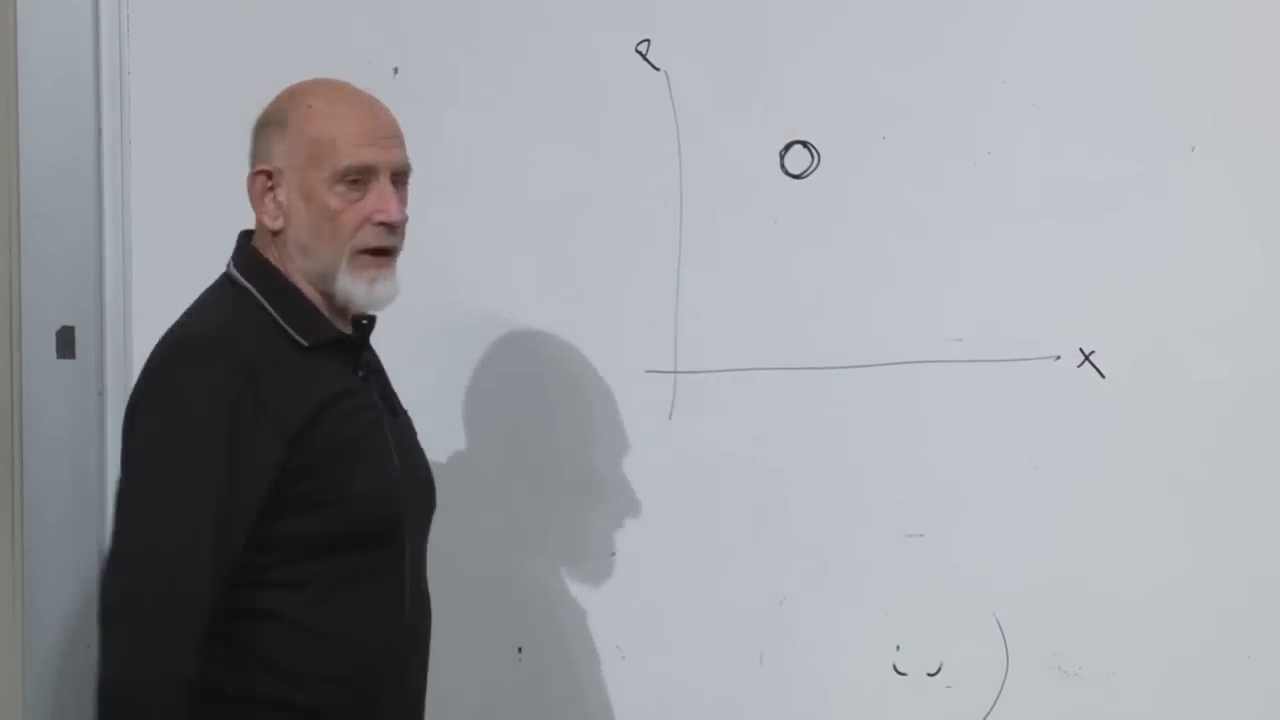
\includegraphics[width=0.90\textwidth]{lecture_07_figure_11.png}
\caption{完整位置-动量相空间的示意性二维切片中的一个紧致概率区域。}
\lectureframe{01:20:20}
\end{figure}

\begin{classroomqa}
\audiencequestion{系统是否受到物理约束而必须留在所画区域之内，它是否已经处于平衡？}
\lecturerresponse{不。该区域描述的是关于初始状态已知的信息，而不是相空间中的一堵墙。它不必是平衡分布。一个最初被限制在房间一角容器中的气体，就是特殊的非平衡信息的一个具体例子。
\lecturetimestamp{01:14:55--01:15:24}}
\end{classroomqa}

\section{刘维尔流与粗粒化增长}

刘维尔定理说，哈密顿流保持相空间体积。精确区域可以平移、拉伸、折叠并变得极其细薄，但
\begin{equation}
 \Omega_{A(t)}=\Omega_{A(0)},
 \qquad
 S_{\rm fine}(t)=S_{\rm fine}(0).
 \label{eq:sm7-liouville}
\end{equation}
其离散类比是状态的可逆置换。如果最初知道一个骰子处于两种状态之一，一对一的演化可以改变它们是哪两种状态，但不会改变可能性的数目。

真实的描述具有有限分辨率。量子力学提供了一个自然的相空间胞元，而经典实验即使不援引量子理论也具有有限的测量能力。在哈密顿流下，区域可以变成一条细长的蛇。如果相邻折叠之间的间隔低于分辨率尺度，我们就用粗粒胞元代替每个无法分辨的邻域。精确占据体积保持不变，但粗粒胞元的并集增大了：
\begin{equation}
 \Omega_{\rm coarse}(t)\geq\Omega_{A(t)},
 \qquad
 S_{\rm coarse}(t)=\log\Omega_{\rm coarse}(t).
 \label{eq:sm7-coarse-entropy}
\end{equation}

\begin{figure}[t]
\centering
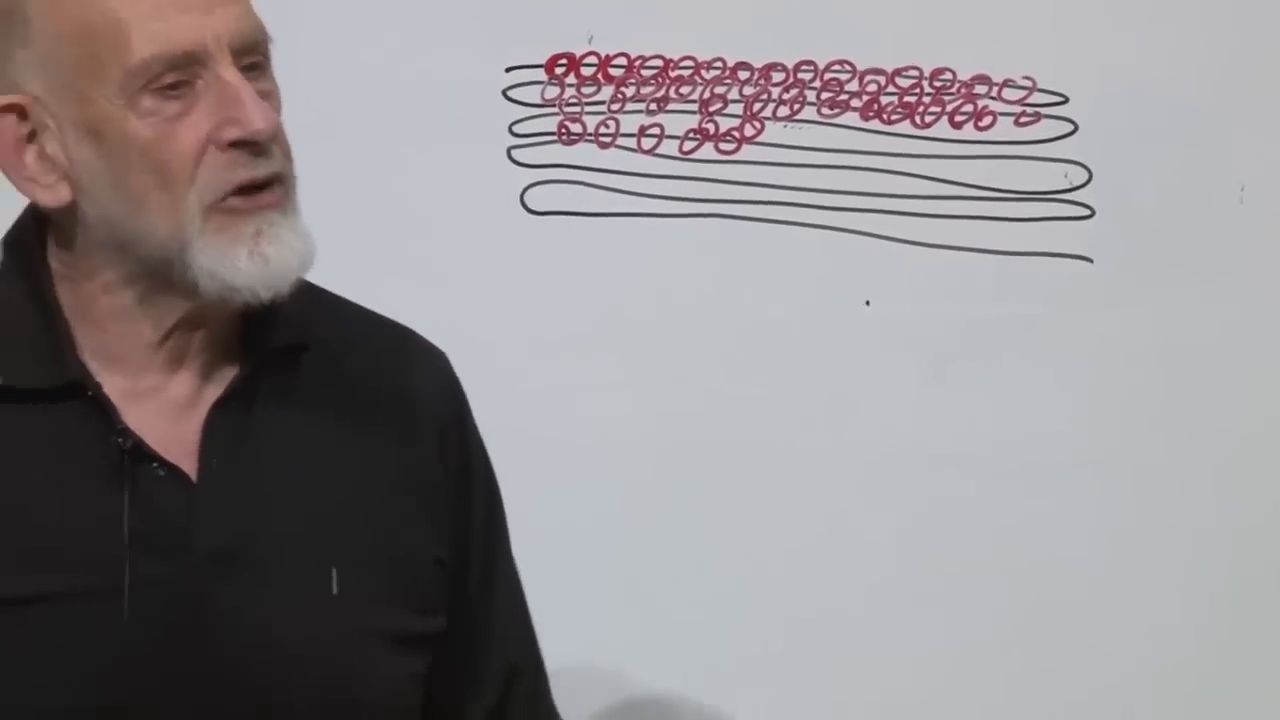
\includegraphics[width=0.90\textwidth]{lecture_07_figure_12.png}
\caption{通过有限分辨率胞元观察的保体积细丝。精确的黑色细丝保持其面积；红色粗粒胞元占据更大的有效区域。}
\lectureframe{01:22:10}
\end{figure}

\begin{classroomqa}
\audiencequestion{粗粒胞元发生重叠。这是否违反刘维尔定理？}
\lecturerresponse{不。刘维尔定理支配的是精确细丝，它保持一对一且保体积。重叠属于我们模糊的描述：我们已经丢弃了关于状态位于哪条细丝中的信息。
\lecturetimestamp{01:21:32--01:21:50}}
\end{classroomqa}

一个有用的类比是棉花。所有纤维的材料体积可以几乎保持不变，而一团被扯松的棉絮在无法分辨单根纤维的观察者看来却占据很大的表观体积。同样，相空间区域会长出越来越细的触须；那些触须又会长出更细的触须。任何固定的有限分辨率最终都无法跟上它们。

\begin{classroomqa}
\audiencequestion{熵是否只是在经典意义上看似增加，而量子力学通过施加基本的分辨率极限才使这种增加成为真实的？}
\lecturerresponse{粗粒化论证并不需要量子极限。熵同时指系统及其描述中所保留的宏观区分。在拥有无限微观信息时，细粒化熵是常数；在任何固定的有限分辨率下，混沌细丝最终变得无法分辨，粗粒化熵随之增加。
\lecturetimestamp{01:24:04--01:25:20}}
\end{classroomqa}

\section{混沌、有限的可达区域与平衡化}

对于盒中的气体，位置是有界的。在固定的有限总能量下，动量同样有界，即使全部能量暂时集中在一个粒子上也是如此。因此，在通常的约束假设下，动力学上可及的能量壳层具有有限测度。

\begin{figure}[t]
\centering
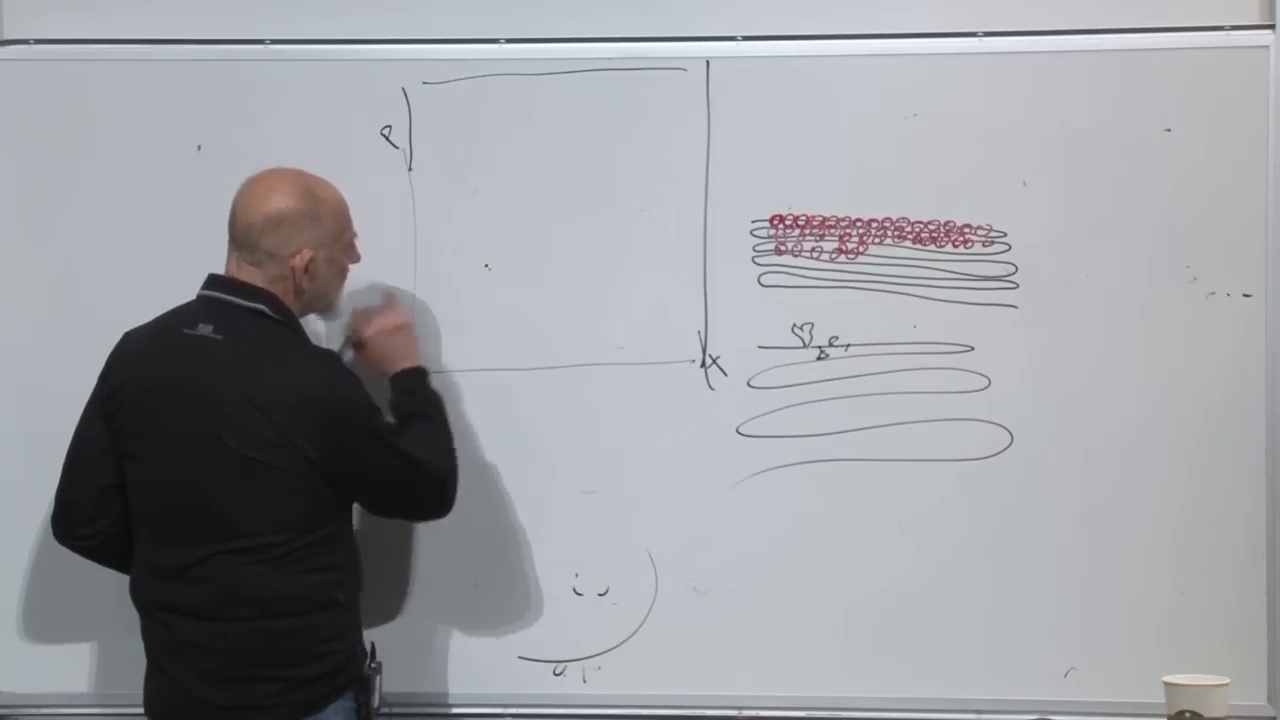
\includegraphics[width=0.90\textwidth]{lecture_07_figure_13.png}
\caption{有界的可及相空间区域，旁边是细丝及其粗粒化表示。}
\lectureframe{01:28:10}
\end{figure}

混沌系统中邻近的初始点在最初一段时间内遵循相似的历史，随后分离。在一次台球开球中，母球方向上一个不可察觉的变化会被复制到随后的碰撞中；差异不断累积，直到最终构型彼此无关。因此，整个初始斑块在可及区域中被拉伸和折叠。在有限分辨率下，它趋近于一种宽广、近乎均匀的平衡描述。

\begin{figure}[t]
\centering
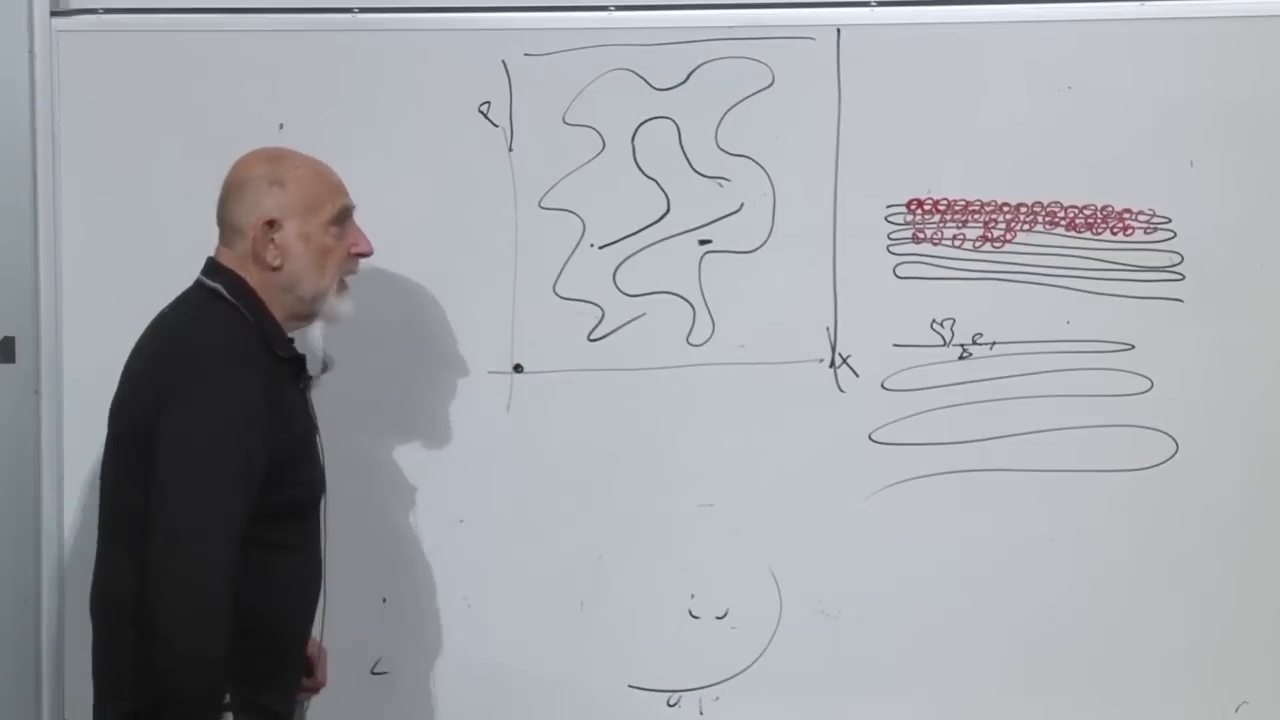
\includegraphics[width=0.90\textwidth]{lecture_07_figure_14.png}
\caption{一个紧致的特殊态在有界的可及区域中演化为复杂的细丝，而粗粒化元胞则散布到远为更大的面积上。}
\lectureframe{01:33:10}
\end{figure}

有两点限定条件很重要。混沌本身并不证明每条轨迹都会访问每个可及邻域；那个更强的采样主张需要遍历性或混合性。也并非每个物理系统都是混沌的。一般的多体气体和理想化台球提供了所设想的场景，在其中混合是一种有用的物理预期。

\section{回归并不消除不可逆性}

假设所有空气分子一开始都位于一个角落，并具有特别制备的速度模式。碰撞很快使它们散布到整个房间，粗粒化描述达到平衡。在有限保测度的相空间中，庞加莱回归定理表明，几乎每个初始点都会任意接近地回到其起点。对于容差\(\epsilon>0\)，在定理的假设下回归时间\(t_R(\epsilon)\)是有限的，尽管对于宏观系统它大得惊人。精确回到一个无限精确的点既非必需，通常也不被预期。

\begin{classroomqa}
\audiencequestion{在台球例子中，击打母球是否会注入能量并破坏封闭演化？}
\lecturerresponse{所选的初始态从击打之后立即开始，那份能量已经包含在内。回归涉及随后孤立的理想化台球动力学；回到初始态附近包括一种构型，其中母球在所选容差内接近球堆。
\lecturetimestamp{01:35:37--01:35:55}}
\end{classroomqa}

\begin{classroomqa}
\audiencequestion{如果气体最终能够回到角落，我们是否丢失了信息，系统是否真的可逆？}
\lecturerresponse{微观动力学始终是可逆的。粗粒化熵可以上升，因为我们不再分辨精细关联，然而一次极其罕见的涨落可以使系统回到其特殊初始宏观态附近。因此，回归与粗粒化不可逆性是相容的。
\lecturetimestamp{01:37:34--01:38:15}}
\end{classroomqa}

这引向玻尔兹曼的基本表述。熵并非在每一个逻辑上可能的瞬间都增加。给定一个大系统的非平衡宏观态，与之相容的微观延续中，压倒性地更多者通向更大的宏观态，而非通向更加特殊的宏观态。熵\emph{很可能}增加。向下的涨落和回归是允许的，但它们的概率和时间尺度使它们在通常的宏观经验中不可见。可逆性问题曾是统计力学历史上重大斗争之一，并沉重地压在玻尔兹曼身上。这一历史关联不应被变成关于他生平的简单因果主张。

\section{混沌意味着什么}

为了给出更具操作性的混沌定义，假设两个初始相点相差\(\delta\Gamma(0)\)，在线性化分离仍有意义的范围内，一个混沌方向通常满足
\begin{equation}
 \lVert\delta\Gamma(t)\rVert
 \sim e^{\lambda t}\lVert\delta\Gamma(0)\rVert,
 \qquad \lambda>0,
 \label{eq:sm7-lyapunov-growth}
\end{equation}
数\(\lambda\)是一个李雅普诺夫指数。要预测时间\(t\)，初始数据所需的精度大致按\(e^{-\lambda t}\)缩放。动力学定律的精度也很重要：模型误差会与初始条件误差一同被放大。天气就是人们熟悉的例子。

\begin{classroomqa}
\audiencequestion{是否存在一条原理，说明\emph{大多数}系统都是混沌的，还是说这仅仅是经验性的？}
\lecturerresponse{混沌与非混沌的哈密顿量都有无穷多个，甚至\emph{大多数}一词也需要在哈密顿量空间上给定一个测度。复杂的相互作用系统往往是混沌的，但并没有一个初等的普适判据，能仅凭检查就把每个哈密顿量分类。
\lecturetimestamp{01:39:27--01:40:49}}
\end{classroomqa}

\begin{classroomqa}
\audiencequestion{在这场讨论中，\emph{混沌}究竟是什么意思？}
\lecturerresponse{邻近的相轨迹分离得足够快，以至于长时间预测要求对初始条件的了解以指数方式改进。谐振子是相反的对照：相邻相点一起旋转并保持接近。精确的两体开普勒问题也是非混沌的，而一般三体问题则存在混沌区域。
\lecturetimestamp{01:40:50--01:43:45}}
\end{classroomqa}

\begin{classroomqa}
\audiencequestion{运动定律以及初始条件都必须知道到高精度吗？}
\lecturerresponse{是的。两种误差来源都会通过动力学传播，而混沌演化会把二者都放大。
\lecturetimestamp{01:43:46--01:43:55}}
\end{classroomqa}

双摆提供了一个生动的例子。普通摆是可积且可预测的。加上第二个摆后，起初几乎一起出发的轨迹最终可能以不同方式转移能量，并朝完全不同的方向运动。

\begin{figure}[t]
\centering
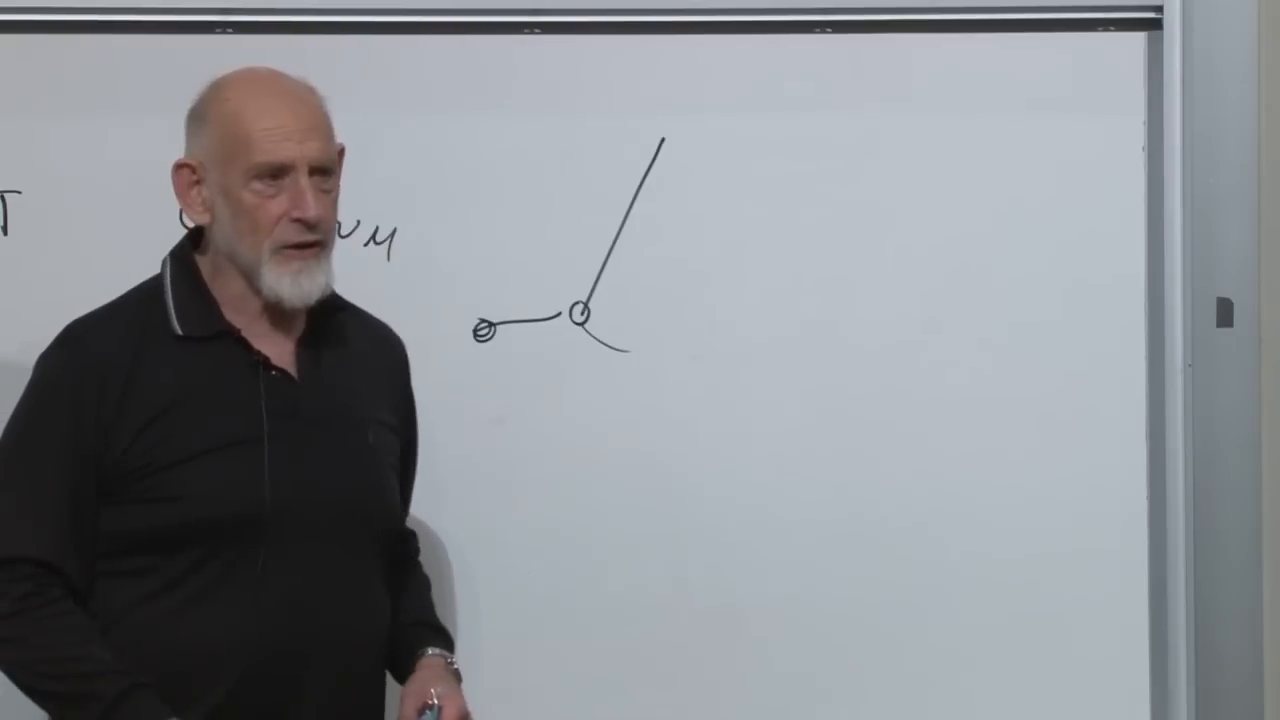
\includegraphics[width=0.90\textwidth]{lecture_07_figure_15.png}
\caption{双摆作为确定性混沌的一个具体例子。}
\lectureframe{01:44:40}
\end{figure}

\begin{classroomqa}
\audiencequestion{为什么一个力学系统可以是混沌的，而另一个却不是？}
\lecturerresponse{这是哈密顿量及其不变结构的性质，而不是摩擦或实验噪声的结果。判定这一点在数学上可能很困难；复杂性有提示作用，但并不是证明。
\lecturetimestamp{01:44:03--01:45:58}}
\end{classroomqa}

\begin{classroomqa}
\audiencequestion{没有摩擦的理想双摆仍然是混沌的吗？}
\lecturerresponse{是的。并不需要耗散。精确的确定性哈密顿运动可以对初始条件具有敏感依赖性。无限精度的初始数据会无限期地确定轨迹，但有限精度给出有限的预测时域。
\lecturetimestamp{01:45:57--01:47:54}}
\end{classroomqa}

\begin{classroomqa}
\audiencequestion{混沌与没有闭式解是同一回事吗？}
\lecturerresponse{不是。混沌系统通常缺乏全局有用的闭式轨迹，但解析可解性与敏感依赖性是两种不同的性质。混沌是通过轨迹分离在动力学上诊断出来的，而不仅仅是因为我们写不出公式。
\lecturetimestamp{01:48:20--01:49:23}}
\end{classroomqa}

\begin{classroomqa}
\audiencequestion{普遍存在的混沌与恰好平衡在不稳定的山顶上有什么不同？}
\lecturerresponse{山顶是一个例外的不稳定状态：离开它以后，邻近轨迹未必会迅速分离。在混沌区域中，不稳定性沿轨道是典型的，邻近相点会反复分离。正的李雅普诺夫指数刻画了这种持续增长。
\lecturetimestamp{01:49:27--01:50:11}}
\end{classroomqa}

\section{从微观运动到统计定律}

声速估计表明，微观热运动如何确定一个宏观传播尺度，而其中的问题则揭示出必须指定哪个热力学导数。随后，振子展示了经典能量均分所能达到的范围及其失效。量子能级间距冻结了刚性模式，解释了热容为何随温度变化，并阻止无穷多个高频模式携带无穷大的热能。

从精确的微观物理到有效宏观描述的同一递进过程，化解了第二定律核心处的表面矛盾。哈密顿流保持精确的相空间体积并且保持可逆。混沌拉伸产生的关联比宏观描述所保留的更精细，因此粗粒化后的占据区域会增长。回归性保证罕见的返回并非被禁止；概率解释了为什么它们不构成日常经验。第二定律并不是一种新的不可逆微观力。对于具有极多自由度的系统中特殊的宏观初始条件，它是演化过程压倒性地可靠的统计方向。
\chapter{递推、非平衡序与伊辛自旋}

\lectureoverview{从房间的一半释放出来的气体会迅速趋向平衡，然而可逆力学表明，足够长的演化也必定会产生向那个例外状态的回归。我们根据相空间体积估计回归时间，把递推与宇宙那个无法解释的低熵开端区分开来，并利用由此产生的谜题来讨论玻尔兹曼大脑、连贯的历史，以及由能量流维持的生命。随后我们转向磁序。独立的两态自旋给出一个可精确求解的热身例子：组合学决定了配分函数，而磁化强度是一个双曲正切。近邻相互作用最终恢复上--下对称性，并引出一维伊辛模型。}

\section{一屋子最终会回归的空气}

从房间左半边的所有空气开始。人们可以用一块隔板来制备这个状态：把右半边抽成真空，把空气放在左边，然后抽掉隔板。气体迅速扩散到整个房间并趋近热平衡。熵增加。没有发生任何令人惊讶的事情。

现在把房间密封起来并等待。连续一百万次正面朝上是一份极不可能的抛硬币记录，但一个无限重复的实验最终会产生极不可能的记录。同样的逻辑适用于气体。在某个遥远的时刻，它的所有分子将再次被发现位于左半边，或者位于某个同样特殊的区域。这样的回归就是庞加莱递推。

精确的定理比这幅图像要稍微谨慎一些。对于一个测度有限、其动力学保持相空间体积的相空间区域，几乎每一个初始点都会任意接近地回到它的出发点。像\emph{所有分子都在左半边}这样的宏观陈述则更容易：它只要求轨迹重新进入一个有限的粗粒化区域，而不要求每一个分子坐标都精确回归。实际的问题是这需要多长时间。

\subsection{一个高维相点}

对于\(N\)个经典粒子，相空间有\(6N\)个坐标，\begin{equation}
 \Gamma=(\bm x_1,\ldots,\bm x_N;\bm p_1,\ldots,\bm p_N).
 \label{eq:sm8-phase-point}
\end{equation}
位置受房间限制。在总能量固定时，动量也受到限制，因为一个粒子不可能携带任意大的动量而不携带任意大的能量。因此，在递推论证的假设下，允许的能量壳层具有有限的测度。

相点确定性地运动，但在多体气体中它的运动是混沌的。邻近的轨迹迅速分离，就像在一连串台球碰撞中那样。经过粗粒化之后，一条很长的轨迹看起来在可及区域内到处游荡。

\begin{figure}[t]
\centering
\includegraphics[width=0.90\textwidth]{lecture_08_figure_02.png}
\caption{一个示意性的相空间区域以及在其中游荡的复杂轨迹。这幅图被有意画成低维的；真实的气体生活在一个\(6N\)维空间中。}
\lectureframe{00:06:41}
\end{figure}

这幅低维草图立刻诱使我们犯一个错误。如果那个特殊状态占据了所画矩形的一半，人们可能会说气体应该有半数时间待在那里。但是\emph{每个分子都位于左半边}约束了每一个位置坐标，而不只是相点的一个坐标。

只取在一维空间中运动的两个粒子，坐标分别为\(x_1\)和\(x_2\)。它们的位形空间是一个正方形。要求\(x_1<L/2\)选出正方形的一半；同时要求\(x_1<L/2\)和\(x_2<L/2\)则选出一个四分之一：
\begin{equation}
 P_2=\frac{1}{2}\frac{1}{2}=\frac{1}{4}.
 \label{eq:sm8-two-particle-quarter}
\end{equation}

\begin{figure}[t]
\centering
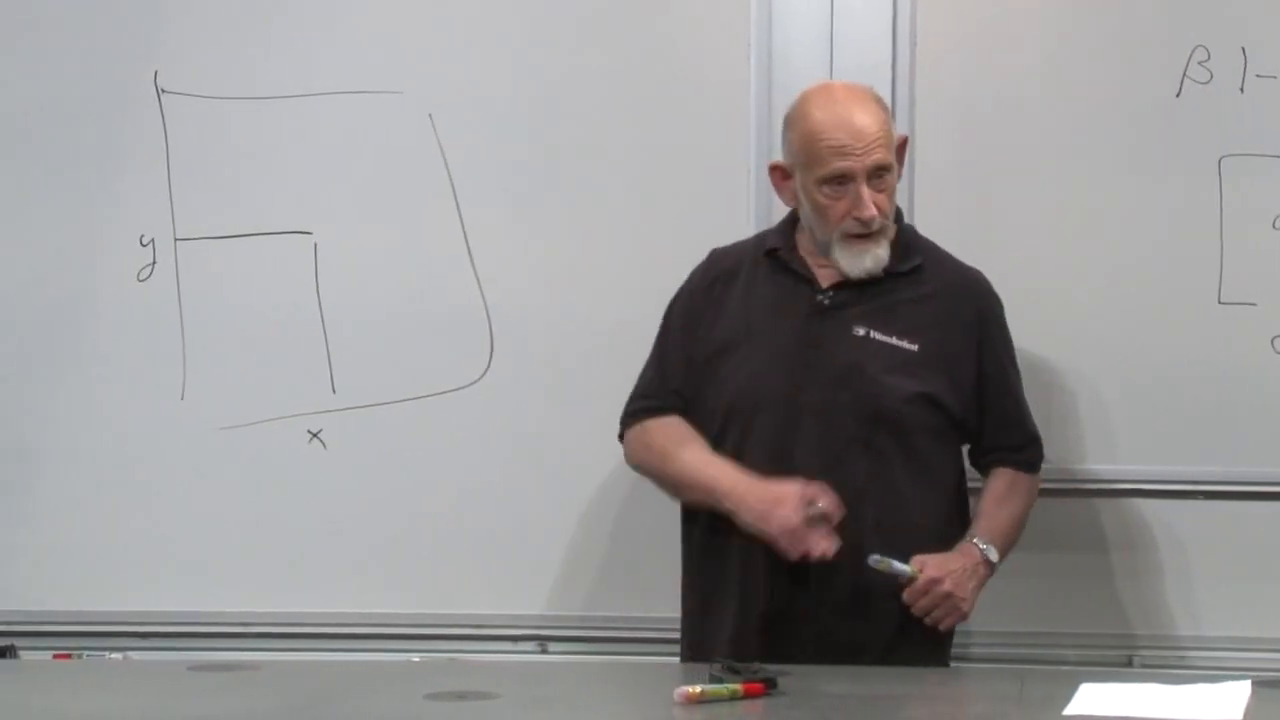
\includegraphics[width=0.90\textwidth]{lecture_08_figure_07.png}
\caption{对于两个一维粒子，较小的正方形代表两个坐标都位于房间所选那一半中的位形。}
\lectureframe{00:07:08}
\end{figure}

三个粒子给出\(1/2^3\)，而\(N\)个粒子给出
\begin{equation}
 P_{\mathrm{half}}(N)
 =\left(\frac{1}{2}\right)^N.
 \label{eq:sm8-half-probability}
\end{equation}
指数就是全部要点。一个二分之一因子很平常；二分之一的一个宏观粒子数次幂则超出了平常的直觉。

\begin{classroomqa}
\audiencequestion{答案难道不应该是\(1/3^N\)吗，因为分子还有其他空间方向？}
\lecturerresponse{这取决于所施加的条件。如果唯一的问题是每个粒子是否都位于分隔墙的左侧，那么每个粒子满足一个二元条件，答案就是\(2^{-N}\)。如果再约束其可用位置空间中另一个独立的分数，就会再提供一个因子。
\lecturetimestamp{00:07:47--00:08:05}}
\end{classroomqa}

\section{相体积、熵与递推尺度}

同一个估计也可以不借助“一半”来写出。设房间具有普通空间体积\(V\)，并设\(v\)为一个较小的区域，我们要求在其中找到每一个分子。忽略两个宏观态共有的动量因子后，可用的位形空间体积为
\begin{equation}
 \Omega_{\mathrm{room}}\propto V^N,
 \qquad
 \Omega_{\mathrm{small}}\propto v^N.
 \label{eq:sm8-config-volumes}
\end{equation}
因此，长时间中处于小宏观态的比例为
\begin{equation}
 P(v)
 =\frac{\Omega_{\mathrm{small}}}{\Omega_{\mathrm{room}}}
 =\left(\frac{v}{V}\right)^N.
 \label{eq:sm8-volume-ratio}
\end{equation}

\begin{figure}[t]
\centering
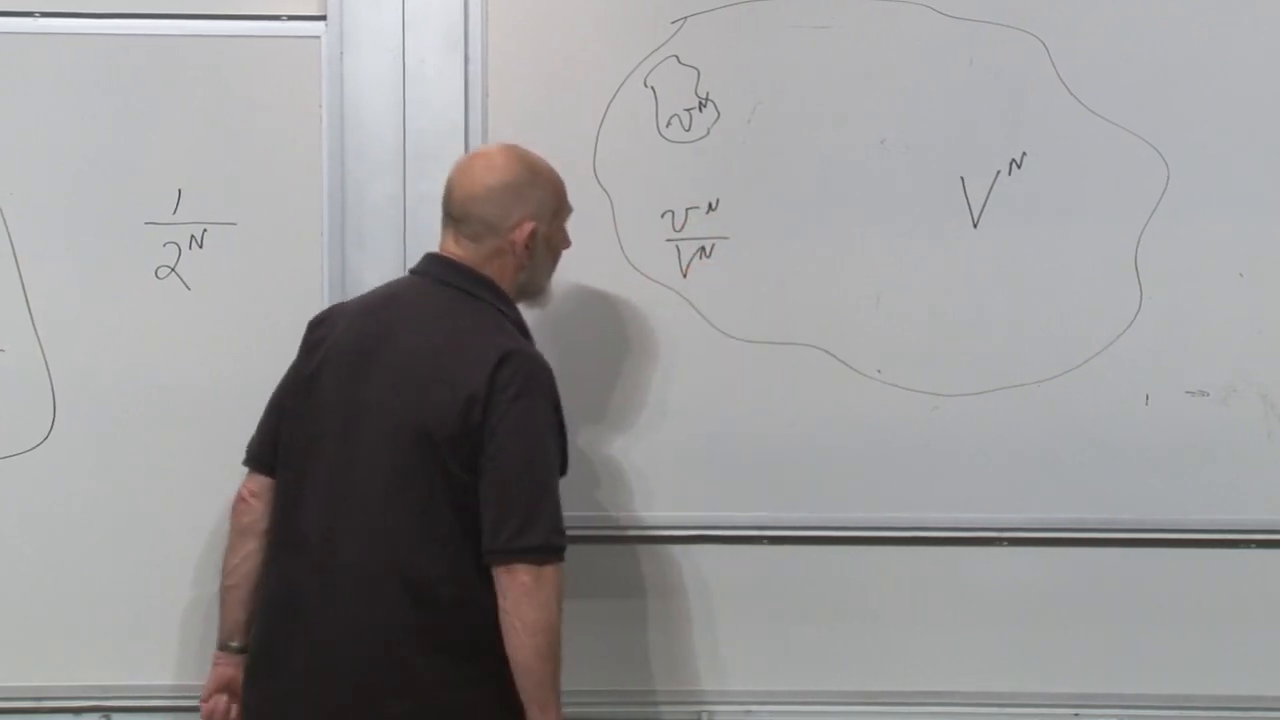
\includegraphics[width=0.90\textwidth]{lecture_08_figure_08.png}
\caption{黑板上的普遍相体积图像：可及区域\(V^N\)内部的一个小区域\(v^N\)，其比值为\(v^N/V^N\)。}
\lectureframe{00:10:44}
\end{figure}

在\(k_B=1\)的单位制下，熵是可及相体积的对数。若\(S_A=\log\Omega_A\)是受约束宏观态的熵，而\(S_{\rm eq}=\log\Omega_{\rm eq}\)是平衡态的熵，则
\begin{equation}
 \begin{aligned}
 P(A)
 &=\frac{\Omega_A}{\Omega_{\rm eq}}\\
 &=\exp\!\left(S_A-S_{\rm eq}\right)\\
 &=e^{-\Delta S},\\
 \Delta S&=S_{\rm eq}-S_A.
 \end{aligned}
 \label{eq:sm8-entropy-probability}
\end{equation}
对于半房间态，\(\Delta S=N\log 2\)，而\eqref{eq:sm8-entropy-probability}恰好化为\(2^{-N}\)。简写\(P\sim e^{-S_{\rm eq}}\)仅在把特殊区域的熵当作固定参考时才适用；具有物理意义的指数是熵亏损\(\Delta S\)。

\begin{classroomqa}
\audiencequestion{这是位形空间的体积，而不是整个相空间的体积吗？}
\lecturerresponse{对于这一比较而言，是的。我们施加的是位置条件，同时让动量分布保持在同一温度，因此共同的动量空间因子相消。完全一般的复现陈述使用相空间；而这个特定的概率可以由位形空间比值算出。
\lecturetimestamp{00:11:21--00:11:40}}
\end{classroomqa}

假设系统在微观关联时间或混合时间\(\tau_{\rm mix}\)上失去对其详细位置的记忆。那么，概率为\(P(A)\)的稀有区域会在如下尺度上被遇到：
\begin{equation}
 \tau_{\rm rec}
 \sim \frac{\tau_{\rm mix}}{P(A)}
 \sim \tau_{\rm mix}e^{\Delta S}.
 \label{eq:sm8-recurrence-time-general}
\end{equation}
对于半房间条件，
\begin{equation}
 \tau_{\rm rec}\sim\tau_{\rm mix}2^N.
 \label{eq:sm8-recurrence-time-half}
\end{equation}
讲座使用了刻意粗略的房间尺度估计\(N\sim10^{30}\)，给出令人难忘的尺度
\(\tau_{\rm rec}/\tau_{\rm mix}\sim2^{10^{30}}\)。在普通大气密度下，一个房间更接近\(10^{27}\)个分子，但把\(10^{30}\)换成\(10^{27}\)不会改变任何结论：复现时间仍然比宇宙年龄大得无法想象。

\begin{classroomqa}
\audiencequestion{复现时间以什么单位测量？从秒改成小时，或改成一个极短的单位，会改变结论吗？}
\lecturerresponse{量纲前因子是\(\tau_{\rm mix}\)；巨大的数是无量纲比值\(\tau_{\rm rec}/\tau_{\rm mix}\)。把秒改成小时只是除以一个普通的换算因子，与\(2^{10^{30}}\)相比可以忽略。单次访问角落的持续时间确实取决于分子速率。这个估计关心的是这种访问多么罕见地开始。还存在量子复现定理，但这里不需要它。
\lecturetimestamp{00:17:24--00:19:18}}
\end{classroomqa}

\begin{classroomqa}
\audiencequestion{计算一个任何实验都不可能等待的时间，目的何在？}
\lecturerresponse{要点是概念性的。它告诉我们，封闭的力学系统在何种意义上保持可逆。它几乎全部时间都待在平衡态附近，但在足够长的尺度上，它也会向低熵方向发生涨落。因此，第二定律是一个关于特殊初始数据的、概率上压倒性的陈述，而不是一条禁止反向运动的微观方程。
\lecturetimestamp{00:15:12--00:16:35}}
\end{classroomqa}

\section{可逆性与特殊的开端}

有意地从微小的半房间区域出发。几乎每一条邻近轨道都会立刻离开它，因为外面的相体积远多于里面。气体迅速扩散，然后等待极长的时间才返回。快速弛豫与漫长等待之间的这种不对称并不违反可逆力学。

快速逃逸的时间反演并不是整个等待期。它是短暂且协调得不可思议的一段过程：看起来处于平衡的分子速度恰好自行安排，使气体\emph{嗖地}冲进房间的一半。在普通逃逸结束时把每个动量都反向，气体就会反向重演逃逸过程。漫长的等待时间，就是那种特殊的入射速度模式自发出现所需的时间。

\begin{classroomqa}
\audiencequestion{时间对称性是否意味着缓慢复现到角落所需的时间，与最初从那里逃逸所需的时间一样长？}
\lecturerresponse{不是。把逃逸与其精确的时间反演相比较。两者都很快。花费巨大时间的是在平衡态中等待那个引发反向嗖地冲入的精确入射涨落。在极其漫长的记录中，偏离平衡的远足会沿两个时间方向发生，其局部历史是对称的。
\lecturetimestamp{00:20:46--00:21:58}}
\end{classroomqa}

因此，复现论证只能解释时间箭头的一部分。它解释了为什么在系统始于低熵区域的\emph{给定条件}下，熵通常会上升。它并不解释为什么初始条件是特殊的。在宇宙学中，这个缺失的前提变成了核心问题：为什么可观测宇宙会始于其引力相空间中如此异常小的一个区域？

\begin{classroomqa}
\audiencequestion{复现是否适用于宇宙学？在宇宙扩散开来之后，如果等待足够久，它是否可能复现？}
\lecturerresponse{这个问题无法回避，但其答案取决于整体宇宙学。一个真正封闭、具有有限平衡态空间的系统会倾向于复现。膨胀的时空、引力、视界，以及无限或非定常的状态空间，都可能改变前提。这里重要的教训更为狭窄：仅凭平衡态复现图景，并不足以对我们所看到的这个有结构的宇宙给出令人满意的统计解释。
\lecturetimestamp{00:19:59--00:20:45}}
\end{classroomqa}

\begin{classroomqa}
\audiencequestion{复现是否依赖于一开始把气体制备在一个小区域中？如果房间从平衡态开始，空气最终仍然会聚集到一个角落吗？}
\lecturerresponse{会。复现涉及封闭系统的长时间动力学，因此一个看起来处于平衡态的初始态也会经历罕见的低熵涨落。制备半房间状态之所以重要，是出于另一个原因：它让我们能够以已知的特殊初始状态为条件，并追问为什么熵在此后立即上升。
\lecturetimestamp{00:22:04--00:22:20}}
\end{classroomqa}

\section{为什么随机涨落所预言的东西太少}

人们可能会试图把复现变成一种宇宙学：也许宇宙几乎全部永恒时间都处于平衡态，而我们当前的世界是一次罕见的涨落。这个提议未能通过一项尖锐的统计检验。以观察者的存在为条件，然后追问该观察者还应当预期看到什么。

大到足以形成一个行星的涨落极其罕见。形成两个行星的涨落需要更大的熵亏缺，因而更加罕见。形成恒星、星系、宇宙微波背景，以及关于漫长过去且彼此一致的记录的涨落，则还要罕见得多，多出一个巨大的额外指数因子。因此，平衡态涨落理论预言的是足以供观察的最小涨落，而不是实际观察到的这个丰富而连贯的世界。在其最极端的形式中，最小的观察者被称为玻尔兹曼大脑。

其逻辑是条件概率。令\(A\)表示发生一次观察者尺度涨落的事件，\(B\)表示一个独立的第二结构。如果二者都具有微小概率\(p\)，那么
\begin{equation}
 P(B\mid A)=p,
 \qquad
 P(A\cap B)=p^2.
 \label{eq:sm8-conditional-fluctuations}
\end{equation}
得知第一次涨落已经发生，并不会使第二次涨落变得可能。彩票类比在这个层面上是精确的：先前的中奖者在下一次独立抽奖中并没有更高的机会。因此，观察者可以以自身存在为条件，但仍然应当惊讶地发现自己身处一个独立地具有结构的环境之中。

\begin{classroomqa}
\audiencequestion{既然一个行星或一个玻尔兹曼观察者已经存在，另一个的概率真的更小吗？}
\lecturerresponse{第二个独立罕见涨落的条件概率仍是同一个微小的一次事件概率，而不是它的平方。二者同时发生的联合概率才是平方。这正是为什么第一个观察者仍应预期自身之外是热无序的。发现一个配偶、另一个行星，以及一片有序的天空，都是反对如下前提的证据：该观察者是由一次孤立的平衡态涨落组装而成的。
\lecturetimestamp{00:26:12--00:30:27}}
\end{classroomqa}

\subsection{关于过去的连贯记录}

同样的论证也适用于历史。两本彼此一致的教科书、符合同一膨胀历史的天文记录、地质地层、记忆和实验室笔记本，都会彼此约束。一本随机出现的教科书可以包含任何故事。而一整套关于同一过去且彼此一致的记录网络，则占据一个小得多的相空间区域。

课堂例子使用了那个熟悉的传说：乔治·华盛顿砍倒了一棵樱桃树。这个传说是否真实无关紧要。要点在于，在一个于当前瞬间涨落而存在的世界中，一本书中的句子并没有给出任何动力学理由，使另一条记录与它一致。连贯的关联是共同历史的证据，而不仅仅是一次瞬时意外的证据。

\begin{classroomqa}
\audiencequestion{这里的\emph{历史一致性}是什么意思？}
\lecturerresponse{它意味着，当前的许多记录作为共同过去的后果而彼此吻合。涨落可以伪造记录和记忆，但伪造一个相互一致的网络所需的涨落，要比伪造一个最小观察者大得多。因此，复现理论预言，大多数类似观察者的涨落并不具备我们实际发现的那种一致性。
\lecturetimestamp{00:30:30--00:31:12}}
\end{classroomqa}

\begin{classroomqa}
\audiencequestion{宇宙是否仍可能是一个封闭系统，只不过其平衡化时间和复现时间极其漫长？}
\lecturerresponse{这种可能性并不能消除统计问题。在无限漫长的历史中，会出现许多类似观察者的涨落，而其中绝大多数都是没有一致周围历史的最小涨落。从那个系综中选出的一个观察者，不应期望看到我们的观测结果。因此，宇宙学家把玻尔兹曼大脑问题当作对宇宙学测度和晚期模型的检验来认真对待，而不是把它当作复现已经被观测到的断言。
\lecturetimestamp{00:31:13--00:32:42}}
\end{classroomqa}

\section{作为由流动维持的结构之生命}

生命似乎提出了相反的困难。有机体在长时间内维持着精巧的组织；它们看起来不像短暂的偶然涨落。解决之道在于，第二定律适用于完整的封闭系统。一个子系统可以降低或维持其熵，只要其环境中发生更大的熵增：
\begin{equation}
 \dot S_{\rm total}
 =\dot S_{\rm subsystem}+\dot S_{\rm environment}\geq 0.
 \label{eq:sm8-open-system-second-law}
\end{equation}

地球并不处于热平衡。在人类的时间尺度上，它近似是定常的，但定常并不意味着静止。能量流经它。阳光到达，经过许多过程被降级，并以较低的有效温度辐射出去。这种流通可以在总熵上升的同时维持局部的组织。

水流过管道提供了最直接的力学图像。流动中可以包含持续存在的涡旋和旋涡。它们是有组织的结构，但它们由水流维持。把两端封住，停止流动，随着水趋近于沉闷的平衡，黏性会抹去这些涡旋。流出的水比流入的水更暖，因此更大的系统已经支付了熵的账单。

\begin{classroomqa}
\audiencequestion{生命会降低熵吗？为什么它的组织能够持续存在，而不是像普通涨落那样出现又消失？}
\lecturerresponse{生命可以在局部维持或降低熵，但只能通过输出更多的熵来实现。它的持续存在来自一种定常的非平衡流动，主要是太阳能流经地球的流动。如果地球对入射和出射辐射都是封闭的，它最终会趋近热平衡，而有组织的活动将会停止。生命更接近于溪流中的一个涡旋，而不是一个平衡涨落。
\lecturetimestamp{00:32:43--00:35:42}}
\end{classroomqa}

至此，我们离开\emph{有趣的东西}，并回到讲座中刻意平淡的说法：某种乏味的东西——磁体。

\section{冷却磁体：磁畴与一个被选定的方向}

统计力学常常把一个数学模型称为磁体，即使它并不是一块字面意义上的铁。有用的共同特征是，一组能够发生有序化的局域自由度。在真实的磁性材料中，这些自由度可能来自原子磁矩、电子自旋、轨道电流或晶体单元的有效磁矩。

在高温下，热无序使局域磁矩指向许多方向，从而给出很小或没有净磁化。如果相邻磁矩在排列一致时能量更低，那么冷却就允许小的排列一致的磁畴形成。进一步冷却使能量优势更加重要，关联磁畴随之长大。在支持铁磁相变的系统中，关联长度在有限的临界温度处变为宏观尺度。于是，有序相会选择一个取向，尽管零场能量事先并不偏好某一个取向。

\begin{classroomqa}
\audiencequestion{微观磁体是否应当因为北极吸引南极而倾向于反向排列？}
\lecturerresponse{有效相互作用取决于材料。普通的偶极子直觉并不是整个微观问题；交换作用、晶体结构和相互竞争的相互作用都很重要。铁磁材料是那些有效低能倾向有利于平行排列的材料，而其他材料则可能有利于反向排列。
\lecturetimestamp{00:39:56--00:40:30}}
\end{classroomqa}

\begin{classroomqa}
\audiencequestion{为了使磁矩排列整齐，材料冷却时是否必须存在外磁场？}
\lecturerresponse{不需要。相互作用无需磁场即可产生有序。在完全对称的理想化情形中，不同方向在能量上等价，因此实际实现的方向由初始涨落、边界或任意小的杂散场选定。从这些等价方向中选定一个，就是自发对称破缺；宏观有序的出现就是磁性相变。
\lecturetimestamp{00:40:31--00:42:33}}
\end{classroomqa}

真实材料很复杂，因此我们现在做极端的简化。每个局域磁矩只能向上或向下：
\begin{equation}
 \sigma_i=+1\quad\hbox{or}\quad\sigma_i=-1.
 \label{eq:sm8-ising-spin}
\end{equation}
这个模型中没有东或西。两个允许的取向是模型的定义，正如正面和反面是抛硬币的两个结果。其价值不在于微观真实性，而在于数学上的清晰性，以及它能够表示许多系统共有的有序化现象。

\begin{classroomqa}
\audiencequestion{这两个态的对象在物理上是什么？应该把它们想象成粒子吗？}
\lecturerresponse{可以想象晶体格点上的原子，每个原子具有由自旋或微观电流产生的有效磁矩。然而，对于这个模型而言，只有这个二值变量才是重要的。限制为向上和向下，是为了使统计力学变得简单。
\lecturetimestamp{00:44:22--00:45:01}}
\end{classroomqa}

\section{外场中的独立自旋}

第一个模型包含\(N\)个彼此不相互作用的自旋。外场\(H\)提供了唯一的能量尺度，而\(\mu\)衡量一个自旋与其耦合的强度。我们保留计算中使用的符号约定：
\begin{equation}
 \epsilon_i=\mu H\sigma_i.
 \label{eq:sm8-single-spin-energy}
\end{equation}
对于\(H>0\)，向上自旋\(\sigma_i=+1\)的能量为\(+\mu H\)，而向下自旋\(\sigma_i=-1\)的能量为\(-\mu H\)。因此，这一约定使正场有利于向下自旋。它与另一种常见的命名约定相反，但只要符号使用一致，物理就不依赖于名称。

设\(n\)为向上自旋的数目，\(m\)为向下自旋的数目。则
\begin{equation}
 n+m=N,
 \qquad
 E=(n-m)\mu H.
 \label{eq:sm8-counting-energy}
\end{equation}

\begin{figure}[t]
\centering
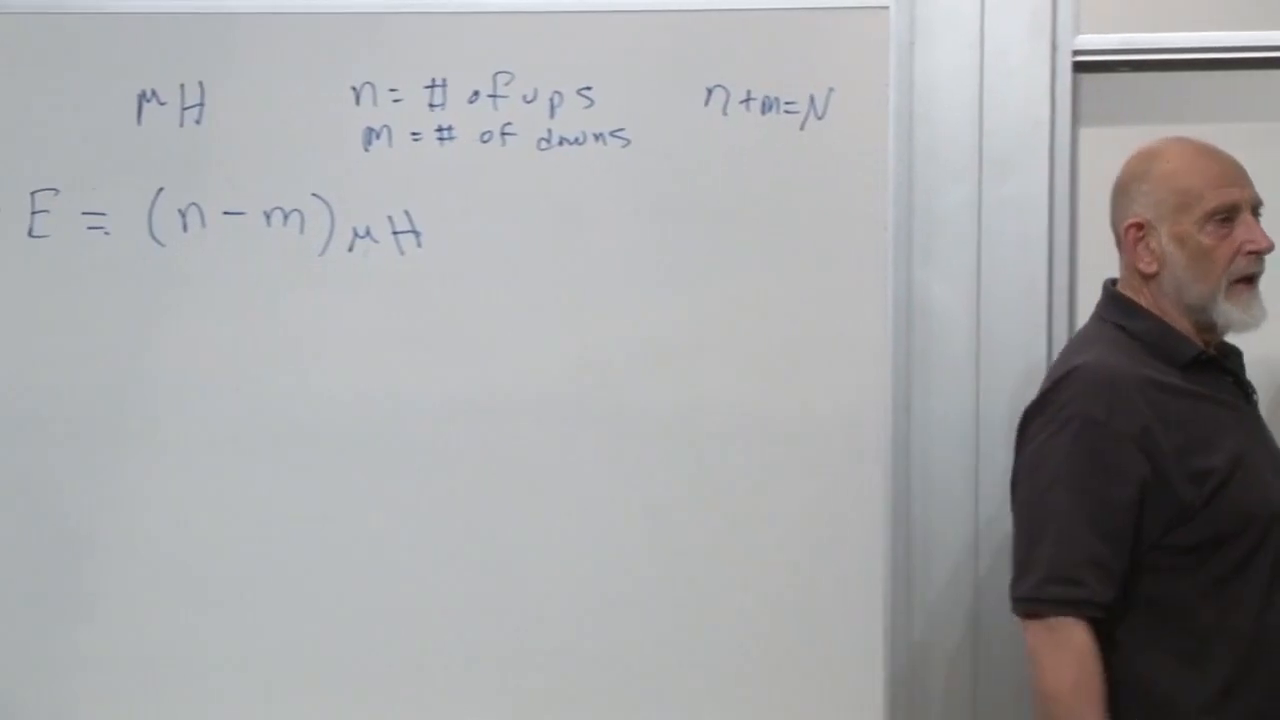
\includegraphics[width=0.90\textwidth]{lecture_08_figure_03.png}
\caption{独立自旋设置：\(n\)个向上自旋，\(m\)个向下自旋，\(n+m=N\)，以及\(E=(n-m)\mu H\)。}
\lectureframe{00:49:50}
\end{figure}

\begin{classroomqa}
\audiencequestion{\(H\)、\(\mu\)和\(E\)的量纲是什么？\(H\)是一个数还是磁场？}
\lecturerresponse{\(H\)表示外部施加的场强，\(\mu\)表示磁矩。它们的乘积\(\mu H\)具有能量的量纲。在抽象模型中，人们常将它们合并为一个能量值的参数，习惯上也用小写\(h\)表示。这里我们保留两个因子以显示其物理来源，而\(E\)是总能量。
\lecturetimestamp{00:48:21--00:49:27}}
\end{classroomqa}

\subsection{组态计数}

对于固定的\(n\)和\(m=N-n\)，选择\(N\)个格点中的哪\(n\)个向上。多重性为
\begin{equation}
 \Omega(n,m)=\binom{N}{n}
 =\frac{N!}{n!\,m!}.
 \label{eq:sm8-spin-multiplicity}
\end{equation}
这些组态中的每一个都具有相同的能量
\eqref{eq:sm8-counting-energy}。

\begin{classroomqa}
\audiencequestion{既然\(n\)和\(m\)并不独立，它们能同时作为求和指标吗？组合因子又出现在哪里？}
\lecturerresponse{它们可以写成一个受约束的对，满足\(n+m=N\)，或者可以对\(n=0,\ldots,N\)求和并令\(m=N-n\)。玻尔兹曼权重属于每一个单独的组态；将同一能量的所有组态归并在一起，会使该权重乘以\(N!/(n!\,m!)\)。
\lecturetimestamp{00:52:04--00:53:03}}
\end{classroomqa}

因此配分函数为
\begin{align}
 Z_N
 &=\sum_{n+m=N}
   \frac{N!}{n!\,m!}
   e^{-\beta\mu H(n-m)}
 \notag\\
 &=\sum_{n=0}^{N}
   \binom{N}{n}
   \left(e^{-\beta\mu H}\right)^n
   \left(e^{+\beta\mu H}\right)^{N-n}.
 \label{eq:sm8-spin-z-sum}
\end{align}
引入
\begin{equation}
 x=e^{-\beta\mu H},
 \qquad
 y=e^{+\beta\mu H}.
 \label{eq:sm8-xy}
\end{equation}
二项式定理随即完成计算：
\begin{align}
 Z_N
 &=\sum_{n=0}^{N}\binom{N}{n}x^n y^{N-n}
   =(x+y)^N
 \notag\\
 &=\left(e^{-\beta\mu H}+e^{+\beta\mu H}\right)^N
   =\left[2\cosh(\beta\mu H)\right]^N.
 \label{eq:sm8-spin-z-closed}
\end{align}

\begin{figure}[t]
\centering
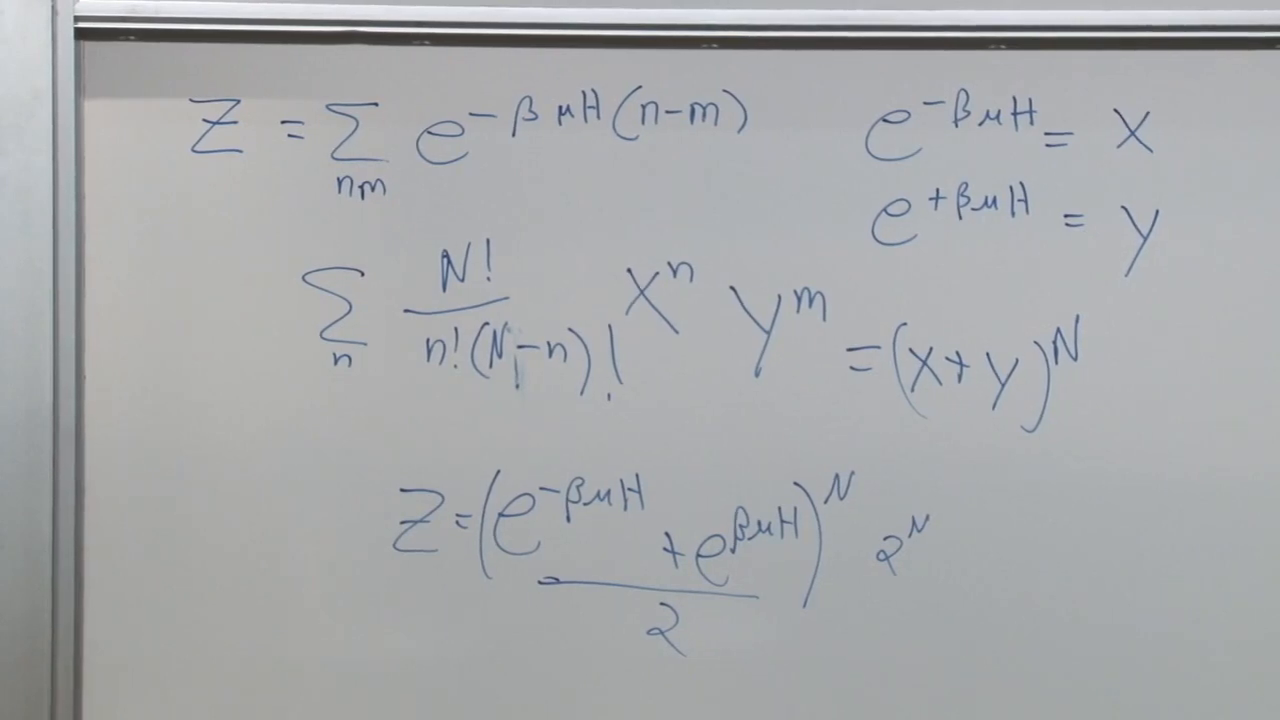
\includegraphics[width=0.90\textwidth]{lecture_08_figure_04.png}
\caption{配分函数求和、代换\(x\)和\(y\)，以及二项式约化为\(2\cosh(\beta\mu H)\)的幂。}
\lectureframe{00:56:00}
\end{figure}

还有一个更简短的推导。由于自旋是独立的，一个自旋有
\begin{equation}
 z_1=e^{-\beta\mu H}+e^{+\beta\mu H}
    =2\cosh(\beta\mu H),
 \label{eq:sm8-one-spin-z}
\end{equation}
以及\(Z_N=z_1^N\)。尽管如此，组合推导仍值得保留，因为它明确显示了多重性如何与能量竞争。

\section{组态磁化强度与系综磁化强度}

对于一个组态，定义其每格点的无量纲自旋过剩为
\begin{equation}
 M_{\rm conf}=\frac{n-m}{N}.
 \label{eq:sm8-config-magnetization}
\end{equation}
它的范围从全部自旋向上时的\(+1\)到全部自旋向下时的\(-1\)。这里使用的热力学磁化强度是其玻尔兹曼平均值，
\begin{equation}
 M=\left\langle M_{\rm conf}\right\rangle
  =\left\langle\frac{n-m}{N}\right\rangle.
 \label{eq:sm8-average-magnetization}
\end{equation}
因子\(\mu H\)不属于这个定义。它在计算过程中曾被短暂地写在那里，随后被去掉；\(\mu H\)将自旋过剩转换为能量。

逐组态地，
\begin{equation}
 E=N\mu H M_{\rm conf}.
 \label{eq:sm8-energy-config-m}
\end{equation}
求平均的线性性立即给出
\begin{equation}
 \langle E\rangle=N\mu H M.
 \label{eq:sm8-energy-average-m}
\end{equation}

\begin{figure}[t]
\centering
\includegraphics[width=0.90\textwidth]{lecture_08_figure_05.png}
\caption{自旋行、修正后的平均磁化强度，以及黑板上强调的能量关系。}
\lectureframe{01:01:22}
\end{figure}

\begin{classroomqa}
\audiencequestion{磁化强度是被赋予某个特定构型，还是我们在讨论平均磁化强度？为什么同样的关系对平均能量也成立？}
\lecturerresponse{两种概念都出现了，应当加以区分。\((n-m)/N\) 是一个构型中的取值；\(M\) 是它的玻尔兹曼平均。由于 \(E=N\mu H M_{\rm conf}\) 在每个构型中分别成立，用相同的概率对两边取平均便得到 \(\langle E\rangle=N\mu H M\)。固定量 \(N\)、\(\mu\) 和 \(H\) 穿过平均运算。
\lecturetimestamp{00:59:54--01:03:40}}
\end{classroomqa}

\begin{classroomqa}
\audiencequestion{这个模型如何能让每个自旋都沿北--南方向排列，而不偏向向上或向下？}
\lecturerresponse{没有东和西是两态模型本身所固有的；这是对允许自由度的限制。当前的外场模型 \emph{确实}在向上与向下之间有所偏向：按照我们的符号约定，外场降低向下自旋的能量。因此这个模型没有上--下对称性。下面引入的零场伊辛模型将恢复这种对称性。
\lecturetimestamp{01:03:41--01:04:53}}
\end{classroomqa}

\subsection{由配分函数求能量}

平均能量由通常的恒等式给出
\begin{equation}
 \langle E\rangle
 =-\frac{\partial}{\partial\beta}\log Z_N.
 \label{eq:sm8-energy-identity}
\end{equation}
利用 \eqref{eq:sm8-spin-z-closed}，
\begin{align}
 \log Z_N
 &=N\log 2+N\log\!\left[\cosh(\beta\mu H)\right],
 \notag\\
 \langle E\rangle
 &=-N\mu H\,
   \frac{\sinh(\beta\mu H)}{\cosh(\beta\mu H)}
 \notag\\
 &=-N\mu H\tanh(\beta\mu H).
 \label{eq:sm8-average-energy}
\end{align}
将其与 \eqref{eq:sm8-energy-average-m} 结合便得到
\begin{equation}
 \boxed{M=-\tanh(\beta\mu H)}.
 \label{eq:sm8-magnetization-tanh}
\end{equation}

答案的形状中蕴含着物理。回忆
\begin{equation}
 \cosh x=\frac{e^x+e^{-x}}{2},
 \qquad
 \sinh x=\frac{e^x-e^{-x}}{2}.
 \label{eq:sm8-hyperbolic-definitions}
\end{equation}
在原点附近，\(\tanh x=x+O(x^3)\)；对于大的正 \(x\)，它趋近于 \(1\)。由于 \(\beta=1/T\)，
\begin{equation}
 M\longrightarrow -1
 \quad (T\longrightarrow0),
 \qquad
 M\longrightarrow 0
 \quad (T\longrightarrow\infty).
 \label{eq:sm8-magnetization-limits}
\end{equation}
在零温下，每个自旋都占据能量较低的向下态。在无穷大温度下，所有构型都变得等权重，外场偏向被抹平。反转 \(H\) 会反转 \(M\)。

\begin{figure}[t]
\centering
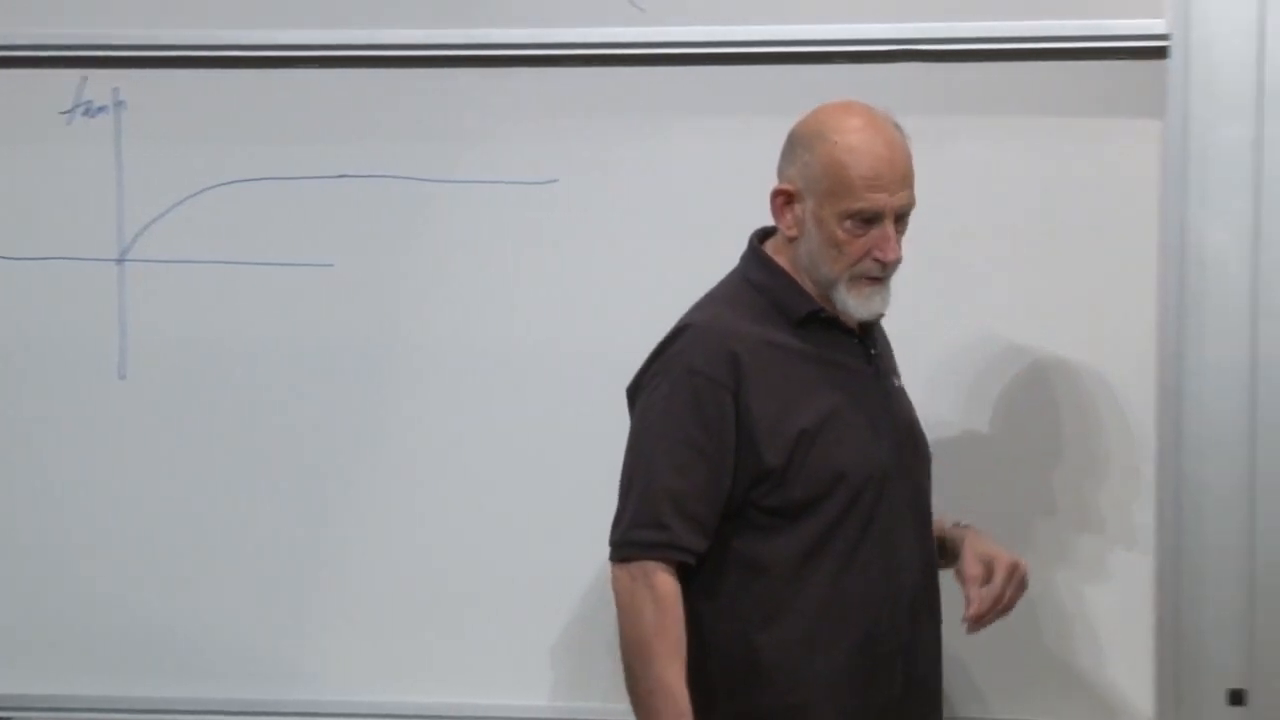
\includegraphics[width=0.90\textwidth]{lecture_08_figure_09.png}
\caption{双曲正切曲线在大的 \(\beta\mu H\) 下趋近于常数，并在原点附近呈线性。按照讲座的约定，物理磁化强度是所绘 \(\tanh\) 的负值。}
\lectureframe{01:13:14}
\end{figure}

\begin{classroomqa}
\audiencequestion{磁化强度连续变化。前面提到的相变温度在哪里？}
\lecturerresponse{在这个模型中没有相变温度。处于非零外场中的独立自旋太简单了，而且 \(\log Z_N=N\log[2\cosh(\beta\mu H)]\) 在每个有限正温度下都是光滑的。相变需要我们现在要接近的、有相互作用且对称的问题；二维零场伊辛模型是这一族中第一个具有有限温度相变的成员。
\lecturetimestamp{01:14:47--01:15:11}}
\end{classroomqa}

\section{伊辛模型：相邻对中的能量}

外场在统计开始之前就选定了一个方向。去掉这个场，让相邻自旋彼此提供有效场。如果某个格点的两个邻居都指向上，它们就偏向向上；如果两个都指向下，它们就偏向向下；如果一个指向上、一个指向下，那么在最简单的图像中它们的效果相互抵消。现在能量与对相关联，而不是与孤立格点相关联。

对于两个相邻自旋，取 \(J>0\) 并写出
\begin{equation}
 E_{12}=-J\sigma_1\sigma_2.
 \label{eq:sm8-pair-energy}
\end{equation}
取向一致的自旋有 \(\sigma_1\sigma_2=+1\) 和能量 \(-J\)；取向相反的自旋有乘积 \(-1\) 和能量 \(+J\)。因此，负号正是使该相互作用成为铁磁性的原因。

\begin{figure}[t]
\centering
\includegraphics[width=0.90\textwidth]{lecture_08_figure_06.png}
\caption{局域铁磁相互作用
\(E_{12}=-J\sigma_1\sigma_2\)。}
\lectureframe{01:19:59}
\end{figure}

在开放的一维链上，哈密顿量为
\begin{equation}
 {\cal H}=-J\sum_{i=1}^{N-1}\sigma_i\sigma_{i+1}.
 \label{eq:sm8-ising-chain-open}
\end{equation}
在周期性边界条件下，取 \(\sigma_{N+1}=\sigma_1\) 并对 \(N\) 求和。两种约定都把每个相邻对计数一次；对于长链，它们的边界差异变得可以忽略。

\begin{figure}[t]
\centering
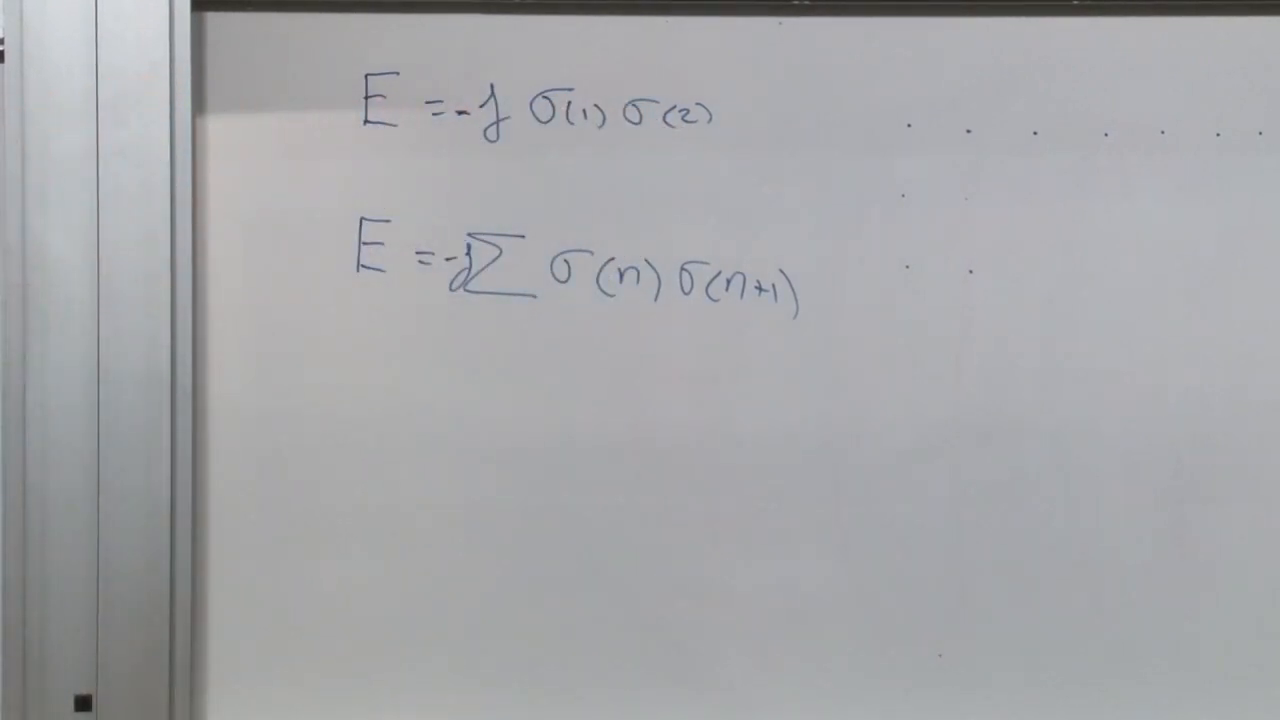
\includegraphics[width=0.90\textwidth]{lecture_08_figure_10.png}
\caption{局域对能量被推广到最近邻链哈密顿量。}
\lectureframe{01:20:46}
\end{figure}

在无穷大温度下，每个自旋串都等概率。平均而言，一半键取向一致，一半键取向相反，因此
\begin{equation}
 \left\langle\sigma_i\sigma_{i+1}\right\rangle_{T=\infty}=0,
 \qquad
 \left\langle{\cal H}\right\rangle_{T=\infty}=0.
 \label{eq:sm8-infinite-t-bond}
\end{equation}
这里的零能量并不是低能态。全部取向一致的基态每键能量为 \(-J\)，所以无穷大温度系综位于比它高出一个广延能量的位置。

\begin{classroomqa}
\audiencequestion{当每个单独的乘积 \(\sigma_i\sigma_{i+1}\) 要么是 \(+1\) 要么是 \(-1\) 时，平均乘积怎么会是零？}
\lecturerresponse{平均值不必是单个构型中所取的某个值。在无穷大温度下，取向一致和取向相反的键出现得同样频繁，因此它们的 \(+1\) 和 \(-1\) 贡献相互抵消。对磁化强度重要的那种平均区分在这里同样重要。
\lecturetimestamp{01:21:39--01:22:37}}
\end{classroomqa}

\subsection{两个基态与一个全局对称性}

在零温下，每个键都希望对齐。因此存在两个基态，
\begin{equation}
 (+,+,+,\ldots,+)
 \qquad\hbox{and}\qquad
 (-,-,-,\ldots,-).
 \label{eq:sm8-two-ground-states}
\end{equation}
它们具有完全相同的能量。哈密顿量使这一简并变得显而易见：翻转每一个自旋，
\begin{equation}
 \sigma_i\longmapsto-\sigma_i
 \qquad\hbox{for all }i,
 \label{eq:sm8-global-flip}
\end{equation}
每个键的乘积都保持不变，
\begin{equation}
 (-\sigma_i)(-\sigma_{i+1})
 =\sigma_i\sigma_{i+1}.
 \label{eq:sm8-global-flip-invariance}
\end{equation}
翻转单个自旋不是一种对称性，因为它会改变相邻键乘积的符号。翻转所有自旋才是一种对称性。这就是零场伊辛模型的全局\(\mathbb Z_2\)对称性。

\begin{figure}[t]
\centering
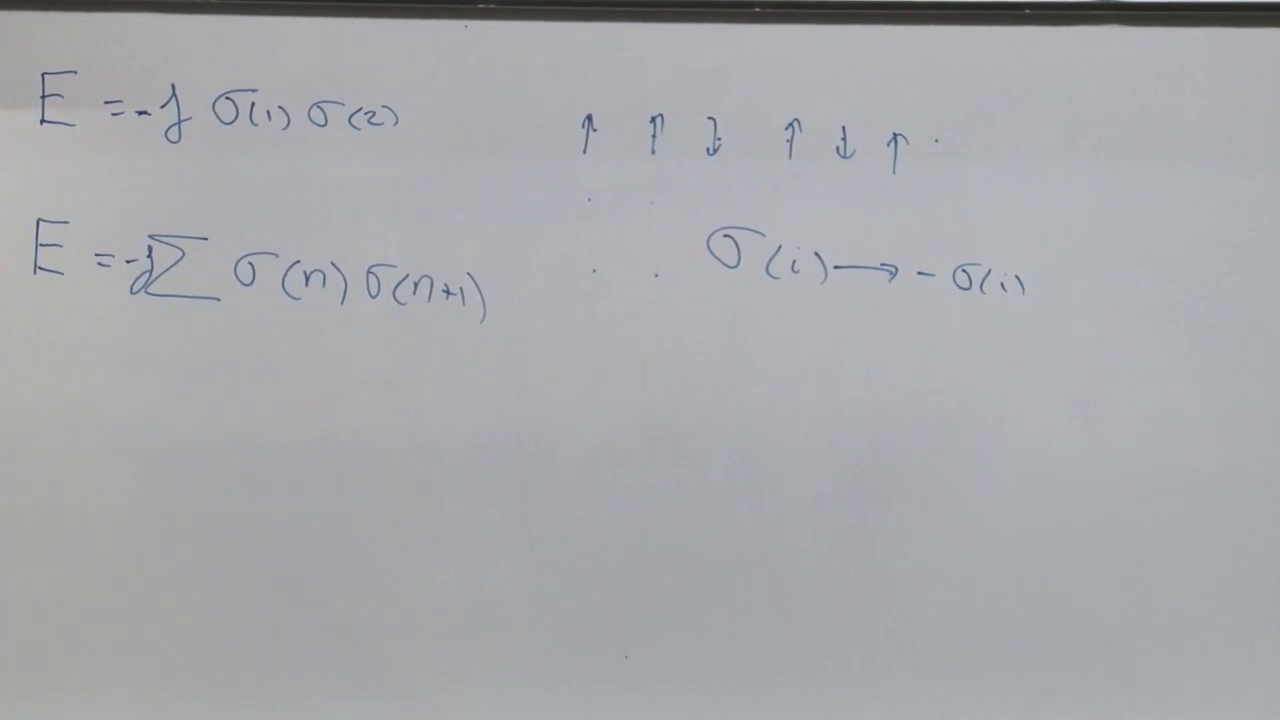
\includegraphics[width=0.90\textwidth]{lecture_08_figure_11.png}
\caption{链的哈密顿量与全局变换
\(\sigma_i\mapsto-\sigma_i\)并列，后者使每一对乘积保持不变。}
\lectureframe{01:26:31}
\end{figure}

在严格零温下对某一个自旋施加一个极微小的场。它打破两个基态之间的平局，而铁磁耦合将这一选择沿链传播开来。在态被选定之后撤去该场，一个大系统可以在极长的时间内保持其取向。这是通向自发对称性破缺的直观入口。

有一个本质性的统计限定。对于处于严格零场中的有限系统，正则系综给两个基态以相等的权重，因而平均磁化强度为零。破缺对称性的相是通过在撤去选择场之前先取热力学极限来定义的：
\begin{equation}
 M_*=\lim_{H\to0^+}\lim_{N\to\infty}M_N(H).
 \label{eq:sm8-order-of-limits}
\end{equation}
在一维最近邻模型中，这一极限仅在\(T=0\)处非零；任何有限温度都会破坏无限长链中的长程有序。在二维中，有序相在低于某个非零临界温度时仍然存在。

\subsection{一个历史性的更正}

课堂上的讲述在叙述这段历史时拿伊辛开了个玩笑。准确的年代顺序则更为友善。威廉·楞次提出了该模型，他的学生恩斯特·伊辛在其1924年的学位论文中求解了一维情形，该论文发表于1925年。伊辛正确地发现一维中不存在有限温度的鐵磁相变，尽管当时人们尚未理解更高维度的更广泛意义。克拉默斯与万尼尔发展了二维对偶性，并在1941年确定了方格点阵的临界点；昂萨格在1944年给出了著名的零场精确解。

接下来的计算现在已很明确。我们必须求出\eqref{eq:sm8-ising-chain-open}的配分函数，并确定其关联如何依赖于温度。该计算将明确显示为什么一维链没有有限温度相变，以及为什么维度至关重要。

\section{我们目前的进展}

回归问题与自旋问题是同一统计教训的两个版本。在气体中，熵的亏缺使一个宏观态以指数方式变得稀有：
\begin{equation}
 P(A)=e^{-\Delta S},
 \qquad
 \tau_{\rm rec}\sim\tau_{\rm mix}e^{\Delta S}.
 \label{eq:sm8-summary-recurrence}
\end{equation}
可逆力学允许回归，而巨大的相体积比解释了为什么日常经验只看到弛豫。剩下的时间箭头问题在于特殊的宇宙学初始条件，而不在于微观可逆性的失效。

对于场中的独立自旋，
\begin{equation}
 Z_N=\left[2\cosh(\beta\mu H)\right]^N,
 \qquad
 M=-\tanh(\beta\mu H).
 \label{eq:sm8-summary-spins}
\end{equation}
该系统明显是有偏置的，并随温度平滑变化。伊辛相互作用
\begin{equation}
 {\cal H}=-J\sum_i\sigma_i\sigma_{i+1}
 \label{eq:sm8-summary-ising}
\end{equation}
去除了外部偏置，恢复了全局上--下对称性，并提出了真正的有序化问题：一个对称的多体系统能否在非零温度下选择两个有序态之一？

\chapter{伊辛关联、平均场与自发磁化}

\lectureoverview{一维伊辛链可以通过将格点自旋替换为键变量来精确求解。这一变量替换把配分函数变成一个乘积，并表明所有有限温度下的关联都按指数衰减。高维点阵的行为则不同，因为每个自旋都从许多近邻接收信息。把它们的联合影响当作一个平均场来处理，就得到一个自洽方程、一个平均场临界温度，以及关于任意小的外场如何选定一个磁化相的精确说明。}

\section{伊辛实际发现了什么}

历史要点应当准确陈述。恩斯特·伊辛求解了威廉·楞次交给他的一维模型，并正确地发现不存在有限温度相变。过分之处在于推断同一结论应当在所有维度都成立。事实并非如此。二维模型已经具有有序的低温相。

高维的精确解对于当前目的来说过于雄心勃勃。一个物理上透明的近似就足以在每个自旋有许多近邻时揭示相变。然而，在作此近似之前，值得先精确求解一维链。精确的一维答案与高维近似之间的对比，指出了维数为一时所缺少的机制。

这里的相变不只是已有偏好逐渐增强。当温度越过一个临界值时，平衡态获得了一种新的宏观性质：即使用来使样品取向的外场已被撤去，非零磁化仍能持续存在。因此，计算必须回答两个彼此独立的问题。一个远处的自旋是否记得某个选定自旋的取向，以及一个无穷小的场能否组织起任意大的样品？

\section{单个自旋作为可复用的构建单元}

取一个二态变量
\begin{equation}
\sigma=\pm1,
\end{equation}
并选择能量约定
\begin{equation}
E(\sigma)=-J\sigma,
\qquad J>0.
\end{equation}
于是态\(\sigma=+1\)具有较低的能量。参数\(J\)可以代表磁矩乘以外加场，但在此计算中只有其乘积进入。

把这个自旋看作与其余一切处于热平衡的小子系统。其配分函数为
\begin{align}
z
&=\sum_{\sigma=\pm1}e^{-\beta E(\sigma)}
 =\sum_{\sigma=\pm1}e^{\beta J\sigma} \\
&=e^{\beta J}+e^{-\beta J}
 =2\cosh(\beta J).
\end{align}

同一结果也可以嵌入到\(N\)个独立自旋的集合中。完整配分函数将简单地是\(Z=z^N\)，因此\(\log Z=N\log z\)，而每个广延热力学量都将是其单自旋值的\(N\)倍。这种子系统观点取代了关于有多少自旋朝上、多少朝下的较长组合计数，但它包含同样的信息。
平均能量由对数导数给出：
\begin{align}
\expect{E}
&=-\frac{\partial}{\partial\beta}\log z \\
&=-J\frac{\sinh(\beta J)}{\cosh(\beta J)}
 =-J\tanh(\beta J).
\end{align}
由于\(E=-J\sigma\)，
\begin{equation}
\expect{\sigma}=\tanh(\beta J).
\end{equation}

\begin{figure}[ht]
\centering
\includegraphics[width=0.80\textwidth]{lecture_09_figure_02.png}
\caption{化为双曲正切形式的单自旋能量与磁化。}
\lectureframe{00:10:06}
\end{figure}

这一个公式包含了两个温度极限。在低温下，\(\beta J\gg1\)，自旋几乎必然处于较低能量的态。在高温下，\(\beta J\ll1\)，所以
\begin{equation}
\expect{\sigma}\simeq \beta J\longrightarrow0.
\end{equation}
热骚动抹去了能量偏好。

\begin{classroomqa}
\audiencequestion{平均能量应当带负号吗？}
\lecturerresponse{是的。热力学恒等式是\(\expect{E}=-\partial_\beta\log z\)，所以结果是\(-J\tanh(\beta J)\)。再除以\(E=-J\sigma\)中的因子\(-J\)，就得到正的磁化\(\expect{\sigma}=\tanh(\beta J)\)。\lecturetimestamp{00:09:15--00:09:44}}
\end{classroomqa}

\section{一维链}

把\(N\)个自旋放在一条开链上，并让相邻自旋相互作用：
\begin{equation}
H=-J\sum_{i=1}^{N-1}\sigma_i\sigma_{i+1},
\qquad \sigma_i=\pm1.
\label{eq:ising-chain}
\end{equation}
对于\(J>0\)，平行的一对贡献\(-J\)，而反平行的一对贡献\(+J\)。因此两个基态是
\begin{equation}
(+,+,\ldots,+)
\qquad\text{and}\qquad
(-,-,\ldots,-).
\end{equation}

\begin{figure}[ht]
\centering
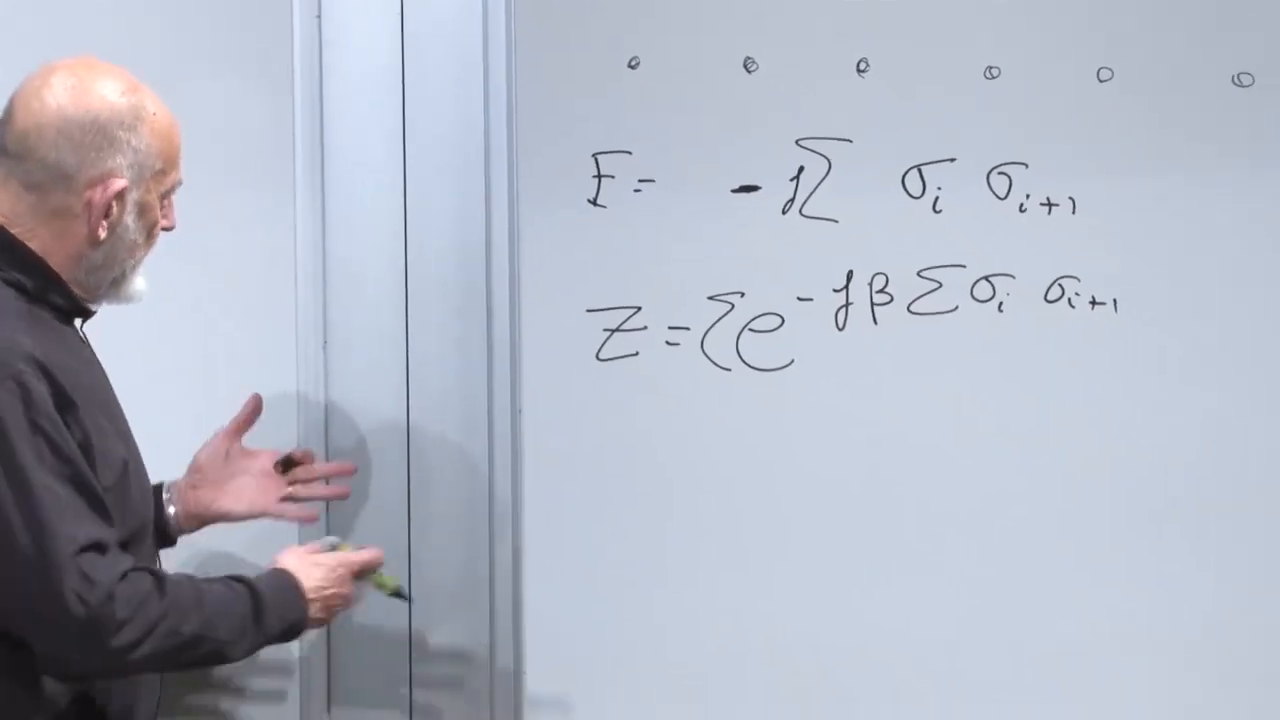
\includegraphics[width=0.80\textwidth]{lecture_09_figure_03.png}
\caption{开链哈密顿量及其玻尔兹曼求和。}
\lectureframe{00:19:15}
\end{figure}

把\(J\)改为\(-J\)会偏好交替自旋。在开链上，或在偶数周期链上，重新定义
\begin{equation}
\widetilde{\sigma}_i=(-1)^i\sigma_i
\end{equation}
把反铁磁符号映射回铁磁符号。这一区别是物理的，但一维配分函数的代数运算相同。奇数周期链是熟悉的例外，因为它无法在不产生阻挫的情况下交替。

\begin{classroomqa}
\audiencequestion{链的哈密顿量中有外磁场吗？}
\lecturerresponse{还没有。式~\eqref{eq:ising-chain}只包含最近邻耦合。均匀外场稍后将作为一个单独的项\(-h\sum_i\sigma_i\)加入，正是为了检验有序态如何响应任意小的偏置。\lecturetimestamp{00:18:54--00:19:13}}
\end{classroomqa}

\subsection{作为关联函数的记忆}

假设已知\(\sigma_i\)处于向上态。这一信息是否会影响相隔\(r\)个键的自旋？诊断量为
\begin{equation}
C(r)=\expect{\sigma_i\sigma_{i+r}}.
\end{equation}
若当\(r\to\infty\)时\(C(r)\)趋于一个非零数，则系统保留长程记忆。若它趋于零，则第一个自旋的影响最终消失。

传话游戏给出了正确的直觉。每个人向下一个人传递一个二进制符号。若每次传递都完美无误，初始比特将无限期地存留下去。若每一步都有任何非零的错误概率，反复传递最终会丢失原始信息。零温度是伊辛链的完美传递极限。任何正温度都允许相邻自旋之间偶尔出现不一致。

为了给出一个数值图像，假设单次传递的保真度为\(0.99\)。两次完美传递发生的概率为\(0.99^2=0.9801\)，而每增加一步就再提供一个因子\(0.99\)。一百步就已经使错误变得常见；一万步则抹去实际意义上的记忆。伊辛链使用的是保真度的带符号度量，而非这种无错误概率，但乘性损失是同样的思想。

在区分概率与关联之后，这个类比就变得精确了。若\(p\)是相邻自旋一致的概率，则
\begin{equation}
\expect{\sigma_i\sigma_{i+1}}
=p-(1-p)=2p-1.
\end{equation}
因此，逐键相乘的量是超额保真度\(2p-1\)，而不是\(p\)本身。

\section{键变量与精确配分函数}

决定性的变量替换是描述关系而非单个自旋：
\begin{equation}
\mu_i=\sigma_i\sigma_{i+1},
\qquad i=1,\ldots,N-1.
\label{eq:bond-variable}
\end{equation}
每个键变量在一致时为\(+1\)，在不一致时为\(-1\)。若固定第一个自旋，则这些键决定之后每一个自旋：
\begin{align}
\sigma_2&=\sigma_1\mu_1,\\
\sigma_3&=\sigma_1\mu_1\mu_2,\\
\sigma_{r+1}&=\sigma_1\prod_{k=1}^{r}\mu_k.
\end{align}
这里没有冗余。数据\((\sigma_1,\mu_1,\ldots,\mu_{N-1})\)等价于\((\sigma_1,\ldots,\sigma_N)\)。

在这些变量下，能量简单地成为
\begin{equation}
H=-J\sum_{i=1}^{N-1}\mu_i.
\end{equation}
原本相互作用的格点变量已变成相互独立的键变量。先对\(\sigma_1\)的两个取值求和，得到
\begin{align}
Z_N
&=2\sum_{\{\mu_i=\pm1\}}
\exp\left(\beta J\sum_{i=1}^{N-1}\mu_i\right)\\
&=2\prod_{i=1}^{N-1}
\left(\sum_{\mu_i=\pm1}e^{\beta J\mu_i}\right)\\
&=2\left[2\cosh(\beta J)\right]^{N-1}.
\label{eq:chain-partition}
\end{align}
共有\(N-1\)个因子，因为含\(N\)个格点的开链有\(N-1\)个键。

前面的因子二来自第一个自旋的全局选择。它对\(\log Z_N\)只贡献\(\log2\)，而键则贡献一个正比于\(N-1\)的项。该因子对于精确的有限尺寸计数很重要，但当\(N\to\infty\)时它从自由能密度中消失。这就是为什么板书可以说它“没什么大不了”，而实际上并没有把它丢弃。

\begin{figure}[ht]
\centering
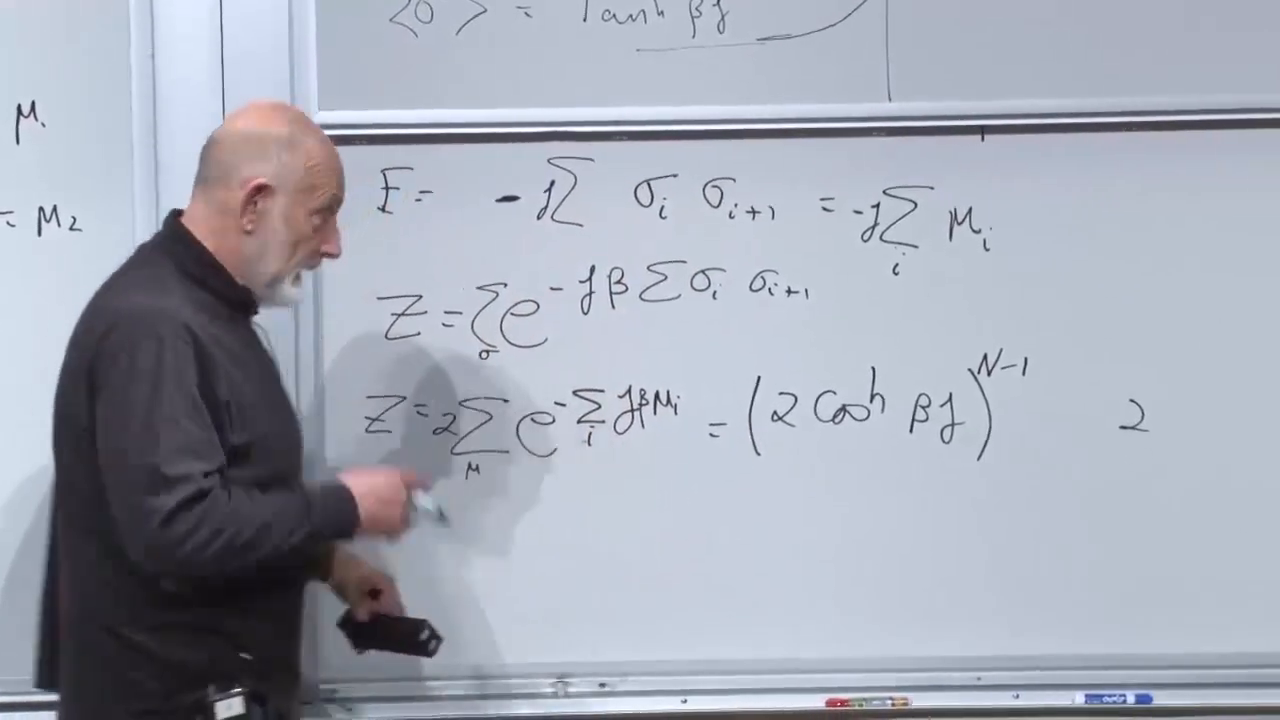
\includegraphics[width=0.82\textwidth]{lecture_09_figure_04.png}
\caption{将格点哈密顿量改写为对独立键的求和，以及由此得到的因子化配分函数。}
\lectureframe{00:35:35}
\end{figure}

\begin{classroomqa}
\audiencequestion{当最终答案变成幂时，指数中的求和到哪里去了？}
\lecturerresponse{它在变成幂之前先变成了乘积：
\[
e^{\beta J\sum_i\mu_i}=\prod_i e^{\beta J\mu_i}.
\]
对所有键构型的求和随后分解为每个键的一个两项求和。由于每个因子都是\(2\cosh(\beta J)\)，乘积就是它的\((N-1)\)次幂。写出三个自旋和两个键的情形，可以使因子化完全明确。\lecturetimestamp{00:33:25--00:35:36}}
\end{classroomqa}

这是一个简单的对偶描述：格点上的耦合变量已被替换为键上的非耦合变量。\emph{对偶}一词是恰当的，因为同一系统具有两种自由度看起来非常不同的描述。在这里，它是针对一维开链的一个精确变量替换。

用点阵的语言来说，原始变量生活在顶点上，而新变量生活在边上。第一个自旋的全局选择是从边重构顶点所需的唯一额外数据。这种格点—键的交换是这样一个模式的一个朴素例子，而该模式在高维统计力学中会变得强大得多。

\subsection{最近邻保真度}

每个键都有相同的分布，
\begin{equation}
\begin{aligned}
\Pr(\mu=+1)&=\frac{e^{\beta J}}{2\cosh(\beta J)},\\
\Pr(\mu=-1)&=\frac{e^{-\beta J}}{2\cosh(\beta J)}.
\end{aligned}
\end{equation}
因此，
\begin{equation}
\expect{\mu_i}
=\expect{\sigma_i\sigma_{i+1}}
=\tanh(\beta J).
\label{eq:nearest-correlation}
\end{equation}

\begin{figure}[ht]
\centering
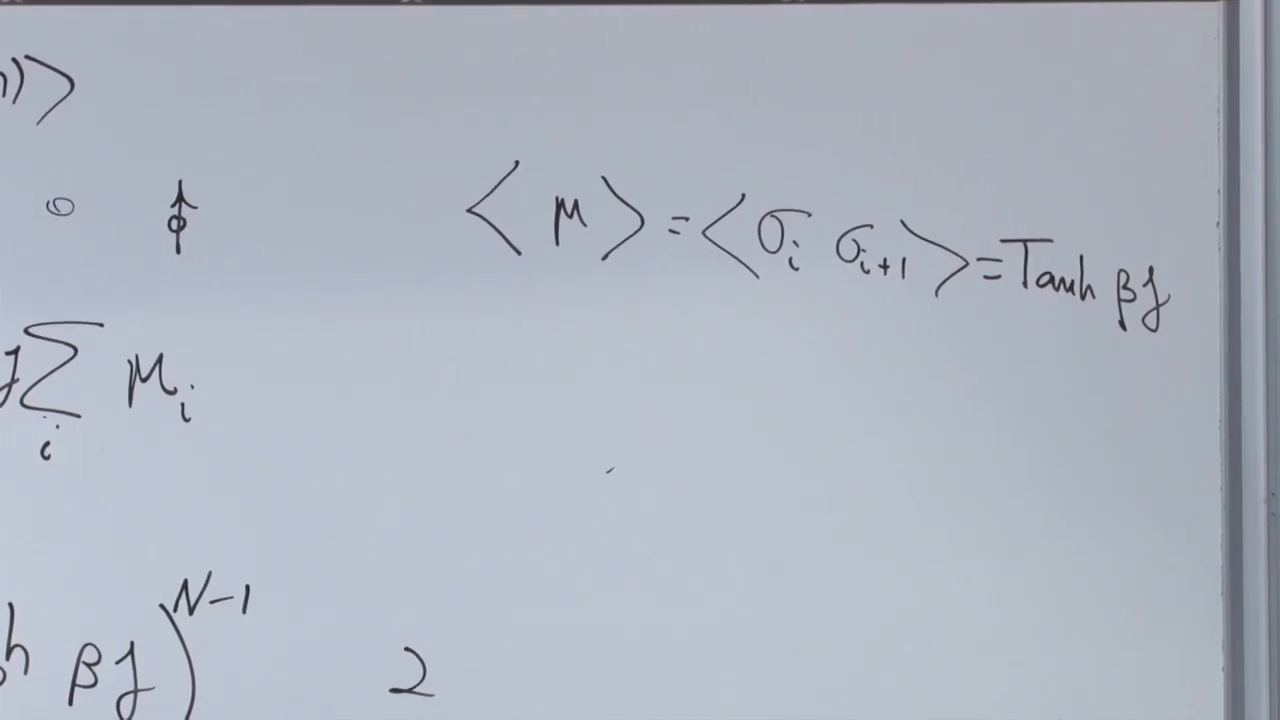
\includegraphics[width=0.80\textwidth]{lecture_09_figure_05.png}
\caption{将最近邻关联表示为键变量的平均值。}
\lectureframe{00:36:52}
\end{figure}

因此，相邻自旋一致的概率为
\begin{equation}
p_{\rm same}
=\frac{1+\tanh(\beta J)}{2}.
\end{equation}
它在正\(J\)时超过二分之一，在零温度时趋于一，而在无穷大温度时变为二分之一。

\begin{classroomqa}
\audiencequestion{为什么正的最近邻关联意味着自旋倾向于同向排列而不是反向排列？}
\lecturerresponse{对于\(J>0\)，同向键的能量为\(-J\)，反向键的能量为\(+J\)。\(\expect{\mu}\)为正值说明\(\mu=+1\)，即同向排列，出现得更频繁。真实材料究竟具有铁磁还是反铁磁的有效耦合，取决于其微观电子结构；这里的符号约定描述的是铁磁体。\lecturetimestamp{00:43:45--00:44:48}}
\end{classroomqa}

\begin{classroomqa}
\audiencequestion{在非常高的温度下，这个关联会怎样？}
\lecturerresponse{当\(T\to\infty\)时，\(\beta\to0\)，且\(\tanh(\beta J)\to0\)。此时即使最近邻之间也不携带关于彼此的任何信息：每个自旋实际上都是随机猜测。\lecturetimestamp{00:46:42--00:47:20}}
\end{classroomqa}

\subsection{长程关联}

对于相隔\(r\)个键的自旋，
\begin{align}
\sigma_i\sigma_{i+r}
&=\sigma_i
\left(\prod_{k=i+1}^{i+r-1}\sigma_k^2\right)
\sigma_{i+r}\\
&=(\sigma_i\sigma_{i+1})
(\sigma_{i+1}\sigma_{i+2})\cdots
(\sigma_{i+r-1}\sigma_{i+r})\\
&=\prod_{k=i}^{i+r-1}\mu_k.
\end{align}
由于\(\mu_k\)相互独立，
\begin{equation}
C(r)=\expect{\sigma_i\sigma_{i+r}}
=\left[\tanh(\beta J)\right]^r.
\label{eq:exact-correlation}
\end{equation}

\begin{figure}[ht]
\centering
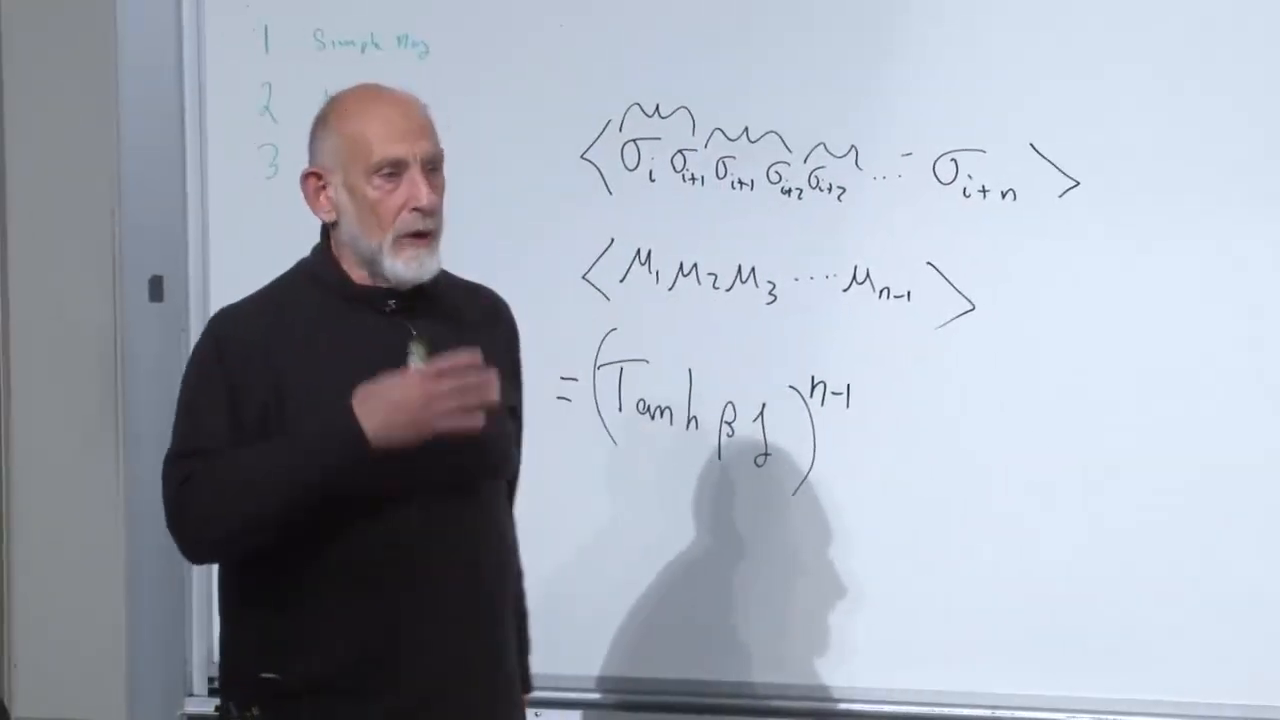
\includegraphics[width=0.80\textwidth]{lecture_09_figure_06.png}
\caption{中间的\(\sigma_k^2=1\)因子将远端自旋的乘积转化为独立键的乘积。}
\lectureframe{00:41:35}
\end{figure}

\begin{classroomqa}
\audiencequestion{关联函数只包含两个端点自旋。那么所有中间自旋是从哪里来的？}
\lecturerresponse{它们只是作为等于1的因子被插入：\(\sigma_k^2=1\)。将相邻的副本配对，就把端点乘积转化为键变量，而这些正是其热分布可因式分解的变量。关联函数的值并未改变。\lecturetimestamp{00:41:41--00:42:26}}
\end{classroomqa}

在任意有限温度下，
\begin{equation}
0<\tanh(\beta J)<1,
\end{equation}
因此记忆呈指数衰减。写出
\begin{equation}
C(r)=e^{-r/\xi}
\end{equation}
即定义了精确的关联长度
\begin{equation}
\xi^{-1}=-\log\!\left[\tanh(\beta J)\right].
\label{eq:correlation-length}
\end{equation}
只有在\(T=0\)时，\(\xi\)才发散。在低但非零的温度下，
\begin{equation}
\xi\simeq \frac{1}{2}e^{2\beta J},
\end{equation}
因此链中可以包含非常长的同向排列段，却不具有真正的无限程有序。

因此这条链看起来是成团的。人们看到一长串自旋向上，然后一次翻转，接着一长串自旋向下，然后再一次翻转。低温使这些串变长，因为畴壁很稀少；它并不会完全消除畴壁。磁化需要无限长的记忆长度，而不仅仅是很大的记忆长度。

\section{为什么更多邻居会改变问题}

一维不提供任何纠错能力。一旦某个键与其前驱不一致，下一个自旋就没有独立的信息来源告诉它原本意图是哪个取向。因此这条链由被偶尔翻转隔开的长同向排列畴组成。

在正方点阵中，每个格点有四个最近邻。在立方点阵中，它有六个。在\(d\)维超立方点阵中，它有
\begin{equation}
z=2d
\end{equation}
个最近邻。一个格点若收到三条一致的信息和一条不一致的信息，就可以遵从多数。多邻居环境抑制孤立错误的方式，与冗余信息实现纠错的方式大致相同。

如果邻居的平均自旋为\(m\)，则它们的和具有平均值\(zm\)。其普通涨落量级为\(\sqrt{z}\)，因此在远离\(m=0\)处，相对涨落大致按如下方式标度：
\begin{equation}
\frac{\sqrt{z}}{z|m|}
=\frac{1}{\sqrt{z}\,|m|}.
\end{equation}
这就是为什么在大的配位数下平均场变得可信。它也提醒我们，在临界点附近\(m\)很小，该近似最不可靠。

一句被记住的谚语抓住了大数直觉：一百张独立的选票不太可能全都朝同一方向出错。其定量版本就是平方根定律。\(z\)个变量中的相干偏置正比于\(z\)，而随机不一致通常只正比于\(\sqrt{z}\)。因此，增大维度不仅改变邻居的数量，也改变它们集体信息的可靠性。

\begin{classroomqa}
\audiencequestion{高于三维的维度是否对应某种物理磁性材料？}
\lecturerresponse{不能直接作为空间维度来对应。大的\(d\)是一个可解极限，其中每个格点有许多邻居，平均化变得可控。一旦在那里看清了机制，就可以追问它在多大程度上能延续到物理维度。对于Ising模型，二维已经足以出现有限温度相变，尽管平均场并不能给出精确的二维答案。\lecturetimestamp{00:52:32--00:53:50}}
\end{classroomqa}

\section{作为自洽问题的平均场}

聚焦于一个自旋\(\sigma_i\)。它与它的\(z=2d\)个邻居的相互作用为
\begin{equation}
E_i=-J\sigma_i\sum_{j\in{\rm nn}(i)}\sigma_j.
\label{eq:local-energy}
\end{equation}
令
\begin{equation}
m=\expect{\sigma}
\end{equation}
表示每个自旋的均匀磁化。平均场将涨落的邻居和替换为其平均值：
\begin{equation}
\sum_{j\in{\rm nn}(i)}\sigma_j
\longrightarrow zm=2dm.
\end{equation}
于是这个被选定的自旋具有有效的单自旋能量
\begin{equation}
E_i^{\rm MF}=-2dJm\,\sigma_i.
\label{eq:mean-field-energy}
\end{equation}

\begin{figure}[ht]
\centering
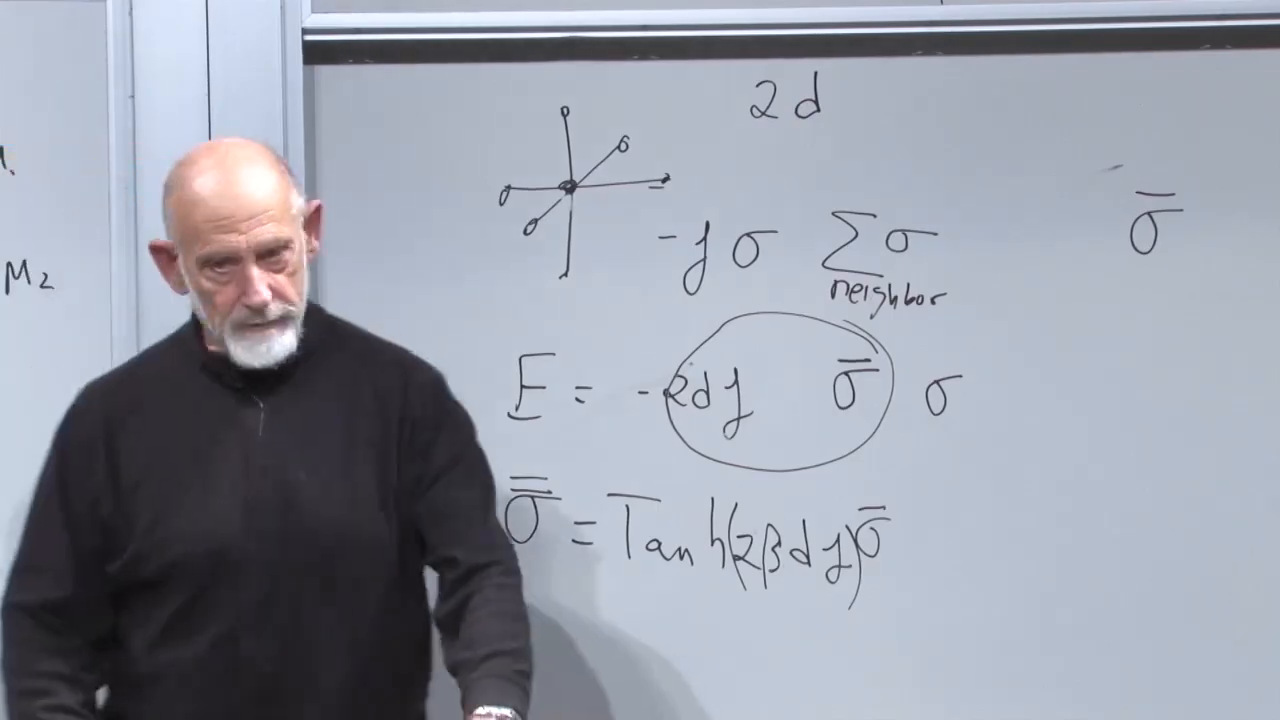
\includegraphics[width=0.82\textwidth]{lecture_09_figure_07.png}
\caption{一个选定的自旋、它的\(2d\)个最近邻，以及用平均磁化强度替换它们的和。}
\lectureframe{01:00:30}
\end{figure}

现在可以用有效场\(2dJm\)重新使用单自旋的结果：
\begin{equation}
\expect{\sigma_i}_{\rm effective}
=\tanh(2\beta dJm).
\end{equation}
但所选格点并不特殊。平移不变性要求它的平均值等于所假设的平均值\(m\)。因此
\begin{equation}
\boxed{m=\tanh(2\beta dJm)}.
\label{eq:self-consistency}
\end{equation}
这就是为什么平均场也称为自洽场近似：产生有效场的磁化强度必须等于由该场产生的磁化强度。

\begin{classroomqa}
\audiencequestion{有效单自旋答案中是否缺少一个\(\beta\)因子？}
\lecturerresponse{它必须存在。指数或双曲正切的宗量是无量纲的，因此有效能量\(2dJm\)表现为\(2\beta dJm\)。\lecturetimestamp{01:00:13--01:00:27}}
\end{classroomqa}

\begin{classroomqa}
\audiencequestion{这个方程只是说\(m\)与自身成正比吗？}
\lecturerresponse{不是。未知的磁化强度出现在一个非线性函数内部：
\[
m=\tanh(2\beta dJm).
\]
这是一个隐式方程，可能有一个或几个解，取决于温度。\lecturetimestamp{01:02:12--01:02:42}}
\end{classroomqa}

\begin{classroomqa}
\audiencequestion{自洽方程是否假设高温或双曲正切的宗量很小？}
\lecturerresponse{不是。方程\(m=\tanh(2\beta dJm)\)是在每个温度下的完整平均场方程。只有像\(\tanh x\simeq x\)这样的后续近似才要求\(x\)很小，它被用于临界点附近以确定或展开新出现的解。\lecturetimestamp{01:02:44--01:03:12}}
\end{classroomqa}

\begin{classroomqa}
\audiencequestion{上划线记号与通常的尖括号平均不同吗？}
\lecturerresponse{不。黑板上使用的横线是热平均的简写：\(\bar{\sigma}=\expect{\sigma}=m\)。\lecturetimestamp{01:03:19--01:03:42}}
\end{classroomqa}

\begin{classroomqa}
\audiencequestion{这\(2d\)个自旋都是最近邻吗，更长程的耦合会有类似的效果吗？}
\lecturerresponse{在超立方点阵上，是的：沿\(d\)个坐标轴中的每一个都有两个最近邻。次近邻和更远距离的耦合是另一个模型，通常带有它们自己的强度，但增加相互作用范围也会提高有效配位数，并能使平均场推理更准确。\lecturetimestamp{01:03:43--01:05:12}}
\end{classroomqa}

\section{相变的图示}

定义
\begin{equation}
K=2\beta dJ,
\qquad
y=Km.
\end{equation}
则方程~\eqref{eq:self-consistency}变为
\begin{equation}
\frac{y}{K}=\tanh y.
\label{eq:graph-equation}
\end{equation}
右边是一个固定的S形函数。左边是一条过原点、斜率为
\begin{equation}
\frac{1}{K}=\frac{T}{2dJ},
\end{equation}
的直线，其中\(k_{\rm B}=1\)。

在高温下，这条直线很陡，只与\(\tanh y\)相交于\(y=0\)。在低温下，这条直线较平缓，有三个交点：\(y=0\)和一对对称的\(y=\pm y_0\)。阈值出现在直线与\(\tanh y\)在原点处斜率相同时。由于\(\tanh'(0)=1\)，
\begin{equation}
K_c=1,
\qquad
T_c^{\rm MF}=2dJ.
\label{eq:mean-field-tc}
\end{equation}
这是平均场临界温度，而不是低维中的精确答案。

假设\(J>0\)说明相邻自旋倾向于一致；它并不在\(+m\)与\(-m\)之间做出选择。在零外场下，哈密顿量在全局翻转\(\sigma_i\mapsto-\sigma_i\)下不变，因此两个非零交点在物理上等价。只取图的右半部分是一种方便的绘图约定，而不是丢失了负相。

\begin{figure}[ht]
\centering
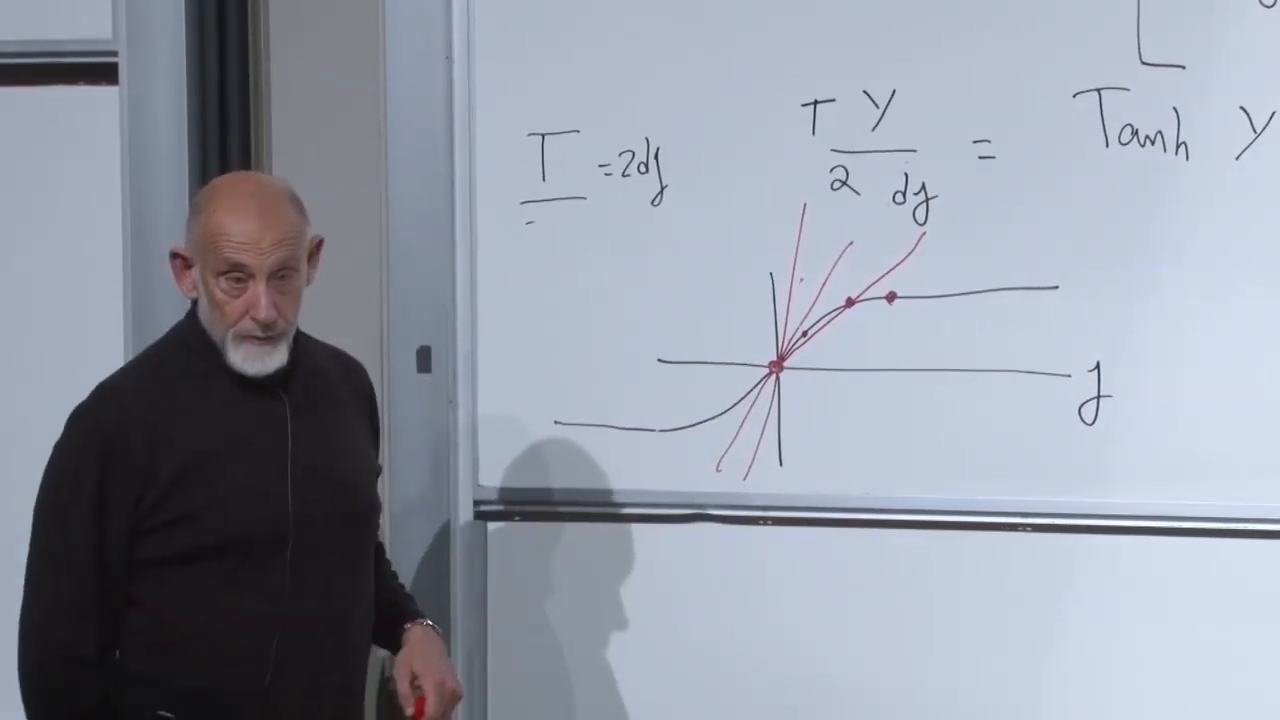
\includegraphics[width=0.82\textwidth]{lecture_09_figure_08.png}
\caption{直线族与\(\tanh y\)：一个高温交点与三个低温交点。}
\lectureframe{01:11:50}
\end{figure}

\begin{figure}[ht]
\centering
\begin{tikzpicture}[x=1.15cm,y=2.0cm]
\draw[->] (-3.2,0) -- (3.2,0) node[right] {$y$};
\draw[->] (0,-1.15) -- (0,1.15);
\draw[thick,blue!70!black,domain=-3:3,samples=120]
  plot (\x,{tanh(\x)}) node[right] {$\tanh y$};
\draw[thick,red!70!black] (-0.85,-1.15) -- (0.85,1.15)
  node[pos=0.70,left] {high \(T\)};
\draw[thick,orange!85!black] (-1.15,-1.15) -- (1.15,1.15)
  node[pos=0.86,right] {\(T_c^{\rm MF}\)};
\draw[thick,green!45!black] (-3,-0.72) -- (3,0.72)
  node[right] {low \(T\)};
\fill (0,0) circle (1.4pt);
\fill[green!45!black] (-2.45,-0.588) circle (1.5pt);
\fill[green!45!black] (2.45,0.588) circle (1.5pt);
\end{tikzpicture}
\caption{对图解法自洽论证的归一化重构。}
\end{figure}

非零分支连续地出现。在转变附近，
\begin{equation}
\tanh(Km)=Km-\frac{(Km)^3}{3}+O(m^5).
\end{equation}
对于\(K>1\)，小的非零解满足
\begin{equation}
m^2\simeq \frac{3(K-1)}{K^3}.
\end{equation}
因此平均场预言了熟悉的平方根式起始\(m\propto(T_c-T)^{1/2}\)。

稳定性陈述也可以不依赖于图的画法来给出。在相差一个与\(m\)无关的常数的意义下，每自旋的平均场自由能为
\begin{equation}
f_{\rm MF}(m)
=dJm^2-\frac{1}{\beta}
\log\!\left[2\cosh(2\beta dJm)\right].
\label{eq:mf-free-energy}
\end{equation}
其驻定条件为
\begin{equation}
\frac{\partial f_{\rm MF}}{\partial m}
=2dJ\left[m-\tanh(2\beta dJm)\right]=0.
\end{equation}
在\(T_c^{\rm MF}\)以上，\(m=0\)是最小值。在其以下，原点是局部极大值，而两个非零解是简并的最小值。交点的几何与自由能的热力学说的是同一件事。

\begin{classroomqa}
\audiencequestion{解\(m=0\)在\(T_c^{\rm MF}\)以下仍是一个交点。为什么非零分支应当是物理的？}
\lecturerresponse{从零温开始将系统向上移动，已经把它置于一个磁化分支上。更形式化地说，在转变温度以下，平均场自由能在\(\pm m_0\)处有极小值，而\(m=0\)则成为极大值。于是无穷小的外场会选中一个极小值，并消除表面上的歧义。\lecturetimestamp{01:11:34--01:12:18}}
\end{classroomqa}

\section{为什么一维会击败平均场}

将\(d=1\)代入方程~\eqref{eq:mean-field-tc}会预言在\(T=2J\)处发生转变，这与精确的一维解相矛盾。并没有任何代数量发散。该近似之所以失败，是因为两个近邻并不构成一个大的统计热浴，也因为一维畴壁带有异常的熵。

从全向上的态出发。一个断键将其能量从\(-J\)变为\(+J\)，因此每个断键的代价为
\begin{equation}
\Delta E_{\rm bond}=2J.
\end{equation}
在正方点阵上，一个翻转的自旋断开四个键，代价为\(8J\)。两个相邻的翻转自旋具有六个断键的周长，代价为\(12J\)，而两个相距很远的翻转则断开八个键，代价为\(16J\)。

\begin{figure}[ht]
\centering
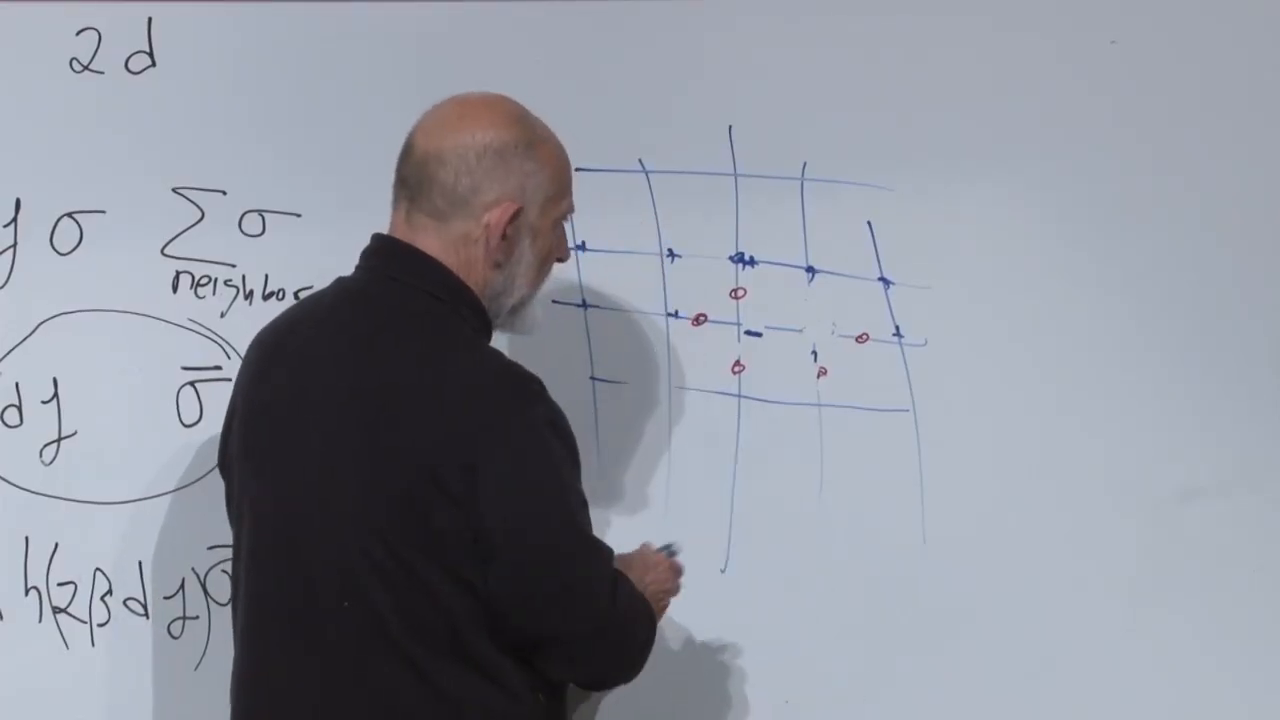
\includegraphics[width=0.82\textwidth]{lecture_09_figure_09.png}
\caption{正方点阵中两个相邻的反向自旋；它们共享的键得到满足，留下六键边界。}
\lectureframe{01:17:30}
\end{figure}

因此在二维中，一个紧凑的反向液滴所付出的能量正比于其边界长度：
\begin{equation}
\Delta E_{\rm 2d}=2J\,|\partial D|.
\end{equation}
使液滴长大通常也会使其边界长大。

一维则不同。一个连续的反向块，无论多长，都只有两个畴壁：
\begin{equation}
\Delta E_{\rm 1d}=2(2J)=4J.
\label{eq:one-d-domain-cost}
\end{equation}

\begin{figure}[ht]
\centering
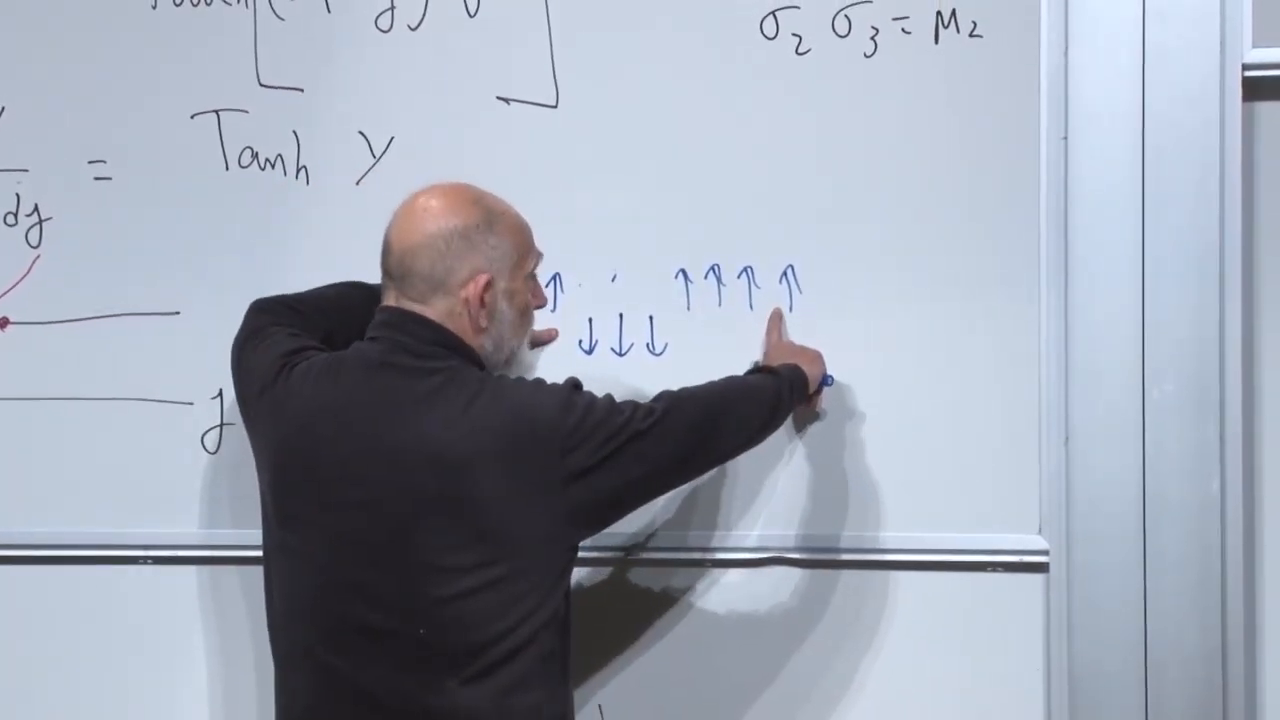
\includegraphics[width=0.82\textwidth]{lecture_09_figure_10.png}
\caption{一维中一个长反向块仅由两个畴壁界定。}
\lectureframe{01:19:10}
\end{figure}

在一条有\(N\)个格点的链中，选择这样一个块的两个壁的方式有\(N^2\)量级种。它们的能量并不随两壁之间间距的增大而增大。因此在任何正温度下，熵都会提供任意大的反向畴。在二维中，边界能量在足够低的温度下可以战胜轮廓熵。这种能量—熵竞争正是平均场在把\(d=1\)和\(d=2\)仅仅当作同一系数的不同数值处理时所看不到的几何事实。

\begin{classroomqa}
\audiencequestion{恒定的双壁代价是否要求翻转的自旋彼此相邻？}
\lecturerresponse{是的。该论断针对的是一个连续的反向块。如果翻转的自旋形成若干个分离的块，那么每个块都会引入两个额外的畴壁。要点在于，单个块可以任意长，却仍然只保留两个壁。\lecturetimestamp{01:18:32--01:18:40}}
\end{classroomqa}

\begin{classroomqa}
\audiencequestion{平均场方程本身似乎并未显示出\(d=1\)与\(d=2\)之间的定性区别。问题就在这里吗？}
\lecturerresponse{正是如此。平均场对每一个正的\(d\)都预言存在转变，因此它在一维中是定性错误的。它的推导假定了许多弱涨落的近邻，并丢弃了畴壁几何。决定一维情形的是精确的键解，而不是平均场替换\(d=1\)。\lecturetimestamp{01:19:44--01:20:28}}
\end{classroomqa}

\section{外场选择相}

加入一个均匀场\(h\)，约定\(h>0\)有利于\(\sigma=+1\)：
\begin{equation}
H=-J\sum_{\langle ij\rangle}\sigma_i\sigma_j
-h\sum_i\sigma_i.
\label{eq:ising-with-field}
\end{equation}
一个选定自旋的平均场能量为
\begin{equation}
E_i^{\rm MF}=-(2dJm+h)\sigma_i,
\end{equation}
而自洽方程变为
\begin{equation}
\boxed{m=\tanh\!\left[\beta(2dJm+h)\right]}.
\label{eq:self-consistency-field}
\end{equation}
取\(K=2\beta dJ\)和\(y=Km\)，
\begin{equation}
\frac{y}{K}=\tanh(y+\beta h).
\label{eq:shifted-graph}
\end{equation}

\begin{figure}[ht]
\centering
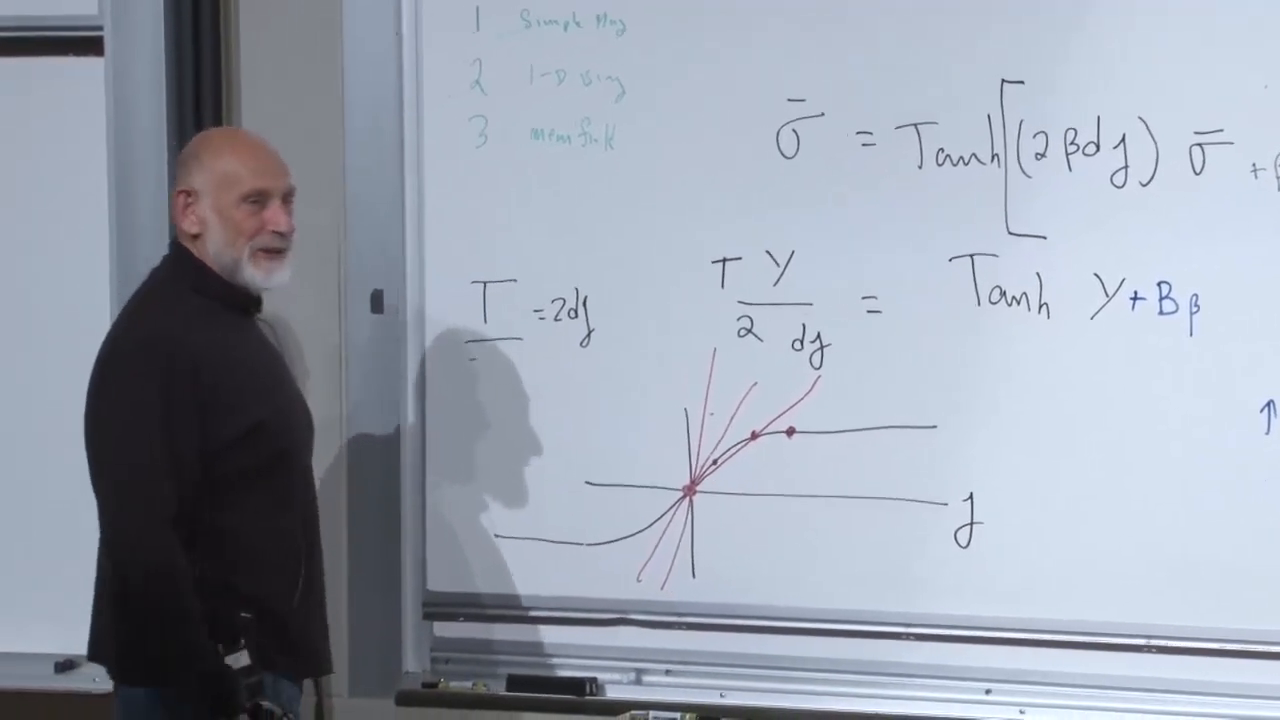
\includegraphics[width=0.82\textwidth]{lecture_09_figure_11.png}
\caption{在自洽方程中加入的外场项，以及相应的平移后图解构造。}
\lectureframe{01:26:20}
\end{figure}

\begin{classroomqa}
\audiencequestion{为什么场只加在双曲正切内部？它是否也应当改变左边？}
\lecturerresponse{左边是假定的磁化强度\(m\)，或等价地\(y/K\)。右边是在总有效场\(2dJm+h\)中为一个自旋计算出的磁化强度。自洽性令这两个量相等。将\(y=Km\)作为定义保持不变，就把新项只放进了自变量\(\tanh(y+\beta h)\)中。\lecturetimestamp{01:23:46--01:26:18}}
\end{classroomqa}

\begin{classroomqa}
\audiencequestion{同样的图解变化能否通过移动直线而不是平移\(\tanh\)曲线来描述？}
\lecturerresponse{可以。人们可以保持\(\tanh y\)不变，并改写方程，使直线具有非零截距。交点完全相同。这两种描述的区别仅在于选择方程哪一边作为固定图形。\lecturetimestamp{01:35:07--01:36:26}}
\end{classroomqa}

对于\(h\neq0\)，原点不再是解。在\(T_c^{\rm MF}\)以下，任意小的正场选择正分支；负场选择负分支。

\begin{figure}[ht]
\centering
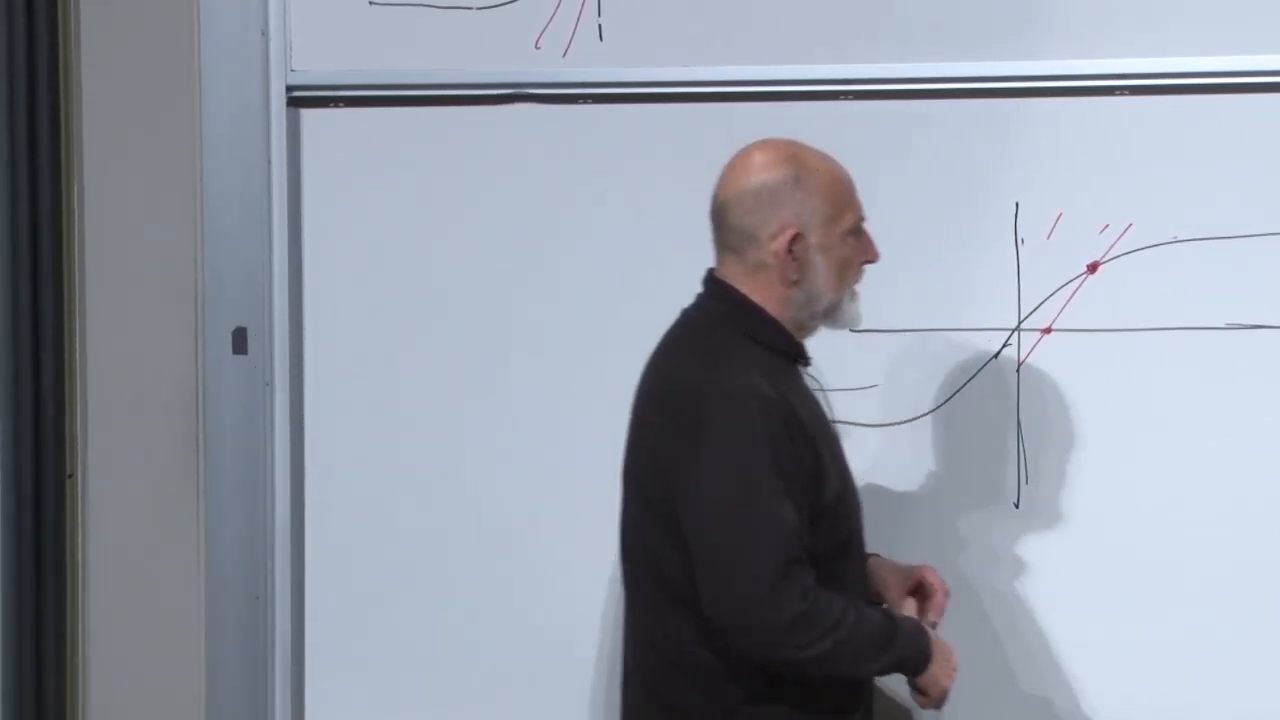
\includegraphics[width=0.82\textwidth]{lecture_09_figure_12.png}
\caption{弱场消除对称交点并选择一个磁化分支。}
\lectureframe{01:36:22}
\end{figure}

正确的陈述需要一个极限顺序。恰好处于\(h=0\)的有限系统具有自旋翻转对称性，因此在完整平衡系综中\(\expect{m}=0\)。自发磁化为
\begin{equation}
m_{\rm sp}
=\lim_{h\to0^+}\lim_{N\to\infty}\expect{m}_{N,h},
\end{equation}
其中热力学极限先取。反转无穷小场的符号给出\(-m_{\rm sp}\)。总场能差正比于\(Nh\)，因此即使极小的场对宏观样品也变得具有决定性。

相应的自由能使倾斜变得可见：
\begin{equation}
f_{\rm MF}(m;h)
=dJm^2-\frac{1}{\beta}
\log\!\left[2\cosh\!\left(\beta(2dJm+h)\right)\right].
\end{equation}
在\(h=0\)处，两个势阱深度相等。正的\(h\)降低正\(m\)势阱并升高负\(m\)势阱。每自旋的微扰可以很小，而总偏好乘以\(N\)后是宏观的。

\begin{classroomqa}
\audiencequestion{如果外场始终存在，磁化真的是自发的吗？}
\lecturerresponse{场仅用于选择分支。在固定\(T<T_c\)下，将系统取到无限大，然后令\(h\to0^+\)。即使选择场消失，磁化仍保持有限。反转极限符号选择相反的相。\lecturetimestamp{01:33:15--01:34:18}}
\end{classroomqa}

\begin{classroomqa}
\audiencequestion{在转变以下，零平均解实际上不可能，还是仅仅不稳定？}
\lecturerresponse{在恰好零场时，两个取向等权重的对称有限体积系综是可能的，且平均为零。失效的是它作为单一宏观相的稳定性。任意小的场改变广延能量平衡并选择一个取向；在热力学极限之后，所选磁化在场被移除时仍然存活。\lecturetimestamp{01:34:25--01:35:06}}
\end{classroomqa}

\begin{classroomqa}
\audiencequestion{在无限温度下，场偏置解会发生什么？}
\lecturerresponse{对于固定的有限\(h\)，当\(T\to\infty\)时，\(K=2\beta dJ\)和\(\beta h\)都趋于零。方程~\eqref{eq:self-consistency-field}于是给出\(m\to0\)。弱场选择低温分支，但它无法在无限热骚动下维持有序。\lecturetimestamp{01:27:39--01:29:51}}
\end{classroomqa}

\begin{classroomqa}
\audiencequestion{当温度和图的偏移一起变化时，如何确定交点去向何处？}
\lecturerresponse{隐式方程比移动的草图更可靠。在低温且\(h\)为正时，其稳定解趋近\(m=+1\)。在高温下，正切的展开给出
\[
m\simeq \beta(2dJm+h)
\quad\Longrightarrow\quad
m\simeq \frac{\beta h}{1-2\beta dJ},
\]
当\(\beta\to0\)时它趋于零。因此稳定分支将对齐的低温极限与弱极化的高温极限连接起来，而不会在转变以下停留在不稳定的原点。\lecturetimestamp{01:29:53--01:33:04}}
\end{classroomqa}

\section{磁反转是另一个问题}

\begin{classroomqa}
\audiencequestion{是什么使地球磁场反转方向？}
\lecturerresponse{这个问题超出了平衡伊辛模型的范围。地球主磁场由地球发电机产生：外核中导电流体的对流和旋转维持电流和磁场。反转是该非线性发电机的无规重组，而不是固态铁中的简单铁磁畴翻转。其详细时间过程不能由一个平衡序参量刻画，因此这里诚实的答案是伊辛计算并不解释触发机制。有用的联系只是一般性的：一个具有两个相反大尺度取向的系统可以在它们之间发生不稳定性。\footnote{参见\href{https://science.nasa.gov/science-research/earth-science/earths-magnetosphere-protecting-our-planet-from-harmful-space-energy/}{NASA关于地球发电机的概述}和\href{https://www.usgs.gov/programs/geomagnetism/introduction-geomagnetism}{USGS关于地磁学的介绍}。} \lecturetimestamp{01:38:39--01:40:32}}
\end{classroomqa}

精确链和平均场点阵现在给出两个截然不同的答案。在一维中，
\begin{equation}
\expect{\sigma_i\sigma_{i+r}}
=\left[\tanh(\beta J)\right]^r
\longrightarrow0
\qquad (T>0),
\end{equation}
因为有限能量的畴壁可以分隔任意长的反转区间。而在许多邻居的情况下，自洽场反而允许在
\begin{equation}
T_c^{\rm MF}=2dJ.
\end{equation}
以下存在稳定的非零解。这种对比不仅仅是代数上的。它是几何、能量、熵和冗余之间的竞争：一个错误能否自由传播，还是周围的点阵能够纠正它。

\chapter{从伊辛磁体到液--气临界现象}

\lectureoverview{液--气转变可以通过一条出人意料的路径达到。我们首先完成对伊辛磁体的平均场处理，确定其共存线和临界点，然后把自旋向上重新解释为一个被占据的点阵位点。由此得到的点阵气体具有硬核排斥、短程吸引、由磁场控制的化学势，并且具有完全相同的相图。形式课程以临界行为和普适性作结。随后一个独立的课后讨论考察物理学家所说的精细调节是什么意思、选择效应如何可能进入一种解释，以及为什么这种推理只有与机制和可能的检验结合起来才有用。}

\section{为什么沸水始于一块磁体}

沸水是我们想要理解的熟悉现象：液体变成气体，其密度发生突变。标准路径经过范德瓦尔斯方程。这里我们走一条不同的路径。我们回到伊辛磁体，完成其平均场描述，然后发现同一个模型可以被读作一种流体。

这不仅仅是一个形象化的类比。一旦变量被正确地翻译，伊辛磁体和点阵气体就是同一个统计力学系统。磁化强度变成粒子密度，外磁场变成化学势，磁共存线变成液--气共存线。这一翻译解释了为什么两个表面上不同的物质部分可以具有相同的临界行为。

平均场在低维下不会给出精确的数值答案。在一维中，它甚至预言了一个精确解所禁止的转变。它在这里的价值是结构性的。在二维和三维中，它揭示了正确的序参量、相互竞争的相、临界端点，以及无穷小的偏置选择某一相的方式。在三维中，每个位点有六个最近邻，用它们的平均值代替这些近邻已经给出了有用的定性图像。

\section{伊辛能量的记账}

在超立方点阵的每个位点上放一个二态自旋，
\begin{equation}
\sigma_i=\pm1.
\end{equation}
我们使用哈密顿量
\begin{equation}
\mathcal H
=-J\sum_{\langle ij\rangle}\sigma_i\sigma_j
+h\sum_i\sigma_i,
\qquad J>0.
\label{eq:ising-hamiltonian}
\end{equation}
记号很重要。第一个求和是对最近邻\emph{连线}进行的；第二个求和是对\emph{位点}进行的。一条连线只被计数一次，而不是从每个端点各计数一次。

对于单条连线，
\begin{equation}
E_{ij}=-J\sigma_i\sigma_j.
\end{equation}
平行自旋具有能量\(-J\)，而反平行自旋具有能量\(+J\)。因此一个断键的代价是
\begin{equation}
\Delta E_{\rm bond}=+J-(-J)=2J.
\label{eq:broken-bond}
\end{equation}
控制相对玻尔兹曼权重的是\(2J\)这个数，而不是任何一个绝对的连线能量。我们可以给每个构型加上一个常数而不改变任何概率。

\begin{classroomqa}
\audiencequestion{为什么哈密顿量中有两个不同的求和？}
\lecturerresponse{交换能属于一对相邻位点，所以它是对连线\(\langle ij\rangle\)求和的。场独立地作用于每个自旋，所以它是对位点\(i\)求和的。混淆这两种计数方式恰好会引入那些在平均场中至关重要的因子二。\lecturetimestamp{00:08:04--00:08:45}}
\end{classroomqa}

\begin{classroomqa}
\audiencequestion{把\(J\)取得更大是否只是让每个能量都更负？}
\lecturerresponse{它增大了对齐构型与未对齐构型之间的间隔。能量的零点任意；物理陈述是，一个断键的代价是\(2J\)。因此，在固定温度下，更大的正\(J\)使热无序变得不那么有利。\lecturetimestamp{00:08:47--00:10:17}}
\end{classroomqa}

在\(d\)维的无限或周期性超立方点阵上，每个位点有\(2d\)个近邻。从所有\(N\)个位点计数会把每条连线计数两次，所以
\begin{equation}
N_{\rm links}=\frac{(2d)N}{2}=dN.
\label{eq:number-links}
\end{equation}
因此，一个对齐构型具有交换能\(-JdN\)。边界位点通过一个表面项改变这一点，在热力学极限下与\(N\)相比可以忽略。当\(h=0\)时，两个完全对齐的态是简并的。

场项固定了一个我们将始终一致保持的符号约定。在方程~\eqref{eq:ising-hamiltonian}中，正的\(h\)使\(\sigma=-1\)具有更低的位点能量。因此\(h>0\)有利于负磁化强度，而\(h<0\)有利于正磁化强度。人们可以通过写出\(-h\sum_i\sigma_i\)来反转这一约定；没有任何物理内容改变，但此后每个符号都必须随之反转。

\begin{classroomqa}
\audiencequestion{如果哈密顿量只包含\(J\)和\(h\)，温度从哪里进入？}
\lecturerresponse{温度通过玻尔兹曼因子\(e^{-\beta\mathcal H}\)进入，其中\(\beta=1/T\)，单位取\(k_{\rm B}=1\)。因此无量纲量是\(\beta J\)和\(\beta h\)。\lecturetimestamp{00:13:07--00:13:43}}
\end{classroomqa}

\section{一个自旋在其近邻的平均场中}

选取一个远离边界的自旋。它有\(2d\)个最近邻。平均场将每个涨落的近邻替换为同一个平均值
\begin{equation}
m=\expect{\sigma}.
\end{equation}
涉及所选自旋\(\sigma\)的交换能于是为
\begin{equation}
-J\sigma\sum_{\text{\(2d\) neighbors}}\sigma_j
\;\longrightarrow\;-2dJm\,\sigma.
\end{equation}
加上外场，得到有效的单自旋能量
\begin{equation}
\mathcal H_{\rm mf}(\sigma)=(-2dJm+h)\sigma.
\label{eq:mean-field-one-spin}
\end{equation}
因子\(2d\)是必不可少的。在写中心自旋图像时很容易漏掉它，而在板书推导中已明确将其恢复。

\begin{figure}[ht]
\centering
\includegraphics[width=0.84\textwidth]{lecture_10_figure_02.png}
\caption{一个中心自旋被其平均场近邻所包围，连同单自旋能量以及正在建立的自洽方程。}
\lectureframe{00:17:57}
\end{figure}

单自旋配分函数为
\begin{align}
z_{\rm mf}
&=\sum_{\sigma=\pm1}
\exp\!\left[-\beta(-2dJm+h)\sigma\right] \\
&=2\cosh\!\left[\beta(2dJm-h)\right].
\end{align}
其平均自旋为
\begin{align}
\expect{\sigma}
&=\frac{\sum_{\sigma=\pm1}\sigma
 e^{\beta(2dJm-h)\sigma}}
{\sum_{\sigma=\pm1}e^{\beta(2dJm-h)\sigma}} \\
&=\tanh\!\left[\beta(2dJm-h)\right].
\end{align}
但我们所选的自旋应当代表那些其平均值被我们记作\(m\)的近邻。因此自洽性要求
\begin{equation}
\boxed{m=\tanh\!\left[\beta(2dJm-h)\right].}
\label{eq:mean-field-self-consistency}
\end{equation}
这一个非线性方程就是多自旋问题的平均场约化。

\begin{classroomqa}
\audiencequestion{为什么左边的平均值与为每个近邻代入的\(m\)相同？}
\lecturerresponse{这个等式就是近似。我们假定一个均匀的体态，将实际环境替换为其平均值，在该环境中计算中心自旋，并要求计算出的平均值再现我们所假定的环境。一个解就是一个自洽的体态。\lecturetimestamp{00:16:28--00:18:00}}
\end{classroomqa}

引入
\begin{equation}
y=2\beta dJm.
\label{eq:y-definition}
\end{equation}
由于\(\beta=1/T\)，
\begin{equation}
m=\frac{yT}{2dJ},
\end{equation}
而方程~\eqref{eq:mean-field-self-consistency}变为
\begin{equation}
\boxed{\frac{yT}{2dJ}=\tanh(y-\beta h).}
\label{eq:reduced-mean-field}
\end{equation}

\begin{figure}[ht]
\centering
\includegraphics[width=0.82\textwidth]{lecture_10_figure_03.png}
\caption{引入\(y=2\beta dJm\)后的约化自洽方程，已准备好用图解法求解。}
\lectureframe{00:24:42}
\end{figure}

\begin{classroomqa}
\audiencequestion{为什么场以\(y-\beta h\)的形式出现，而正场偏向哪个自旋？}
\lecturerresponse{我们的哈密顿量包含\(+h\sigma\)。因此其玻尔兹曼指数为\(\beta(2dJm-h)\sigma\)，所以双曲正切中包含\(y-\beta h\)。正的\(h\)偏向\(\sigma=-1\)。如果改用\(-h\sigma\)来定义哈密顿量，则\(h\)的每一次出现都改变符号，相图被水平反射。\lecturetimestamp{00:18:17--00:20:00}}
\end{classroomqa}

\section{图解解与居里点}

令\(h=0\)。我们必须求出
\begin{equation}
\frac{T}{2dJ}y
\qquad\text{and}\qquad
\tanh y.
\end{equation}
的交点。第一条是过原点的直线；第二条是奇函数、饱和的曲线。在高温下直线很陡，唯一的交点是\(y=0\)，因此\(m=0\)。随着温度下降，直线变得较平缓。当直线与双曲正切在原点相切时，达到临界温度。

\begin{figure}[ht]
\centering
\begin{tikzpicture}[x=1.2cm,y=2.1cm]
\draw[->] (-3.2,0) -- (3.35,0) node[right] {$y$};
\draw[->] (0,-1.2) -- (0,1.2);
\draw[very thick,blue!65!black,domain=-3:3,samples=120]
  plot (\x,{tanh(\x)});
\node[blue!65!black,above] at (2.25,0.96) {$\tanh y$};
\draw[dashed,red!70!black] (-0.75,-1.13) -- (0.75,1.13);
\node[red!70!black,right] at (0.76,1.02) {$T>T_c$};
\draw[black] (-1.05,-1.05) -- (1.05,1.05);
\node[right] at (1.05,0.88) {$T=T_c$};
\draw[densely dotted,green!45!black] (-3.05,-0.72) -- (3.05,0.72);
\node[green!45!black,right] at (2.42,0.67) {$T<T_c$};
\fill (-2.35,-0.55) circle (1.7pt);
\fill (0,0) circle (1.7pt);
\fill (2.35,0.55) circle (1.7pt);
\end{tikzpicture}
\caption{零场下的平均场方程。在\(T_c\)以下，两个非零交点代表稳定的磁化相；零解在代数上仍然存在，但已不稳定。}
\label{fig:mean-field-intersections}
\end{figure}

因为
\begin{equation}
\left.\frac{d}{dy}\tanh y\right|_{y=0}=1,
\end{equation}
所以相切条件为
\begin{equation}
\frac{T_c}{2dJ}=1.
\end{equation}
因此平均场预言
\begin{equation}
\boxed{T_c^{\rm MF}=2dJ.}
\label{eq:sm10-mean-field-tc}
\end{equation}
在此温度以下有两个稳定的非零解\(\pm m_0(T)\)。解\(m=0\)仍然满足方程，但它不再是稳定平衡。系统选择两个对称相关的磁化相之一。

\begin{classroomqa}
\audiencequestion{这就是居里温度吗？}
\lecturerresponse{是的。对于铁磁体，自发磁化消失的温度按惯例称为居里温度。这里\(2dJ\)是它的平均场值，而不是精确的低维结果。\lecturetimestamp{00:28:19--00:28:57}}
\end{classroomqa}

在转变附近，展开双曲正切：
\begin{equation}
\tanh y=y-\frac{y^3}{3}+O(y^5).
\end{equation}
在\(h=0\)处，方程~\eqref{eq:reduced-mean-field}给出
\begin{equation}
\left(1-\frac{T}{T_c}\right)y-\frac{y^3}{3}+O(y^5)=0.
\end{equation}
因此非零分支的行为为
\begin{equation}
y^2\simeq3\left(1-\frac{T}{T_c}\right),
\qquad
m\propto(T_c-T)^{1/2}.
\label{eq:mf-beta-exponent}
\end{equation}
这个平方根是一个平均场临界指数。其精确值在低维下将不再成立，但序参量在端点处连续消失这一点将会保留。

\section{温度--场平面与分支选择}

材料固定\(J\)；实验者可以改变\(T\)和\(h\)。因此自然要在\(T\)--\(h\)平面中画出相图。在\(T_c\)以下，任意小的场都会选择两个磁化分支之一。按照我们的约定，\(h<0\)选择\(m>0\)，而\(h>0\)选择\(m<0\)。

在零温下，自旋完全排列整齐，因此 \(m=\pm1\)。在高温下，零场平均值为 \(m=0\)。当沿 \(h=0\) 趋近临界点时，量值 \(m_0(T)\) 连续地降为零。但在任意固定的 \(T<T_c\) 下，穿过 \(h=0\) 时，会从 \(+m_0(T)\) 不连续地切换到 \(-m_0(T)\)。

\begin{figure}[ht]
\centering
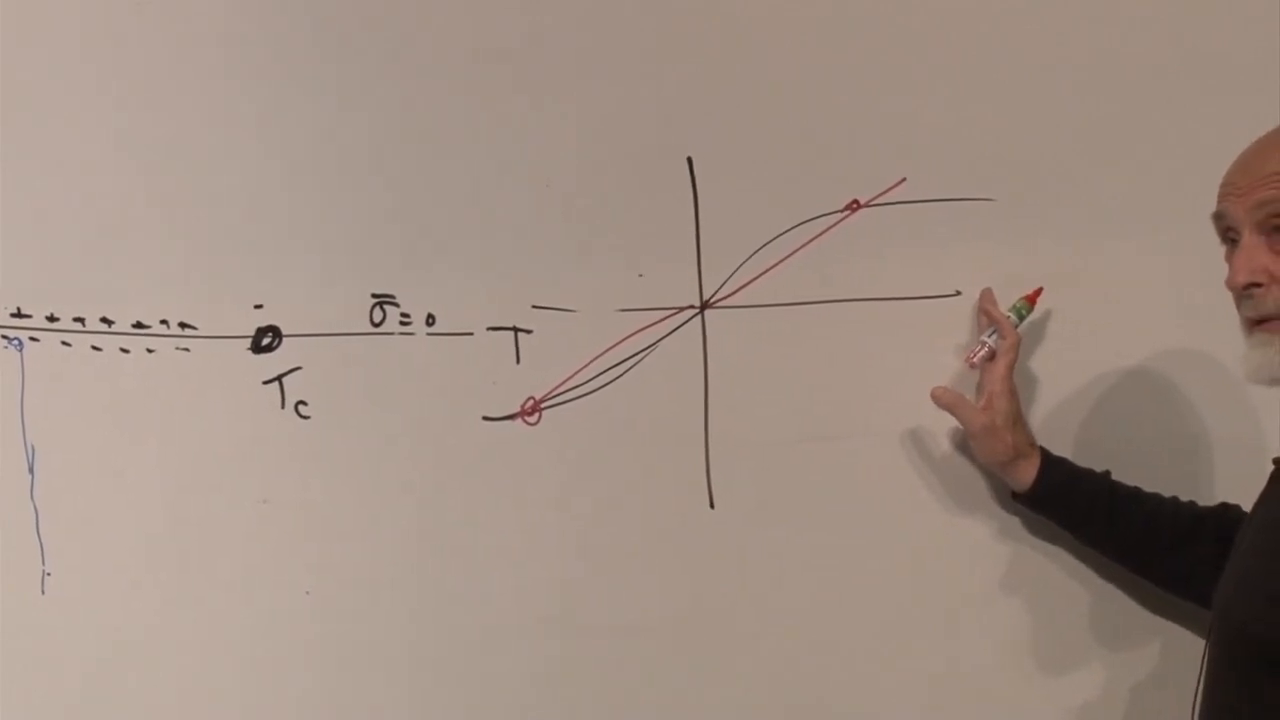
\includegraphics[width=0.90\textwidth]{lecture_10_figure_06.png}
\caption{\(T\)--\(h\) 平面中的共存线，以及温度低于 \(T_c\) 时固定温度下的磁化强度分支。}
\lectureframe{00:39:30}
\end{figure}

\begin{figure}[ht]
\centering
\resizebox{\linewidth}{!}{%
\begin{tikzpicture}[x=1.25cm,y=1.15cm]
\begin{scope}
\draw[->] (-2.45,0) -- (2.55,0) node[right] {$h$};
\draw[->] (0,0) -- (0,3.7) node[above] {$T$};
\draw[very thick,red!70!black] (0,0) -- (0,2.35);
\fill[red!70!black] (0,2.35) circle (2.3pt);
\node[right] at (0.08,2.35) {$T_c$};
\node at (-1.25,1.05) {$m>0$};
\node at (1.25,1.05) {$m<0$};
\draw[->,rounded corners,blue!65!black] (-1.65,0.85) -- (-1.65,3.02)
 -- (1.65,3.02) -- (1.65,0.85);
\node[blue!65!black] at (0,3.35) {continuous path};
\end{scope}
\begin{scope}[xshift=7.0cm,yshift=1.55cm]
\draw[->] (-2.5,0) -- (2.5,0) node[right] {$h$};
\draw[->] (0,-1.35) -- (0,1.4) node[above] {$m$};
\draw[very thick,blue!65!black]
  (-2.2,1.05) .. controls (-0.75,1.03) and (-0.2,0.75) .. (-0.08,0.62);
\draw[very thick,blue!65!black]
  (0.08,-0.62) .. controls (0.2,-0.75) and (0.75,-1.03) .. (2.2,-1.05);
\draw[dashed] (0,0.62) -- (0,-0.62);
\fill (0,0.62) circle (1.8pt);
\fill (0,-0.62) circle (1.8pt);
\node at (0,-1.75) {\(T<T_c\)};
\end{scope}
\end{tikzpicture}
}
\caption{在固定的 \(T<T_c\) 下，磁化强度在穿过共存线时发生跳变。而在完整的两参数平面中，两个相反而可以通过绕过临界点的方式连续地连接起来。}
\label{fig:ising-phase-plane}
\end{figure}

\begin{classroomqa}
\audiencequestion{如果在 \(T_c\) 以下磁场恰好为零，会发生什么？}
\lecturerresponse{理想的无限系统有两个同样好的纯相。任何与制备相关的无穷小残余偏置、边界条件或涨落都会选择其中之一。热力学不连续性由我们的符号约定中的两个单侧极限 \(m(T,0^-)=+m_0(T)\) 和 \(m(T,0^+)=-m_0(T)\) 来表示。\lecturetimestamp{00:35:04--00:37:10}}
\end{classroomqa}

\begin{classroomqa}
\audiencequestion{这和滞后是同一回事吗？}
\lecturerresponse{滞后涉及亚稳性以及真实系统切换分支时所表现出的依赖于历史的延迟。它与上述问题相关，但需要超出平衡相图的动力学，此处不予展开。\lecturetimestamp{00:37:11--00:37:20}}
\end{classroomqa}

\begin{classroomqa}
\audiencequestion{正相和负相能否在不穿过不连续点的情况下连接起来？}
\lecturerresponse{可以。将温度升高到 \(T_c\) 以上，在那里改变磁场的符号，然后再降低温度。这条路径绕过了端点，磁化强度连续地变化。只有当在固定的 \(T<T_c\) 下穿过 \(h=0\) 时，跳变才是不可避免的。\lecturetimestamp{00:37:20--00:38:15}}
\end{classroomqa}

\begin{classroomqa}
\audiencequestion{每当 \(h\) 趋近于零时，磁化强度都会趋近于零吗？}
\lecturerresponse{在 \(T_c\) 以下的一般温度下并非如此。在那里，单侧极限不为零。自发磁化强度只有在临界温度本身被趋近时才会趋近于零。\lecturetimestamp{00:38:29--00:39:45}}
\end{classroomqa}

\section{可渗透盒子与化学势}

现在我们离开磁体，重新从粒子开始。设想一个区域，其势能低于周围空间的势能。壁是可渗透的：粒子可以进入和离开。如果内部能量低了 \(\mu\)，那么内部占据会获得一个相对的玻尔兹曼因子 \(e^{\beta\mu}\)。加深或抬高势阱会改变盒子中粒子的平均数目。

\begin{figure}[ht]
\centering
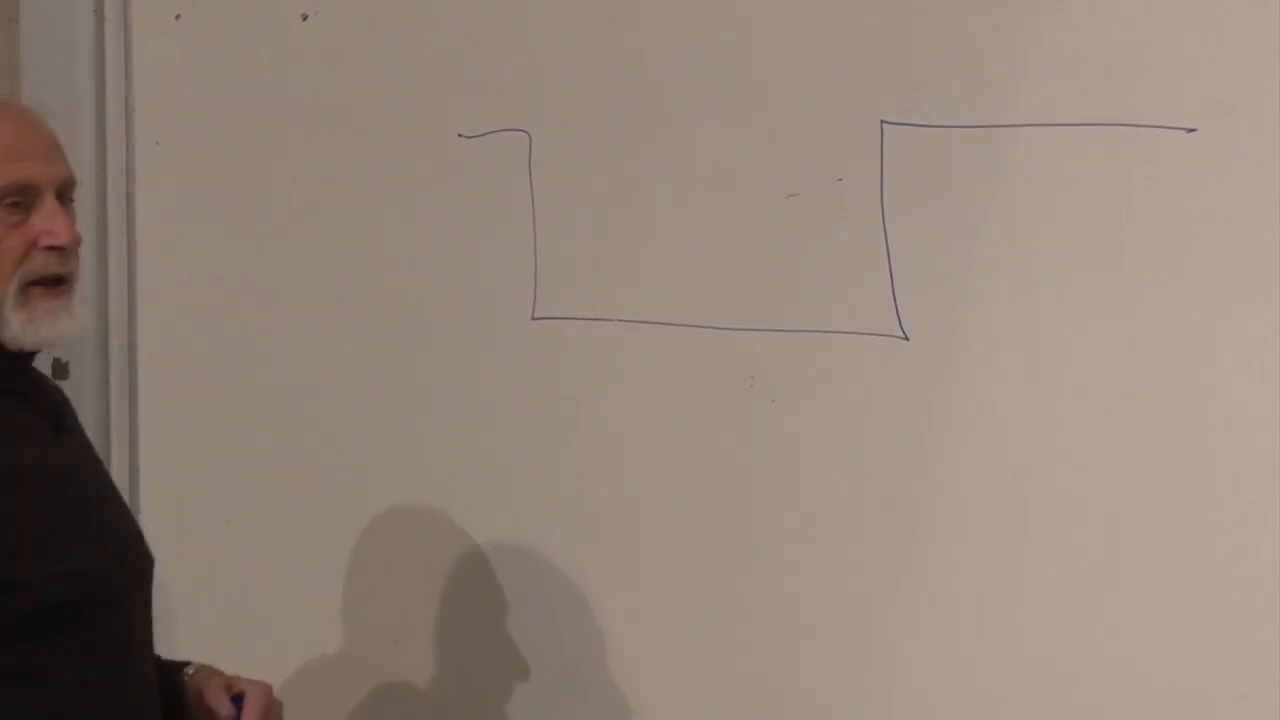
\includegraphics[width=0.84\textwidth]{lecture_10_figure_07.png}
\caption{可渗透盒子的势阱图像。内部与外部之间的能量差控制着粒子占据盒子的倾向。}
\lectureframe{00:41:30}
\end{figure}

\begin{figure}[ht]
\centering
\resizebox{\linewidth}{!}{%
\begin{tikzpicture}[x=1.25cm,y=1.0cm]
\draw[->] (-3.2,0) -- (3.3,0) node[right] {position};
\draw[->] (-3.0,-2.4) -- (-3.0,1.2) node[above] {potential};
\draw[very thick] (-2.8,0.7) -- (-1.35,0.7)
 -- (-1.35,-1.45) -- (1.35,-1.45) -- (1.35,0.7) -- (2.9,0.7);
\draw[<->,red!70!black] (0,0.63) -- (0,-1.38);
\node[right,red!70!black] at (0.08,-0.35) {$\mu$};
\foreach \x/\y in {-0.95/-1.1,-0.45/-0.85,0.05/-1.12,0.55/-0.95,0.95/-1.18}
  \fill[blue!65!black] (\x,\y) circle (2pt);
\node at (0,-2.0) {permeable region};
\end{tikzpicture}
}
\caption{改变势偏移会改变粒子数偏好。在巨正则描述中，该偏移由化学势表示。}
\end{figure}

这个思想实验使化学势变得具体。它是相对于粒子库而言，每增加一个粒子所获得的能量优势。如果多种粒子种类能够穿过壁，那么每种粒子种类都有自己的化学势。密封盒子则不同：此时 \(N\) 是固定的，化学势是通过热力学推断出来的，而不是通过与粒子库的交换来施加的。

\begin{classroomqa}
\audiencequestion{势阱的深度就是化学势吗？}
\lecturerresponse{它是化学势差的一种直接力学实现。将内部每一个单粒子能级降低 \(\mu\)，会对能量贡献 \(-\mu N\)，因此对玻尔兹曼指数贡献 \(+\beta\mu N\)。只有化学势的差值才有意义。\lecturetimestamp{00:44:49--00:45:40}}
\end{classroomqa}

由于粒子可以进入和离开，配分和必须包含所有粒子数：
\begin{equation}
\Xi(T,\mu)
=\sum_{N=0}^{\infty}\;\sum_{\mathcal C_N}
\exp\!\left[-\beta E(\mathcal C_N)+\beta\mu N\right].
\label{eq:grand-partition}
\end{equation}
内层求和遍历具有指定 \(N\) 的构型；外层求和遍历 \(N\) 本身。巨正则权重也可以写成 \(e^{-\beta(E-\mu N)}\)。

\begin{figure}[ht]
\centering
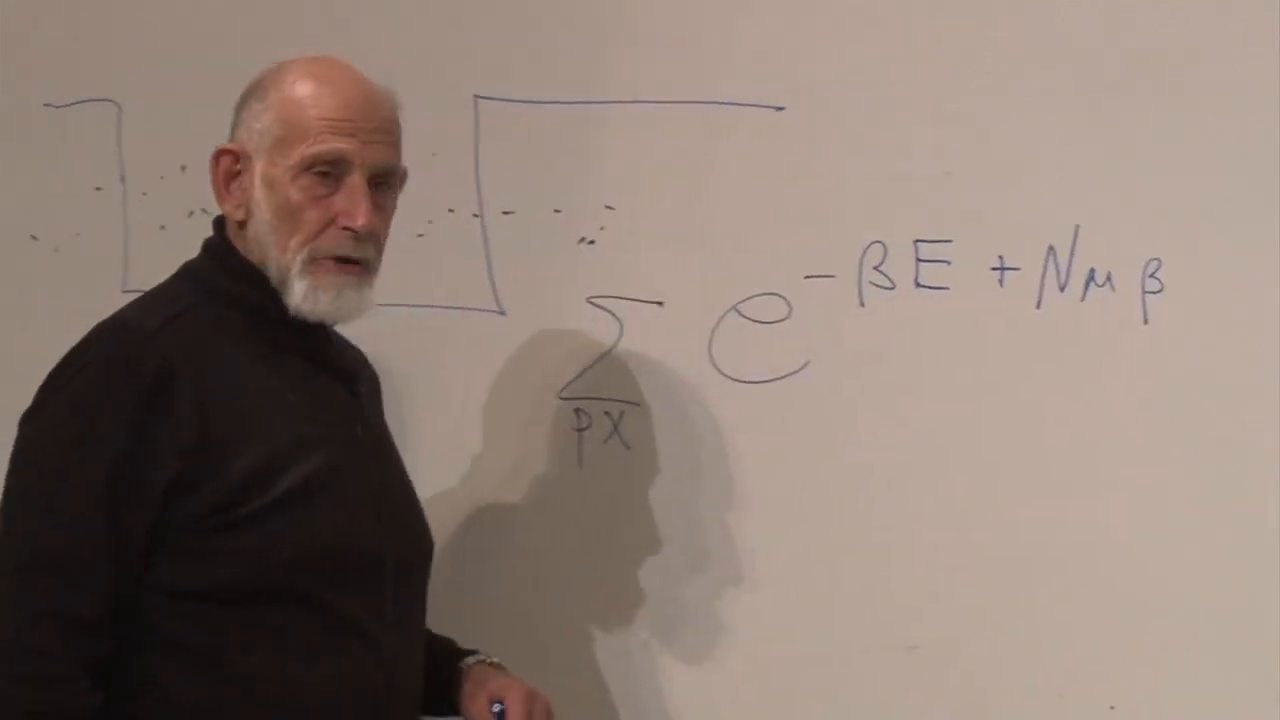
\includegraphics[width=0.88\textwidth]{lecture_10_figure_08.png}
\caption{可渗透盒子以及对粒子数和构型的巨正则求和。}
\lectureframe{00:47:15}
\end{figure}

\begin{classroomqa}
\audiencequestion{当盒子被密封时，会有什么变化？}
\lecturerresponse{粒子数不再涨落。此时使用固定 \(N\) 下的正则配分函数。在可渗透盒子中，\(N\) 是一个热力学变量，其平均值由 \(\mu\) 控制。\lecturetimestamp{00:45:42--00:47:50}}
\end{classroomqa}

在固定温度下，改变 \(\mu\) 通常会使密度平滑变化。低于临界温度时，它反而可能引起突变。这正是我们要寻找的流体现象。为了从微观上得到它，粒子需要两个特征：它们不能占据同一位置，并且必须在短程上相互吸引。

\section{将自旋转化为点阵气体}

保留点阵，但重新解释它的两个状态。定义占据数
\begin{equation}
n_i=\frac{1+\sigma_i}{2}
=
\begin{cases}
0,&\sigma_i=-1,\\
1,&\sigma_i=+1.
\end{cases}
\label{eq:occupation-map}
\end{equation}
空位点具有自旋向下；被占据的位点具有自旋向上。由于 \(n_i\) 只能为零或一，双重占据被禁止。因此点阵本身提供了硬核。

\begin{figure}[ht]
\centering
\includegraphics[width=0.84\textwidth]{lecture_10_figure_04.png}
\caption{点阵气体的对应从 \(\sigma=-1\) 表示空位点开始；\(\sigma=+1\) 则表示被占据的位点。}
\lectureframe{00:53:45}
\end{figure}

从空点阵开始，所有 \(\sigma=-1\)。每条键都对齐，能量为 \(-J\)。这个恒定的真空能量可以被减去。现在在二维中把一个粒子放在一个位点上。相应的自旋翻转到 \(+1\)，破坏了四条键。每条被破坏的键代价为 \(2J\)，所以
\begin{equation}
\Delta E_1=4(2J)=8J.
\label{eq:one-particle-cost}
\end{equation}
两个相距很远的粒子破坏八条键，代价为 \(16J\)。如果这两个粒子占据相邻位点，它们之间的键重新对齐。只有六条边界键被破坏，代价为
\begin{equation}
\Delta E_{2,\rm adjacent}=6(2J)=12J.
\end{equation}
因此，把粒子拉到一起会使能量降低
\begin{equation}
16J-12J=4J.
\label{eq:lattice-attraction}
\end{equation}
这个实时计数最初被描述为 \(2J\) 的节省，随后得到更正：一条共享的键消除了两个被破坏边界的贡献，因此吸引为 \(4J\)。

\begin{figure}[ht]
\centering
\includegraphics[width=0.84\textwidth]{lecture_10_figure_05.png}
\caption{二维键计数：一个孤立粒子代价为 \(8J\)，两个远离的粒子代价为 \(16J\)，两个相邻粒子代价为 \(12J\)。}
\lectureframe{01:00:25}
\end{figure}

点阵气体现在具有两个所需的分子性质。二元占据提供了硬核排斥，交换相互作用提供了强度为 \(4J\) 的最近邻吸引。粒子数被允许涨落，因为自旋翻转会改变被占据位点的数目。

\subsection{精确的代数对应词典}

键计数图像足以看出物理，但精确的变量替换使等价性无可置疑。将
\begin{equation}
\sigma_i=2n_i-1
\end{equation}
代入方程 ~\eqref{eq:ising-hamiltonian}。对于一条键，
\begin{equation}
\sigma_i\sigma_j
=4n_in_j-2n_i-2n_j+1.
\end{equation}
在规则的 \(d\) 维点阵上，
\begin{equation}
\sum_{\langle ij\rangle}(n_i+n_j)=2d\sum_i n_i.
\end{equation}
因此
\begin{align}
\mathcal H
&=-4J\sum_{\langle ij\rangle}n_in_j
+(4dJ+2h)\sum_i n_i+\text{constant}.
\label{eq:ising-as-lattice-gas}
\end{align}
将其与常规的点阵气体哈密顿量
\begin{equation}
\mathcal H_{\rm lg}
=-\epsilon\sum_{\langle ij\rangle}n_in_j
-\mu\sum_i n_i+\text{constant}.
\label{eq:lattice-gas-hamiltonian}
\end{equation}
比较。对应词典为
\begin{equation}
\boxed{\epsilon=4J,\qquad
\mu=-(4dJ+2h).}
\label{eq:chemical-potential-map}
\end{equation}

\begin{figure}[ht]
\centering
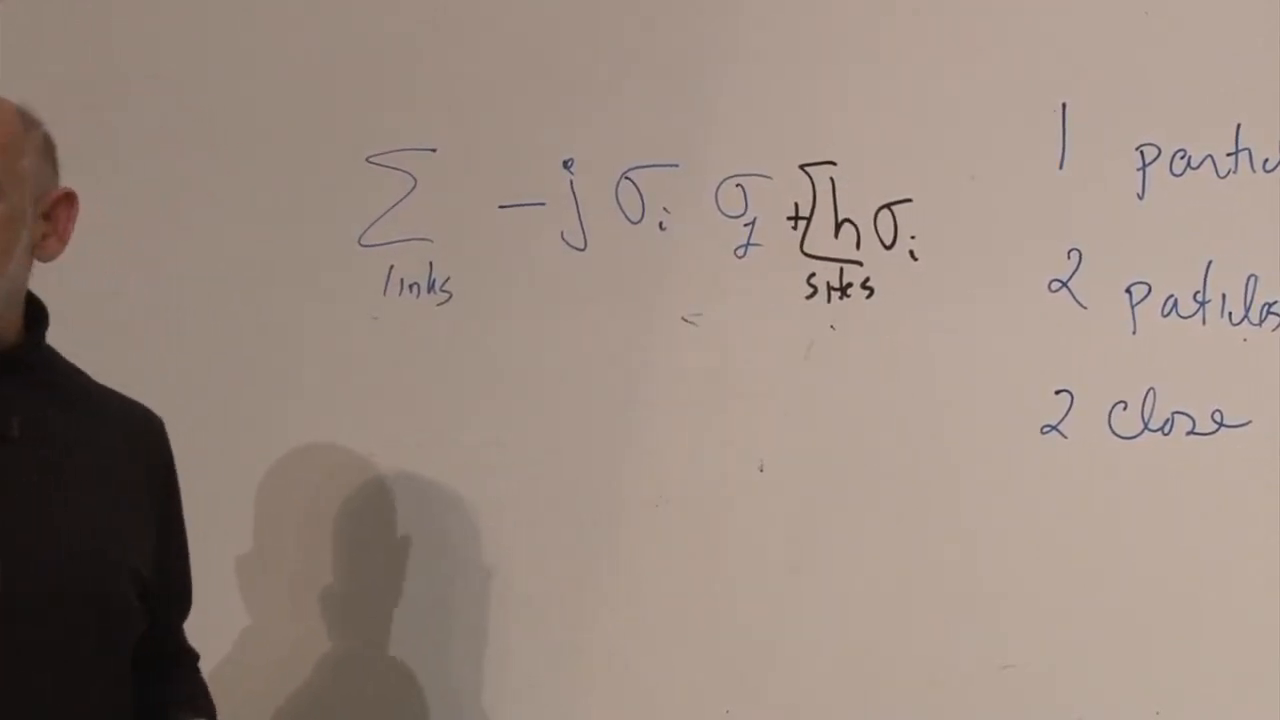
\includegraphics[width=0.88\textwidth]{lecture_10_figure_09.png}
\caption{交换项和场项与粒子能量计数并列。场改变插入能量，而不改变最近邻吸引。}
\lectureframe{01:04:30}
\end{figure}

在二维中，一次孤立插入使能量改变
\begin{equation}
8J+2h=-\mu.
\end{equation}
\(8J\) 来自被破坏的键；\(2h\) 来自将一个自旋从 \(-1\) 变为 \(+1\)。因此，调节 \(h\) 会调节化学势，同时保持吸引 \(4J\) 固定。场并不字面等于 \(\mu\)，因为交换基线贡献了偏移 \(4dJ\)。

\begin{classroomqa}
\audiencequestion{如果场控制粒子数，为什么 \(h\) 不简单地就是化学势？}
\lecturerresponse{创建一个粒子相对于空参考态也会破坏交换键。因此 \(-N\) 的常规系数是 \(\mu=-(4dJ+2h)\)，而不仅仅是 \(-2h\)。该偏移取决于 \(J\) 和配位数。\lecturetimestamp{01:06:28--01:06:41}}
\end{classroomqa}

密度同样简单：
\begin{equation}
\rho=\expect{n_i}
=\frac{1+\expect{\sigma_i}}{2}
=\frac{1+m}{2}.
\label{eq:density-map}
\end{equation}
因此 \(m=-1\) 是空点阵，\(m=+1\) 是完全填满的点阵，而 \(m=0\) 是半填充。总粒子数为 \(N_{\rm p}=\sum_i n_i\)；密度为 \(N_{\rm p}/N\)。

\begin{figure}[ht]
\centering
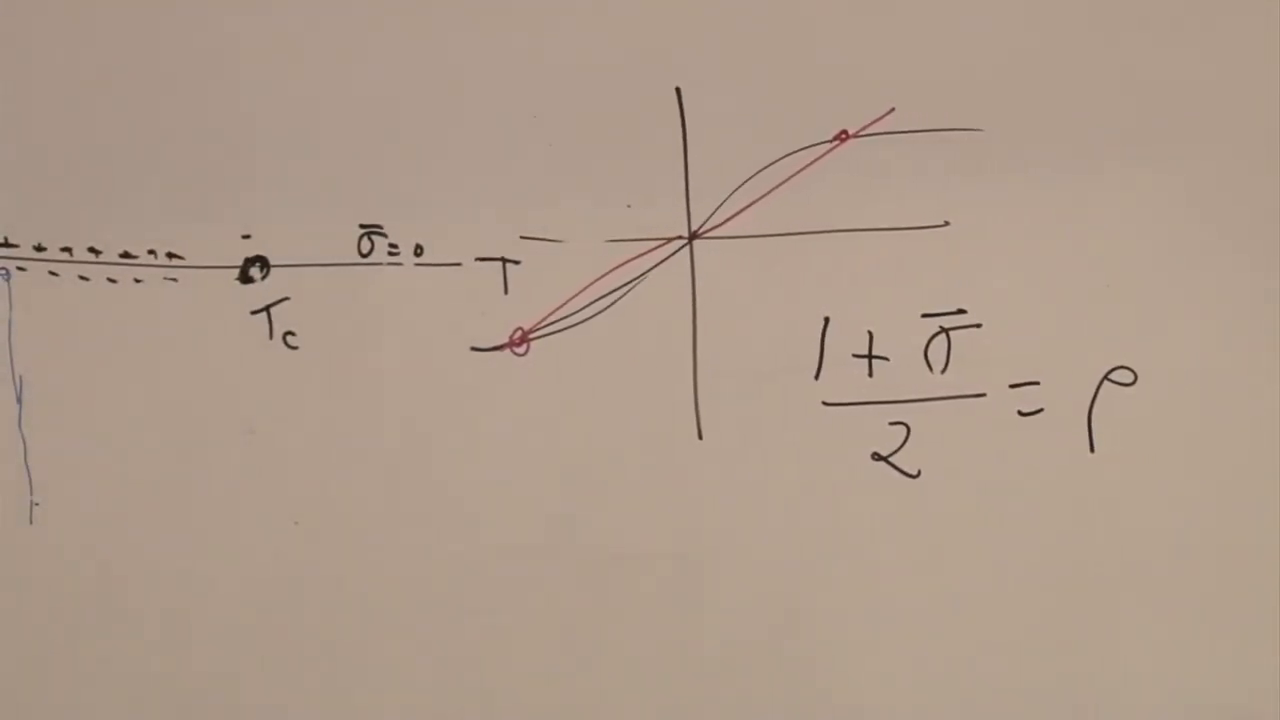
\includegraphics[width=0.90\textwidth]{lecture_10_figure_10.png}
\caption{密度关系 \(\rho=(1+m)/2\) 写在磁共存线旁边。}
\lectureframe{01:08:25}
\end{figure}

\begin{classroomqa}
\audiencequestion{\((1+m)/2\) 是粒子数还是密度？}
\lecturerresponse{它是每个位点的平均占据数，因此是无量纲的点阵密度。乘以总位点数就得到预期的粒子数。区分强度量密度和广延量计数很重要。\lecturetimestamp{01:06:43--01:09:31}}
\end{classroomqa}

\section{磁相图变为流体相图}

利用方程 ~\eqref{eq:chemical-potential-map} 和 \eqref{eq:density-map} 翻译图 ~\ref{fig:ising-phase-plane}。在 \(T_c\) 以上，改变 \(\mu\) 会平滑地改变密度。在 \(T_c\) 以下，越过共存值
\begin{equation}
\mu_{\rm coex}=-4dJ
\qquad(h=0)
\label{eq:coexistence-mu}
\end{equation}
会使密度在稀薄气体和稠密液体之间跳跃。在 \(T_c\) 处，两个密度合并，不连续性消失。

\begin{figure}[ht]
\centering
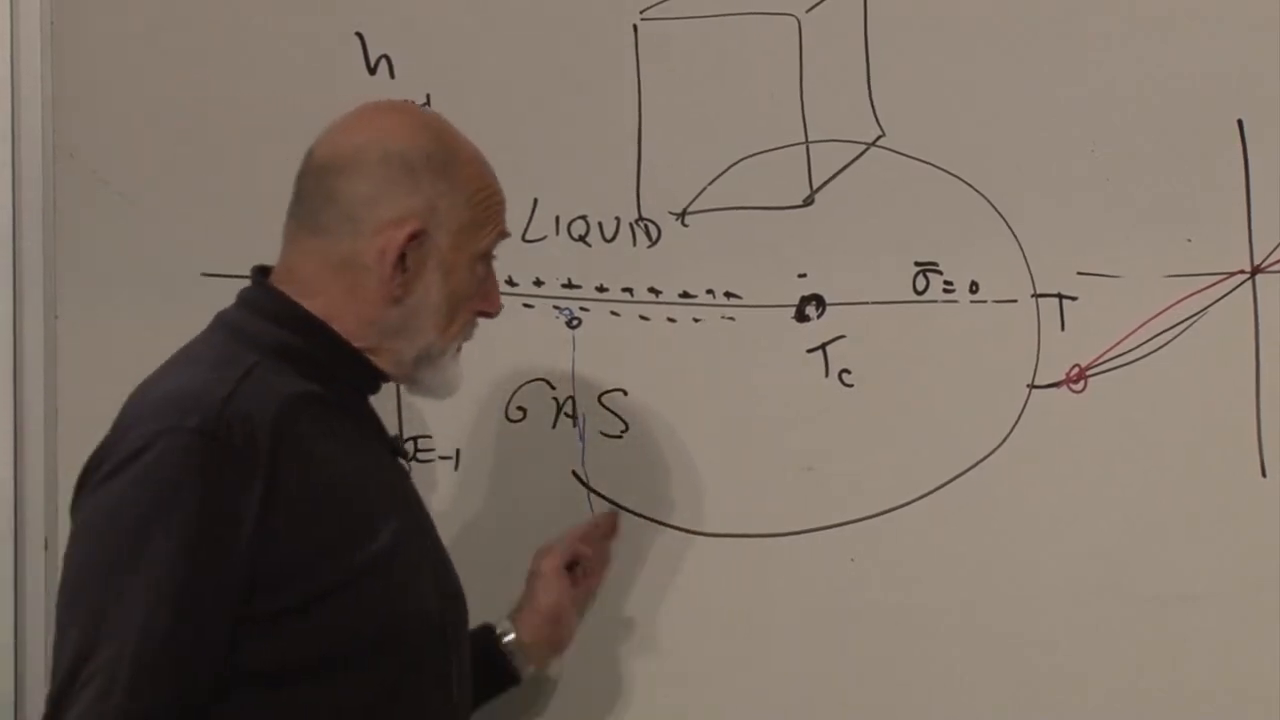
\includegraphics[width=0.92\textwidth]{lecture_10_figure_11.png}
\caption{伊辛共存线被解读为液--气相图。气体位于低密度一侧，液体位于高密度一侧，二者可以绕过临界端点连续地连接起来。}
\lectureframe{01:14:30}
\end{figure}

\begin{figure}[ht]
\centering
\begin{tikzpicture}[x=1.25cm,y=1.1cm]
\draw[->] (-2.65,0) -- (2.75,0) node[right] {$\mu-\mu_{\rm coex}$};
\draw[->] (0,0) -- (0,3.8) node[above] {$T$};
\draw[very thick,red!70!black] (0,0) -- (0,2.35);
\fill[red!70!black] (0,2.35) circle (2.4pt);
\node[right] at (0.1,2.35) {critical point};
\node at (-1.35,1.0) {gas};
\node at (1.35,1.0) {liquid};
\draw[->,blue!65!black,rounded corners]
 (-1.7,0.85) -- (-1.7,3.05) -- (1.7,3.05) -- (1.7,0.85);
\node[blue!65!black] at (0,3.4) {continuous route};
\end{tikzpicture}
\caption{在端点以下，液体和气体是彼此不同的相，但在超临界区域，并没有奇异的边界将它们分开。}
\label{fig:liquid-gas-plane}
\end{figure}

这就识别出了我们所熟悉的沸腾线。在固定压强下，将液体加热至越过共存线便产生沸腾。在固定温度下，改变压强或化学势也可以越过同一条边界。过热蒸气或过冷液体是超出平衡共存线的亚稳态延续；描述其寿命需要成核动力学，这超出了本平衡态构造的范围。

\begin{classroomqa}
\audiencequestion{过热蒸汽在这个相图中有所体现吗？}
\lecturerresponse{平衡相图标示的是共存边界。过热或过饱和状态是亚稳态的：它暂时停留在错误的一侧，因为形成临界液滴需要付出界面自由能的代价。这种动力学上的修正此处不予计算。 \lecturetimestamp{01:12:19--01:12:29}}
\end{classroomqa}

\begin{classroomqa}
\audiencequestion{在普通流体中，人们如何改变化学势？}
\lecturerresponse{势阱盒子是干净的理论控制手段。在实验室中，人们更常改变压强、体积或与热库的接触；热力学随后会将这些控制量转化为化学势的变化。 \lecturetimestamp{01:12:30--01:13:59}}
\end{classroomqa}

\begin{classroomqa}
\audiencequestion{当密度改变时，我们是在改变分子势 \(J\) 吗？}
\lecturerresponse{不是。对于固定的一种物质，\(J\) 代表短程吸引，并且在这个模型中保持不变。改变 \(\mu\) 会改变有多少格点被占据，从而改变分子间间距的分布。改变 \(J\) 则意味着改变微观物质或相互作用。 \lecturetimestamp{01:14:50--01:15:41}}
\end{classroomqa}

\begin{classroomqa}
\audiencequestion{临界温度和通常所说的沸点是同一回事吗？}
\lecturerresponse{不是。沸点是在选定的压强下确定的，因此当压强改变时，它沿共存曲线移动。临界温度是唯一的端点，高于它液体和气体不再被相边界分开。在这个点阵气体处理中，压强尚未被显式地推导出来。 \lecturetimestamp{01:15:42--01:17:02}}
\end{classroomqa}

现在可以陈述核心结果了。伊辛磁体与点阵气体并不只是画出相似的相图。在变量和参数变换之后，它们共享同一个配分函数。一侧的每一个奇异热力学性质在另一侧都有对应物：
\begin{equation}
\begin{array}{c|c}
\text{Ising magnet} & \text{lattice gas}\\ \hline
\sigma_i=\pm1 & n_i=0,1\\
m=\expect{\sigma} & \rho=(1+m)/2\\
h & \mu=-(4dJ+2h)\\
\text{aligned exchange} & \text{nearest-neighbor attraction}\\
h=0,\ T<T_c & \text{liquid--gas coexistence}\\
(T_c,0) & \text{critical endpoint}
\end{array}
\label{eq:ising-fluid-dictionary}
\end{equation}

\section{临界指数与普适性}

在临界点附近，热力学量常常出现幂律奇异性。以约化温度
\begin{equation}
t=\frac{T-T_c}{T_c},
\end{equation}
可示意性地写出
\begin{equation}
m\sim(-t)^{\beta_{\rm crit}},
\qquad
\chi\sim |t|^{-\gamma},
\qquad
\xi\sim |t|^{-\nu}.
\label{eq:critical-exponents}
\end{equation}
这里 \(\beta_{\rm crit}\) 是临界指数，而不是温度的倒数。平均场给出 \(\beta_{\rm crit}=1/2\)，但在上临界维度以下，涨落会改变这些指数。

这些指数不必是整数。它们也不必都是无理数：二维伊辛模型以拥有若干精确的有理指数而闻名，而三维伊辛模型的指数则是通过理论和计算以高精度确定下来的非平凡数值。稳健的教训是，这些指数一般并不由初等的量纲分析所固定。

更引人注目的是，微观细节往往也不能固定它们。具有相同空间维度、相同序参量对称性以及足够短程相互作用的系统，可以流向同一个长距离临界理论。它们属于同一个 \emph{普适类}。单轴磁体和普通液--气端点都具有单个标量序参量，并在相同维度下共享伊辛普适类。

\begin{classroomqa}
\audiencequestion{普适类是有限的还是离散的清单？}
\lecturerresponse{普适类有很多，按维度、对称性、守恒律、相互作用程以及其他长距离数据来组织。在许多熟悉的情形中，不动点和指数集合是离散的，但也存在指数连续变化的系统。稳妥的说法并不是这个目录是有限的；而是许多微观上不同的系统共享相同的长距离数据。 \lecturetimestamp{01:18:50--01:19:38}}
\end{classroomqa}

\begin{classroomqa}
\audiencequestion{如果液体和气体共存，在实际容器中是什么把它们分开？}
\lecturerresponse{是界面。表面张力对界面面积施加惩罚，而重力产生竖直的化学势梯度，通常使较密的液体位于气体下方。在重力可忽略时，几何形状更直接地由表面张力和边界条件控制。\lecturetimestamp{01:19:40--01:21:18}}
\end{classroomqa}

\begin{classroomqa}
\audiencequestion{在这幅图像中，汽化热在哪里？}
\lecturerresponse{在临界点以下，穿过一阶共存线通常会伴随潜热。当接近临界端点时，汽化热趋于零，因为两相在那里变得相同。本讲建立了相结构，但没有计算潜热。\lecturetimestamp{01:21:19--01:22:18}}
\end{classroomqa}

\begin{classroomqa}
\audiencequestion{相变能否用作灵敏探测器，例如用超导器件？}
\lecturerresponse{可以。在相变附近，微小的扰动可以产生很大的响应，或触发状态改变。实用探测器正是利用这种灵敏度，尽管相关的序参量和动力学可能与伊辛例子不同。\lecturetimestamp{01:22:19--01:24:05}}
\end{classroomqa}

统计力学课程到此结束。这条路线从熵和平衡开始，经过配分函数和气体，最后表明磁体和流体可以是同一临界现象的两种描述。

\section{课后讨论：精细调节与选择}

正式讲座结束后，谈话又持续了大约四十分钟。它值得保留，但不应与上面的推导相混淆。主题不再是点阵气体，而是精细调节的逻辑以及宇宙学中人类选择原理的谨慎使用。

\subsection{小数字并不自动意味着精细调节}

没有任何一句话能解决\emph{人类原理}这一短语的每一种用法。有用的起点是操作性的：当一个理论允许许多被实现的环境时，观测要以观察者只能在其中一些环境中出现这一事实为条件。这种条件陈述可以是理性的。如果没有任何系综、选择条件或使替代方案具有物理意义的机制就援引它，它就会变得空洞。

在选择介入之前，必须区分小参数和精细调节参数。一个数可以因为稳定的动力学机制把它驱动到某个特殊值而很小。精细调节意味着，观测值似乎要求在其他方面相互独立的贡献之间达到极其精确的平衡，而没有任何已知的恢复机制或对称性保护这种平衡。

\begin{classroomqa}
\audiencequestion{人类原理能否被精确地表述？}
\lecturerresponse{它站得住脚的用法是条件性的，而不是神秘的：如果许多物理上被实现的环境具有不同的参数，那么像我们这样的存在者所观测到的环境就是从与观察者相容的子集中抽取出来的。这本身并不产生这些环境，也不赋予它们概率；那些任务属于底层物理学。\lecturetimestamp{01:25:45--01:26:13}}
\end{classroomqa}

宇宙学常数是引发这一讨论的例子。与朴素的量子场论对真空能的贡献相比，它的观测值极其微小。困难不仅在于最终的数字很小，而在于许多大项似乎必须以极高的精度相消，同时没有任何公认的低能反馈机制把结果调整到观测值。

\subsection{飞艇与潜艇}

两个浮力例子把这一区分孤立出来。飞艇漂浮在其平均密度与周围空气密度相匹配的高度。空气密度随高度降低。如果飞艇上升，外部空气变得较稀薄，飞艇趋于下降；如果它下降，外部空气变得较稠密，飞艇趋于上升。密度匹配在数值上可能很微妙，但大气梯度提供了恢复反馈。该平衡得到了动力学解释。

在几乎不可压缩的水中处于中性浮力的潜艇则不同。水的密度随深度变化很小。如果潜艇的平均密度恰好等于周围水的密度，并没有可比的、依赖深度的恢复机制来解释这种相等。微小的失配就会使它上升或下沉。实现中性浮力需要精确调整压载物和装载物。于是，除非某种控制系统或设计机制对此作出解释，否则这个微小的残差就是精细调节。

\begin{figure}[ht]
\centering
\resizebox{\linewidth}{!}{%
\begin{tikzpicture}[>=Latex]
\begin{scope}[xshift=-3.8cm]
\shade[top color=blue!5,bottom color=blue!28] (-2.5,-2.2) rectangle (2.5,2.2);
\draw[very thick,rounded corners=18pt,fill=yellow!35]
  (-1.15,0) ellipse (1.15 and 0.55);
\draw[thick] (0,-0.55) -- (0,-1.05);
\draw[thick,fill=gray!20] (-0.45,-1.05) rectangle (0.45,-1.38);
\draw[->,red!70!black,thick] (1.65,1.45) -- (1.65,0.55)
 node[midway,right] {restoring};
\draw[->,red!70!black,thick] (-1.65,-1.45) -- (-1.65,-0.55)
 node[midway,left] {restoring};
\node at (0,2.55) {\textbf{Blimp: density gradient}};
\node[align=center] at (0,-2.75) {displacement changes\\the buoyant imbalance};
\end{scope}
\begin{scope}[xshift=3.8cm]
\shade[top color=cyan!10,bottom color=blue!45] (-2.5,-2.2) rectangle (2.5,2.2);
\draw[very thick,fill=gray!35,rounded corners=12pt]
  (-1.45,-0.25) -- (1.1,-0.25) arc (-90:90:0.38)
  -- (-1.45,0.51) -- cycle;
\draw[thick] (-0.25,0.51) -- (-0.25,0.85) -- (0.35,0.85) -- (0.35,0.51);
\draw[->,red!70!black,thick] (1.65,0.15) -- (1.65,1.35)
 node[midway,right] {rise};
\draw[->,red!70!black,thick] (-1.65,0.15) -- (-1.65,-1.35)
 node[midway,left] {sink};
\node at (0,2.55) {\textbf{Submarine: nearly uniform density}};
\node[align=center] at (0,-2.75) {no depth-dependent feedback\\protects neutral buoyancy};
\end{scope}
\end{tikzpicture}
}
\caption{微小的残余量既可以是动力学上稳定的，也可以是真正经过精细调节的。飞艇具有恢复性反馈；理想化潜艇则要求其平均密度被调节到与水的密度相匹配。}
\label{fig:blimp-submarine}
\end{figure}

\begin{classroomqa}
\audiencequestion{如果观察到中性浮力，潜艇乘员为什么应当要求一个解释？}
\lecturerresponse{因为，在缺乏压载控制机制的情况下，既没有对称性也没有环境反馈来保护两个独立密度的相等性。问题不在于这种相等在逻辑上是否可能，而在于系统为什么占据其参数空间中如此狭窄的一个区域。\lecturetimestamp{01:35:05--01:36:25}}
\end{classroomqa}

\subsection{众多域与条件性观测}

现在设想一个过程，它产生数量极其庞大的潜艇，且这些潜艇具有许多不同的平均密度。大多数会下沉或上浮；只有极小一部分能在水面与海底之间适宜生存的带中长期停留。一个必然生活在幸存潜艇之一的观测者，在测得接近中性浮力时不应感到惊讶。这一观测被观测者得以存在所要求的条件所选择。

这一推理需要两个要素：
\begin{enumerate}
\item 一个实际实现许多备选可能性的物理过程，而不是仅存在于想象中的备选可能性；
\item 一个选择条件，用以解释为什么观测只在某个受限子集中进行。
\end{enumerate}
选择并不取代产生机制。一旦系综存在，它改变的是观测者测得某物的条件概率。

\begin{classroomqa}
\audiencequestion{这个论证仅仅是在说，在足够大的样本中，某处会发生不太可能的事情吗？}
\lecturerresponse{这只是前半部分。后半部分是观测条件化：观测者并非从所有域中均匀抽样，而只是从他们的存在成为可能的那些域中抽样。一个完整的方案仍然需要域上的测度，以及关于它们如何被产生的物理解释。\lecturetimestamp{01:39:19--01:40:36}}
\end{classroomqa}

应用于真空能时，一个大的负宇宙学常数可以使宇宙过快再坍缩，而一个足够大的正值则可以阻止物质凝聚成星系。观测值位于与长寿命结构相容的狭窄范围内。这提供了一个可能的选择条件，而不是对宇宙学常数分布的推导。

量子场论增加了精细调节问题：来自不同场和尺度的真空贡献各自都远大于观测到的残余量。如果这些项几乎完全相消，结果就更像精心平衡的潜艇，而不是自我校正的飞艇。这一类比意在揭示逻辑问题，而不是提供其解决方案。

\begin{classroomqa}
\audiencequestion{一个参数的变化能否由其他几个参数的变化来补偿？}
\lecturerresponse{能。可存活集不必是一个轴上的狭窄区间；它可以是多维参数空间中的一张薄曲面。相关变化可以保持结构，但问题于是变成：为什么实际实现的参数位于该曲面附近，以及底层理论赋予它的测度是什么。\lecturetimestamp{01:45:10--01:46:19}}
\end{classroomqa}

\begin{figure}[ht]
\centering
\begin{tikzpicture}[x=1.3cm,y=1.05cm,>=Latex]
\draw[->] (-3.2,0) -- (3.4,0) node[right] {$\lambda_1$};
\draw[->] (0,-2.5) -- (0,2.65) node[above] {$\lambda_2$};
\fill[gray!12] (-3,-2.25) rectangle (3.1,2.3);
\draw[very thick,blue!65!black]
 (-2.8,-1.55) .. controls (-1.3,-0.75) and (0.15,0.05) .. (2.85,1.55);
\draw[very thick,blue!25]
 (-2.8,-1.25) .. controls (-1.3,-0.45) and (0.15,0.35) .. (2.85,1.85);
\fill[blue!15,opacity=.65]
 (-2.8,-1.55) .. controls (-1.3,-0.75) and (0.15,0.05) .. (2.85,1.55)
 -- (2.85,1.85) .. controls (0.15,0.35) and (-1.3,-0.45) .. (-2.8,-1.25) -- cycle;
\node[blue!65!black,rotate=28] at (1.3,0.95) {viable band};
\foreach \x/\y in {-2.4/1.45,-1.7/-1.8,-0.9/1.8,0.3/-1.45,1.2/1.85,2.4/-0.8}
  \fill[red!65!black] (\x,\y) circle (2pt);
\fill[green!45!black] (0.55,0.58) circle (2.8pt);
\node[green!35!black,right] at (0.65,0.55) {observed domain};
\end{tikzpicture}
\caption{在存在多个参数时，可居住性或结构可存活性可能占据一条薄的相关带，而不是某一个参数的狭窄区间。选择将观测限制在该带内，但并不产生参数分布。}
\label{fig:viable-parameter-band}
\end{figure}

\subsection{景观式提议及其不确定性}

备选可能性的一种被提议来源是具有许多亚稳真空的理论，这些真空可能在不同宇宙域中被占据。弦论景观思想和永恒暴胀情景是例子，但它们的详细实现和概率测度仍然不确定。本讲将其作为一种可能性提出，而不是既定事实。

如果对称性迫使宇宙学常数精确为零，那将是一种更常规的解释。困难在于，观测到的加速膨胀对应一个小的非零值。一个自然地给出精确零的机制并不会自动解释微小的残余量；破缺该对称性可能只是重新引入精细调节。潜艇的意象在这里重新出现：一根绳索可以把它保持在选定的深度，但那样一来，绳索就是必须被识别出来而不是被假定的机制。

\begin{classroomqa}
\audiencequestion{非常精确地测量一个参数会违反不确定性原理吗？}
\lecturerresponse{不会。不确定性关系适用于特定的非对易可观测量对。一个耦合常数或真空参数可以具有被精确确定的值，而不必是某个不受控制的可观测量的正则共轭量。精确性本身并不是不确定性原理的悖论。\lecturetimestamp{01:49:21--01:49:36}}
\end{classroomqa}

\begin{classroomqa}
\audiencequestion{人择推理是解释了该值，还是仅仅重述了观测者需要它？}
\lecturerresponse{仅凭选择并不是一种动力学解释。它的正当作用是在一个物理上实现了的系综中改变条件概率。若在没有系综、没有测度、也没有可检验后果的情况下使用，它就有沦为标签而非解释的风险。\lecturetimestamp{01:49:37--01:50:21}}
\end{classroomqa}

\subsection{粒子物理中的中等程度巧合}

并非每一个与生命相关的参数都被调到同样非凡的程度。普通物质依赖于光子、电子、轻夸克和强相互作用；中微子影响宇宙学，但并不是原子的直接束缚媒介。质子--中子质量差尤其具有重大后果。因为中子比质子略重，孤立中子可以衰变，而普通氢是稳定的。若把这一顺序反转足够多，就会从根本上改变核化学。

电子质量和精细结构常数同样决定了原子尺度和结合能。大幅改变它们会改变化学。这些都是有意义的敏感性陈述，但不应当被夸大为这样一种主张：每一个微小的变化都会禁止一切可以设想的复杂性形式。与宇宙学常数问题相比，许多这类巧合都是中等程度的，并且与其他参数相关联。

与电弱尺度相关的等级问题是另一个突出的自然性问题：辐射贡献倾向于使一个基本标量质量对高尺度敏感，除非受到额外结构的保护。它的地位和解释不同于真空能问题，二者都不应被化约为一句口号。

\begin{classroomqa}
\audiencequestion{改变质子--中子质量差真的会对普通物质有影响吗？}
\lecturerresponse{会。观测到的顺序允许稳定的氢存在，并控制着原子核中的贝塔稳定性。适度的改变可以重新组织核丰度和恒星燃烧。仔细的分析必须一致地改变相互耦合的参数，而不是改变一个数值而把其余一切都冻结不变。\lecturetimestamp{01:51:47--01:53:08}}
\end{classroomqa}

\begin{classroomqa}
\audiencequestion{电子质量和精细结构常数起什么作用？}
\lecturerresponse{它们设定了特征原子能量尺度和长度尺度，示意性地为 \(E_{\rm atom}\sim \alpha^2m_e\) 和 \(a_0\sim(\alpha m_e)^{-1}\)，单位为 \(\hbar=c=1\)。大的改变会重塑化学，尽管确切的可存活区域是一个多维问题。\lecturetimestamp{01:53:09--01:54:12}}
\end{classroomqa}

\subsection{分歧、时间依赖性与检验}

讨论简要转向对暴胀的批评以及对精确宇宙学数据的解释。那段历史上的分歧应当被表述为分歧，而不是靠修辞来定论。暴胀有成功的现象学预言和许多模型变体；关于初始条件、测度和可检验性的问题仍然活跃。数据约束模型，但任何一次对话中对某个实验的提及都不能解决整个框架的问题。

\begin{classroomqa}
\audiencequestion{宇宙学常数能否随时间缓慢变化，而不是保持恒定？}
\lecturerresponse{一个动力学暗能量场可以产生随时间变化的加速。它引入了一个势和初始条件，而这些本身必须得到解释，并且观测把状态方程约束为接近宇宙学常数。在讲座时代的讨论中，没有任何证据要求可观的时间变化。\lecturetimestamp{01:57:17--01:59:19}}
\end{classroomqa}

\begin{classroomqa}
\audiencequestion{人择选择本身会成核出不同的宇宙或区域吗？}
\lecturerresponse{不会。选择说的是哪些已实现的区域能够包含观测者；它并不创造这些区域。必须由一个独立的宇宙学机制来产生它们，例如暴胀历史期间的真空跃迁。\lecturetimestamp{01:59:20--01:59:42}}
\end{classroomqa}

因果顺序必须保持清晰：
\begin{equation}
\begin{gathered}
\text{laws and initial conditions}\\[-0.15em]
\downarrow\\[-0.15em]
\text{physical environments}\\[-0.15em]
\downarrow\\[-0.15em]
\text{observers and observations}
\end{gathered}
\end{equation}
观测者不会向后追溯并支配定律。当我们问一个从已实现环境中抽取出来的观测者可能测量到什么时，条件化才进入其中。

因此，科学问题不在于这种语言听起来是否带有哲学、政治或宗教色彩。而在于该提议是否具有定义明确的物理系综、一个可计算或至少受到约束的测度，以及能够将其与替代方案区分开来的后果。在多真空宇宙学中讨论过的可能特征包括气泡区域之间碰撞的痕迹。这类信号很难稳健地预测，而且在讲座时代的讨论中，宇宙微波背景中尚未确立任何此类信号。缺乏简便的检验是一个严重的局限，而不是宣布该想法为真或否定其背后微调问题的许可证。

\begin{classroomqa}
\audiencequestion{什么会使这从一种选择论证转变为一种科学理论？}
\lecturerresponse{该提议需要一种生成替代方案的机制、一个概率测度或受控的替代物，以及可观测的后果。气泡碰撞特征是一条可能的途径，但它们的缺失或模糊性说明了可检验性问题有多么苛刻。\lecturetimestamp{02:02:31--02:04:12}}
\end{classroomqa}

讲座后的交流以这种有纪律的基调结束。微调是可能缺少某种解释的证据。对称性、动力学调节和环境选择是逻辑上不同的候选解释。选择可以是理性的，但只能作为一个物理说明的组成部分，而其假设和限度必须公开陈述。
\end{document}
